\documentclass[%
	11pt,
	a4paper,
	utf8,
	%twocolumn
		]{article}	

\usepackage{style_packages/podvoyskiy_article_extended}


\begin{document}
\title{Заметки по машинному обучению и анализу данных. Том 2}

\author{\itshape Подвойский А.О.}

\date{}
\maketitle

\thispagestyle{fancy}

Здесь приводятся заметки по некоторым вопросам, касающимся машинного обучения, анализа данных, программирования на языках \texttt{Python}, \texttt{R} и прочим сопряженным вопросам так или иначе, затрагивающим работу с данными.


\shorttableofcontents{Краткое содержание}{1}

\tableofcontents

\section{XGBoost}

Awesome XGBoost \url{https://github.com/dmlc/xgboost/tree/master/demo}

\subsection{Установка}

Установить библиотеку можно с помощью менеджера пакетов \verb|pip|
\begin{lstlisting}[
style = bash,
numbers = none	
]
pip install xgboost
\end{lstlisting}

\subsection{Вводные замечания}

XGBoost пытается строить \emph{полные бинарные} деревья \emph{в глубину} (\href{https://lightgbm.readthedocs.io/en/latest/Experiments.html}{depth/level-wise}), а LightGBM строит деревья \emph{по листьям} (leaf-wise) (\emph{несиммертичные} деревья) с ограничением числа терминальных узлов (\verb|num_leaves|).

Целевая функция в градиентном бустинге -- это \emph{потери на обучающем наборе данных} + \emph{регуляризация}
\begin{align*}
	obj  = L(\theta) + \Omega (\theta),
\end{align*}
где $ L $ -- функция потерь на обучающем наборе данных, $ \Omega $ -- член регуляризации.

Перепишем целевую функцию
\begin{align*}
	obj = \sum_i^n l(y_i, \hat{y}_i) +\sum_{k=1}^K w(f_k),
\end{align*}
где $ w(f_k) $ -- сложность дерева $ f_k $, $ K $ -- число деревьев.

В XGBoost \emph{сложность дерева} $ w(f) $ (complexity of the tree) определяется как
\begin{align*}
	w(f) = \gamma \, T + \dfrac{1}{2} \lambda \sum_{j=1}^{T} w_j^2,
\end{align*}
где $ w_j $ -- вес листа в дереве $ f $.

То есть здесь штрафуется сложность разбиения пространства (число листьев в дереве) и большие веса лестьев.

Разумеется, существует много способов определить сложность дерева, но вариант, принятый в XGBoost работает на практике как правило хорошо.

\subsection{Оценка структуры}

Целевая функция для $ t $-ой итерации градиентного бустинга (шаг добавления в ансамбль $ t $-ого базового алгоритма) запишется в виде
\begin{align*}
	obj^{(t)} &\approx \sum_{i=1}^n \Big[ g_i w_{ q(x_i) } + \dfrac{1}{2}h_i w_{ q(x_i) }^2 \Big] + \gamma \, T + \dfrac{1}{2} \lambda \sum_{j=1}^T w_j^2 \\
	 &= \sum_{j=1}^T \Big[ \Big( \sum_{ i \in I_j } g_i \Big) w_j + \dfrac{1}{2} \Big( \sum_{i \in I_j} h_i +\lambda \Big) w_j^2 \Big] + \gamma \, T,
\end{align*}
где $ I_j = \{ i | q(x_i) = j \} $ -- множество индексов экземпляров обучающего набора, попавших в $ j $-ый лист, $ T $ -- число листьев в дереве.

Во второй строке мы изменяем индекс суммирования, потому что все экземпляры обучающего набора данных, попавшие в один и тот же лист имеют одну и ту же оценку.

Это соотношение можно переписать в еще более компактной форме
\begin{align*}
	obj^{(t)} = \sum_{j=1}^T \Big[ G_j w_j + \dfrac{1}{2} (H_j + \lambda)w_j^2 \Big] + \gamma \, T,
\end{align*}
где $ G_j = \sum_{i \in I_j} g_i $ -- сумма градиентов по экземплярам обучающего набора данных, попавших в один лист, $ H_j = \sum_{ i \in I_j } h_i $ -- сумма гессианов по экзмеплярам обучающего набора данных, попавшим в один лист.

Можно переписать так
\begin{align*}
	w_j^* &= - \dfrac{ G_j }{ H_j + \lambda }, \\
	obj^* &= - \dfrac{1}{2} \sum_{j=1}^T \dfrac{ G_j^2 }{ H_j + \lambda } + \gamma \, T
\end{align*}

Последнее соотношение оценивает \emph{качество структуры дерева} (чем меньше оценка, тем лучше структура дерева). Теперь у нас есть оценка качества дерева и в идеале мы могли бы рассмотреть все возможные варианты деревьев и выбрать лучшее. Но на практике это невозможно, поэтому мы оптимизируем одно разбиение в дереве за раз. 

То есть мы пытаемся разбить родительский узел на два дочерних и оценить информационный прирост (gain)
\begin{align*}
	Gain = \dfrac{1}{2} \Big[ \dfrac{G_L^2}{ H_L + \lambda } + \dfrac{G_R^2}{H_R + \lambda} - \dfrac{ (G_L + G_R)^2 }{ H_L +H_R +\lambda } \Big] - \gamma.
\end{align*}

Эту формулу можно разбить на:
\begin{enumerate}
	\item оценку нового левого листа,
	
	\item оцнеку нового правого листа,
	
	\item оценку родительского листа,
	
	\item регуляризацию.
\end{enumerate}

Выходит, что если выражение в квадратных скобках меньше $ \gamma $, то лучше ветку не добавлять. Это в чистом виде \emph{техника подрезки} (pruning).

Таким образом, дерево строится \emph{жадно} с максимизацией информационного прироста $ Gain $ для каждого разбиения. В <<обычном>> градиентном бустинге дерево тоже строится жадно и с максимизацией информационного прироста относительно разброса вокруг среднего.

\subsection{Введение в Model IO}

В XGBoost 1.0.0 появилась поддержка JSON для сохранения / загрузки моделей XGBoost и связанных с ними параметров. Позже в XGBoost 1.6.0 появилась поддержка \href{https://ubjson.org/}{Universal Binary JSON}. Далее для сохранения / загрузки моделей будут использоваться два формата: \verb|.json| и \verb|.ubj| для бинароного JSON.

Для того чтобы сохранить модель (сохраняются только деревья и целевая функция), нужно в качестве расширения файла указать \verb|.json| или \verb|.ubj|
\begin{lstlisting}[
style = ironpython,
numbers = none
]
bst.save_model("model_file_name.ubj")
\end{lstlisting}

ВАЖНО: формат \verb|pickle| не стабильный формат сериализации и не работает ни в разных версиях Python, ни в разных версиях XGBoost.

Для длительного хранения модели следует сохранять модель с помощью метода \verb|save_model|. Метод \verb|dump_model| предназначен исключетельно для интерпретации и визуализации модели и не предполагает, что модель будет обратно загружена в XGBoost.

\subsection{DART booster}

\url{https://xgboost.readthedocs.io/en/latest/tutorials/dart.html}

XGBoost обычно состоит из огромного числа \emph{регрессионных деревьев} с малым темпом обучения. В таком случае деревья добавленные на раннем этапе имеют большее значение, чем деревья добавленные позже.

 Виньяк (Vinayak) и Гилад-Бачрач (Gilad-Bachrach) \cite{dart:2015} предложили новый метод прореживания (dropout), который часто дает хорошие результаты -- DART.
 
 Однако, из-за внесения случайности в процедуру обучения надо иметь в виду, что:
 \begin{itemize}
 	\item  обучение DART-деревьев может быть медленнее GBTREE-деревьев,
 	
 	\item ранняя остановка может быть нестабильна.
 \end{itemize}

\subsection{Ограничения на монотонность}

\url{https://xgboost.readthedocs.io/en/latest/tutorials/monotonic.html}

Если есть сильная априорная гипотеза о монотонной связи признака и целевой переменной, то эту информацию можно учесть с помощью ограничений на монотонность.

\subsection{Ограничение на взаимодействие признаков}

Деревья решений это мощный инструмент исследования взаимодействий между \emph{независимыми признаками}. Признаки, которые встречаются на пути обхода дерева от корня к терминальному листу, взаимодействуют друг с другом.

Когда глубина дерева больше 1, многие признаки взаимодействуют только для того, чтобы минимизировать ошибку на обучающем наборе данных и потому решающие деревья могут выявлять ложные зависимости (шум). Ограничение на взаимодействие признаков позволяет определить разрешенные взаимодействия признаков.

Преимущество использования:
\begin{itemize}
	\item Более высокое качество модели за счет фокусирования внимания на взаимодействиях, которые работают -- будь то с помощью знаний о предметной области или еще как-то,
	
	\item Меньше шума в прогнозах, более высокая обобщаемость,
	
	\item Больше контроля над моделью
\end{itemize}

Ограничения на взаимодействия признаков выражаются в терминах групп признаков, которым разрешено взаимодействовать. Например, \verb|[[0, 1], [2, 3, 4]]| признакам $ x_0, x_1 $ разрешено взаимодействовать друг с другом, а признакам $ x_2, x_3, x_4 $ соответственно между собой, но взаимодействие признаков из этих двух групп запрещено.


\subsection{Пользовательские целевые функции и метрики качества}

Корректная целевая функция должна принимать два входа: прогноз и метки. Например, для квадратической логарифмической ошибки (Squared Log Error, SLE) $ 1 / 2 [\log (pred + 1) - \log(label +1)]^2 $
\begin{lstlisting}[
style = ironpython,
numbers = none
]
import numpy as np
import xgboost as xgb
import typing as t


def gradient(predt: np.ndarray, dtrain: xgb.DMatrix) -> np.ndarray:
	y = dtrain.get_label()

	return (np.log1p(predt) - np.log1p(y)) / (predt + 1)

def hessian(predt: np.ndarray, dtrain: xgb.DMatrix) -> np.ndarray:
	y = dtrain.get_label()

	return ((-np.log1p(predt) + np.log1p(y) + 1) / np.power(predt + 1, 2))


def squared_log(predt: np.ndarray, dtrain: xgb.DMatrix) -> t.Tuple[np.ndarray, np.ndarray]:
	predt[predt < 1] = -1 + 1e-6
	grad = gradient(predt, dtrain)
	hess = hessian(predt, dtrain)
	
	return grad, hess
\end{lstlisting}

Теперь эту целевую функцию можно передать в качестве обратного вызова \verb|xgb.train|
\begin{lstlisting}[
style = ironpython,
numbers = none
]
xgb.train(
    {
        "tree_method": "hist",
        "seed": 1994,
    },
    dtrain = dtrain,
    num_boost_round = 10,
    obj = squared_log  # <- NB!
)
\end{lstlisting}

Метрикой по умолчанию для целевой функции SLE будет RMSLE. Таким образом мы снова определяем обратный вызов
\begin{lstlisting}[
style = ironpython,
numbers = none
]
def rmsle(predt: np.ndarray, dtrain: xgb.DMatrix) -> t.Tuple[str, float]:
    y = dtrain.get_label()
    predt[predt < -1] = -1 +1e-6
    elements = np.power(np.log1p(y) - np.log1p(predt), 2)
    
    return "PyRMSLE", float(np.sqrt(np.sum(elements) / len(y)))
\end{lstlisting}

Теперь пользовательскую метрку качества можно передать аргументу \verb|custom_metric| (аргумент \verb|feval| отменен)
\begin{lstlisting}[
style = ironpython,
numbers = none
]
dtrain = xgb.DMatrix(X_train, y_train)
dtest = xgb.DMatrix(X_test)

xgb.train(
    {
        "tree_method": "hist",
        "seed": 1994,
        "disable_default_eval_metric": 1,
    },
    dtrain = dtrain,
    num_boost_round = 10,
    obj = squared_log,
    custom_metric = rmsle,  # <- NB
    evals = [(dtrain, "dtrain"), (dtest, "dtest")],
    evals_result=results
)
[0]     dtrain-rmse:0.31750     dtrain-PyRMSLE:0.21845  dtest-rmse:0.33568      dtest-PyRMSLE:0.22994
[1]     dtrain-rmse:0.24315     dtrain-PyRMSLE:0.15925  dtest-rmse:0.26395      dtest-PyRMSLE:0.17356
[2]     dtrain-rmse:0.18940     dtrain-PyRMSLE:0.11989  dtest-rmse:0.21486      dtest-PyRMSLE:0.13937
[3]     dtrain-rmse:0.15031     dtrain-PyRMSLE:0.09275  dtest-rmse:0.18768      dtest-PyRMSLE:0.12227
[4]     dtrain-rmse:0.11876     dtrain-PyRMSLE:0.07169  dtest-rmse:0.16087      dtest-PyRMSLE:0.10648
[5]     dtrain-rmse:0.09478     dtrain-PyRMSLE:0.05636  dtest-rmse:0.14231      dtest-PyRMSLE:0.09637
[6]     dtrain-rmse:0.07597     dtrain-PyRMSLE:0.04466  dtest-rmse:0.13128      dtest-PyRMSLE:0.09147
[7]     dtrain-rmse:0.06306     dtrain-PyRMSLE:0.03678  dtest-rmse:0.12255      dtest-PyRMSLE:0.08764
[8]     dtrain-rmse:0.05368     dtrain-PyRMSLE:0.03121  dtest-rmse:0.11661      dtest-PyRMSLE:0.08521
[9]     dtrain-rmse:0.04541     dtrain-PyRMSLE:0.02627  dtest-rmse:0.11207      dtest-PyRMSLE:0.08318
\end{lstlisting}

\subsection{Категориальные признаки}

Разбиение по числовым признакам строится как $ value < threshold $. Для категориальных признаков разбиение зависит от того как представляется категориальный признак: в виде секций или в виде результата кодирования с одним активным состоянием. В случае секционирования разбиение строится как $ value \in categories $, где  \verb|categories| это множество уникальных значений признака. Если используется техника кодирования одного активного состояния, то разбиение строится как $ value == category $.

Простейший способ сообщить XGBoost о категориальных признаках -- это использовать pandas-тип \verb|category| и scikit-learn интерфейс
\begin{lstlisting}[
style = ironpython,
numbers = none
]
# Все категориальные признаки привести к типу category
X["cat_feature"] = X["cat_feature"].astype("category")

# И включить флаг enable_categorical
clf = xgb.XGBClassifier(
    tree_method="hist",
    enable_categorical=True  # <- NB
)
clf.fit(X, y)
# Must use JSON/UBJSON for serialization, otherwise the information is lost
clf.save_model("categorical-model.ubj")
\end{lstlisting}

В XGBoost есть параметр \verb|max_cat_to_onehot|, который управляет стратегией кодирования. Либо используется техника кодирования с одним активным состоянием, либо секционирование.

Sklearn-интерфейс удобный, приятный, но реализует не все возможности нативного интерфейса
\begin{lstlisting}[
style = ironpython,
numbers = none
]
Xy = xgb.DMatrix(X, y, enable_categorical=True)
booster = xgb.train({"tree_method": "hist", "max_cat_to_onehot": 5}, Xy)
# categorical features are listed as "c"
booster.feature_types  # ["float", ..., "c"]
booster.save_model("categorical-model.json")
\end{lstlisting}

Чтобы посчитать \emph{значения Шепли} нужно
\begin{lstlisting}[
style = ironpython,
numbers = none
]
SHAP = booster.predict(Xy, pred_interactions=True)
\end{lstlisting}


\subsection{Замечания о подборе гиперпараметров в XGBoost}

Если качество на обучающем наборе значительно выше чем тестовом, то очень вероятно, что модель переобучилась.

Есть два способа управлять переобучением:
\begin{enumerate}
	\item Напрямую управлять сложностью модели:
	\begin{itemize}
		\item \verb|max_depth|, \verb|min_child_weight| и \verb|gamma|,
	\end{itemize}
	\item Добавить случайность, чтобы сделать обучение устойчивым к шуму (а более устойчивая к шуму модель, это модель с меньшей дисперсией):
	\begin{itemize}
		\item \verb|subsample|, \verb|colsample_bytree|,
		
		\item еще можно уменьшить темп обучения \verb|eta| (тогда нужно будет увеличить число итераций градиентного бустинга \verb|num_round|, так как эти параметры сильно связаны и подбираются в паре).
	\end{itemize}
\end{enumerate}

Рекомендации по значениям гиперпараметров XGBoost:
\begin{itemize}
	\item \verb|gamma| $ [0, +\infty) $: от 0 до $ \approx 1000  $ в логарифмическом масштабе,
	
	\item \verb|alpha|: параметр $ L_2 $-регуляризации, от 0 до $ \approx 1000  $ в логарифмическом масштабе,
	
	\item \verb|lambda|: параметр $ L_1 $-регуляризации, от 0 до $ \approx 1000  $ в логарифмическом масштабе,
	
	\item \verb|max_depth| $ [0, +\infty) $: от 1 до 15-20 в линейном масштабе,
	
	\item \verb|min_child_weight| $ [0, +\infty) $: от 0 до 15-20 линейном масштабе,
	
	\item \verb|learning_rate| $ [0, 1] $: 0.0001 0.001, 0.01, 0.1 и 1.0 (темп обучения ограничивает вклад каждого базового алгоритма в ансамбль, поэтому разумно ограничится единичкой справа),
	
	\item \verb|subsample| $ (0, 1] $: от 0.5 до 1.0 в линейном масштабе,
	
	\item \verb|colsample_bytree| $ (0, 1] $: от 0.5 до 1.0 в линейной масштабе; полезен для больших наборов данных или когда есть проблема \emph{мультиколлинеарности},
	
	\item \verb|colsample_bylevel| \& \verb|colsample_bynode| $ (0, 1] $: от 0.5 до 1.0 в линейной масштабе; полезен для наборов данных с \emph{большим числом сильно скоррелированных признаков}.
\end{itemize}

Чтобы увеличить скорость обучения модели, можно параметру \verb|tree_method| передать значение \verb|hist| или \verb|gpu_hist|.

Что касается дисбаланса, то:
\begin{itemize}
	\item Если интересует только значение метрики качества самое по себе, то можно положительные и отрицательные экземпляры можно сбалансировать с помощью параметра \verb|scale_pos_weight|,
	
	\item Если же интересуют правильные оценки вероятности, то перебалансировку делать нельзя!!! Можно задать параметр \verb|max_delta_step| для того, чтобы помочь решению сойтись.
\end{itemize}

\subsection{Параметры XGBoost}

\url{https://xgboost.readthedocs.io/en/latest/parameter.html#cat-param}

Перед запуском XGBoost мы должны задать параметры трех типов:
\begin{itemize}
	\item общие параметры,
	
	\item параметры бустеров,
	
	\item параметры задачи.
\end{itemize}

\subsubsection{Общие параметры}

\begin{itemize}
	\item \verb|booster|: определяет какой бустер будет использоваться. Допустимые значения: \verb|gbtree|, \verb|gblinear| или \verb|dart|.
\end{itemize}

\subsubsection{Параметры бустера}

\begin{itemize}
	\item \verb|eta| (он же \verb|learning_rate|): темп обучения. Уменьшает вклад базовых алгоритмов в ансамбль и тем самым делает модель менее склонной к переобучению.
	
	\item \verb|gamma| (он же \verb|min_split_loss|): управляет сложностью пространства. Чем больше \verb|gamme|, тем более консервативным (то есть более простым) будет алгоритм.
	
	\item \verb|max_depth|: максимальная глубина дерева. Б\emph{о}льшие значения этого параметра делают модель более сложной и повышают вероятность переобучения.
	
	\item \verb|min_child_weight|: минимальный суммарный вес экземпляров (гессианов). Если сумма весов экземпляров не превышает \verb|min_child_weight|, то узел не будет разбиваться, а значит не будет новых листьев. Чем больше \verb|min_child_weight|, тем более консервативным (более простым) будет алгоритм. Другими словами, чем больше \verb|min_child_weight|, тем меньше листьев у дерева, то есть тем проще простанство.
	
	\item \verb|max_delta_step|: максимальный шаг, который мы допускаем для выхода листа. Если задать положительное значение, это поможет сделать шаг более консервативным. Обычно этот параметр не нужен, но может помочь в логистической регрсссии, когда классы несбалансированы. 
	
	\item \verb|subsample|: доля экземпляров обучающего набора данных, которые принимают участие в процедуре обучения. Если взять, например, долю 0.5, то это означит, что XGBoost будет выращивать деревья на половине случайно выберанных экземпляров обучающего набора. Это позволит сделать модель менее склонной к переобучению. Случайная выборка будет выполняться на каждой итерации градиентного бустинга. Обычно \verb|subsample >= 0.5|.
	
	\item \verb|sampling_method|: метод выбора экземпляров обучающего набора данных. Возможны два значения -- \verb|uniform| и \verb|gradient_based| (поддерживается только если \verb|tree_method=gpu_hist|)
	
	\item \verb|colsample_bytree|, \verb|colsample_bylevel|, \verb|colsample_bynode|: это семейство параметров подвыборки по признакам.
	
	\item \verb|lambda| (он же \verb|reg_lambda|): $ L_2 $-штраф. Б\emph{о}льшие значения этого параметра отвечают более сильной регуляризации, то есть модель будет более консервативной (более простой).
	
	\item \verb|alpha| (он же \verb|reg_alpha|): $ L_1 $-штраф. Б\emph{о}льшие значения этого параметра отвечают более сильной регуляризации, то есть модель будет более консервативной (более простой).
	
	\item \verb|tree_method|: метод построения деревьев в XGBoost. Поддерживаются следующие значения: \verb|auto|, \verb|exact|, \verb|approx|, \verb|hist| и \verb|gpu_hist|. Для больших наборов данных рекомендуется использовать \verb|hist|.
\begin{itemize}
	\item \verb|exact|: точный жадный алгоритм; нумерует всех кандидатов для разбиения,
	
	\item \verb|approx|: приближенный жадный алгоритм; использует квантильный <<набросок>> и градиентную гистограмму.
	
	\item \verb|hist|: быстрый гистограмный приближенный жадный алгоритм.
	
	\item \verb|gpu_hist|: то же самое что \verb|hist|, но на GPU.
\end{itemize}

    \item \verb|scale_pos_weight|: управляет балансом положительных и отрицательных весов (задает отношение положительных и отрицательных экземпляров). Обычно вычисляется как число отрицательных экземпляров к числу положительных экземпляров $ \dfrac{\#neg\_instances}{\#pos\_instances} $. Полезен для несбалансированных наборорв. Например \url{https://github.com/dmlc/xgboost/blob/master/demo/kaggle-higgs/higgs-cv.py}
\begin{lstlisting}[
style = ironpython,
numbers = none
]
param = {"max_depth": 6, "eta": 0.1, "objective": "binary:logitraw"}

# define the preprocessing function
# used to return the preprocessed training, test data, and parameter
# we can use this to do weight rescale, etc.
# as a example, we try to set scale_pos_weight
def fpreproc(dtrain, dtest, param):
	label = dtrain.get_label()
	# Вычисляем соотношение положительных и отрицательных экземпляров.
	# Предполагается, что набор данных был разбит стратифицировано
	# и потому нет никакой разницы по какому набору считать долю
	ratio = float(np.sum(label == 0)) / np.sum(label == 1)
	param["scale_pos_weight"] = ratio
	
	wtrain = dtrain.get_weight()
	wtest = dtest.get_weight()
	
	# Нужно еще пересчитать веса экземпляров для обучающего и тестового набора!!!
	sum_weight = sum(wtrain) + sum(wtest)
	wtrain *= sum_weight / sum(wtrain)
	wtest *= sum_wight / sum(wtest)
	
	dtrain.set_weight(wtrain)
	dtest.set_weight(wtest)
	
	return (dtrain, dtest, param)

# do cross validation, for each fold
# the (dtrain, dtest, param) will be passed into fpreproc
# then the return value of fpreproc will be used to generate
# results of that fold
xgb.cv(
    param,
    dtrain,
    num_round,
    nfold=5,
    metric={"auc"},
    seed=0,
    fpreproc=fpreproc
)
\end{lstlisting}

    \item \verb|max_cat_to_onehot|: если число уникальных значений категориального признака меньше значения этого параметра, то используеются кодирование одним активным состоянием.
\end{itemize}

\subsubsection{Параметры задачи}

\begin{itemize}
	\item \verb|objective|: целевая функция:
	\begin{itemize}
		\item \verb|reg:squarederror|: квадратическая функция потерь для задач регрессии,
		
		\item \verb|reg:squaredlogerror|: квадратическая log loss для задач регрессии $ 1/2 [\log (pred + 1) - \log (label + 1)]^2 $,
		
		\item \verb|reg:logistic|: логистическая регрессия,
		
		\item \verb|reg:pseudohubererror|: псевдогуберовская функция потерь для задач регрессии,
		
		\item \verb|reg:absoluteerror|: регрессия с $ L_1 $-штрафом. 
		
		\item \verb|reg:quantilerror|: квантильная функция потерь (она же pinball loss).
		
		\item \verb|binary:logistic|: логистическая регрессия для задач бинарной классификации (вероятности).
		
		\item \verb|binary:logitraw|: логистическая регрессия для задач бинарной классификации (до логистического преобразования).
		
		\item \verb|binary:hinge|: кусочно-линейная функция потерь (hinge loss) для задач бинарной классификации (возвращает 0 или 1, вместо вероятностей).
		
		\item \verb|count:poisson|: пуассоновская регрессия (возвращает среднее пуассоновского распределения).
		
		\item \verb|survaval:cox|: регрессия Кокса для правых цензурированных временных данных.
		
		\item \verb|multi:softmax|: целевая softmax для задач мультиклассовой классификации (нужно еще задать число классов).
		
		\item \verb|multi:softprob|: то же, что и softmax, но выход это вектор \verb|ndata * nclass|. Результат содержит предсказанную вероятность для каждой точки каждого класса.
		
		\item \verb|rank:map|: использует LambdaMART.
		
		\item \verb|reg:gamma|: гамма-регрессия. Выход это среднее гамма-распределения. Может быть полезна для моделирования страховых случаев.
	\end{itemize}
\end{itemize}

\subsection{Python Package}

\subsubsection{Интерфейс данных}

XGBoost поддерживает numpy-массивы, pandas-кадры, XGBoost binary buffer file, LIBSVM etc.

Создать матрицу данных на базе numpy-матрицы
\begin{lstlisting}[
style = ironpython,
numbers = none
]
data = np.random.rand(5, 10)
label = np.random.randint(2, size=5)
dtrain = xgb.DMatrix(data, label=label)
\end{lstlisting}

Создать матрицу данных на базе pandas-кадра 
\begin{lstlisting}[
style = ironpython,
numbers = none
]
data = pd.DataFrame(np.arange(12).reshape((4, 3)), columns=list("abc"))
label = pd.Series(np.random.randint(2, size=4))
dtrain = xgb.DMatrix(data, label=label)
\end{lstlisting}

Сохранение матрицы данных в бинарный файл для ускорения загрузки
\begin{lstlisting}[
style = ironpython,
numbers = none
]
dtrain = xgb.DMatrix("train.svm.txt")
dtrain.save_binary("train.buffer")
\end{lstlisting}

Можно передать веса
\begin{lstlisting}[
style = ironpython,
numbers = none
]
w = np.random.rand(5, 1)
dtrain = xgb.DMatrix(data, label=label, missing=np.nan, weight=w)
\end{lstlisting}

При построении матрицы данных на базе csv-файла с помощью \verb|label_column| можно указать какой столбец считать целевой переменной
\begin{lstlisting}[
style = ironpython,
numbers = none
]
# 5-ый столбец будет целевой переменной
dtrain = xgb.DMatrix("train.csv?format=csv&label_column=5")
\end{lstlisting}

ВАЖНО: парсер XGBoost имеет ограниченную функциональность, поэтому рекомендуется использовать pandas-интерфейс -- \verb|read_csv|.

Обучение модели 
\begin{lstlisting}[
style = ironpython,
numbers = none
]
bst = xgb.train(
    params={"max_depth": 2, "eta": 1, "objecitve": "binary:logistic"},
    dtrain=dtrain,
    num_boost_round=10,
    evals=[(dtrain, "train"), (dtest, "test")]
)
\end{lstlisting}

После обучения модель можно сохранить 
\begin{lstlisting}[
style = ironpython,
numbers = none
]
bst.save_model("0001.model")

bst_restore = xgb.Booster()
bst_restore.load_model("0001.model")
\end{lstlisting}

\subsubsection{Ранняя остановка}

Если есть валидационный набор данных, то оптимальное число итераций градиентного бустинга можно подборать с помощью ранней остановки. Ранняя остановка требует хотя бы одного набора данных в \verb|eval|
\begin{lstlisting}[
style = ironpython,
numbers = none
]
bst = xgb.train(.., evals=evals, early_stopping_rounds=10)
\end{lstlisting}

Модель будет обучаться до тех пор пока метрика качества на валидационном наборе данных не перестанет улучшаться. Ошибка на валидационном наборе должна уменьшаться как минимум каждые \verb|early_stopping_rounds| для того чтобы процедура обучения продолжалась.

Когда ранняя остановка завершиться, у модели появится два дополнительных поля: \verb|bst.best_score| и \verb|bst.best_iteration|.

ВАЖНО: \verb|xgb.train()| возвращает модель последней итерации, а не лучшей!

\subsubsection{Прогноз}

Прогноз можно построить так
\begin{lstlisting}[
style = ironpython,
numbers = none
]
ypred = bst.predict(dtest)
\end{lstlisting}

Если число итераций градиентного бустинга подбиралось с помощью ранней остановки, то прогноз для лучшей итерации можно получить так
\begin{lstlisting}[
style = ironpython,
numbers = none
]
ypred = bst.predict(dtest, iteration_range=(0, bst.best_iteration + 1))
\end{lstlisting}

Как отмечается в документации XGBoost 2.0.0-dev, если используется ранняя остановка, то функции постороения прогноза, включая методы \verb|xgboost.XGBModel.predict()|, \verb|xgboost.XGBModel.score()| и \verb|xgboost.XGBModel.apply()| будут автоматически использовать лучшую модель.

{\itshape
When early stopping is enabled, prediction functions including the \verb|xgboost.XGBModel.predict()|, \verb|xgboost.XGBModel.score()|, and \verb|xgboost.XGBModel.apply()| methods will use the best model automatically.

Meaning the \verb|xgboost.XGBModel.best_iteration| is used to specify the range of trees used in prediction
}

Чтобы закешировать результаты инкрементного прогноза, следует воспользоваться методом \verb|xgboost.Booster.predict()|.

\subsubsection{Scikit-learn интерфйес}

Можно использовать scikit-learn интерфейс
\begin{lstlisting}[
style = ironpython,
numbers = none
]
reg = xgb.XGBRegressor(tree_method="gpu_hist")
reg.fit(X, y)
reg.save_model("regressor.json")
\end{lstlisting}

При необходимости можно преобразовать модель в бустер (booster). Бустер это модель XGBoost, которая содержит низкоуровневые процедуры для обучения, предсказания и вычисления
\begin{lstlisting}[
style = ironpython,
numbers = none
]
booster: xgb.Booster = reg.get_booster()
\end{lstlisting}

\subsubsection{Core Data Structure}

\verb|xgboost.DMatrix|: это внутренняя структура данных XGBoost, оптимизированная и по памяти, и по скорости обучения.
\begin{lstlisting}[
style = ironpython,
numbers = none
]
dtrain = xgb.DMatrix(X_train, y_train)
dtest = xgb.DMatrix(X_test)

bst = xgb.train(
    params,
    dtrain,
    evals=[(dtrain, "train"), (xgb.DMatrix(X_test, y_test), "test")],
    num_boost_round=350,
    early_stopping_rounds=10,
)

bst.predict(dtest)
\end{lstlisting}

\verb|xgboost.QuantileDMatrix|: это вариант \verb|DMatrix|, который используется гистограммными методами для сохранения памяти (\verb|hist| и \verb|gpu_hist|). Этот класс был разработан специально для снижения потребления памяти в ходе обучения. Нельзя использовать квантильную матрицу данных \verb|QuantileDMatrix| в качестве валидационного / тестового набора данных \emph{без} привязки (параметр \verb|ref|) к обучающему набору данных \verb|QuantileDMatrix|, так как в ходе квантенизации может быть потеряна часть информации.

ВАЖНО: если на большом наборе данных возникают ошибки нехватки памяти, то имеет смысл попробовать \verb|xgboost.QuantileDMatrix|. Если данные уже находятся на графическом процессоре, то \verb|inplace_predict| может быть более предпочтительным вариантом, чем \verb|predict|. \verb|QuantileDMatrix| и \verb|inplace_predict| используются по умолчанию, если работа с моделью ведется через scikit-learn интерфейс.

\noindent{\itshape
If you are getting out-of-memory errors on a big dataset, try the or \verb|xgboost.QuantileDMatrix| or external memory version. Note that when external memory is used for GPU hist, it’s best to employ gradient based sampling as well. Last but not least, \verb|inplace_predict| can be preferred over predict when data is already on GPU. Both \verb|QuantileDMatrix| and \verb|inplace_predict| are automatically enabled if you are using the scikit-learn interface.
}

Как отмечается в документации XGBoost 2.0.0-dev, когда параметр \verb|tree_method| получает значение \verb|hist| или \verb|gpu_hist| для \emph{экономии памяти} вместо матрицы \verb|DMatrix| будет использоваться матрица \verb|QuantileDMatrix|. Однако, когда устройство с входным данными (device of input data) несогласовао с алгоритмом, то производительность может снизиться. Например, если вход это numpy-массив на CPU, но параметр \verb|tree_method| получил значение \verb|gpu_hist|, то данные сначала будут обрабатываться на CPU, а только потом на GPU.

Метод бустера \verb|get_score(fmap="", importance_type="weight")| можно вычислить важность признаков. Для деревянных моделей важность определяется как
\begin{itemize}
	\item \verb|"weight"|: количество раз, когда признак использовался в разбиениях по всем деревьям,
	
	\item \verb|"gain"|: средний информационный прирост по всем разбиениям, в которых принимал участие рассматриваемый признак,
	
	\item \verb|"cover"|: среднее покрытие по всем разбиениям, в которых признак принимал участие,
	
	\item \verb|"total_gain"|: общий информационный прирост по всем разбиениям, в которых признак принимал участие,
	
	\item \verb|"total_cover"|: общее покрытые по всем разбиениям, в которых признак принимал участие.
\end{itemize} 

Метод бустера \verb|inplace_predict| строит прогноз <<на месте>>. В отличие от метода \verb|predict|, предсказание на месте не кеширует результат прогноза
\begin{lstlisting}[
style = ironpython,
numbers = none
]
# Прогноз строится на X_test, а не на dtest!
np.rint(clf.get_booster().inplace_predict(X_test)).astype(np.int_)

# Для сравнения
clf.predict(X_test)
np.rint(clf.get_booster().predict(dtest)).astype(np.int_)  # Здесь нужно передавать dtest
\end{lstlisting}

В методе \verb|predict| можно указать флаг \verb|pred_contribs=True|, и тогда вернется матрица размера $ n_{samples} \times (n_{feats} + 1) $, в которой каждая строка означает \emph{вклад признаков} (значения SHAP) в соответсвующий прогноз. Последний столбец это смещение.

Флаг \verb|iteration_range| метода \verb|predict| определяет какой уровень деревьев используется для прогноза.

Метод бустера \verb|trees_to_dataframe()| парсит модель и возвращает в виде pandas-структуры
\begin{lstlisting}[
style = bash,
numbers = none
]
    Tree  Node    ID Feature  Split   Yes    No Missing      Gain  Cover  Category
0      0     0   0-0      f1   2.95   0-1   0-2     0-1  6.663281  112.0       NaN
1      0     1   0-1      f3   1.65   0-3   0-4     0-3  7.100669   44.0       NaN
2      0     2   0-2      f2   3.05   0-5   0-6     0-5  1.103385   68.0       NaN
3      0     3   0-3      f0   4.70   0-7   0-8     0-7  1.525521   31.0       NaN
4      0     4   0-4    Leaf    NaN   NaN   NaN     NaN -0.139286   13.0       NaN
5      0     5   0-5    Leaf    NaN   NaN   NaN     NaN -0.145833   35.0       NaN
6      0     6   0-6      f2   5.00   0-9  0-10     0-9  4.627291   33.0       NaN
7      0     7   0-7    Leaf    NaN   NaN   NaN     NaN -0.100000    2.0       NaN
8      0     8   0-8      f2   5.25  0-11  0-12    0-11  0.808621   29.0       NaN
9      0     9   0-9      f3   1.70  0-13  0-14    0-13  0.819444   11.0       NaN
...
\end{lstlisting}

\subsubsection{Learning API}

\verb|xgboost.train()|: обучает бустер с заданными параметрами:
\begin{itemize}
	\item \verb|params|: параметры бустера.
	
	\item \verb|dtrain|: обучающий набор данных.
	
	\item \verb|num_boost_round|: число итераций градиентного бустинга.
	
	\item \verb|evals|: коллекция валидационных наборов данных, на которых будут вычисляться указанные метрики в ходе обучения. Валидационные метрики помогают отслеживать производительность модели.
	
	\item \verb|obj|: пользовательская целевая функция.
	
	\item \verb|early_stopping_rounds|: активирует раннюю остановку. Валидационные метрики должны улучшаться по крайней мере каждые \verb|early_stopping_rounds| раундов, чтобы обучение продолжалось. 
\end{itemize}

\verb|xgboost.cv()|: перекрестная проверка с заданными параметрами:
\begin{itemize}
	\item \verb|params|: параметры бустера.
	
	\item \verb|dtrain|: обучающий набор данных.
	
	\item \verb|num_boost_round|: число итераций градиентного бустинга.
	
	\item \verb|nfold|: число фолдов перекрестной проверки.
	
	\item \verb|stratified|: стратифицированное разбиение.
	
	\item \verb|metrics|: метрика, которая будет вычисляться на перекрестной проверке.
	
	\item \verb|obj|: пользовательская целевая функция.
	
	\item \verb|early_stopping_rounds|: активирует раннюю остановку. Валидационные метрики должны улучшаться по крайней мере каждые \verb|early_stopping_rounds| раундов, чтобы обучение продолжалось. 
	
	\item \verb|fpreproc|: функция предобработки, которая принимает (dtrain, dtest, param) и возвращает их новое представление.
	
	\item \verb|suffle|: перетасовывает данные перед разбиением на фолды.
\end{itemize}

\begin{lstlisting}[
style = ironpython,
numbers = none
]
import json

bst = xgb.train(
     {  # params
     	"objective": "binary:logistic",
     	"eta": 0.05,
     	"max_depth": 3,
     	"subsample": 0.85,
     	"colsample_bytree": 0.75,
     	"tree_method": "hist"
     },
    dtrain,
    num_boost_round=1_000,
    evals=[(dtrain, "train"), (dtest, "test")],
    callbacks=[xgb.callback.EarlyStopping(5)],
)

print(json.loads(bst.save_config()))
"""
{'learner': {'generic_param': {'fail_on_invalid_gpu_id': '0',
			'gpu_id': '-1',
			'n_jobs': '0',
			'nthread': '0',
			'random_state': '0',
			'seed': '0',
			'seed_per_iteration': '0',
			'validate_parameters': '1'},
		'gradient_booster': {'gbtree_model_param': {'num_parallel_tree': '1',
				'num_trees': '145',
				'size_leaf_vector': '0'},
			'gbtree_train_param': {'predictor': 'auto',
				'process_type': 'default',
				'tree_method': 'hist',
				'updater': 'grow_quantile_histmaker',
				'updater_seq': 'grow_quantile_histmaker'},
			'name': 'gbtree',
			'specified_updater': False,
			'updater': {'grow_quantile_histmaker': {'train_param': {'alpha': '0',
						'cache_opt': '1',
						'colsample_bylevel': '1',
						'colsample_bynode': '1',
						'colsample_bytree': '0.75',
						'eta': '0.0500000007',
						'gamma': '0',
						'grow_policy': 'depthwise',
						'interaction_constraints': '',
						'lambda': '1',
						'learning_rate': '0.0500000007',
						'max_bin': '256',
						'max_cat_threshold': '64',
						'max_cat_to_onehot': '4',
						'max_delta_step': '0',
						'max_depth': '3',
						'max_leaves': '0',
						'min_child_weight': '1',
						'min_split_loss': '0',
						'monotone_constraints': '()',
						'refresh_leaf': '1',
						'reg_alpha': '0',
						'reg_lambda': '1',
						'sampling_method': 'uniform',
						'sketch_ratio': '2',
						'sparse_threshold': '0.20000000000000001',
						'subsample': '0.850000024'}}}},
		'learner_model_param': {'base_score': '5E-1',
			'boost_from_average': '1',
			'num_class': '0',
			'num_feature': '30',
			'num_target': '1'},
		'learner_train_param': {'booster': 'gbtree',
			'disable_default_eval_metric': '0',
			'dsplit': 'auto',
			'objective': 'binary:logistic'},
		'metrics': [{'name': 'logloss'}],
		'objective': {'name': 'binary:logistic',
			'reg_loss_param': {'scale_pos_weight': '1'}}},
	'version': [1, 7, 5]}
"""
\end{lstlisting}

\subsubsection{Scikit-Learn API}

См. \url{https://xgboost.readthedocs.io/en/stable/python/python_api.html}

\begin{lstlisting}[
style = ironpython,
numbers = none
]
from sklearn.metrics import mean_absolute_error

reg = xgb.XGBRegressor(
    tree_method="hist",
    eval_metric=mean_absolute_error,
)
reg.fit(X, y, eval_set=[(X, y)])
\end{lstlisting}

\subsection{Подбор гиперпараметров}

Можно использовать Scikit-learn интерфейс
\begin{lstlisting}[
style = ironpython,
numbers  = none
]
xgb_model = xgb.XGBRegressor(n_jobs=1)

clf = GridSearchCV(
  # <- NB: используется модель градиентного бустинга XGBoostr (но интерфейс scikit-learn)
  xgb_model,
  {
      "max_depth": [2, 4],
      "n_estimators": [50, 100],
   },
   verbose=1,
   n_jobs=1,
   cv=3,
)

clf.fit(X, y)
clf.best_score_
clf.best_params_

# Можно сохранить обученную модель
pickle.dump(clf, open("best_calif.pkl", "wb"))
clf2 = pickle.load(open("best_calif.pkl", "rb"))

clf2.predict(X)
\end{lstlisting}

Можно организовать раннюю остановку
\begin{lstlisting}[
style = ironpython,
numbers = none
]
X = digits["data"]
y = digits["target"]

X_train, X_test, y_train, y_test = train_test_split(X, y, random_state=0)
clf = xgb.XGBClassifier(n_jobs=1)
clf.fit(
  X_train, y_train,
  early_stopping_rounds=10,
  eval_metric="auc",
  eval_set=[(X_test, y_test)]
)
\end{lstlisting}

Для более сложных случаев подбора гиперпараметров следует воспользоваться библиотекой Optuna \url{https://optuna.readthedocs.io/en/stable/index.html}.

Пример использования связки XGBoost + Optuna
\begin{lstlisting}[
style = ironpython,
numbers = none
]
from sklearn.model_selection import ShuffleSplit
import pandas as pd
import numpy as np
import xgboost as xgb
import optuna

# The Veterans' Administration Lung Cancer Trial
# The Statistical Analysis of Failure Time Data by Kalbfleisch J. and Prentice R (1980)
df = pd.read_csv('../data/veterans_lung_cancer.csv')
print('Training data:')
print(df)

# Split features and labels
y_lower_bound = df['Survival_label_lower_bound']
y_upper_bound = df['Survival_label_upper_bound']
X = df.drop(['Survival_label_lower_bound', 'Survival_label_upper_bound'], axis=1)

# Split data into training and validation sets
rs = ShuffleSplit(n_splits=2, test_size=.7, random_state=0)
train_index, valid_index = next(rs.split(X))
dtrain = xgb.DMatrix(X.values[train_index, :])
dtrain.set_float_info('label_lower_bound', y_lower_bound[train_index])
dtrain.set_float_info('label_upper_bound', y_upper_bound[train_index])
dvalid = xgb.DMatrix(X.values[valid_index, :])
dvalid.set_float_info('label_lower_bound', y_lower_bound[valid_index])
dvalid.set_float_info('label_upper_bound', y_upper_bound[valid_index])

# Define hyperparameter search space
base_params = {'verbosity': 0,
	'objective': 'survival:aft',
	'eval_metric': 'aft-nloglik',
	'tree_method': 'hist'}  # Hyperparameters common to all trials
def objective(trial):
	params = {'learning_rate': trial.suggest_loguniform('learning_rate', 0.01, 1.0),
		'aft_loss_distribution': trial.suggest_categorical('aft_loss_distribution',
		['normal', 'logistic', 'extreme']),
		'aft_loss_distribution_scale': trial.suggest_loguniform('aft_loss_distribution_scale', 0.1, 10.0),
		'max_depth': trial.suggest_int('max_depth', 3, 8),
		'lambda': trial.suggest_loguniform('lambda', 1e-8, 1.0),
		'alpha': trial.suggest_loguniform('alpha', 1e-8, 1.0)}  # Search space
	params.update(base_params)
	pruning_callback = optuna.integration.XGBoostPruningCallback(trial, 'valid-aft-nloglik')
	bst = xgb.train(params, dtrain, num_boost_round=10000,
		evals=[(dtrain, 'train'), (dvalid, 'valid')],
		early_stopping_rounds=50, verbose_eval=False, callbacks=[pruning_callback])
	if bst.best_iteration >= 25:
		return bst.best_score
	else:
		return np.inf  # Reject models with < 25 trees

# Run hyperparameter search
study = optuna.create_study(direction='minimize')
study.optimize(objective, n_trials=200)
print('Completed hyperparameter tuning with best aft-nloglik = {}.'.format(study.best_trial.value))
params = {}
params.update(base_params)
params.update(study.best_trial.params)

# Re-run training with the best hyperparameter combination
print('Re-running the best trial... params = {}'.format(params))
bst = xgb.train(params, dtrain, num_boost_round=10000,
	evals=[(dtrain, 'train'), (dvalid, 'valid')],
	early_stopping_rounds=50)

# Run prediction on the validation set
df = pd.DataFrame({'Label (lower bound)': y_lower_bound[valid_index],
	'Label (upper bound)': y_upper_bound[valid_index],
	'Predicted label': bst.predict(dvalid)})
print(df)
# Show only data points with right-censored labels
print(df[np.isinf(df['Label (upper bound)'])])

# Save trained model
bst.save_model('aft_best_model.json')
\end{lstlisting}

\subsection{Подбор гиперпараметров XGBoost на отложенной выборке с подрезкой <<слабых>> запусков}

\begin{lstlisting}[
style = ironpython,
numbers = none
]
import numpy as np
import optuna

import sklearn.datasets
import sklearn.metrics
from sklearn.model_selection import train_test_split
import xgboost as xgb


# FYI: Objective functions can take additional arguments
# (https://optuna.readthedocs.io/en/stable/faq.html#objective-func-additional-args).
def objective(trial):
	data, target = sklearn.datasets.load_breast_cancer(return_X_y=True)
	train_x, valid_x, train_y, valid_y = train_test_split(data, target, test_size=0.25)
	dtrain = xgb.DMatrix(train_x, label=train_y)
	dvalid = xgb.DMatrix(valid_x, label=valid_y)

	param = {
		"verbosity": 0,
		"objective": "binary:logistic",
		"eval_metric": "auc",
		"booster": trial.suggest_categorical("booster", ["gbtree", "gblinear", "dart"]),
		"lambda": trial.suggest_float("lambda", 1e-8, 1.0, log=True),
		"alpha": trial.suggest_float("alpha", 1e-8, 1.0, log=True),
	}

	if param["booster"] == "gbtree" or param["booster"] == "dart":
		param["max_depth"] = trial.suggest_int("max_depth", 1, 9)
		param["eta"] = trial.suggest_float("eta", 1e-8, 1.0, log=True)
		param["gamma"] = trial.suggest_float("gamma", 1e-8, 1.0, log=True)
		param["grow_policy"] = trial.suggest_categorical("grow_policy", ["depthwise", "lossguide"])
	if param["booster"] == "dart":
		param["sample_type"] = trial.suggest_categorical("sample_type", ["uniform", "weighted"])
		param["normalize_type"] = trial.suggest_categorical("normalize_type", ["tree", "forest"])
		param["rate_drop"] = trial.suggest_float("rate_drop", 1e-8, 1.0, log=True)
		param["skip_drop"] = trial.suggest_float("skip_drop", 1e-8, 1.0, log=True)

	# Add a callback for pruning.
	pruning_callback = optuna.integration.XGBoostPruningCallback(trial, "validation-auc")
	bst = xgb.train(param, dtrain, evals=[(dvalid, "validation")], callbacks=[pruning_callback])
	preds = bst.predict(dvalid)
	pred_labels = np.rint(preds)
	accuracy = sklearn.metrics.accuracy_score(valid_y, pred_labels)
	return accuracy


if __name__ == "__main__":
	study = optuna.create_study(
		pruner=optuna.pruners.MedianPruner(n_warmup_steps=5), direction="maximize"  # <- NB
	)
	study.optimize(objective, n_trials=100)
	print(study.best_trial)
\end{lstlisting}

\subsection{Подбор гиперпараметров XGBoost с перекрестной проверкой и подрезкой <<слабых>> запусков}

ВАЖНО: в Optuna диапазоны изменения значений гиперпараметров задаются явно; если требуется искать значения в логарифмическом масштабе, то просто добавляется флаг \verb|log=True|. В hyperopt в качестве верхних и нижних границ указывается результат преобразования $ \exp(lower) $ или $ \exp(upper) $; то есть если к примеру темп обучения изменяется в диапазоне от значения близкого к нулю до единицы, то в hyperopt придется писать так

\verb|"learning_rate": hp.loguniform("learning_rate", -7, 0)|
так как $ e^{-7} \approx 0 $, а $ e^0 = 1 $.

Или пусть параметр регуляризации $ \lambda $ изменяется в диапазоне от значения близкого к нулю до нескольких тысяч, тогда \verb|"lambda": hp.loguniform("lambda", -10, 10)|, так как $ e^{-10} \approx 0 $, а $ e^{10} > 10 \, 000 $.




\begin{lstlisting}[
style = ironpython,
numbers = none
]
import optuna

import sklearn.datasets
import xgboost as xgb


def objective(trial):
	train_x, train_y = sklearn.datasets.load_breast_cancer(return_X_y=True)
	dtrain = xgb.DMatrix(train_x, label=train_y)

	param = {
		"verbosity": 0,
		"objective": "binary:logistic",
		"eval_metric": "auc",  # <- NB
		"booster": trial.suggest_categorical("booster", ["gbtree", "gblinear", "dart"]),
		"lambda": trial.suggest_float("lambda", 1e-8, 1.0, log=True),
		"alpha": trial.suggest_float("alpha", 1e-8, 1.0, log=True),
	}

	if param["booster"] == "gbtree" or param["booster"] == "dart":
		param["max_depth"] = trial.suggest_int("max_depth", 1, 9)
		param["eta"] = trial.suggest_float("eta", 1e-8, 1.0, log=True)
		param["gamma"] = trial.suggest_float("gamma", 1e-8, 1.0, log=True)
		param["grow_policy"] = trial.suggest_categorical("grow_policy", ["depthwise", "lossguide"])
	if param["booster"] == "dart":
		param["sample_type"] = trial.suggest_categorical("sample_type", ["uniform", "weighted"])
		param["normalize_type"] = trial.suggest_categorical("normalize_type", ["tree", "forest"])
		param["rate_drop"] = trial.suggest_float("rate_drop", 1e-8, 1.0, log=True)
		param["skip_drop"] = trial.suggest_float("skip_drop", 1e-8, 1.0, log=True)

	pruning_callback = optuna.integration.XGBoostPruningCallback(trial, "test-auc")
	history = xgb.cv(param, dtrain, num_boost_round=100, callbacks=[pruning_callback])
	
	mean_auc = history["test-auc-mean"].values[-1]  # <- NB
	return mean_auc


if __name__ == "__main__":
	pruner = optuna.pruners.MedianPruner(n_warmup_steps=5)
	study = optuna.create_study(pruner=pruner, direction="maximize")
	study.optimize(objective, n_trials=100)
	
	print("Number of finished trials: {}".format(len(study.trials)))
	
	print("Best trial:")
	trial = study.best_trial
	
	print("  Value: {}".format(trial.value))
	
	print("  Params: ")
	for key, value in trial.params.items():
		print("    {}: {}".format(key, value))	
\end{lstlisting}

\subsubsection{Конспет статьи Chen T. XGBoost: A Scalable Tree Boostring System, 2016}

В статье отмечается, что самый главный фактор успешности библиотека -- это ее масштабируемость во всех сценариях. Масштабируемость XGBoost обусловлена несколькими важными алгоритмическими оптимизациями, включающими в себя новый алгоритм обучения моделей деревье принятия решений на \emph{разреженных данных}. Теоритически обоснованная \emph{процедура создания эскиза взвешенного квантиля} (weighted quantile sketch procedure) позволяет обрабатывать веса экземпляров при приближенном обучении дерева.

Что еще более важно, XGBoost использует out-of-core вычисления (то есть вычисления на таких больших наборах данных, работа с которыми не возможна в оперативной памяти), что позволяет работать с миллионами экземпляров на локальной машине.

\subsubsection{Целевая функция с регуляризацией}

Пусть дан обучающий набора данных с $ n $ экземплярами и $ m $ признаками $ \mathcal{D} = \{(\mathbf{x}_i, y_i)\} $ ($ | \mathcal{D}| = n, \mathbf{x}_i \in \mathbb{R}^m, y_i \in \mathbb{R} $), а ансамбль содержит $ K $ функций 
\begin{align*}
	\hat{y}_i = \varphi(\mathbf{x}_i) = \sum_{k=1}^K f_k(\mathbf{x}_i), \ f_k \in \mathcal{F},
\end{align*}
где $ \mathcal{F} = \{ f(\mathbf{x}) = w_{ q(\mathbf{x}) } \} (q: R^m \rightarrow \{ 1, 2, \ldots, T, \, w \in \mathbb{R}^T \})$ -- пространство \emph{регрессионных деревьев} (еще их называют CART -- Classification and Regression Trees); $ q $ -- структура каждого дерева, которое отображает экземпляр (строку матрицы признакового описания объекта) на \emph{индекс листа}; $ T $ -- число листьев в дереве; $ w_i $ -- оценка (вес) $ i $-ого листа.

Целевая функция -- \emph{потери на обучающем наборе данных} (train loss) и \emph{штраф} (regularization term)
\begin{align}\label{eq:reg_obj}
	\mathcal{L}(\varphi) = \sum_i l(\hat{y}_i, y_i) + \sum_k \Omega (f_k),
\end{align}
где $ \Omega(f) = \gamma \, T + \dfrac{1}{2} \lambda \| w \|^2 = \gamma \, T + \dfrac{1}{2} \lambda \sum\limits_{j=1}^T w_j^2 $; $ l $ -- дифференциируемая выпуклая функция потерь, которая оценивает как сильно прогноз $ \hat{y}_i $ отличается от цели $ y_i $.

Если штраф опустить, то получится целевая функция обычного градиентного бустинга.

\subsubsection{Градиентный бустинг}

Уравнение \eqref{eq:reg_obj} включает функции как параметры и не может быть оптимизировано с использованием традиционных методов оптимизации в Евклидовом пространстве. Поэтому модель обучается в \emph{аддитивной} манере.

Пусть $ \hat{y}_i $ это прогноз на $ i $-ом экземпляре на $ t $-ой итерации и нам требуется минимизировать следующую целевую функцию
\begin{align*}
	\mathcal{L}^{(t)} = \sum_{i=1}^n l(y_i, \hat{y}_i^{(t-1)} + f_t(\mathbf{x}_i)) + \Omega(f_t)
\end{align*}

Это означает, что мы \emph{жадно} добавляем $ f_t $ так, чтобы получить наибольшее улучшение модели. Удобно переписать целевую с помощью аппроксимации второго порядка
\begin{align*}
	\mathcal{L}^{(t)} \approx \sum_{i=1}^n \big[ \, l(y_i, \hat{y}_i^{(t-1)}) + g_i f_t(\mathbf{x}_i) + \dfrac{1}{2}h_i f_t^2(\mathbf{x}_i) \, \big] + \Omega(f_t)
\end{align*}

Целевую можно переписать в более простой форме
\begin{align*}
	\tilde{\mathcal{L}}^{(t)} = \sum_{i=1}^n \big[ \, g_i f_t(\mathbf{x}_i) + \dfrac{1}{2} h_i f_t^2(\mathbf{x}_i) \, \big] + \Omega(f_t)
\end{align*}

Если определить $ I_j = \{ i | q(\mathbf{x}_i) = j \} $ -- множество экземпляров, попавших в $ j $-ый лист, то последнее соотношение можно переписать так
\begin{align*}
	\tilde{\mathcal{L}}^{(t)} = \sum_{j=1}^T \Big[ \big( \sum_{ i \in I_j }g_i \big) w_j + \dfrac{1}{2} \big( \sum_{i \in I_j} h_i + \lambda \big) w_j^2 \Big] + \gamma T
\end{align*}

Для фиксированной структуры $ q(\mathbf{x}) $, мы можем вычислить \emph{оптимальный вес} $ w_j^* $ листа $ j $ как
\begin{align*}
	w_j^* = - \dfrac{ \sum_{i \in I_j} g_i }{ \sum_{ i \in I_j } h_i +\lambda },
\end{align*}
и вычислить соответсвующее \emph{оптимальное значение целевой}
\begin{align}\label{eq:l_obj_opt}
	\tilde{\mathcal{L}}^{(t)}(q) = - \dfrac{1}{2} \sum_{j=1}^T \dfrac{ (\sum_{ i \in I_j } g_i)^2 }{ \sum_{ i \in I_j } h_i + \lambda } + \gamma T.
\end{align}

Уравнение \eqref{eq:l_obj_opt} ({\color{red}теоретически!}) может использоваться для оценки качества структуры дерева. Эта оценка похожа на оценку загрязненности (impurity score) в решающих деревьях, за исключением того, что оценка $ \tilde{\mathcal{L}}^{(t)}(q) $ распространяется на более широкий класс целевых функций.

Однако, на практике обычно крайне затруднительно рассмотреть все возможные варианты структуры $ q $. Поэтому используется \emph{жадный} алгоритм построения дерева. А снижение потерь после разбиения (информационный прирост) вычисляется как
\begin{align*}
	\mathcal{L}_{split} = \dfrac{1}{2} \Big[ \dfrac{ (\sum_{i \in I_L} g_i)^2 }{ \sum_{ i \in I_L } h_i + \lambda } + \dfrac{ (\sum_{i \in I_R} g_i)^2 }{ \sum_{i \in I_R}b h_i + \lambda } - \dfrac{ (\sum_{ i \in I } g_i)^2 }{ \sum_{i \in I} h_i + \lambda } \Big] - \gamma,
\end{align*}
где $ I = I_L \cup I_R $; $ I_L, I_R $ -- подмножество экземпляров соответсвенно левого и правого дочернего узла.

Эта формула обычно применяется на практике при оценке разбиений в дереве. Побеждает разбиение с наибольшим значением информационного прироста (gain) $ \mathcal{L}_{split} $.

\subsubsection{Сжатие (shrinkage) и подвыборка по признакам}

Помимо целевой функции с регуляризацией, упомянутой в предыдущем разделе, используются еще две техники для снижения эффекта переобучения:
\begin{itemize}
	\item \emph{сжатие} (shrinkage, learning rate) $ \eta \in (0, 1] $, введенное Фридманом: также как и темп обучения в стохастической оптимизации, сжатие \emph{снижает влияние} каждого отдельного дерева на ансамбль\footnote{Другими словами[курс ШАД по машинному обчению], присутствие темпа обучения означает, что каждый \emph{базовый алгоритм} вносит относительно \emph{небольшой вклад} во всю композицию: $ a_{k + 1}(x) = b_1(x) + \eta b_2(x) + \ldots + \eta b_{k + 1}(x) $} (ограничивает вклад каждого базового алгоритма в ансамбль),
	
	\item подвыборка по признакам (column subsampling).
\end{itemize}

В работе отмечается, что согласно отзывам пользователей библиотеки \emph{подвыборка по признакам} (column subsampling) помогает бороться с переобучением даже эффективнее, чем традиционная \emph{подвыборка по экземплярам} (row subsampling).

\subsubsection{Алгоритм поиска разбиения}

\paragraph{Базовый точный жадный алгоритм (Basic Exact Greedy Algorithm)} 

Одна из \underline{ключевых проблем} в процедуре обучения дерева -- это \emph{поиск наилучшего разбиения}. Для поиска лучшего разбиения алгоритм перебирает все возможные варианты разбиений для каждого признака. Авторы XGBoost называют этот алгоритм \emph{точным жадным алгоритмом} (exact greedy algorithm). Для того чтобы эффективно перебрать все возможные разбиения в непрерывном признаке алгоритм должен сначала отсортировать экземпляры по значениям признака (для каждого признака). В своих работах авторы LightGBM называют точный жадный алгоритм \emph{алгоритмом предварительной сортировки} (pre-sorted algorithm). Многие существующие реализации градиентного бустинга для локальной машины -- то есть без поддержки масштабирования -- (например, scikit-learn и gbm), также как и <<локальная>> реализация XGBoost поддерживают точный жадный алгоритм.

ЗАМЕЧАНИЕ: точный жадный алгоритм поиска разбиения в узле (exact greedy algorithm) в терминологии XGBoost это тоже самое, что и алгоритм предварительной сортировки (pre-sorted algorithm) в терминологии LightGBM.

\paragraph{Приближенный алгоритм (Approximate Algorithm)} Точный жадный алгоритм очень мощный, так как перебирает все возможные варианты разбиения жадно. Однако это невозможно сделать эффективно, если данные не помещаются в память.

Алгоритм предлагает точки разбиения на основе процентилей распределения признаков. Затем алгоритм отображает непрерывные признаки на бакеты, разделенные этими точками (candidate split points), агрегирует статистики и ищет лучшее решение.

Существует два варианта алгортима в зависимости от того, когда <<подается предложение>>. \emph{Глобальный} вариант предлагает все возможные варианты разбиения на начальном этапе построения дерева и использует одни и те же предложения для поиска разбиений на всех уровнях. А \emph{локальный} вариант пересматривает предложения после каждого разбиения. Глобальный метод требует меньше шагов-предложений, чем локальный. Однако, обычно большее количество точек разбиения требуется глобальному методу, потому как точки-кандидаты не уточняются после каждого разбиения. Локальный вариант уточняет точки-кандидаты после каждого разбиения и может быть более подходящим для глубоких деревьев.

\paragraph{Эскиз взвешенного квантиля}

Важный шаг в приближенном алгоритме -- это предложение точек разбиения (candidate split points). Обычно процентили признака .используются для построения равномерно распределенных точек-кандидатов.

Формально, пусть есть набор $ \mathcal{D}_k = \{ (x_{1k}, h_1), (x_{2k}, h_2), \ldots, (x_{nk}, h_n) \} $, представляющий $ k $-ый признак и значение гессиана на каждом экземпляре обучающего поднабора. Можно определить функции ранжирования $ r_k: \mathbb{R} \rightarrow [0, + \infty) $ 
\begin{align*}
	r_k(z) = \dfrac{1}{ \sum_{ (x, h) \in \mathcal{D}_k } h } \sum_{ (x, h) \in \mathcal{D}_k, \ x < z } h,
\end{align*}
которые представляют долю экземпляров, значение признака которых меньше $ z $.

Цель найти такую точку разбиения $ \{ s_{k1}, s_{k2}, \ldots, s_{kl} \} $, чтобы
\begin{align*}
	| r_k(s_{k, j}) - r_k(s_{k, j+1}) | < \varepsilon, \ s_{k1} = \min_i \mathbf{x}_{ik}, \ s_{kl} = \max_i \mathbf{x}_{ik}.,
\end{align*}
где $ \varepsilon $ -- фактор аппроксимации. Интуитивно это означает, что существует примерно $ 1 / \varepsilon $ точек-кандидатов. Здесь каждая экземпляр набора данных имеет \emph{вес} $ h_i $. 

Перепишем целевую функцию
\begin{align*}
	\sum_{i=1}^n \dfrac{1}{2} h_i (f_t(\mathbf{x}_i) - g_i / h_i)^2 + \Omega(f_t) + constant,
\end{align*}
что по сути взвешенная квадратическая функция потерь с метками $ g_i / h_i $ и весами $ h_i $.

Для больших наборов данных очень не просто найти точки разбиения, удовлетворяющие этому критерию. Когда веса у всех экземпялров одинаковые, то алгоритм называется \emph{квантильный наборосок} (quantile sketch). Однако, не существует квантильного набороска для взвешенного набора данных. Поэтому большинство существующих приближенных алгоритмов либо прибегают к сортировке на случайном подмножестве набора данных (есть вероятность сбоя), либо к эвристикам, которые не имеют теоретического обоснования.

Чтобы обойти эту проблему авторы XGBoost предлагают новый distributed weighted quantile sketch algorithm, который может взвешивать экземпляры набора данных с теоретической гарантией. Общая идея состоит в том, чтобы предложить структуру данных, которая поддерживает операции \emph{слияния} и \emph{подрезки}.

\paragraph{Поиск разбиения с учетом разреженности} 

Во многих реальных приложениях часто оказывается, что вход $ X $ \emph{разреженный}. Существует множество причин разреженности:
\begin{itemize}
	\item наличие пропущенных значений в данных,
	
	\item частые нулевые значения,
	
	\item артифакты подготовки признаков (например, кодирование с помощью техники одного активного состояния).
\end{itemize}

Важно, чтобы алгоритм знал о разреженности в данных. Поэтому авторы XGBoost предлагают добавить \emph{направление по умолчанию} в каждый узел дерева. Когда значение пропущено в разреженной матрицы признакового описания объекта $ X $, экземпляр классифицируется как принадлежащий этому направлению по умолчанию.

XGBoost обрабатывает все случаи разреженности в одной и той же манере. Что гораздо важнее, XGBoost алгоритм поиска разбиений на разреженных данных использует разреженность, чтобы сделать сложность вычислений \emph{линейной} по числу \emph{непропущенных} значений в наборе данных.

\subsubsection{Блоки столбцов для параллельного обучения}

Большую часть времени в процедуре обучения дерева занимает сортировка экземпляров набора данных. Чтобы снизить затраты на сортировку авторы XGBoost предлагают хранить данные в блоках памяти (in-memory units) или просто \emph{блоках}. Данные в каждом блоке храняться в формате сжатого разреженного столбца (compressed column, CSC). Причем каждый столбец отсортированн по значению признака. Этот подход требует построения блоков только один раз перед обучением.

В точном жадном алгоритме мы храним весь набор данных в одном блоке и запускаем алгоритм поиска разбиения путем линейного сканирования предварительно отсортированного входа. Мы выполняем поиск разделения по всем листьям, поэтому при одном проходе по блоку будет собрана вся статистика  Блочная структура также помогает при использовании приближенного алгоритма. Различные блоки могут быть распределены по различным машинам или сохранены на диске в режиме <<вне ядра>>.

С использованием отсортированной структуры, этап поиска квантиля превращается в линейное сканирование отсортированных столбцов.

Сбор статистик может быть распараллелен по каждому столбцу, что позволяет распараллелить алгоритм поиска разбиений. Важно отметить, что блочная структура столбцов также поддерживает подвыборку по признакам (column subsampling), так как легко выбрать подмножество столбцов в блоке.

\subsubsection{Блоки для внеядерных (out-of-core) вычислений}

Помимо процессоров и памяти важно еще использовать и дисковое пространство, когда данные не помещаются в основную память.

Чтобы обеспечить возможность выполнения \emph{внеядерных вычислений}, XGBoost разбивает данные на \emph{блоки} и хранит их \emph{на диске}. Во время вычислений важно использовать независимые потоки для предварительной выборки блоков в буфер основной памяти, чтобы вычисления могли выполняться одновременно с чтением с диска. Однако, это не решает проблему полностью, так как чтение с диска составляет большую часть вычислительного времени. Важно увеличить пропускную способность дискового ввода-вывода.

XGBoost использует две техники повышения эффективности \emph{внеядерных вычислений}:
\begin{itemize}
	\item Block Compression. Блоки сжимаются по столбцам и распаковываются \emph{на лету} независимыми потоками при загрузке в основную память. XGBoost использует алгоритм сжатия общего назначения для сжатия значений признаков. 
	
	\item Block Sharding. Поток предварительной выборки (pre-fetcher thread) назначается каждому диску и извлекает данные в буфер памяти. Затем обучающий поток поочередно считывает данные из каждого буфера. Это помогает \emph{увеличить пропускную способность чтения с диска} при наличии нескольких дисков.
\end{itemize}

Spark MLLib и H2O это системы аналитики данных в памяти (in-memory analytics frameworks), которым требуется, чтобы данные хранились в оперативной памяти, в то время как XGBoost может переключаться на внеядерный режим, когда память заканчивается.











\section{LightGBM}

\subsection{Установка}

Установить библиотеку можно с помощью менеджера пакетов \verb|pip|
\begin{lstlisting}[
style = ironpython,
numbers = none
]
pip install lightgbm
\end{lstlisting}

\subsection{Быстрый старт}

\subsubsection{Работа с входными данными}

LightGBM поддерживает входные данные в форматах CSV, TSV, LibSVM, NumPy 2D массивы, pandas DataFrame, H2O DataTable's Frame, SciPy sparse matrix, LightGBM binary file, LightGBM Sequence objects.

Данные хранятся в \verb|Dataset| объектах
\begin{lstlisting}[
style = ironpython,
numbers = none
]
dtrain = lgb.Dataset(X_train, y_train)
dtrain.data  # вернет X_train
dtrain.label  # или dtrain.get_label() вернет y_train
\end{lstlisting}

Сохранить набор данных можно так
\begin{lstlisting}[
style = ironpython,
numbers = none
]
dtrain.save_binary("regression.train.from_hdf.bin")
\end{lstlisting}

Сохранение набора данных в бинарном формате LightGBM делает загрузку более быстрой
\begin{lstlisting}[
style = ironpython,
numbers = none
]
train_data = lgb.Dataset("train.svm.txt")
train_data.save_binary("train.bin")
\end{lstlisting}

Поддерживаются веса экземпляров (но нужно назначить эти веса). 

Для чтения бинарных файлов можно реализовать Sequence-интерфейс
\begin{lstlisting}[
style = ironpython,
numbers = none
]
import h5py

class HDFSequence(lgb.Sequence):
    def __init__(self, hdf_dataset, batch_size):
        self.data = hdf_dataset
        self.batch_size = batch_size
        
    def __getitem__(self, idx):
        return self.data[idx]
        
    def __len__(self):
        return len(self.data)
        
f = h5py.File("train.hdf5", "r")
train_data = lgb.Dataset(HDFSequence(f["X"], 8192), label=f["Y"][:])
\end{lstlisting}

Особенности использования Sequence-интерйеса:
\begin{itemize}
	\item Выборка данных выполняется случайно и потому не требуется полный проход через весь набор,
	
	\item Данные читаются пакетами, что экономит память при конструировании \verb|Dataset|,
	
	\item Поддерживает создание \verb|Dataset| из нескольких файлов.
\end{itemize}

\subsubsection{Поддержка категориальных признаков}

В документации LightGBM утверждается, что библиотека может работать с категориальными признаками напрямую (без OHE -- кодирования одним активным состоянием). Если я правильно понял, то они всегда (не зависимо от кардинальности категориального признака) используют технику партиционирования. То есть категории признака они собирают в группы и для каждой группы вычисляют $ \dfrac{ \sum gradient }{ \sum hessian } $. Затем сортируют по этой оценке и оценивают $ K - 1 $ разбиений. А в XGBoost, если я правильно понял, используется либо техника кодирования одним активным состоянием, либо техники партиционирования в зависимости от значения параметра \verb|max_cat_to_hot|. К слову, в гистограммной реализации градиентного бустинга в Scikit-learn \verb|HistGradientBoosting*| категории тоже собираются в группы, затем для каждой группы вычисляется дисперсия целевой переменной, по которой потом эти группы и сортируются. В итоге для $ K $ категорий категориального признака получается $ K $ групп и требуется оценить лишь $ K - 1 $ вариантов разбиения, вместо $ 2^{K - 1} - 1 $ в обычном случае. Группы категорий признака нужно сначала отсортировать, а затем оценить $ K - 1 $ вариантов разбиений и потому итоговая временная сложность $ O(K \, \log K + K) $, вместо $ O(2^K) $. Если я правильно понял, то на шаге построения прогноза для тестовой точки мы просто смотрим значение признака тестовой точки (например, \emph{green}), идем в соответствующий дочерний узел и если это лист, то просто забираем значение этого листа.

Перед построением \verb|Dataset| требуется категориальные фичи привести к целочисленному типу (как и в XGBoost)
\begin{lstlisting}[
style = ironpython,
numbers = none
]
X_train["color"] = X_train["color"].astype("category")
dtrain = lgb.Dataset(X_train, y_train)
\end{lstlisting}

{\color{red}ВАЖНО: при создании \verb|Dataset| LightGBM не проверяет корректность данных, а XGBoost проверяет, то есть XGBoost просто не позволит создать экземпляр матрицы данных, в которой есть нарушение типа категорильаного признака, используются не существующие имена признаков и пр., а LightGBM заговорит о нарушениях только на этапе обучения модели}

Если при создании экземпляра \verb|Dataset| не передавать параметру \verb|feature_name| список значений, то есть если \verb|feature_name="auto"| и матрица признакового описания это pandas-DataFrame, то имена столбцов будут извлекаться из атрибута \verb|columns|. 

Если параметру \verb|categorical_features| передать списко целых чисел, то он будет интерпретироваться как список индексов категориальных признаков А если как список строк (имен столбцов), то нужно будет еще параметру \verb|feature_name| передать список имен столбцов
\begin{lstlisting}[
style = ironpython,
numbers = none
]
lgb.Dataset(
    X_train,
    y_train,
    # перечислить нужно имена всех признаков
    feature_name=["col1", "col2", "col3", "color"],
    categorical_feature=["color"]
)
\end{lstlisting}

\subsubsection{Эффективное использование памяти}

Объект \verb|Dataset| в LightGBM имеет очень эффективную по памяти реализацию, ему нужно только сохранить бины. Однако, numpy/array/pandas объекты требуют больших затрат памяти. Снизить потребление памяти можно так
\begin{itemize}
	\item При создании \verb|Dataset| выставить \verb|free_raw_data=True|,
	
	\item После создания \verb|Dataset| явно указать \verb|raw_data=None|,
	
	\item Вызвать \verb|gc|.
\end{itemize}

\subsubsection{Настройка параметров}

LightGBM для настройки параметров может использовать словарь
\begin{lstlisting}[
style = ironpython,
numbers = none
]
params = {"num_leaves": 31, "objective": "binary"}
params["metirc"] = "auc"  # ["auc", "binary_logloss"]
\end{lstlisting}

\subsubsection{Обучение}

Обучение модели
\begin{lstlisting}[
style = ironpython,
numbers = none
]
num_round = 100

bst = lgb.train(
    params,
    dtrain,
    num_round,
    valid_sets=[dval]
)
\end{lstlisting}

Сохранить обученную модель можно так
\begin{lstlisting}[
style = ironpython,
numbers = none
]
bst.save_model("model.txt")
\end{lstlisting}

Еще можно обученную модель представить в виде словаря 
\begin{lstlisting}[
style = ironpython,
numbers = none
]
print(bst.dump_load())
"""
{'name': 'tree',
	'version': 'v3',
	'num_class': 1,
	'num_tree_per_iteration': 1,
	'label_index': 0,
	'max_feature_idx': 3,
	'objective': 'regression',
	'average_output': False,
	'feature_names': ['col1', 'col2', 'col3', 'color'],
	'monotone_constraints': [],
	'feature_infos': {'color': {'min_value': -1,
			'max_value': 2,
			'values': [-1, 2, 0, 1]}},
	'tree_info': [{'tree_index': 0,
		'num_leaves': 1,
		'num_cat': 0,
		'shrinkage': 1,
		'tree_structure': {'leaf_value': 0.6}}],
	'feature_importances': {},
	'pandas_categorical': [['blue', 'green', 'red']]}
"""
\end{lstlisting}

В XGBoost метод \verb|dump_model()| рекомендуется использовать только для визуализации и местного изучения структуры модели. Для длительного хранения модель нужно сохранять с помощью метода \verb|save_model| в форматах json или ubj. И в XGBoost метод \verb|dump_model| сохраняет объект обученной модели в файл, а в LightGBM этот метод просто возвращает модель в виде словаря.

Сохраненную модель в LightGBM можно загрузить в бустер-пустышку
\begin{lstlisting}[
style = ironpython,
numbers = none
]
# Нельзя создать экземпляр бустера без указания пути до модели
bst = bst.Booster(model_file="model.txt")
\end{lstlisting}

А в XGBoost можно создать пустой бустер, а затем загрузить в него модель
\begin{lstlisting}[
style = ironpython,
numbers = none
]
bst = xgb.Booster()
bst.load_model("./simple_xgb.ubj")

# а можно сразу указать путь до модели
bst = xgb.Booster(model_file="./simple_xgb.ubj")
\end{lstlisting}

Можно обучаться с помощью перекрестной проверки
\begin{lstlisting}[
style = ironpython,
numbers = none
]
lgb.cv(params, dtrain, num_round, nfold=5)
\end{lstlisting}

\subsubsection{Ранняя остановка}

Если есть валидационный набор данных, то подобрать оптимальное число итераций градиентного бустинга с помощью ранней остановки. Рання остановка требует хотя бы одного набора данных в \verb|valid_sets|. Если их больше одного, то будут использоваться все кроме обчающего поднабора.
\begin{lstlisting}[
style = ironpython,
numbers = none
]
bst = lgb.train(
    params,
    dtrain,
    valid_sets=[dval],
    callbacks=[lgb.early_stopping(stopping_rounds=5)]
)

bst.save_model("model.txt", num_iteration=bst.best_iteration)
\end{lstlisting}

Модель будет обучаться до тех пор, пока оценка на валидационном поднаборе не перестанет улучшаться. Оценка на валидационном поднаборе должна улучшаться по крайней мере каждые \verb|stopping_rounds| для продолжения обучения.

В LightGBM \verb|train()| возвращает модель лучшей итерации, а в XGBoost -- последней (не лучшей!).

Это работает и с ошибками (L2, log loss etc.), и с метриками (NDCG, AUC etc.). Если указать более одной оценки (метрики или ошибки), то все эти оценки будут использоваться для ранней остановки. Если нужно, чтобы использовалась только первая оценка, то можно выставить \verb|first_metric_only=True| в callback \verb|early_stopping|.

\subsubsection{Прогноз}

Обученная или загруженная модель может использоваться для построения прогноза
\begin{lstlisting}[
style = ironpython,
numbers = none
]
data = np.random.rand(7, 10)
ypred = bst.predict(data)
\end{lstlisting}

В <<быстром страте>> говорится, что если использовалась ранняя остановка, то прогноз для лучшей итерации можно получить так
\begin{lstlisting}[
style = ironpython,
numbers = none
]
ypred = bst.predict(data, num_iteration=bst.best_iteration)
\end{lstlisting}

Но в документации LightGBM говорится, что если \verb|num_iteration=None| (по умолчанию), лучшая итерация существует и \verb|start_iteration| $ \leqslant 0 $, то будет использоваться \emph{лучшая итерация}. То есть можно просто использовать \verb|bst.predict(X_test)|.

В XGBoost вот так
\begin{lstlisting}[
style = ironpython,
numbers = none
]
ypred = bst.predict(dtest, iteration_range=(0, bst.best_iteration + 1))
\end{lstlisting}

В XGBoost действительно всегда нужно указывать диапазон итераций, если на фазе обучения число итераций градиентного бустинга определяется с помощью ранней остановки.

\subsection{Особенности реализации LightGBM}

LIghtGBM использует алгоритмы, основанные на гистограммах (histogram-based algorithms), которые распределяют вещественные принаки (атрибуты) по бинам. Это повышает скорость обучения и снижает потребление памяти.

Преимущества \emph{гистограммных алгоритмов} в следующем:
\begin{itemize}
	\item Снижает издержки на вычисление информационного прироста для каждого разбиения:
	\begin{itemize}
		\item Pre-sort-based algorithms имеют временную сложность $ O(\#data) $,
		
		\item У операции построения гистограммы такая же временная сложность -- $ O(\#data) $, но когда гистограмма будет построена, временная сложность гистограммного алгоритма будет $ O(\#bins) $, а $ \#bins $ значительно меньше $ \#data $.
	\end{itemize}

    \item Использует разность гистограмм для ускорения:
    \begin{itemize}
    	\item Для получения гистограмм одного листа бинарного дерева, использует разность родительской и соседней гистограмм,
    \end{itemize}

    \item Снижает потребление памяти:
    \begin{itemize}
    	\item Заменяет непрерывные значения дискретными бинами. Если число $ \#bins $ маленькое,то можно использовать соответвствующие типы данных (например, \verb|uint8|) для сохранения обучающего набора,
    	
    	\item не требуется сохранять дополнительную информацию о предварительно отсортированных признаках.
    \end{itemize}

    \item Снижает коммуникационные издержки для распределенного обучения.
\end{itemize}

\subsection{Стратегия выращения деревьев в LightGBM}

Как отмечается в документации LightGBM, большинство алгоритмов построения деревьев строят деревья \emph{в глубину}, \emph{по уровням} (level-wise или depth-wise) \pic{fig:level_wise}. То есть другими словами дерево строится так, чтобы был заполнен каждый уровень.

\begin{figure}[h]
	\centering
	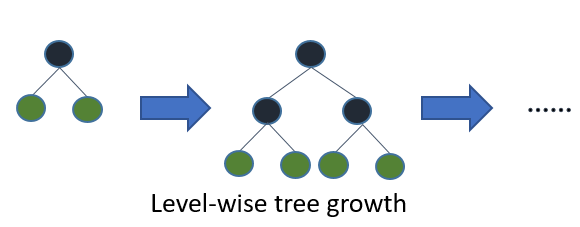
\includegraphics[scale=1.0]{figures/level_wise.png}
	\caption{ Стратегия выращивания деревьев в глубину (level-wise) }\label{fig:level_wise}
\end{figure}

LightGBM строит деревья \emph{по листьям} (leaf-wise или best-first) \pic{fig:lgb_leaf_wise} с ограничением на число терминальных узлов. Это приводит к тому, что деревья получаются \emph{несиммертичными}: одно поддерево может иметь глубину 2, а другое -- глубину 15. Выращивание деревьев по листьям может стать причиной переобучения, когда обучающих экземпляров $ \#data $ мало, поэтому LightGBM ограничивает еще и глубину дерева (\verb|max_depth|).

\begin{figure}[h]
	\centering
	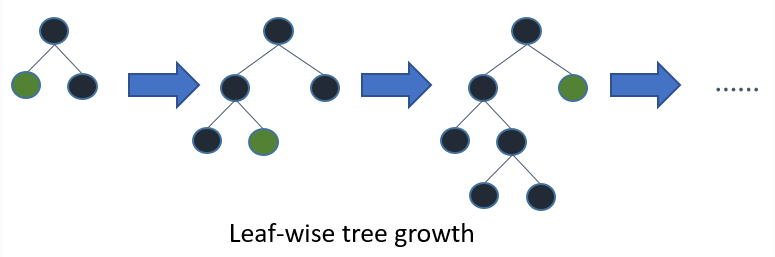
\includegraphics[scale=1.0]{figures/lgb_leaf_wise.png}
	\caption{ Стратегия LightGBM выращивания деревьев в глубину (level-wise). Получаются несиммертичные деревья }\label{fig:lgb_leaf_wise}
\end{figure}

\subsection{Оптимальное разбиение для категориальных признаков}

Обычно категориальные признаки представляют с помощью техники одного активного состояния (OHE), но этот подход неоптимален для <<деревянных>> моделей. Особенно для высоко кардинальных категориальных признаков дерево, построенное на признаках, закодированных с помощью OHE, должно быть \emph{очень глубоким}.

LightGBM сортирует гистограмму (для категориального признака) согласно накопленному значению \verb|sum_gradient / sum_hessian| и затем ищет лучшее разбиение по этой отсортированной гистограмме. Если я правильно понял, то они просто собирают категории в $ k $ групп и для каждой группы вычисляют отношение суммы градиентов к сумме гессианов, а затем сортируют группы по этой оценке и рассматривают $ k - 1 $ вариантов разбиения. 

\subsection{Расспараллеливание}

\emph{Традиционный алгоритм} поиска лучшего разбиения в дереве:
\begin{itemize}
	\item Матрица признакового описания объекта разбивается вертикально, то есть каждая машина получает свой поднабор признаков,
	
	\item Воркер ищет лучшую локальную точку разбиения (то есть пару <<признак--порог>>) на своем локальном подмножестве признаков,
	
	\item Из этих локальных лучших пар <<признак--порог>> выбирается лучшая пара,
	
	\item Воркер с лучшим разбиением делает разбиение, а затем отправляет другим воркерам результат разбиения данных,
	
	\item Другие воркеры разбивают данные в соответсвие с полученными данными.
\end{itemize}

Распараллеливание по признакам не может значительно повысить производительность, когда данных много, поэтому LightGBM предлагает вместо разбиения набора данных вертикально передавать \emph{полный набор} данных каждому воркеру. В этом случае снимаются накладные расходы на коммуникацию, так как каждый воркер знает как разбить данные.

Однако, остаются вычислительные издержки, когда данных много. Предлагается распараллеливать по данным.

\emph{Традиционный алгоритм} распараллеливания по данным:
\begin{itemize}
	\item Данные разбиваются горизонтально,
	
	\item Воркеры используют локальные поднаборы для построения локальных гистограмм,
	
	\item Локальные гистограммы сливаются в глобальную,
	
	\item Ищется лучшее разбиение на <<склееной>> глобальной гистограмме.
\end{itemize}

Недостаток: высокие издержки на коммуникацию.
\vspace{3mm}

LightGBM распараллеливает по данным так. Вместо объединения локальных гистограмм в одну глобальную гистограмму, LightGBM использует <<Reduce Scatter>> для объединения гистограмм различных неперекрывающихся признаков различных воркеров. Временная сложность $ O(0.5 \cdot \#features \cdot \#bins) $.

\subsection{Параметры}

\verb|force_col_wise|: используется только на CPU; \verb|force_col_wise=True| для принудительного поколоночного построения гистограммы; рекомендуется использовать, когда 
\begin{itemize}
	\item много признаков или бинов,
	
	\item используется много потоков \verb|num_threads| > 20,
	
	\item требуется снизить потребление памяти.
\end{itemize}

ВАЖНО: когда и \verb|force_col_wise=False| и \verb|force_row_wise=False|, LightGBM пробует оба эти параметра, а затем выбирает более быстрый. Чтобы не тратить время на тестирование вариантов, можно в ручную выбрать более быстры и его выставить в \verb|True|. Использовать можно только один из этих параметров.

\verb|force_row_wise|: используется только на CPU, \verb|force_row_wise=True| для принудительного построкового построения гистограммы; рекомендуется использовать, когда
\begin{itemize}
	\item много точек данных и общее количество бинов невелико,
	
	\item \verb|num_threads| относительно невелико ($ \leqslant 16 $),
	
	\item требуется использовать низкие значения \verb|bagging_fraction| или \verb|goss| стратегию выборки для ускорения.
\end{itemize}

ВАЖНО: если выставить \verb|force_row_wise| в \verb|True|, потребление памяти \verb|Dataset| удвоится. Если памяти недостаточно, то можно попробовать выставить \verb|force_col_wise| в \verb|True|.

\verb|min_data_in_leaf| (default = 20): минимальное число экземпляров в листе; может использоваться для борьбы с переобучением.

\verb|min_sum_hessian_in_leaf|: минимальная сумма гессианов в листе; так же как и \verb|min_data_in_leaf| может применяться для борьбы с переобучением.

\verb|bagging_fraction|: доля случайно выбранных экземпляров обучающего набора; может применяться для сокращения временных издержек на фазе обучения модели, а также для борьбы с переобучением; требуется установить ненулевое значение для параметра \verb|bagging_freq|.

\verb|pos_bagging_fraction|: используется только в задачах бинарной классификации; может быть полезен для несбалансированных задач; выбирает \verb|#pos_samples * pos_bagging_fraction| положительных экземпляров; должен использоваться вместе с \verb|neg_bagging_fraction|; чтобы использовать \verb|pos_bagging_fraction| нужно выставить еще \verb|bagging_freq| и \verb|neg_bagging_freq|.

\verb|bagging_freq|: частота беггинга; \verb|k| означает, что беггинг выполняется на каждой $ k $-ой итерации. То есть LightGBM на каждой $ k $-ой итерации случайно выбирает \verb|bagging_fraction * 100 %| от обучающего набора данных для следующих $ k $ итераций.

\verb|feature_fraction|: LightGBM на каждой итерации (то есть каждого дерева) будет случайно отбирать указанную долю признаков, если \verb|feature_fraction| < 1.0; может использоваться для снижения временных издержек на фазе обучения модели, а также для борьбы с переобучением.

\verb|feature_fraction_bynode|: LightGBM будет случайно выбирать указанную долю признаков в каждом узле дерева, если \verb|feature_fraction_bynode| < 1.0.

\verb|lambda_l1|: $ L_1 $-регуляризация.

\verb|lambda_l2|: $ L_2 $-регуляризация.

\verb|two_round|: рекомендуется выставить этот параметр в \verb|True|, если набор данных слишком большой для обучения в памяти; по умолчанию LightGBM отображает данные на память и загружает признаки из памяти; это значительно ускоряет загрузку, но может привести ошибкам памяти, если набор слишком большой; работает только, если данные загружаются напрямую из текстового файла.

\verb|predict_contrib|: если выставить в \verb|True|, то вернутся значения по Шепли, представляющие влкад каждого признака в прогноз.

\verb|is_unbalanced|: используется только в задачах \emph{бинарной} и \emph{многоклассовой классификации по схеме One-vs-All} (или что то же самое One-vs-Rest); если обучающий набор данных \emph{несбалансирован}, то нужно выставить в \verb|True|; этот параметр нельзя использовать одновременно с параметром \verb|scale_pos_weight|; нужно выбрать что-то одно.

\url{https://en.wikipedia.org/wiki/Multiclass_classification#One-vs.-rest} One-vs-Rest (или One-vs-All) -- это стратегия, идея которой состоит в том, чтобы один класс (положительный) был противопостовлен остальным классам, которые <<сливаются>> в единый отрицательный класс. Каждый класс из нескольких должен побывать на месте положительного класса, противопоставленного отрицательному классу, состоящему из остальных классов. Эта стратегия требует, чтобы базовые классификаторы выдавали реальный показатель достоверности своего решения, а не просто метку класса. При построении прогноза к новому тестовому экземпляру $ x $ применяются все обученные классификаторы и прогнозируется метка класса с наивысшей оценкой (confidence score)
\begin{align*}
	\hat{y} = \argmax_{k \in \{1, \ldots, K\}} \, f_k(x)
\end{align*}

ВАЖНО! Не смотря на то, что эта страетгия очень популярна, она обладает серьезными недостатками:
\begin{itemize}
	\item Масштаб оценок принятия решений (confidence values) может быть различным для бинарных классификаторов,
	
	\item Даже если исходный набор данных сбалансирован, то схема One-vs-All (One-vs-Rest) делает набор несбалансированным, потому как экземпляров положительного класса обычно значительно меньше экземпляров отрицательного класса.
\end{itemize}

One-vs-one обучает $ (K - 1) \, K / 2 $ классификаторов для задачи мультиклассовой классификации на $ K $-классов. Например, если решается задача на 3 класса, то нужно построить 3 классификатора: <<1--2>>, <<1--3>>, <<2--3>>. На шаге построения прогноза применяется схема голосования: все $ (K - 1) \, K / 2 $ классификаторы применяются к тестовой точке $ x $ и прогнозируется класс, получивший наибольшее число голосов.

ВАЖНО! Так же как и One-vs-Rest, One-vs-One страдает от неопределенности, так как в некоторых случаях прогнозы могут быть несогласованы. Например, <<1--2>> $ \rightarrow $ 2, <<1--3>> $ \rightarrow $ 1 и <<2--3>> $ \rightarrow $ 3.

\verb|scale_pos_weight|: взвешивает метки экземпляров положительного класса; используется только в задачах \emph{бинарной} \verb|binary| и \emph{многоклассовой классификации по схеме One-vs-All} (One-vs-Rest) \verb|multiclassova|;  этот параметр нельзя использовать одновременно с параметром \verb|is_unbalanced|; нужно выбрать что-то одно.

\verb|reg_sqrt|: используется только в задачах регрессии; на шаге обучения модели вместо исходных меток использует $ \sqrt{label} $, а на шаге построения прогноза -- $ prediction^2 $; может быть полезен в случаях, когда значения целевой переменной изменяются в широком диапазоне.

\subsection{Замечания о подборе гиперпараметров в LightGBM}

LightGBM строит деревья по листьям (leaf-wise), однако, для того чтобы модель не переобучалась нужно настраивать следующие параметры:
\begin{itemize}
	\item \verb|num_leaves|: это главный параметр в LightGBM, контролирующий сложность деревьев. Теоретически, мы могли бы задать $ \verb|num_leaves = 2^(max_depth)| $, чтобы получить то же дерево, что и в XGBoost (строит \underline{\itshape полные бинарные деревья} \emph{в глубину}, по уровням, и потому число уровней в таком дереве будет логарифмически зависеть от числа листьев дерева,
	
	$ \text{max\_depth} = log_2(\text{num\_leaves}) \, \rightarrow \text{num\_leaves} = 2^{\text{max\_depth}}$.
	
	Однако, это правило для LightGBM на практике работает плохо, так как leaf-wise деревья (то есть деревья, которые строятся по листьям) гораздо глубже depth-wise деревьев (деревьев, которые строятся по уровням) при фиксированном числе листьев. Такими деревьями легко переобучиться. {\color{blue}Таким образом, при подборе значения параметра \verb|num_leaves| нужно задавать значения $ < 2^{\text{max\_depth}} $}. Например, если \verb|max_depth=7| в depth-wise дереве (XGBoost), то в leaf-wise дереве (LIghtGBM) число листьев должно быть меньше 127, скажем 70-80.
	
	\item \verb|min_data_in_leaf|: это очень важный параметр для предотвращения переобучения leaf-wise деревьев. Оптимальное значение зависит от \emph{числа экземпляров обучающего набора данных} и \emph{числа листьев} \verb|num_leaves|. Большие значения делают деревья менее глубокими, что может привести к недообучению. На практике этот параметр имеет порядок нескольких сотен ($ \approx 100 $).
	
	\item \verb|max_depth|: можно использовать \verb|max_depth|, чтобы явно ограничить глубину дерева.
\end{itemize}

Для того чтобы поднять скорость вычислений можно выставить параметр \verb|num_threads| в число \emph{доступных} ядер процессора. То есть обчение можно ускорить, перейдя на машину с большим количеством доступных ядер процессора. Еще можно воспользоваться моделью распределенного обучения. Или можно попробовать LigthGBM с поддержкой GPU.

\subsubsection{\texttt{max\_depth} и \texttt{num\_leaves} для снижения времени обучения}

Чем меньше \verb|max_depth|, тем меньше время обучения модели. Тоже самое касается и параметра \verb|num_leaves|: чем меньше листьев разрешается в дереве, тем меньше время обучения модели.

\subsubsection{\texttt{min\_gain\_to\_split}}

Когда добавляется новый узел в дерево, LightGBM выбирает точку разбиения с наибольшим информационным приростом. Информационный прирост по сути показывает снижение потерь на обучающем наборе данных при добавлении рассматриваемой точки разбиения. По умолчанию LightGBM выставляет параметр \verb|min_gain_to_split| в 0, что означает <<мы рады любому, даже самому маленькому информационному приросту>>. Однако, на практике можно заметить, что небольшое снижение потерь на обучающем наборе данных не оказывает значимого влияния на обобщающую способность модели. Большие значения \verb|min_gain_to_split| снижают время обучения модели (потому как в модели будет меньше листьев).

\subsubsection{\texttt{min\_data\_in\_leaf} и \texttt{min\_sum\_hessian\_in\_leaf}}

\begin{itemize}
	\item \verb|min_data_in_leaf|: минимальное число наблюдений (экземпляров), которое должно попасть в узел, чтобы он был добавлен в дерево,
	
	\item \verb|min_sum_hessian_in_leaf| (то же что и \verb|min_child_weight| XGBoost'а): минимальная сумма гессианов (вторая производная от функции потерь, которая вычисляется для каждого наблюдения) наблюдений в листе.
\end{itemize}

\href{https://stats.stackexchange.com/questions/317073/explanation-of-min-child-weight-in-xgboost-algorithm}{Пояснение}
\begin{itemize}
	\item Для регрессии потеря на $ i $-ом экземпляре в узле будет $ 1/2 (y_i - \hat{y}_i)^2 $. Вторая производная от этого выражения (гессиан) по $ \hat{y}_i $ будет 1. Таким образом, сумма вторых производных (гессианов) по всем экземплярам узла это просто \emph{число экземпляров в этом узле}. То есть в данном случае \verb|min_child_weight| (это XGBoost'ый параметр; получается, что это тоже самое что и \verb|min_sum_hessian_in_leaf| в LightGBM) означает <<прекратите разбивать узел, как только число экземпляров в узле окажется меньше заданного порога>>. Потому что нам не нужны листья с малым числом экземпляров (вырожденный случай лист с одним экземпляром).
	
	\item Для бинарной классификации (модель логистической регрессии) гессиан для каждой точки в узле будет $ \sigma(\hat{y}_i) (1 - \sigma (\hat{y}_i)) $, где $ \sigma $ -- это логистический сигмоид. Пусть узел будет чистым положительным (то есть в узле лежат экземпляры только одного положительного класса). Тогда все $ \hat{y}_i $ будут большими положительными числами, и потому $ \sigma(\hat{y}_i) $ будут числами близкими к 1. Таким образом, все гессианы будут близки к 0. Рассуждения справедливы и для случая, когда все экземпляры в узле отрицательные. В этом случае \verb|min_child_weight| можно интерпретировать как: <<прекратите разбивать узел, как только узел достигнет определенной степени чистоты>>. Или лучше сказать, что не нужно разбивать узел, если его чистота выше некоторого порога, то есть не нужно разбивать узел, если он <<слишком чистый>>. Нам не нужны чистые листья! Можем переобучиться.
\end{itemize}

\subsubsection{\texttt{learning\_rate} и \texttt{num\_iterations}}

Выбор правильного значения для пары \verb|learning_rate| и \verb|num_iterations| сильно зависит от данных и целевой функции, поэтому эти гиперпараметры обычно подбирают. Общее правило: меньшие значения \verb|learning_rate| отвечают большему числу итераций градиентного бустинга. Меньшие значения числа итераций градиентного бустинга отвечают меньшему времени обучения.

\subsubsection{\texttt{max\_bin} или \texttt{max\_bin\_by\_feature}}

LightGBM чтобы ускорить обучение модели и снизить потребление памяти непрерывные признаки разбивает по бинам. Разбиение по бинам выполняется на этапе конструирования \verb|Dataset|. Число разбиений, учитываемых при разбиении узла равно $ O(\#feature \cdot \#bin) $. Таким образом, уменьшение числа бинов для каждого признака может снизить число разбиений, которые нужно рассматреть.

Меньшие значения \verb|max_bin| или \verb|max_bin_by_feature| снижают время обучения модели.

\subsubsection{\texttt{feature\_fraction}}

Меньшие значения \verb|feature_fraction| снижают время обучения модели, так как уменьшается общее число разбиений, которое нужно оценить для того чтобы добавить узел в дерево.

\subsubsection{\texttt{bagging\_fraction} и \texttt{bagging\_freq}}

По умолчанию LightGBM на каждой итерации градиентного бустинга использует все экземпляры обучающего набора данных, однако можно попросить использовать не все экземпляры, а какую-то долю случайно выбранных (эта процедура называется беггингом).

Например, если сказать: \verb|bagging_freq=5|, а \verb|bagging_fraction=0.75|, то это будет значить <<делай выборку без возвращения каждые 5 итераций и выбирай 75\% экземпляров обучающего набора>>.

Меньшие значения \verb|bagging_fraction| снижают время обучения модели.

\subsubsection{Для улучшения метрик}

Для получения более высоких значений метрик качества:
\begin{itemize}
	\item используйте большие значения \verb|max_bin| (может быть медленным),
	
	\item используйте меньшие значения \verb|learning_rate| с большими значениями \verb|num_iterations|,
	
	\item используйте большие значения \verb|num_leaves| (опасно! можно переобучиться),
	
	\item используйте больше обучающих экземпляров,
	
	\item попробуйте \verb|dart|.
\end{itemize}

\subsubsection{Для снижения эффекта переобучения}

Чтобы снизить переобучение:
\begin{itemize}
	\item используйте низкие значения \verb|max_bin|,
	
	\item используйте низкие значения \verb|num_leaves|,
	
	\item используйте \verb|min_data_in_leaf| и \verb|min_sum_hessian_in_leaf|,
	
	\item используйте подвыборку по экземплярам: \verb|bagging_fraction| и \verb|bagging_freq|,
	
	\item используйте подвыборку по признакам: \verb|feature_fraction|,
	
	\item используйте б\emph{о}льший набор данных; при фиксированной емкости модели чем больше набор данных, тем сложнее его описывать (обогащение набора новыми данными -- регуляризация на уровне данных),
	
	\item используйте \verb|lambda_l1|, \verb|lambda_l2| и \verb|min_gain_to_split| (если я правильно понял, то это то же, что и параметр \verb|gamma| в XGBoost) для регуляризации,
	
	\item ограничьте \verb|max_depth|, чтобы не строить глубоки деревья.
\end{itemize}

В документации LightGBM ничего нет о регуляризующем эффекте низких \verb|learning_rate|, но в документации XGBoost низкие значения темпа обучения встречаются в контексте борьбы с переобучением.


\subsection{Подбор гиперпараметров LightGBM с подрезкой <<слабых>> запусков}

\begin{lstlisting}[
style = ironpython,
numbers = none
]
import numpy as np
import optuna

import lightgbm as lgb
import sklearn.datasets
import sklearn.metrics
from sklearn.model_selection import train_test_split


# FYI: Objective functions can take additional arguments
# (https://optuna.readthedocs.io/en/stable/faq.html#objective-func-additional-args).
def objective(trial):
	data, target = sklearn.datasets.load_breast_cancer(return_X_y=True)
	train_x, valid_x, train_y, valid_y = train_test_split(data, target, test_size=0.25)
	dtrain = lgb.Dataset(train_x, label=train_y)
	dvalid = lgb.Dataset(valid_x, label=valid_y)

	param = {
		"objective": "binary",
		"metric": "auc",
		"verbosity": -1,
		"boosting_type": "gbdt",
		"lambda_l1": trial.suggest_float("lambda_l1", 1e-8, 10.0, log=True),
		"lambda_l2": trial.suggest_float("lambda_l2", 1e-8, 10.0, log=True),
		"num_leaves": trial.suggest_int("num_leaves", 2, 256),
		"feature_fraction": trial.suggest_float("feature_fraction", 0.4, 1.0),
		"bagging_fraction": trial.suggest_float("bagging_fraction", 0.4, 1.0),
		"bagging_freq": trial.suggest_int("bagging_freq", 1, 7),
		"min_child_samples": trial.suggest_int("min_child_samples", 5, 100),
	}

	# Add a callback for pruning.
	pruning_callback = optuna.integration.LightGBMPruningCallback(trial, "auc")
	gbm = lgb.train(param, dtrain, valid_sets=[dvalid], callbacks=[pruning_callback])

	preds = gbm.predict(valid_x)
	pred_labels = np.rint(preds)
	accuracy = sklearn.metrics.accuracy_score(valid_y, pred_labels)
	return accuracy


if __name__ == "__main__":
	study = optuna.create_study(
		pruner=optuna.pruners.MedianPruner(n_warmup_steps=10), direction="maximize"  # <- NB
	)
	study.optimize(objective, n_trials=100)
	
	print("Number of finished trials: {}".format(len(study.trials)))
	
	print("Best trial:")
	trial = study.best_trial
	
	print("  Value: {}".format(trial.value))
	
	print("  Params: ")
	for key, value in trial.params.items():
		print("    {}: {}".format(key, value))
\end{lstlisting}


\subsection{Подбор гиперпараметров для LightGBM с помощью Optuna LightGBMTuner}

\url{https://medium.com/optuna/lightgbm-tuner-new-optuna-integration-for-hyperparameter-optimization-8b7095e99258}

Наивный способ подбора гиперпараметров с помощью Optuna мог бы выглядет так
\begin{lstlisting}[
style = ironpython,
numbers = none
]
def objective(trial):
	data, target = sklearn.datasets.load_breast_cancer(return_X_y=True)
	train_x, test_x, train_y, test_y = train_test_split(data, target, test_size=0.25)
	dtrain = lgb.Dataset(train_x, label=train_y)

	param = {
		'objective': 'binary',
		'metric': 'binary_logloss',
		'lambda_l1': trial.suggest_loguniform('lambda_l1', 1e-8, 10.0),
		'lambda_l2': trial.suggest_loguniform('lambda_l2', 1e-8, 10.0),
		'num_leaves': trial.suggest_int('num_leaves', 2, 256),
		'feature_fraction': trial.suggest_uniform('feature_fraction', 0.4, 1.0),
		'bagging_fraction': trial.suggest_uniform('bagging_fraction', 0.4, 1.0),
		'bagging_freq': trial.suggest_int('bagging_freq', 1, 7),
		'min_child_samples': trial.suggest_int('min_child_samples', 5, 100),
	}

	gbm = lgb.train(param, dtrain)
	preds = gbm.predict(test_x)
	pred_labels = np.rint(preds)
	accuracy = sklearn.metrics.accuracy_score(test_y, pred_labels)
	return accuracy

study = optuna.create_study(direction='maximize')
study.optimize(objective, n_trials=100)

print('Number of finished trials:', len(study.trials))
print('Best trial:', study.best_trial.params)
\end{lstlisting}

В этом примере Optuna пытается найти наилучшую комбинацию 7 различных гиперпараметров (параметр регуляризации $ L_1 $, число терминальных узлов \verb|num_leaves| и пр.). Суммарное количество комбинаций это произведение всех пространств поиска каждого гиперпараметра.

Не смотря на то, что существует много методов поиска наилучшей комбинации гиперпараметров за наименьшее количество запусков, все же имеет смысл рассмотреть альтернативный \emph{метод последовательного подбора} (stepwise algorithm) -- он, как понятно из названия, подбирает параметры последовательно и итоговое пространство поиска будет представлять собой \emph{сумму} (а не произведение!!!) пространств поиска. 

{\color{blue}Класс \verb|optuna.integration.lightgbm.LightGBMTuner| реализует именно \emph{последовательный алгоритм подбора гиперпараметров}.}

\verb|LIghtGBMTuner| \emph{последовательно} (stepwise manner) подбирает следующие гиперпараметры :
\begin{itemize}
	\item \verb|lambda_l1|,
	
	\item \verb|lambda_l2|,
	
	\item \verb|num_leaves|,
	
	\item \verb|featuer_fraction|,
	
	\item \verb|bagging_fraction|,
	
	\item \verb|bagging_freq|,
	
	\item \verb|min_child_samples| (то же что и \verb|min_data_in_leaf|).
\end{itemize}

Для того чтобы использовать \verb|LightGBMTuner| нужно изменить лишь строку импотра библиотеки \verb|ligthgbm|

\begin{lstlisting}[
style = ironpython,
numbers = none
]
import lightgbm as lgb  # было
import optuna.integration.lightgm as lgb  # стало!

from lightgbm import early_stopping
from lightgbm import log_evaluation
import sklearn.datasets
from sklearn.metrics import accuracy_score
from sklearn.model_selection import train_test_split


if __name__ == "__main__":
	data, target = sklearn.datasets.load_breast_cancer(return_X_y=True)
	train_x, val_x, train_y, val_y = train_test_split(data, target, test_size=0.25)
	dtrain = lgb.Dataset(train_x, label=train_y)
	dval = lgb.Dataset(val_x, label=val_y)

	params = {
		"objective": "binary",
		"metric": "binary_logloss",
		"verbosity": -1,
		"boosting_type": "gbdt",
	}

	model = lgb.train(   # здесь начинается ПОСЛЕДОВАТЕЛЬНЫЙ подбор гиперпараметров
		params,
		dtrain,
		valid_sets=[dtrain, dval],
		callbacks=[early_stopping(100), log_evaluation(100)],
		time_budget=600,
		model_dir="./boosters",  # сюда будут записываться модели бустера, например, 14.pkl
	)
	
	prediction = np.rint(model.predict(val_x, num_iteration=model.best_iteration))
	accuracy = accuracy_score(val_y, prediction)
	
	best_params = model.params
	print("Best params:", best_params)
	print("  Accuracy = {}".format(accuracy))
	print("  Params: ")
	for key, value in best_params.items():
		print("    {}: {}".format(key, value))
\end{lstlisting}

Подбор гиперпараметров начинается, когда вызывается функция \verb|lgb.train()|, а построить прогноз можно так
\begin{lstlisting}[
style = ironpython,
numbers = none
]
cohen_kappa_score(y_test, np.rint(model.predict(X_test)))  # 0.9750292056074766
\end{lstlisting}

\subsection{Распределенное обучение с LightGBM}

Получить доступ к LightGBM для работы в распределенном режиме на кластере Spark можно с помощью библиотеки SynapseML \url{https://microsoft.github.io/SynapseML/}.

\subsection{Конспект статьи G. Ke LightGBM. A Highly Efficient Gradient ...}

В статье предлагается две техники:
\begin{itemize}
	\item Gradient-based One-Side Sampling (GOSS): авторы считают, что экземпляры данных с большими градиентами играют более важную роль в вычислении информационного прироста и GOSS может получить более аккуратные оценки информационного прироста на значительно меньшем наборе данных,
	
	\item Exclusive Feature Bundling (EFB): с помощью этой техники авторы предлагают объединять \emph{взаимоисключающие признаки} (то есть признаки, которые редко принимают ненулевые значения одновременно) для снижения размероности задачи по признакам. Поиск оптимального объединения взаимоисключающих признаков это NP-трудная задача, но авторы показывают, что жадный алгоритм может найти приемлемую аппроксимацию решения (и таким образом эффективно снизить размерность задачи по признакам без значительного снижения точности определения точки разбиения в узле).
\end{itemize}

Эту реализацию деревьев решения градиентного бустинга (Gradient Boostring Decision Tree, GBDT) с GOSS и EFB авторы называют LightGBM. 

\emph{Gradient-based One-Side Sampling} (GOSS). Экземпляры данных с различными градиентами дают различный вклад при вычислении информационного прироста. В частности, согласно определению информационного прироста, \emph{экземпляры с большим градиентом}\footnote{В этой статье под большими или малыми градиентами авторы понимают абсолютные значения градиентов} (то есть \underline{недообученные} экземпляры) будут давать \emph{больший вклад} в информационный прирост (information gain). Поэтому для того чтобы сохранить точность информационного прироста выгоднее сохранять экземпляры с большим градиентом (то есть с градиентом, превышающем некоторый порог, или с градиентом верхних персентилей), а случайно отбрасывать экземпляры с малым градиентом. Авторы показывают, что такая подвыборка экземпляров может давать более аккуратные оценки информационного прироста, чем простая равномерная выборка.

\emph{Exclusive Feature Bundling} (EFB). Обычно, несмотря на большое количество признаков в матрице признакового описания объекта, пространство признаков \emph{довольно разреженное}. В разреженном признаковом пространстве многие признаки (почти) уникальные, то есть они редко принимают ненулевые значения одновременно. Авторы сводят \emph{задачу оптимального объединения взаимоисключающих признаков} к \emph{задаче о раскраске графа} (используя в качестве вершин графа признаки и соединяя каждые два признака ребром, если они \emph{не взаимоисключающие}) и решают ее с помощью жадного алгоритма.

\subsubsection{GBDT и анализ сложности}

GBDT -- это ансамбль моделей решающих деревьев, которые обучаются \emph{последовательно}. На каждой итерации градиентного бустинга решающие деревья (то есть базовые алгоритмы) подгоняются под вектор \emph{антиградиента} (еще его называют псевдо-остатками, residual errors).

Основные затраты в градиентном бустинге связаны с обучением (лучше сказать с \emph{построением}) решающих деревьев, а самая затратная по времени часть это \emph{поиск налучших точек разбиения} (the best split points).

Один из самых популярных алгоритмов поиска точек разбиения -- это \emph{алгоритм предварительной сортировки} (pre-sorted algorithm), который перебирает все возможные точки разбиения на предварительно отсортированных значениях признака. Этот алгоритм простой и может найти оптимальные точки разбиения, но он неэффективен ни с точки зрения скорости обучения, ни с точки зрения потребления памяти.

Другой популярный алгоритм поиска точек разбиения -- это \emph{гистограмный алгоритм} (histogram-based algorithm). Вместо того чтобы искать точки разбиения на отсортированном признаке, гистограмный алгоритм разбивает непрерывные вещественные признаки на бины и использует эти бины для построения гистограмм признаков во время обучения. Этот алгоритм эффективен и по скорости обучения, и по потреблению памяти (и потому авторы LightGBM решили свою работу развивать именно на нем).

У операции \emph{построения гистограммы} временная сложность $ O(\#data \times \#feature) $, а у операции \emph{поиска разбиения} -- $ O(\#bin \times \#feature) $. Поскольку бинов $ \#bin $ обычно значительно меньше, чем экземпляров $ \#data $, временная сложность операции построения гистограммы значительно больше временной сложности операции поиска разбиения. Если мы сможем снизить $ \#data $ или $ \#feature $, то получится значительно ускорить обучение градиентного бустинга.

В Python-библиотеке Scikit-learn и R-библиотеке gbm реализован \emph{алгоритм предварительной сортировки} (плохо, неэффективный алгоритм), а XGBoost поддерживает и алгоритм предварительной сортировки (\verb|tree_method=exact|), и гистограммный алгоритм (\verb|tree_mthod=hist|). 

Для снижения размера обучающего набора данных обычно делают подвыборку. Например, экземпляры могут быть отфильтрованы по их весу, который не превышает некоторый заданный порог. Стохастический градиентный бустинг Фридмана (Stochastic Gradient Boosting) на каждой итерации для обучения слабых учеников (weak learners) использует случайную подвыборку.

Для того чтобы сократить число признаков, кажется ествественным отфильтровать слабые признаки. Обычно эта процедура выполняется, например, с помощью метода главных компонент (PCA). Однако, PCA предполагает, что признаки содержать избыточную информацию, что не всегда так (признаки обычно проектируются с учетом их индивидуального вклада и удаление любого из них может повлиять на точность обучения).

Обычно крупномасштабные наборе данных, которые используются в реальных приложениях довольно \emph{разрежены}. GBDT с алгоритмом предварительной сортировки может снизить временные издержки на обучение, игнорируя признаки с нулевыми значениями. Однако, GBDT с гистограммным алгоритмом не имеет эффективного решения для разреженной оптимизации. Причина в том, что гистограммный алгоритм должен извлекать значения признаков из бинов.

\subsubsection{Gradient-based One-Side Sampling, GOSS}

\paragraph{Описание алгоритма} В адапитвном бустинге вес экземпляра служит хорошим показателем важности этого экземпляра. Однако в градиентном бустинге у экземпляров нет своих весов и потому метод отбора, предлагаемый AdaBoost, не может быть применен на прямую. К счатью, мы замечаем, что градиент каждого экземпляра в градиентном бустинге сообщает полезную информацию по выборке. Если у \emph{экземпляра небольшой градиент}, то значит и \emph{ошибка} на этом экземпляре тоже \emph{небольшая}. Идея состоит в том, чтобы отбросить экземпляры с малым градиентом. Однако, это приведет к тому, что распределение данных изменится и снизит точность обучаемой модели. Чтобы обойти эту проблему авторы предлагают метод GOSS.

{\color{blue}GOSS учитывает \emph{все} экземпляры с \emph{большим градиентом} и \emph{случайно} отбирает экземпляры с \emph{малым градиентом}.} Для того чтобы компенсировать искажение распределения данных, при вычислении информационного прироста GOSS вводит постоянный множитель для экземпляров с малым градиентом. Сначала GOSS сортирует экземпляры обучающего набора по абсолютной величине градиента и выбирает верхние $ a \times 100 \% $ экземпляров. Затем он случайно отбирает $ b \times 100\% $ экземпляров из оставшегося набора данных. После чего при вычислении информационного прироста GOSS умножает экземпляры с малым градиентом на $ \dfrac{1 - a}{b} $. Поступая таким образом, мы делаем акцент на недообученных экземплярах, не изменяя существенно исходное расрпеделение данных.

\paragraph{Теоретический анализ} GBDT использует решающие деревья для обучения функции, отображающей входное пространство $ \mathcal{X}^s $ в пространство градиентов $ \mathcal{G} $. Предположим, что у нас есть обучающее множество $ n $ независимых одинаково распределенных (i.i.d) экземпялров $ \{x_i, \ldots, x_n\} $, в котором каждый $ x_i $ это вектор размерности $ s $ в пространстве $ \mathcal{X}^s $. На каждой итерации градиентного бустинга отрицательный градиент целевой функции по отношению к выходу модели обозначается как $ \{g_1, \ldots, g_n\} $. Модель решающего дерева каждый узел разбивает \emph{по самому информативному признаку} (то есть \emph{по признаку с наибольшим информационным приростом}).

Для GBDT информационный прирост обычно оценивается по \emph{дисперсии} после разбиения
\begin{align*}
	V_{ j | O }(d) = \dfrac{1}{n_O} \Bigg( \dfrac{ (\sum_{ \{x_i \in O: x_{ij} \leqslant d \} } g_i)^2 }{ n_{l | O}^j(d) } + \dfrac{ (\sum_{\{x_i \in O: x_{ij} > d \} } g_i )^2 }{ n_{r | O}^j(d) } \Bigg),
\end{align*}
где $ O $ -- обучающий набор данных, попавших в рассматриваемый узел дерева; $ j $ -- признак, по которому строится разбиение; $ d $ -- пороговое значение; $ n_O = \sum I[x_i \in O] $ -- число экземпляров, попавших в рассматриваемый узел дерева; $ n_{ l | O }^j(d) = \sum I[x_i \in O: x_{ij} \leqslant d] $ -- число экземпляров, попавших в левый дочерний узел; $ n_{r | O}^j (d) = \sum I[x_i \in O: x_{ij} > d] $ -- число экземпляров, попавших в правый дочерний узел.

Для признака $ j $ алгоритм решающего дерева выбирает такое пороговое значение $ d $, которое максимизирует дисперсию -- то есть $ d_j^* = \argmax_d V_j(d) $ -- и вычисляет наибольший информационный прирост $ V_j(d_j^*) $. Затем данные разбиваются по признаку $ j^* $ и значению $ d_{j^*} $ на левый и правый дочерние узлы.

В предлагамемом методе GOSS:
\begin{itemize}
	\item обучающие экземпляры сначала сортируются по их абсолютному значению градиента в порядке убывани,
	
	\item затем сохраняется заданная доля верхних $ a \times 100\% $ экземпляров с большим градиентом и получается множество экзмепляров $ A $,
	
	\item потом из оставшегося множества $ A^c $, состояющего из $ (1 - a) \times 100\% $ экземпляров с малым градиентом, случайно отбираются экземпляры множества $ B $ размера $ b \times |A^c| $,
	
	\item и наконец, экземпляры разбиваются по оценке дисперсии прироста (variance gain) $ \tilde{V}_j(d) $
\begin{align*}
	\tilde{V}_j(d) = \dfrac{1}{n} \Bigg( \dfrac{(\sum_{ x_i \in A_l } g_i +\dfrac{ 1 - a}{b} \sum_{ x_i \in B_l } g_i)^2 }{ n_l^j(d) } + \dfrac{ ( \sum_{x_i \in A_r} g_i + \dfrac{1 - a}{b} \sum_{x_i \in B_r} g_i )^2 }{ n_r^j(d) } \Bigg),
\end{align*}
где $ A_l = \{ x_i \in A: x_{ij} \leqslant d \} $ -- множество экземпляров с большим градиентом (попавших в левый дочерний узел) со значением $ j $-ого признака непревышающем значение порога $ d $;  $ A_r = \{ x_i \in A: x_{ij} > d \} $ -- множество экземпляров с большим градиентом (попавших в правый дочерний узел) со значением $ j $-ого признака меньшим значения порога $ d $; $ B_l = \{ x_i \in B: x_{ij} \leqslant d \} $ -- множество экземпляров с малым значением градиента (попавших в левый дочерний узел) со значением $ j $-ого признака непревышающего значения порога $ d $; $ B_r = \{ x_i \in B: x_{ij} > d \} $ -- множество экземпляров с малым градиентом (попавших в правый дочерний узел) со значением $ j $-ого признака меньшим значения порога $ d $ и коэффициент $ \dfrac{1 - a}{b} $ используемый для нормализации суммы градиентов по $ B $.
\end{itemize}

Таким образом, в GOSS для вычисления точки разбиения используется оценка дисперсии прироста по малому подмножеству экземпляров $ \tilde{V}_j(d) $  вместо точной оценки $ V_j(d) $ по всем экземплярам и потому вычислительные затраты могут быть значительно снижены. В статье приводится теорема, которая показывает, что GOSS <<не просадит>> точность модели на обучающем поднаборе данных и превзойдет случайную выборку.

Из теоремы следует, что:
\begin{itemize}
	\item на больших наборах данных предалагаемая аппроксимация обладает достаточной точностью,
	
	\item случайная подвыборка это специальный случай GOSS при $ a = 0 $.
\end{itemize}

\subsubsection{Exclusive Feature Bundling}

Высокоразмерные данные обычно \emph{сильно разрежены}. В разреженном пространстве признаков многие признаки являются взаимоисключающими, то есть они никогда не принимают ненулевые значения одновременно. Мы можем безопасно объединить взаимоисключающие признаки в один. Тогда временная сложность построения гистограммы изменится с $ O(\#data \times \#features) $ на $ O(\#data \times \#bundle) $, при том, что $ \#bundle \ll \#feature $.

Однако сначала нужно ответить на следующие вопросы: какие признаки должны быть объеденины? и как построить объединение (bundle)?

Задача объединения признаков в меньшее количество групп (bunldes) это NP-трудная задача. Доказательство: описанная задача сводится к задаче о раскраске графа, а она NP-трудная.

Признаки это вершины графа. Легко видеть, что набор вершин графа, окрашенных в один и тот же цвет, представляют собой связку взаимоисключающих признаков (exclusive budle of features). Задача поиска оптимального объединения признаков относится к классу NP-трудных, а значит невозможно получить точное решение за полиномиальное время.

Для того чтобы найти хорошее приближение, авторы сводят задачу оптимального объединения к задаче о раскраске графа, принимая признаки в качестве вершин графа и соединяя ребрами каждые два признака, если они \emph{не являются взаимоисключающими}. В итоге удается получить достаточно эффективный жадный алгоритм (с постоянным коэффициентом приближения). Кроме того, обычно многие признаки (хотя и не являются на 100\% взаимоисключающими) также редко принимают ненулевые значения одновременно. Если алгоритм сможет разрешить небольшую долю конфликтов, то мы сможем еще сократить количество объединений и как следствие снизить вычислительную нагрузку.

Итак, сначала мы строим граф с взвешенными ребрами, веса которого указывают на суммарное число конфликтов между признаками. Затем мы сортируем признаки по их степеням в графе (в порядке убывания). И наконец, мы проверяем каждый признак в упорядоченном списке и либо назначаем его существующему объединению с малым конфликтом (контролируется параметром $ \gamma $), либо создаем новое объединение. Временная сложность жадного объединения будет $ O(\#feature^2) $ и эта процедура выполняется только один раз, перед обучением. Такая временная сложность приемлема, если признаков немного.

Авторы предлагают более эффективную стратегию объединения без построения графа (Merge Exclusive Features): упорядочивание по числу ненулевых значений, что эквивалентно упорядочиванию по степеням, поскольку большее число ненулевых значений обычно приводит к более высокой вероятности конфликтов. Поскольку гистограммный алгоритм хранит дискретные бины вместо непрервных значений признаков, мы может сконструировать объединение признаков, разрешив эксклюзивным признакам находится в разных бинах. Этого можно добиться добавив смещение ко всем значениям исходных признаков. Например, пусть у нас есть объединение из двух признаков. Изначально, признак $ A $ принимает значения из $ [0, 10) $, а признак $ B $ -- из диапазона $ [0, 20) $. Тогда ко всем значениям признака $ B $ можно добавить смещение 10 и тогда признак $ B $ будет принимать значение из $ [10, 30) $. После этого можно \emph{слить} (merge) признаки $ A $ и $ B $ таким образом, чтобы получился \emph{новый признак} (замещающий два старых $ A $ и $ B $), принимающий значения из диапазона $ [0, 30] $.

EFB алгоритм объединяет множество экзклюзивных признаков в гораздо меньшее число ллотных признаков, что позволяет избежать ненужных вычислений для нулевых признаков. Еще можно оптимизировать гистограммный алгортим таким образом, чтобы он игнорировал нулевые значения признаков, используя таблицу для каждого признака для записи ненулевых значений. Тогда временная сложность построения гистограммы для одного признака изменится с $ O(\#data) $ на $ O(\#non\_zero\_data) $. Однако этот метод требует дополнительной памяти и вычислительных затрат для поддержания этих таблиц (одна таблица для каждого признака) на протяжении всего процесса роста дерева. 

\subsubsection{Обсуждение}

Как показывают вычислительные эксперименты алгоритм выборки GOSS значительно более эффективен, чем случайная выборка. EFB очень эффективен на разреженных признаковых пространствах (потому как сливает большое число разреженных признаков в небольшое число подгрупп плотных признаков).

LightGBM значительно эффективнее XGBoost и алгоритма стохастического градиентного бустинга как с точки зрения потребления памяти, так и с точки зрения временных издержек.








\section{Приемы работы с библиотекой подбора гиперпараметров Optuna}

\url{https://optuna.org/}

Базовые понятия:
\begin{itemize}
	\item Study -- оптимизация базируется на целевой функции,
	
	\item Trial -- одиночный запуск целевой функции.
\end{itemize}

Optuna прекрасно работает и с Scikit-learn, и с XGBoost, и с LightGBM, и с прочими популярными библиотеками.

Обычно Optuna используется для подбора гиперпараметров, но может быть использована и для оптимизации пользовательских функций. Для примера рассмотрим простую квадратическую функцию $ (x - 2)^2 $
\begin{lstlisting}[
style = ironpython,
numbers = none
]
import optune

def objective(trail):
    x = trail.suggest_float("x", -10, 10)
    return (x - 2) ** 2

study = optuna.create_study()
study.optimize(objective, n_trails=100)
\end{lstlisting}

Лучшие найденные параметры можно получить так
\begin{lstlisting}[
style = ironpython,
numbers = none	
]
study.best_params  # {'x': 1.9914500091892555}
\end{lstlisting}

Можно запустить оптимизацию еще на 100 запусков
\begin{lstlisting}[
style = ironpython,
numbers = none
]
study.optimize(objective, n_trails=100)
len(study.trials)  # 200
\end{lstlisting}

Для выбора значений гиперпараметров Optuna предлагает следующие функции:
\begin{itemize}
	\item \verb|optuna.trial.Trial.suggest_categorical()| для категориальных параметров,
	
	\item \verb|optuna.trial.Trial.suggest_int()| для целочисленных параметров,
	
	\item \verb|optuna.trial.Trial.suggest_float()| для вещественных параметров.
\end{itemize}

Можно указывать шаг (\verb|step|) и можно строить логарифмическую шкалу (\verb|log|)
\begin{lstlisting}[
style = ironpython,
numbers = none	
]
import optuna

def objective(trial):
    optimizer = trial.suggest_categorical("optimizer", ["MomentumSGD", "Adam"])
    num_layers = trial.suggest_int("num_layers", 1, 3)
    num_channels = trial.suggest_int("num_channels", 32, 512, log=True)
    num_units = trial.suggest_int("num_units", 10, 100, step=5)
    dropout_rate = trial.suggest_float("dropout_rate", 1e-5, 1e-2, log=True)
    drop_path_rate = trial.suggest_float("drop_path_rate", 0.0, 1.0, step=0.1)
\end{lstlisting}

\subsection{Эффективные алгоритмы оптимизации}

\subsubsection{Алгоритмы выборки}

Optuna предлагает следующие алгоритмы выборки:
\begin{itemize}
	\item Grid Search реализован в \verb|GridSampler|,
	
	\item Random Search реализован в \verb|RandomSampler|,
	
	\item Парзеновский алгоритм реализован в \verb|TPESampler| (default),
	
	\item CMA-ES реализован в \verb|CmaEsSampler|,
	
	\item \verb|PartialFixedSampler|,
	
	\item Генетический алгоритм недоминирующей сортировки \verb|NSGAIISampler|,
	
	\item Алгоритм квази Монте-Карло реализован в \verb|QMCSampler|.
\end{itemize}

\begin{lstlisting}[
style = ironpython,
numbers = none
]
study = optuna.create_study()
print(study.sampler)  # <optuna.samplers._tpe.sampler.TPESampler at 0x7fd7587ded60>
\end{lstlisting}

По умолчанию используются Парзеновские деревья, но если требуется использовать какую-то другую стратегию выборки, то можно сделать так
\begin{lstlisting}[
style = ironpython,
numbers = none
]
study = optuna.create_study(sampler=optuna.samplers.RandomSampler())
print(study.sampler)  # <optuna.samplers._random.RandomSampler at 0x7fd758737bb0>

study = optuna.create_study(sampler=optuna.sampler.CmaSampler())
print(study.sampler)  # <optuna.samplers._cmaes.CmaEsSampler at 0x7fd7587de850>
\end{lstlisting}

\subsubsection{Алгоритмы подрезки}

Алгоритмы подрезки (pruners) автоматически останавливают запуски с низким потенциалом (automated early-stopping).

Optuna предлагает следующие алгоритмы подрезки:
\begin{itemize}
	\item Алгоритм медианной подрезки \verb|MedianPruner| (чаще используется этот алгоритм),
	
	\item Алгоритм без подрезки \verb|NopPruner|,
	
	\item Алгоритм, управляющий подрезкой с помощью допуска \verb|PatientPruner|,
	
	\item Алгоритм подрезки заданного процентиля \verb|PercentilePruner|,
	
	\item Асинхронный алгоритм последовательного деления пополам \verb|SuccessiveHalvingPruner|,
	
	\item \verb|HyperbandPruner|,
	
	\item Алгоритм подрезки по порогу \verb|ThresholdPruner|.
\end{itemize}

Для задач, не связанных с глубоким обучением, эффективнее всего следующие пары <<алгоритм выборки -- алгоритм подрезки>>:
\begin{itemize}
	\item Для \verb|RandomSampler|, лучше \verb|MedianPruner|,
	
	\item Для \verb|TPESampler|, лучше \verb|HyperbandPruner|.
\end{itemize}

Для XGBoost использовать подрезку проще всего с помощью 

специального класса \verb|XGBoostPruningCallback|
\begin{lstlisting}[
style = ironpython,
numbers = none
]
def objective(trial):
    ...
	pruning_callback = optuna.integration.XGBoostPruningCallback(trial, "validation-error")
	
	bst = xgb.train(
	    param,
	    dtrain,
	    evals=[(dvalid, "validation")],
	    callbacks=[pruning_callback]  # <- NB
	)
	
study = optuna.create_study()
study.optimize(objective, n_trials=200)
study.best_trial.params
\end{lstlisting}

\subsection{Сохранение и восстановление сессии исследований с помощью реляционной базы данных}

Можно создать устойчивую сессию исследований следующим образом
\begin{lstlisting}[
style = ironpython,
numbers = none
]
import logging
import sys

import optuna

# Add stream handler of stdout to show the messages
optuna.logging.get_logger("optuna").addHandler(logging.StreamHandler(sys.stdout))
study_name = "example-study"  # Unique identifier of the study.
storage_name = "sqlite:///{}.db".format(study_name)
study = optuna.create_study(study_name=study_name, storage=storage_name)
# A new study created in RDB with name: example-study
\end{lstlisting}

Пусть целевая выглядит так
\begin{lstlisting}[
style = ironpython,
numbers = none
]
def objective(trial):
	x = trial.suggest_float("x", -10, 10)
	return (x - 2) ** 2

study.optimize(objective, n_trials=3)
"""
Trial 0 finished with value: 88.4056436341533 and parameters: {'x': -7.402427539425831}. Best is trial 0 with value: 88.4056436341533.
Trial 1 finished with value: 2.2903082473653392e-05 and parameters: {'x': 1.9952142834942244}. Best is trial 1 with value: 2.2903082473653392e-05.
Trial 2 finished with value: 0.8965355981899926 and parameters: {'x': 1.0531443625398893}. Best is trial 1 with value: 2.2903082473653392e-05.
"""
\end{lstlisting}

Восстановить сессию можно так
\begin{lstlisting}[
style = ironpython,
numbers = none
]
study = optuna.create_study(study_name=study_name, storage=storage_name, load_if_exists=True)
study.optimize(objective, n_trials=3)
"""
Using an existing study with name 'example-study' instead of creating a new one.
Trial 3 finished with value: 55.80972760725184 and parameters: {'x': -5.47059084726582}. Best is trial 1 with value: 2.2903082473653392e-05.
Trial 4 finished with value: 8.031129355496931 and parameters: {'x': -0.8339247265050869}. Best is trial 1 with value: 2.2903082473653392e-05.
Trial 5 finished with value: 49.229175309978025 and parameters: {'x': 9.016350569204622}. Best is trial 1 with value: 2.2903082473653392e-05.
"""
\end{lstlisting}

Изучить наполнение базы данных можно так
\begin{lstlisting}[
style = ironpython,
numbers = none
]
import sqlite3

conn = sqlite3.connect("./example-study.db")
cur = conn.cursor()

cur.execute("SELECT name FROM sqlite_master WHERE type='table';")  # <sqlite3.Cursor at 0x7f289382be30>
print(cur.fetchall())
"""
[('studies',),
('version_info',),
('study_directions',),
('study_user_attributes',),
('study_system_attributes',),
('trials',),
('trial_user_attributes',),
('trial_system_attributes',),
('trial_params',),
('trial_values',),
('trial_intermediate_values',),
('trial_heartbeats',),
('alembic_version',)]
"""
cur.execute("SELECT * FROM study_user_attributes;").fetchall()
# [(1, 1, 'contributors', '["Leor Finkelberg"]')]
\end{lstlisting}

\subsection{Мульти-целевая оптимизация в Optuna}

Если требуется минимизировать одную целевую функцию и максимизировать другую, то обе функции можно описать в функции \verb|objective(trial)| и возвращать кортеж значений, ассоциированных с этими фукнциями
\begin{lstlisting}[
style = ironpython,
numbers = none
]
def objective(trial):
    ...
    return flops, accuracy
    
study = optuna.create_study(direction=["minimize", "maximize"])
study.optimize(objective, n_trials_30, timeout=300)
\end{lstlisting}

\subsection{Пользовательские атрибуты}

Пользовательские атрибуты можно добавить и в сессию исследования (study), и в запуск (trial)
\begin{lstlisting}[
style = ironpython,
numbers = none
]
import sklearn.datasets
import sklearn.model_selection
import sklearn.svm

import optuna


study = optuna.create_study(storage="sqlite:///example.db")
study.set_user_attr("contributors", ["Akiba", "Sano"])
study.set_user_attr("dataset", "MNIST")
\end{lstlisting}

Вывести все пользовательские атрибуты можно так
\begin{lstlisting}[
style = ironpython,
numbers = none
]
study.user_attrs
study_summaries = optuna.get_all_study_summaries("sqlite:///example-study.db")
study_summaries[0].user_attrs  # {"contributors": ["Akiba", "Sano"], "dataset": "MNIST"}
\end{lstlisting}

А так можно добавить пользовательские атрибуты в запуск
\begin{lstlisting}[
style = ironpython,
numbers = none
]
def objective(trial):
	iris = sklearn.datasets.load_iris()
	x, y = iris.data, iris.target
	
	svc_c = trial.suggest_float("svc_c", 1e-10, 1e10, log=True)
	clf = sklearn.svm.SVC(C=svc_c)
	accuracy = sklearn.model_selection.cross_val_score(clf, x, y).mean()
	
	trial.set_user_attr("accuracy", accuracy)
	
	return 1.0 - accuracy  # return error for minimization

study.optimize(objective, n_trials=1)

study.trials[0].user_attrs
\end{lstlisting}

\subsection{Пользовательские семплеры}

Благодаря пользовательским семплерам (алгоритмам выборки) можно:
\begin{itemize}
	\item экспериментировать со своими алгоритмами выборки,
	
	\item реализовывать алгоритмы под задачу для повышения оптимизации,
	
	\item оборачивать другие библиотеки оптимизации, чтобы потом их внедрить в конвейеры Optuna.
\end{itemize}

Для того чтобы создать новый семплер, нужно определить класс, наследующий от \verb|BaseSampler|. У этого базового класса три абстрактных метода: \verb|infer_relative_search_space()|, \verb|sample_relative()| и \verb|sample_independent()|.

Optuna поддерживает дав типа семплирования:
\begin{itemize}
	\item относительное семплирование (relative sampling), которое может учитывать корреляцию параметров в запуке,
	
	\item независимое семплирование (independent sampling), которое семплирует параметры независимо.
\end{itemize}

Пример реализации семплера на базе метода иметации отжига
\begin{lstlisting}[
style = ironpython,
numbers = none
]
import numpy as np
import optuna


class SimulatedAnnealingSampler(optuna.samplers.BaseSampler):
	def __init__(self, temperature=100):
		self._rng = np.random.RandomState()
		self._temperature = temperature  # Current temperature.
		self._current_trial = None  # Current state.

	def sample_relative(self, study, trial, search_space):
		if search_space == {}:
			return {}

		# Simulated Annealing algorithm.
		# 1. Calculate transition probability.
		prev_trial = study.trials[-2]
		if self._current_trial is None or prev_trial.value <= self._current_trial.value:
			probability = 1.0
		else:
			probability = np.exp(
				(self._current_trial.value - prev_trial.value) / self._temperature
			)
		self._temperature *= 0.9  # Decrease temperature.

		# 2. Transit the current state if the previous result is accepted.
		if self._rng.uniform(0, 1) < probability:
			self._current_trial = prev_trial

		# 3. Sample parameters from the neighborhood of the current point.
		# The sampled parameters will be used during the next execution of
		# the objective function passed to the study.
		params = {}
		for param_name, param_distribution in search_space.items():
			if (
				not isinstance(param_distribution, optuna.distributions.FloatDistribution)
				or (param_distribution.step is not None and param_distribution.step != 1)
				or param_distribution.log
			):
				msg = (
					"Only suggest_float() with `step` `None` or 1.0 and"
					" `log` `False` is supported"
				)
				raise NotImplementedError(msg)

			current_value = self._current_trial.params[param_name]
			width = (param_distribution.high - param_distribution.low) * 0.1
			neighbor_low = max(current_value - width, param_distribution.low)
			neighbor_high = min(current_value + width, param_distribution.high)
			params[param_name] = self._rng.uniform(neighbor_low, neighbor_high)

		return params

# The rest are unrelated to SA algorithm: boilerplate
	def infer_relative_search_space(self, study, trial):
		return optuna.samplers.intersection_search_space(study)

	def sample_independent(self, study, trial, param_name, param_distribution):
		independent_sampler = optuna.samplers.RandomSampler()
		return independent_sampler.sample_independent(study, trial, param_name, param_distribution)
\end{lstlisting}

Использовать пользовательский семплер можно также как и встроенные семплеры
\begin{lstlisting}[
style = ironpython,
numbers = none
]
def objective(trial):
	x = trial.suggest_float("x", -10, 10)
	y = trial.suggest_float("y", -5, 5)
	return x**2 + y


sampler = SimulatedAnnealingSampler()
study = optuna.create_study(sampler=sampler)
study.optimize(objective, n_trials=100)

best_trial = study.best_trial
print("Best value: ", best_trial.value)
print("Parameters that achieve the best value: ", best_trial.params)
\end{lstlisting}

\subsection{Пользовательские пранеры}

Функция \verb|create_study()| принимает необязательный аргумент, наследующий от класса \verb|BasePruner|. Пранер должен переопределить абстрактный метод \verb|prune()|, который принимает аргументы, связанные с \verb|Study| и \verb|Trial| и возвращает булево значение: \verb|True|, если запуск был остановлен и \verb|False| в противном случае.

Пример
\begin{lstlisting}[
style = ironpython,
numbers = none
]
import numpy as np
from sklearn.datasets import load_iris
from sklearn.model_selection import train_test_split
from sklearn.linear_model import SGDClassifier

import optuna
from optuna.pruners import BasePruner
from optuna.trial._state import TrialState


class LastPlacePruner(BasePruner):
	def __init__(self, warmup_steps, warmup_trials):
		self._warmup_steps = warmup_steps
		self._warmup_trials = warmup_trials

	def prune(self, study: "optuna.study.Study", trial: "optuna.trial.FrozenTrial") -> bool:
		# Get the latest score reported from this trial
		step = trial.last_step

		if step:  # trial.last_step == None when no scores have been reported yet
			this_score = trial.intermediate_values[step]

			# Get scores from other trials in the study reported at the same step
			completed_trials = study.get_trials(deepcopy=False, states=(TrialState.COMPLETE,))
			other_scores = [
				t.intermediate_values[step]
				for t in completed_trials
				if step in t.intermediate_values
			]
			other_scores = sorted(other_scores)

			# Prune if this trial at this step has a lower value than all completed trials
			# at the same step. Note that steps will begin numbering at 0 in the objective
			# function definition below.
			if step >= self._warmup_steps and len(other_scores) > self._warmup_trials:
				if this_score < other_scores[0]:
					print(f"prune() True: Trial {trial.number}, Step {step}, Score {this_score}")
					return True

	return False
\end{lstlisting}

\begin{lstlisting}[
style = ironpython,
numbers = none
]
def objective(trial):
	iris = load_iris()
	classes = np.unique(iris.target)
	X_train, X_valid, y_train, y_valid = train_test_split(
		iris.data, iris.target, train_size=100, test_size=50, random_state=0
	)

	loss = trial.suggest_categorical("loss", ["hinge", "log_loss", "perceptron"])
	alpha = trial.suggest_float("alpha", 0.00001, 0.001, log=True)
	clf = SGDClassifier(loss=loss, alpha=alpha, random_state=0)
	score = 0

	for step in range(0, 5):
		clf.partial_fit(X_train, y_train, classes=classes)
		score = clf.score(X_valid, y_valid)
		
		trial.report(score, step)
		
		if trial.should_prune():
			raise optuna.TrialPruned()

	return score


pruner = LastPlacePruner(warmup_steps=1, warmup_trials=5)
study = optuna.create_study(direction="maximize", pruner=pruner)
study.optimize(objective, n_trials=50)
\end{lstlisting}

\subsection{Пользовательские callbacks для метода \texttt{optimize}}

Следущий класс останавливает оптимизацию, когда количество остановок запуска поряд превышает некоторый порог
\begin{lstlisting}[
style = ironpython,
numbers = none
]
import optuna


class StopWhenTrialKeepBeingPrunedCallback:
	def __init__(self, threshold: int):
		self.threshold = threshold
		self._consequtive_pruned_count = 0

	def __call__(self, study: optuna.study.Study, trial: optuna.trial.FrozenTrial) -> None:
	if trial.state == optuna.trial.TrialState.PRUNED:
		self._consequtive_pruned_count += 1
	else:
		self._consequtive_pruned_count = 0

	if self._consequtive_pruned_count >= self.threshold:
		study.stop()
\end{lstlisting}

Целевая устроена так, чтобы запуски останавливались подряд после 5 итераций
\begin{lstlisting}[
style = ironpython,
numbers = none
]
def objective(trial):
	if trial.number > 4:
		raise optuna.TrialPruned

	return trial.suggest_float("x", 0, 1)
\end{lstlisting}

И запуск
\begin{lstlisting}[
style = ironpython,
numbers = none
]
import logging
import sys

# Add stream handler of stdout to show the messages
optuna.logging.get_logger("optuna").addHandler(logging.StreamHandler(sys.stdout))

study_stop_cb = StopWhenTrialKeepBeingPrunedCallback(2)
study = optuna.create_study()
study.optimize(objective, n_trials=10, callbacks=[study_stop_cb])
\end{lstlisting}

\subsection{Ask-and-Tell Interface}

Варианта с функцией \verb|objective| часто оказывается достаточно, но все-таки у него есть ограничения. Более гибкий вариант можно построить так
\begin{lstlisting}[
style = ironpython,
numbers = none
]
study = optuna.create_study(direction="maximize")

n_trials = 10
for _ in range(n_trials):
	trial = study.ask()  # `trial` is a `Trial` and not a `FrozenTrial`.
	
	C = trial.suggest_float("C", 1e-7, 10.0, log=True)
	solver = trial.suggest_categorical("solver", ("lbfgs", "saga"))
	
	clf = LogisticRegression(C=C, solver=solver)
	clf.fit(X_train, y_train)
	val_accuracy = clf.score(X_test, y_test)

study.tell(trial, val_accuracy)  # tell the pair of trial and objective value
\end{lstlisting}

\verb|optuna.study.Study.ask()| создает запуск (триал), чтобы можно было семплировать гиперпараметры, а \verb|optuna.study.Study.tell()| завершает триал. Таким образом можно подбирать гиперпараметры без функции \verb|objective|.

Если требуется сделать оптимзиацию более быстрой, то нужно явно передать экземпляр пранера
\begin{lstlisting}[
style = ironpython,
numbers = none
]
import numpy as np
from sklearn.datasets import load_iris
from sklearn.linear_model import SGDClassifier
from sklearn.model_selection import train_test_split

import optuna


X, y = load_iris(return_X_y=True)
X_train, X_valid, y_train, y_valid = train_test_split(X, y)
classes = np.unique(y)
n_train_iter = 100

# define study with hyperband pruner.
study = optuna.create_study(
	direction="maximize",
	pruner=optuna.pruners.HyperbandPruner(
		min_resource=1, max_resource=n_train_iter, reduction_factor=3
	),
)

for _ in range(20):
	trial = study.ask()
	
	alpha = trial.suggest_float("alpha", 0.0, 1.0)
	
	clf = SGDClassifier(alpha=alpha)
	pruned_trial = False

	for step in range(n_train_iter):
		clf.partial_fit(X_train, y_train, classes=classes)
		
		intermediate_value = clf.score(X_valid, y_valid)
		trial.report(intermediate_value, step)
		
		if trial.should_prune():
		pruned_trial = True
		break

	if pruned_trial:
		study.tell(trial, state=optuna.trial.TrialState.PRUNED)  # tell the pruned state
	else:
		score = clf.score(X_valid, y_valid)
		study.tell(trial, score)  # tell objective value
\end{lstlisting}

\subsection{Define-and-Run}

Еще можно сначала описать распределения гиперпараметров, а потом вызвать

 \verb|optuna.study.Study.ask()| 
\begin{lstlisting}[
style = ironpython,
numbers = none
]
distributions = {
    "C": optuna.distributions.FloatDistribution(1e-7, 10.0, log=True)
    "solver": optuna.distributions.CategoricalDistribution(("lbfgs", "saga")),
}

study = optuna.create_study(direction="maximize")
n_trials = 10

for _ in range(n_trials):
    trial = study.ask(distributions)
    
    C = trial.params["C"]
    solver = trial.params["solver"]
    
    clf = LogisticRegression(C=C, solver=solver)
    clf.fit(X_train, y_train)
    val_accuracy = clf.score(X_test, y_test)
    
    study.tell(trial, val_accuracy)
\end{lstlisting}

\subsection{Пакетная оптимизация}

Для ускорения оптимизации можно передавать массивы 
\begin{lstlisting}[
style = ironpython,
numbers = none
]
def batched_objective(xs: np.ndarray, ys: np.ndarray):
	return xs**2 + ys

batch_size = 10
study = optuna.create_study(sampler=optuna.samplers.CmaEsSampler())

for _ in range(3):

	# create batch
	trial_numbers = []
	x_batch = []
	y_batch = []
	for _ in range(batch_size):
		trial = study.ask()
		trial_numbers.append(trial.number)
		x_batch.append(trial.suggest_float("x", -10, 10))
		y_batch.append(trial.suggest_float("y", -10, 10))
	
	# evaluate batched objective
	x_batch = np.array(x_batch)
	y_batch = np.array(y_batch)
	objectives = batched_objective(x_batch, y_batch)

	# finish all trials in the batch
	for trial_number, objective in zip(trial_numbers, objectives):
		study.tell(trial_number, objective)
\end{lstlisting}

\subsection{Переиспользование лучшего запуска}

Пусть есть гиперпараметры, подобранные на некотором фрагменте обучающего набора (для снижения вычислительной нагрузки), и теперь требуется обучить модель на полном обучающем наборе данных с использованием лучшей комбинации гиперпараметров.

\verb|best_trial| предлагает интерфейс для повторного вычисления целевой функции с текущим лучшим набором гиперпараметров и возвращает объект \verb|FrozenTrial|.

\subsection{Создание целевой функции с дополнительными аргументами}

Если нужно передать в целевую функцию что-то еще кроме \verb|trial|, то можно:
\begin{enumerate}
	\item Написать свой класс 
\begin{lstlisting}[
style = ironpython,
numbers = none
]
import optuna


class Objective:
	def __init__(self, min_x, max_x):
		# Hold this implementation specific arguments as the fields of the class.
		self.min_x = min_x
		self.max_x = max_x

	def __call__(self, trial):
		# Calculate an objective value by using the extra arguments.
		x = trial.suggest_float("x", self.min_x, self.max_x)
		return (x - 2) ** 2


# Execute an optimization by using an `Objective` instance.
study = optuna.create_study()
study.optimize(Objective(-100, 100), n_trials=100)
\end{lstlisting}

    \item Использовать замыкания
\begin{lstlisting}[
style = ironpython,
numbers = none
]
import optuna

# Objective function that takes three arguments.
def objective(trial, min_x, max_x):
	x = trial.suggest_float("x", min_x, max_x)
	return (x - 2) ** 2


# Extra arguments.
min_x = -100
max_x = 100

# Execute an optimization by using the above objective function wrapped by `lambda`.
study = optuna.create_study()
study.optimize(lambda trial: objective(trial, min_x, max_x), n_trials=100)
\end{lstlisting}
\end{enumerate}

Чтобы \emph{переиспользовать} набор данных, а не загружать его для каждого триала можно передать ссылку на набор данных при создании экземпляра класса целевой функции \url{https://github.com/optuna/optuna-examples/blob/main/sklearn/sklearn_additional_args.py}
\begin{lstlisting}[
style = ironpython,
numbers = none
]
"""
It takes the Iris dataset by a constructor's argument
instead of loading it in each trial execution. This will speed up the execution of each trial
compared to `sklearn_simple.py`.
"""

import optuna

import sklearn.datasets
import sklearn.ensemble
import sklearn.model_selection
import sklearn.svm


class Objective(object):
	def __init__(self, iris):
		self.iris = iris

	def __call__(self, trial):
		x, y = self.iris.data, self.iris.target

		classifier_name = trial.suggest_categorical("classifier", ["SVC", "RandomForest"])
		if classifier_name == "SVC":
			svc_c = trial.suggest_float("svc_c", 1e-10, 1e10, log=True)
			classifier_obj = sklearn.svm.SVC(C=svc_c, gamma="auto")
		else:
			rf_max_depth = trial.suggest_int("rf_max_depth", 2, 32, log=True)
			classifier_obj = sklearn.ensemble.RandomForestClassifier(
				max_depth=rf_max_depth, n_estimators=10
			)

		score = sklearn.model_selection.cross_val_score(classifier_obj, x, y, n_jobs=-1, cv=3)
		accuracy = score.mean()
		return accuracy


if __name__ == "__main__":
	# Load the dataset in advance for reusing it each trial execution.
	iris = sklearn.datasets.load_iris()
	objective = Objective(iris)

	study = optuna.create_study(direction="maximize")
	study.optimize(objective, n_trials=100)
	print(study.best_trial)
\end{lstlisting}

В этом примере роль функции \verb|objective| играет метод \verb|__call__()|. Обязательно у метода должен быть параметр \verb|trial|.

\subsection{Optuna можно использовать и без RDB-серверов}

В простейшем случае Optuna работает в оперативной памяти (in-memory storage)
\begin{lstlisting}[
style = ironpython,
numbers = none
]
study = optuna.create_study()
study.optimize(objective)
\end{lstlisting}

Если нужно сохранять информацию по сессиям исследований, то можно воспользоваться SQlite в качестве локального хранилища
\begin{lstlisting}[
style = ironpython,
numbers = none
]
study = optuna.create_study(study_name="foo_study", storage="sqlite:///example.db")
study.optimize(objective)  # # The state of `study` will be persisted to the local SQLite file.
\end{lstlisting}

В простейшем случае, когда используется хранилище в памяти, можно просто сохранить объект сессии исследований (\verb|study|) с помощью \verb|pickle| или \verb|joblib|
\begin{lstlisting}[
style = ironpython,
numbers = none
]
study = optuna.create_study()
joblib.dump(study, "study.pkl")
\end{lstlisting}

А затем восстановить
\begin{lstlisting}[
style = ironpython,
numbers = none
]
study = joblib.load("study.pkl")
study.best_trial.value
study.best_trial.params
\end{lstlisting}

ВАЖНО: Optuna не поддерживает сохранение/загрузку в разных версиях Optuna с \verb|pickle|. Если требуется сохранять/восстанавливать сессии исследований в различных версиях Optuna, то следует использовать СУБД и обновить схему хранилища, если требуется.

\subsection{Как сохранить модель машинного обучения, обученную в функции \texttt{objective}}

Optuna сохраняет значения гиперпараметров, но не сохраняет модели машинного обучения или веса нейронных сетей. Чтобы сохранить модель, следует воспользоваться средствами используемой библиотеки машинного обучения. Рекомендуется сохранять номер запуска

\verb|optuna.trial.Trial.number|
\begin{lstlisting}[
style = ironpython,
numbers = none
]
def objective(trial):
	svc_c = trial.suggest_float("svc_c", 1e-10, 1e10, log=True)
	clf = sklearn.svm.SVC(C=svc_c)
	clf.fit(X_train, y_train)
	
	# Save a trained model to a file.
	with open("{}.pickle".format(trial.number), "wb") as fout:
		pickle.dump(clf, fout)
	return 1.0 - accuracy_score(y_valid, clf.predict(X_valid))


study = optuna.create_study()
study.optimize(objective, n_trials=100)

# Load the best model.
with open("{}.pickle".format(study.best_trial.number), "rb") as fin:
	best_clf = pickle.load(fin)
print(accuracy_score(y_valid, best_clf.predict(X_valid)))
\end{lstlisting}

Чтобы получить воспроизводимые результаты следует зафиксировать ключ генератора псевдо-случайных чисел \verb|seed| семплера
\begin{lstlisting}[
style = ironpython,
numbers = none
]
sampler = TPESampler(seed=10)  # Make the sampler behave in a deterministic way.
study = optuna.create_study(sampler=sampler)
study.optimize(objective)
\end{lstlisting}

Однако, следует иметь ввиду, что в распределенном или параллельном режиме очень сложно получить воспроизводимые результаты, поэтому если нужно получить строго воспроизводимые результаты, то следует запускать исследования последовательно.

\subsection{Как можно тестировать целевые функции}

Для того чтобы целевая функция возвращала одни и те же значения, можно вызывать целевую функцию \verb|objective| со словарем параметров, обернутым классом \verb|FixedTrial|
\begin{lstlisting}[
style = ironpython,
numbers = none
]
# A test function of pytest
def test_objective():
	assert 1.0 == objective(FixedTrial({"x": 1.0, "y": 0}))
	assert -1.0 == objective(FixedTrial({"x": 0.0, "y": -1}))
	assert 0.0 == objective(FixedTrial({"x": -1.0, "y": 1}))
\end{lstlisting}

Если во время выполнения большого числа запусков ощущается нехватка памяти, то можно попробывать периодически запускать сборщик мусора \verb|gc_after_trial|
\begin{lstlisting}[
style = ironpython,
numbers = none
]
def objective(trial):
	x = trial.suggest_float("x", -1.0, 1.0)
	y = trial.suggest_int("y", -5, 5)
	return x + y


study = optuna.create_study()
study.optimize(objective, n_trials=10, gc_after_trial=True)

# `gc_after_trial=True` is more or less identical to the following.
study.optimize(objective, n_trials=10, callbacks=[lambda study, trial: gc.collect()])
\end{lstlisting}

ВАЖНО: Optuna поддерживает только <<мягкие>> ограничения (то есть ограничение можно нарушить, но целевая будет штрафовать за такое нарушение).





\section{Приемы работы с AutoML-библиотекой FLAML}

FLAML \url{https://github.com/microsoft/FLAML} -- это легковесная библиотека эффективной автоматизации процессов машинного обучения, включая выбор модели, подбор гиперпараметров и пр.

\subsection{Установка}

Установить можно с помощью менеджера пакетов \verb|pip| как
\begin{lstlisting}[
style = ironpython,
numbers = none
]
pip install flaml
\end{lstlisting}

\subsection{Быстрый старт}

Простейший пример использования
\begin{lstlisting}[
style = ironpython,
numbers = none
]
from flaml import AutoML

automl = AutoML()
automl.fit(X_train, y_trian, task="regression")
automl.best_config_per_estimator
automl.best_estimator  # rf
reg = automl.model  # <flaml.automl.model.RandomForestEstimator at 0x7f8f5b056cd0>
reg.get_params()
reg.predict(X_test)
\end{lstlisting}

Можно сохранить лучшую конфигурацию
\begin{lstlisting}[
style = bash,
numbers = none
]
import json

automl.save_best_config("rf_best_config.json")

with open("./rf_best_config.json") as f:
    config: dict = json.load(f)

# В scikit-learn параметр max_leaves называется max_leaf_nodes 
# и у параметра criterion нет значения 'entropy'
config["hyperparameters"]["max_leaf_nodes"] = config["hyperparameters"].pop("max_leaves")
config["hyperparameters"].update({"criterion": "friedman_mse"})

reg = RandomForestRegressor(**config)
reg.predict(X_test)
\end{lstlisting}

Можно сохранить обученную модель в формате pickle
\begin{lstlisting}[
style = ironpython,
numbers = none
]
import joblib
...
with open("./rf_automl.pkl", "wb") as f:
    joblib.dump(reg, f)
    
with open("./rf_automl.pkl", "rb") as f:
    reg = joblib.load(f)
    
reg.predict(X_test)
\end{lstlisting}

\subsection{Основные параметры}

Поддерживаются следующие типы задач:
\begin{itemize}
	\item \verb|"classification"|: классификация на табличных данных,
	
	\item \verb|"regression"|: регрессия на табличных данных,
	
	\item \verb|"ts_forecast"|: прогнозирование на горизонт временного ряда,
	
	\item \verb|"ts_forecast_classification"|: классификация временных рядов,
	
	\item \verb|"ts_forecast_panel"|: прогнозирование на пакете временных рядов (multiple time series),
	
	\item и пр.
\end{itemize}

Поддерживаются следующие ошибки (или метрики качества, приведенные к ошибке)
\begin{itemize}
	\item \verb|"log_loss"|: метрика по умолчанию для мультиклассовой классификации,
	
	\item \verb|"r2"|: $ 1 - R^2 $ -- определяется как метрика для минимизации; по умолчанию используется в задачах регрессии,
	
	\item \verb|rmse|: RMSE,
	
	\item \verb|mse|: MSE,
	
	\item \verb|mae|: MAE,
	
	\item \verb|mape|: MAPE,
	
	\item \verb|roc_auc|: $ 1 - ROC\_AUC $; по умолчанию используется в задачах бинарной классификации,
	
	\item \verb|roc_auc_ovr|: $ 1 - ROC\_AUC $ с \verb|multi_class="ovr"|,
	
	\item \verb|roc_auc_ovo|: $ 1 - ROC\_AUC $ с \verb|multi_class="ovo"|,
	
	\item \verb|roc_auc_weighted|: $ 1 - ROC\_AUC $ с \verb|average="weighted"|,
	
	\item \verb|roc_auc_ovr_weighted|: $ 1 - ROC\_AUC $ с \verb|multi_class="ovr"| и \verb|average="weighted"|,
	
	\item \verb|roc_auc_ovo_weighted|: $ 1 - ROC\_AUC $ с \verb|mutlti_class="ovo"| и \verb|average="weighted"|,
	
	\item \verb|f1|: $ 1 - F_1 $,
	
	\item \verb|micro_f1|: $ 1 - F_1 $ с \verb|average="micro"|,
	
	\item \verb|macro_f1|: $ 1 - F_1 $ с \verb|average="macro"|,
	
	\item и пр.
\end{itemize}

Поддерживаются следующие модели:
\begin{itemize}
	\item \verb|lgbm|: LGBEstimator для задач классификации, регрессии, ранжирования, прогнозирования на горизонт, классификации временных рядов. Гиперпараметры:
	\begin{itemize}
		\item \verb|n_estimators|,
		\item \verb|num_leaves|,
		\item \verb|min_child_samples|,
		\item \verb|learning_rate|,
		\item \verb|log_max_bin|,
		\item \verb|colsample_bytree|,
		\item \verb|reg_alpha|,
		\item \verb|reg_lambda|.
	\end{itemize}

	\item \verb|xgboost|: XGBoostSklearnEstimator для задач классификации, регрессии, ранжирования, прогнозирования на горизонт, классификации временных рядов. Гиперпараметры:
    \begin{itemize}
		\item \verb|n_estimators|,
		\item \verb|num_leaves|,
		\item \verb|min_child_weight|,
		\item \verb|learning_rate|,
		\item \verb|log_max_bin|,
		\item \verb|colsample_bytree|,
		\item \verb|reg_alpha|,
		\item \verb|reg_lambda|.
    \end{itemize}

    \item \verb|rf|: RandomForestEstimator для задач классификации, регрессии, прогнозирования на горизонт, классификации временных рядов. Гиперпараметры:
    \begin{itemize}
    	\item \verb|n_estimators|,
    	
    	\item \verb|max_features|,
    	
    	\item \verb|max_leaves|,
    	
    	\item \verb|criterion| (только для классификации)
    \end{itemize}

    \item \verb|arima|: ARIMA для задачи \verb|"ts_forecast"|. Гиперпараметры: \verb|p|, \verb|d|, \verb|q|,
    
    \item \verb|sarimax|: SARIMAX для задачи \verb|"ts_forecast"|. Гиперпараметры: \verb|p|, \verb|d|, \verb|q|, \verb|P|, \verb|D|, \verb|Q|, \verb|s|.
    
    \item \verb|holt-winters|: модель Хольта-Винтерса (модель тройного экспоненциального сглаживания) для задачи \verb|"ts_forecast"|, Гиперпараметры:
    \begin{itemize}
    	\item \verb|seasonal_periods|,
    	
    	\item \verb|seasonal|,
    	
    	\item \verb|use_boxcox|,
    	
    	\item \verb|trend|,
    	
    	\item \verb|damped_trend|.
    \end{itemize}

    \item \verb|temporal_fusion_transformer|: TemporalFusionTransformerEstimators для задачи  \verb|"ts_forecast"|. Гиперпараметры:
    \begin{itemize}
    	\item \verb|gradient_clip_val|,
    	
    	\item \verb|hidden_size|,
    	
    	\item \verb|hidden_continuous_size|,
    	
    	\item \verb|attention_head_size|,
    	
    	\item \verb|dropout|,
    	
    	\item \verb|learning_rate|.
    \end{itemize}
\end{itemize}

\subsection{Кастомизация пространства поиска}

Чтобы костамизировать пространство поиска для встроенных моделей, нужно переопределить метод \verb|search_space|. Причем ключи-гиперпараметры должны включать: \verb|domain| для описания области поиска и опционально \verb|init_value| (просто значение по умолчанию гиперпараметра) и/или \verb|low_cost_init_value|, которое задает самое дешевое в вычислительном плане значение гиперпараметра

ВАЖНО: если диапазон изменения параметра большой, то рекомендуется выполнять выборку в \emph{логарифмической} шкале
\begin{lstlisting}[
style = ironpython,
numbers = none
]
{  # широкий диапазон -> логарифмическая шкала
    "learning_rate": tune.loguniform(lower=1 / 1024, upper=1.0)
}
\end{lstlisting}

Если же диапазон невелик, то выборка выполняется в линейном масштабе
\begin{lstlisting}[
style = ironpython,
numbers = none
]
{  # узкий диапазон -> линейная шкала
    "learning_rate": tune.uniform(lower=0.1, upper=0.2)
}
\end{lstlisting}

Если требуется квантонизовать пространство поиска, то можно использовать \verb|tune.qlograndint|,  \verb|tune.qloguniform| и пр.
\begin{lstlisting}[
style = ironpython,
numbers = none
]
{  # 0.1, 0.12, 0.14, ...
    "learning_rate": tune.quniform(lower=0.1, upper=0.2, q=0.02)
}
\end{lstlisting}

Пространство поиска можно скоректировать с помощью пользовательского класса

\begin{lstlisting}[
style = ironpython,
numbers = none
]
from flaml import tune 
from flaml.automl.model import XGBoostSklearnEstimator

# или class XGBoost2D(XGBoostEstimator):
class XGBoost2D(XGBoostSklearnEstimator):
    @classmethod
    def search_space(cls, data_size, task):
        upper = min(32_768, int(data_size))
        
        # подбираем только 2 гиперпараметра
        return {
            "n_estimators": {
                "domain": tune.lograndint(lower=4, upper=upper),
                "low_cost_init_value": 4,
            },
            "max_leaves": {
                "domain": tune.lograndint(lower=4, upper=upper),
                "low_cost_init_value": 4,
            }
        }
\end{lstlisting}

После нужно обязательно зарегистрировать пользовательский класс в экземляре \verb|AutoML| и указать либо максимальное число итераций, либо бюджет времени
\begin{lstlisting}[
style = ironpython,
numbers = none
]
automl = AutoML()
automl.add_learner(learner_name="my_xgb", learner_class=XGBoost2D)
automl.fit(X_train, y_train, task="regression", estimator_list=["my_xgb"], max_iter=100)
\end{lstlisting}

Или можно передать методу \verb|fit| экземпляра класса модели \verb|AutoML| (обязательно нужно задать \verb|max_iter| или \verb|time_budget| (задается в секундах), в противном случае изменения не будут учитываться)
\begin{lstlisting}[
style = ironpython,
numbers = none
]
custom_hp = {
    "xgboost": {
        "n_estimators": {
            "domain": tune.lograndint(lower=new_lower, upper=new_upper),
            "low_cost_init_valu": new_lower,
        },
    },
    "rf": {
        "max_leaves": {
            "domain": None  # disable search
        },
    },
    "lgbm": {
        "subsample": {
            "domain": tune.uniform(lower=0.1, upper=0.9),
            "init_value": 1.0,
        },
        "subsample_freq": {
            "domain": 1  # subsample_freq must > 0 to enable subsample  
        },
    },
}
\end{lstlisting}

То есть
\begin{lstlisting}[
style = ironpython,
numbers = none
]
from flaml import tune

automl = AutoML()

custom_hp = {
    "xgboost": {
        "gamma": {
            "domain": tune.uniform(lower=1, upper=10),
            "init_value": 1,
            "low_cost_init_value": 10,
        },
        "reg_alpha": {
            "domain": None,  # disable search
        },
        "n_estimators": {
            "domain": tune.lograndint(lower=100, upper=350),
            "low_cost_init_value": 100,
        },
    }
}

automl.fit(
    X_train, y_train,
    task="regression",
    estimators=["xgboost"],
    custom_hp=custom_hp,
    time_budget=120  # или max_iter=100
)
\end{lstlisting}

Можно задать ограничение на время (в секундах) обучения модели и на время построения прогноза с помощью параметров \verb|train_time_limit| и \verb|pred_time_limit|.

Еще можно ограничить ошибки на обучающем и/или валидационном поднаборах
\begin{lstlisting}[
style = ironpython,
numbers = none
]
metric_constraints = [("train_loss", "<=", 0.1), ("val_loss", "<=", 0.1)]
automl.fit(X_train, y_train, max_iter=100, train_time_limit=1, metric_constraints=metric_constraints)
\end{lstlisting}

\subsection{Stacking}

Модели с подобранными гиперпараметрами можно собрать в ансамбль с помьщю процедуры стекинга: либо выставить \verb|ensemble=True|, либо передать словарь. Когда \verb|ensemble=True|, автоматически строится стекинговая модель
\begin{lstlisting}[
style = ironpython,
numbers = none
]
automl.fit(
    X_train, y_train, task="regression",
    ensemble={
        "final_estimator": RidgeCV(),  # мета-модель
        "passthrough": False,  # не передавать исходные признаки
    },
    max_iter=100,
)

automl.model
"""
StackingRegressor(estimators=[('rf',
	<flaml.automl.model.RandomForestEstimator object at 0x7f3425fadee0>),
	('extra_tree',
	<flaml.automl.model.ExtraTreesEstimator object at 0x7f3425fb2a30>),
	('lgbm',
	<flaml.automl.model.LGBMEstimator object at 0x7f3425fb2550>),
	('xgboost',
	<flaml.automl.model.XGBoostSklearnEstimator object at 0x7f3425fb2a60>),
	('xgb_limitdepth',
	<flaml.automl.model.XGBoostLimitDepthEstimator object at 0x7f3425fb4580>)],
	final_estimator=RidgeCV(), n_jobs=1)
"""
automl.model.predict(X_test)
\end{lstlisting}

\subsection{Стратегии разбиения на обучающий и валидационный поднаборы данных}

По умолчанию FLAML разбивает набор данных автоматически в зависимости от размера набора данных и ограничении на время поиска конфигурации. Но можно управлять разбиением и в ручную. Можно либо использовать отложенную выборку (\verb|eval_method="holdout"|), либо перекрестную проверку \verb|eval_method="cv"|.

Для отложенной выборки:
\begin{itemize}
	\item \verb|split_ratio|: доля валидационного набора (по умолчанию 0.1),
	
	\item \verb|X_val|, \verb|y_val|: отдельный валидационный набор. Если передан, то валидационные метрики вычисляются на этом валидационном наборе. Если не передан, то валидационный набор выделяется из обучающего набора. После подбора гиперпараметров, модель заново обучается на лучшей комбинации на полном обучающем наборе.
\end{itemize}

Для перекрестной проверки можно задать число фолдов \verb|n_splits| (по умолчанию 5).

Поддерживаются следующие стратегии \verb|split_type|:
\begin{itemize}
	\item для задач классификации: \verb|auto| (\verb|stratified|), \verb|stratified|, \verb|uniform|, \verb|time|, \verb|group|,
	
	\item для задач регрессии: \verb|auto| (\verb|uniform|), \verb|uniform|, \verb|time|,
	
	\item для временных рядов: \verb|auto| или \verb|time|
	
	\item и пр.
\end{itemize}

ВАЖНО: когда последовательный и параллельный подбор гиперпараметров имеют схожие временные издержки, то предпочтение следует отдавать \emph{последовательной} стратегии подбора.

\subsection{Теплый старт}

Можно использовать <<теплый старт>> на базе полученных конфигураций гиперпараметров для каждой модели. 
\begin{lstlisting}[
style = ironpython,
numbers = none
]
automl1 = AutoML()
# обучаемся в течение 1 часа
automl1.fit(X_train, y_train, time_budget=3600)

automl2 = AutoML()
automl2.fit(
    X_trian, y_train,
    # продолжаем обучение в течение еще 2 часов
    time_budget=7200,
    starting_points=automl1.best_config_per_estimator
)
\end{lstlisting}

\subsection{Получение лучшей модели}

Чтобы получить лучшую модель, нужно запросить значение атрибута \verb|model|
\begin{lstlisting}[
style = ironpython,
numbers = none
]
automl.fit(X_train, y_train, task="regression")
automl.best_estimator  # xgboost
automl.model  # <flaml.automl.model.XGBoostSklearnEstimator at 0x7f3425adea00>
\end{lstlisting}

Получить саму обученную модель можно так
\begin{lstlisting}[
style = ironpython,
numbers = none
]
automl.model.estimator 
"""
XGBRegressor(base_score=None, booster=None, callbacks=[],
	colsample_bylevel=0.9573549467024939, colsample_bynode=None,
	colsample_bytree=0.7496135390795017, early_stopping_rounds=None,
	enable_categorical=False, eval_metric=None, feature_types=None,
	gamma=None, gpu_id=None, grow_policy='lossguide',
	importance_type=None, interaction_constraints=None,
	learning_rate=0.07299317690396159, max_bin=None,
	max_cat_threshold=None, max_cat_to_onehot=None,
	max_delta_step=None, max_depth=0, max_leaves=22,
	min_child_weight=18.541277231179432, missing=nan,
	monotone_constraints=None, n_estimators=57, n_jobs=-1,
	num_parallel_tree=None, predictor=None, random_state=None, ...)
"""
\end{lstlisting}

\subsection{Как настроивать ограничение по времени}

Если, например, нижняя граница на поиска (скажем 60 сек) и верхняя граница (пусть 2400 сек), то можно поробовать задать \verb|time_budget=60| и никаких сообщений и рекомендаций по увеличению временного бюджета не будет, то на этом можно остановиться. Если рекомендуется увеличить бюджет по времени, то пробуем верхнюю границу с \verb|early_stop=True|.

Для того чтобы прикинуть сколько времени потребуется на поиск наилучшей конфигурации, можно запустить обучение с двумя итерациями, а затем изучить логи
\begin{lstlisting}[
style = ironpython,
numbers = none
]
automl.fit(
    X_train, y_train, task="regression",
    custom_hp={"xgboost": { "n_estimators": {"domain": tune.lograndint(10, 25)}  }},
    max_iter=2
)
# INFO - iteration 0, current learner lgbm
# INFO - Estimated sufficient time budget=10000s. Estimated necessary time budget=10s.
\end{lstlisting}

То есть \emph{предполагаемый необходимый} временной бюджет 10 секунд (estimated sufficient time budget), а \emph{предполагаемый достаточный} -- 10 000 секунд (estimator necessary time budget). Это очень грубая оценка, просто ориентир.

Если временной бюджет слишком низкий, то может получиться, что ни одна модель за отведенное время не обучилась. В этом случае лучше использовать \verb|max_iter|, а не \verb|time_budget|.

\subsection{Алгоритмы подбора гиперпараметров}

FLAML использует два метода:
\begin{itemize}
	\item CFO (Frugal Optimizatoin for Cost-related Hyperparameters),
	
	\item BlendSearch.
\end{itemize}

CFO использует метод случайного прямого поиска $ FLOW^2 $ с адаптивным размером шага и случайным рестартом. Он требует начальной точки низкой стоимости (low-cost initial point). 

$ FLOW^2 $ это простой эффективный метод стохастического прямого поиска. Однако, если пространство поиска сложное, а алгоритм <<залипает>> на локальных минимумах, то имеет смысл рассмотреть алгоритм BlendSearch.

BlendSearch сочетает в себе локальный и глобальный поиск. Как и CFO BlendSearch требует начальной точки низкой стоимости.

\subsection{Zero Shot AutoML}

\verb|flaml.default| -- пакет zero-shot AutoML или <<no-tuning>> AutoML. Он использует \verb|flaml.AutoML| и \verb|flaml.default.portfolio| для поиска хороших конфигураций и предлагает ориентированные на данные конфигурации во время выполнения без дорого подбора гиперпараметров.

Достоинства Zero-shot AutoML:
\begin{itemize}
	\item Вычислительные затраты только на обучение одной модели. Подбор гиперпараметров не требуется.
	
	\item Конфигурация предлагается мгновенно. Нет никаких накладных расходов.
\end{itemize}

Например, если сейчас решение выглядит так
\begin{lstlisting}[
style = ironpython,
numbers = none
]
from ligthgbm import LGBRegressor

estimator = LGBMRegressor()
estimator.fit(X_trian, y_train)
estimator.predict(X_test)
\end{lstlisting}
то нужно только заменить строку импотра
\begin{lstlisting}[
style = ironpython,
numbers = none
]
from flaml.default import LGBMRegressor
\end{lstlisting}

Ожидается, что в большинстве случаев модель будет работать также или лучше.

На текущий момент поддреживаются следующие модели:
\begin{itemize}
	\item LGBMClassifier, LGBMRegressor,
	
	\item XGBClassifier, XGBRegressor,
	
	\item RandomForestClassifier, RandomForestRegressor,
	
	\item ExtraTreesClassifier, ExtraTreesRegressor.
\end{itemize}

\verb|flaml.default.LGBMRegressor| принимает решение о конфигурации гиперпараметров на базе обучающего набора данных. Если прогнозируется прирост эффективности по сравнению с конфигурацией по умолчанию, то будет использована зависящая от данных конфигурация.

Перед запуском можно посмотреть  предлагаему конфигурацию
\begin{lstlisting}[
style = ironpython,
numbers = none
]
from flaml.default import LGBMRegressor

reg = LGBMRegressor()
hyperparams, estimator_name, X_transformed, y_transformed = reg.suggest_hyperparams(X_train, y_train)
print(hyperparams)
\end{lstlisting}

\subsection{Мультицель в задаче регрессии}

\begin{lstlisting}[
style = ironpython,
numbers = none
]
from flaml import AutoML
from sklearn.datasets import make_regression
from sklearn.model_selection import train_test_split
from sklearn.multioutput import MultiOutputRegressor

# целевая переменная будет содержать 3 подцели
X, y = make_regressor(n_targets=3)

X_train, X_test, y_train, y_test = train_test_split(X, y, test_size=0.30, random_state=42)
model = MultiOutputRegressor(AutoML(task="regression", time_budget=60))
model.fit(X_train, y_train)

print(model.predict(X_test))
\end{lstlisting}

\subsection{FLAML + Sklearn pipeline}

\begin{lstlisting}[
style = ironpython,
numbers = none
]
from sklearn import set_config
from sklearn.pipeline import Pipeline
from sklearn.impute import SimpleImputer
from sklearn.preprocessing import StandardScaler
from flaml import AutoML

set_config(display='diagram')

imputer = SimpleImputer()
standardizer = StandardScaler()
automl = AutoML()

automl_pipeline = Pipeline([
	("imputuer",imputer),
	("standardizer", standardizer),
	("automl", automl)
])
automl_pipeline
\end{lstlisting}

Запустить конвейер можно так
\begin{lstlisting}[
style = ironpython,
numbers = none
]
automl_settings = {
	"time_budget": 60,  # total running time in seconds
	"metric": "accuracy",  # primary metrics can be chosen from: ['accuracy', 'roc_auc', 'roc_auc_weighted', 'roc_auc_ovr', 'roc_auc_ovo', 'f1', 'log_loss', 'mae', 'mse', 'r2'] Check the documentation for more details (https://microsoft.github.io/FLAML/docs/Use-Cases/Task-Oriented-AutoML#optimization-metric)
	"task": "classification",  # task type
	"estimator_list": ["xgboost", "catboost", "lgbm"],
	"log_file_name": "airlines_experiment.log",  # flaml log file
}
pipeline_settings = {
	f"automl__{key}": value for key, value in automl_settings.items()
}
automl_pipeline.fit(X_train, y_train, **pipeline_settings)
\end{lstlisting}

Забрать лучшую модель можно так
\begin{lstlisting}[
style = ironpython,
numbers = none
]
automl = automl_pipeline.steps[2][1]
# Get the best config and best learner
print('Best ML leaner:', automl.best_estimator)
print('Best hyperparmeter config:', automl.best_config)
print('Best accuracy on validation data: {0:.4g}'.format(1 - automl.best_loss))
print('Training duration of best run: {0:.4g} s'.format(automl.best_config_train_time))
\end{lstlisting}


\section{Масштабирование признаков с выбросами}

\url{https://scikit-learn.org/stable/auto_examples/preprocessing/plot_all_scaling.html#original-data}

Для того чтобы сделать признаки <<более гауссовскими>> можно попробовать степенное преобразование по модели Бокса-Кокса или Яо-Джонсона. Еще можно использовать квантильное преобразование с гауссовским выходом \verb|QuantileTransformer(output_distribution="normal")|.




\section{Дисбаланс классов}

\emph{Несбалансированность классов} может оказать существенное влияние на качество модели независимо от выбранного алгоритма обучения. Суть проблемы -- крайне неравномерное распределение меток в обучающих данных \cite[\strbook{85}]{burkov-engineer:2022}.

Так бывает, например, когда классификатор должен отличать настоящие электронные транзакции от мошеннических: примеров настояющих транзакций гораздо больше. Типичный алгоритм машинного обучения старается классифицировать большинство обучающих примеров правильно. Он вынужден так делать, потому что предназначен для минимизации функции стоимости, которая обычно назначает положительную потерю каждому неправильно классифицированному примеру. Если потря при неправильной классификации примеров редко встречающихся классов такая же, как для часто встречающихся, то может случиться, что алгоритм обучения сочтет выгодным <<сдаваться>> на многих примерах редко встречающихся классов, чтобы делать  меньше ошибок на часто встречающихся.

Можно создавать синтетические примеры -- для этого выберем значения признаков из нескольких примеров редко встречающегося класса и, комбинируя их, построим новый пример этого класса. Есть два популярных алгоритма выборки с избытком (oversampling) путем синтезирования примеров редко встречающегося класса: Synthetic Minority Oversampling Technique (SMOTE) и Adaptive Synthetic Sampling Method (ADASYN).

Методы SMOTE и ADASYN во многих отношениях похожи. Для заданного примера $ \mathbf{x}_i $ редко встречающегося класса оба метода выбирают $ k $ ближайших соседей. Обозначим этот набор $ k $ примеров $ S_k $. Синтетический пример $ \mathbf{x}_{new} $ определяется как $ \mathbf{x}_i + \lambda (\mathbf{x}_{zi} - \mathbf{x}_i) $, где $ \mathbf{x}_{zi} $ -- пример редко встречающего класса, случайно выбранный из $ S_k $. Гиперпараметр интерполяции $ \lambda $ может быть произвольным числом из отрезка $ [0, 1] $.

В ADASYN количество синтетических примеров, генерируемых для каждого $ \mathbf{x}_i $, пропорционально числу примеров в $ S_k $, не принадлежающих редко встречающемуся классу. Поэтому больше синтетических примеров генерируется в той области, где примеры редко встречающегося класса действительно редки.

Противоположенный подход -- выборка с недостатком (undersampling) -- заключается в том, чтобы исключить из обучающего набора некоторые примеры часто встречающегося класса.

Связь Томека между примерами $ \mathbf{x}_i $ и $ \mathbf{x}_j $, принадлежащими двум разным классам, существует, если в наборе данных нет примера $ \mathbf{x}_k $, расстояние от которого до $ \mathbf{x}_i $ или $ \mathbf{x}_j $ меньше, чем расстояние между ними самими. Расстояние можно определить, например, как \emph{коэффициент Отиаи} или \emph{евклидово расстояние}.

\emph{Кластерная выборка с недостатком}. Решите, сколько примеров должно быть в часто встречающемся классе в результате выборки с недостатком. Обозначим это число через $ k $. Примените алгоритм кластеризации на основе цетроидов к примерам часто встречающегося класса, задав в качестве количества кластеров $ k $. Затем замените все примеры мажоритарных классов $ k $ центроидами. 

Ансамблевое обучение -- еще один способ сгладить остроту проблемы насблансированных классов. Нужно случайным образом разбить мажоритарный примеры на $ H $ подмножеств, а затем создать $ H $ обучающих наборов. После обучения $ H $ моделей предсказание делается путем усреднения (или голосования) их выводов \cite[\strbook{204}]{burkov-engineer:2022}. Для $ H = 4 $ этот процесс показан на рис. \ref{fig:imbalanced_h4}. Здесь мы преобразовали несбалансированную задачу бинарного обучения в четыре сбалансированные, разбив примеры мажоритарного класса на четыре подмножества. Примеры миноритарного класса полностью скопированы в каждое подмножество.

\begin{figure}[h]
	\centering
	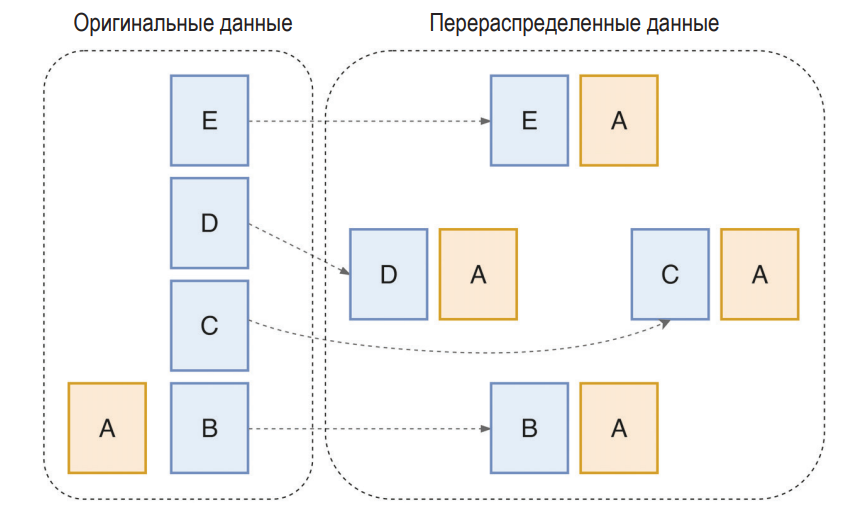
\includegraphics[scale=0.6]{figures/imbalanced_h4.png}
	\caption{ Ансамбль перераспределенных наборов данных }\label{fig:imbalanced_h4}
\end{figure}

Этот подход прост и хорошо масштабируется: мы можем обучить и выполнить модели на разных процессорных ядрах или узлах кластера. Кроме того, ансамбль моделей дает лучшие предсказания, чем каждая отдельная модель.

Тот же прием из книги Лакшманана \cite[\strbook{167}]{lakshmanan-mldp:2022}. Понижающий отбор также часто сочетается с паттерном <<Ансамбли>>. Используя этот подход, вместо полного удаления случайной выборки из мажоритарного класса мы используем разные его подмножества для тренировки нескольких моделей, а затем совмещаем эти модели. В целях иллюстрации предположим, что у нас есть набор данных со 100 примерами миноритарного класса и 1000 примерами мажоритарного класса. Вместо удаления 900 примеров из мажоритарного класса мы бы разбили мажоритарные примеры случайно на 10 групп по 100 примеров в каждой, чтобы идеально сбалансировать набор данных. Затем мы бы натренировали 10 классификаторов, каждый с теми же 100 примерами из миноритарного класса и 100 разными, случайно отобранными значениями из мажоритарного класса.

Про подбор порога бинаризации для классификатора. В дополнение к сочетанию подходов, которые делают акцент на данных, мы также можем корректировать порог классификатора, чтобы выполнять оптимизацию под метрики точности или полноты в зависимости от варианта использования. Если бы мы были больше заинтересованы в том, чтобы модель была правильной всякий раз, когда она делает предсказание положительного класса (другими словами, если бы мы хотели снизить число \emph{ошибок первого рода}, т.е. FP), мы бы оптимизировали предсказательный порог под метрику точности, так как точность -- это истинно-положительных экземпляров в группе экземпляров, которые классификатор посчитал положительными, и следовательно зависит от FP. Если же дороже обходится упущение потенцильной положительной классификации (ошибка второго рода, FN), даже если мы можем ошибаться, то мы оптимизируем нашу модель под метрику полноты.

Важное замечание про тестовый поднабор данных \cite[\strbook{156}]{lakshmanan-mldp:2022}. Независимо от того, как мы модифицируем набор данных для тренировки, мы должны оставлять тестовый набор как есть, чтобы он обеспечивал точное представление изначального набора данных. Другими словами, тестовый набор должен иметь примерно такой же баланс классов, как и изначальный набор данных. В приведенном примере это 5\% мошенничества и 95\% не мошенничества.

Понижающий отбор \cite[\strbook{157}]{lakshmanan-mldp:2022}. Пусть набор данных содержит 6,3 млн. примеров, из которых только 8 тыс. являюется мошенническими транзакциями. Это число составляет всего лишь 0,1\% всего набора данных. Хотя крупный набор данных нередко улучшает способность модели выявлять закономерности, он менее полезен, когда данные значительно несбалансированы. Мы можем решить эту проблему, удалив из набора данных большой кусок мажоритарного класса. Мы возьмем все 8 тыс. мошеннических примеров и отложим их в сторону, чтобы использовать во время тренировки модели. Затем возьмем небольшую случайную выборку не мошеннических транзакций. Далее мы объединим ее с 8 тыс. мошенническими примерами, перетасуем данные и применим этот новый, меньший набор данных для тренировки модели. После этого наш набор данных будет содержать мошеннических транзакций, являясь гораздо более сбалансированным, чем изначальный набор данных, в котором только 0.1\% приходится на миноритарный класс. При понижающем отборе неплохо поэкспериментировать с точным используемым балансом. Здесь мы использовали разбивку 25/75, но для достижения точности может потребоваться разбивка, более близкая к 50/50.

Понижающий отбор обычно сочетают с паттерном <<Ансамбли>>, соблюдая следующие шаги:
\begin{enumerate}
	\item Подвергнуть мажоритарный класс понижающему отбору и использовать все экземпляры миноритарного класса,
	
	\item Натренировать модель и добавить ее в ансамбль,
	
	\item Повторить.
\end{enumerate}

Во время предсказательного вывода следует брать \emph{медианное} значение на выходе из \emph{ансамблевых моделей}.

В статье Дьяконова прием подбора порога бинаризации классификатора описывается в следующем виде. Обычно модель получает некотрые оценки принадлежности к классам, а сама классификация -- это результат бинаризации (по умолчанию порог 0.5). Но порог можно подбирать. Простая стратегия: при скользящем контроле по 10 фолдам получим оценки принадлежности классу 1 \emph{на обучении} (функция \texttt{cross\_val\_predict(method="predict\_proba")}), потом для заданного функционала качества подберем оптимальный порог бинаризации (при котором значение функционала максимально). \emph{Этот же порог} будем потом использовать \emph{на тесте}.

\textbf{Выводы} по работе с несбалансированными наборами данных:
\begin{itemize}
	\item Если дисбаланс в наборе небольшой (грубо <<40 на 60>>) и признаки вещественные, то можно воспользоваться либо приемом обогащения миноритарного класса синтетическими экземплярами, сгенерированными с помощью техник SMOTE или ADASYN (!), либо можно ничего не делать с набором данных, а использовать ансамблевые методы на деревьях принятия решений (в этом случае неважно какие типы признаков участвуют в описании объекта -- вещественные, категориальные или еще какие-либо). <<Деревянные>> модели часто и без устранения дисбаланса неплохо работают. Для оценки производительности можно использовать гармоническое среднее, каппу Коэна, коэффициент Метьюса. Как правило, дисбаланс набора данных для <<деревянных>> моделей практически не влияет на значение этих метрик, а сами метрики слабо чувствительны как к взешиванию классов, так и к подбору порога бинаризации классификатора,
	
	\item Если дисбаланс значительный (скажем, <<20 на 80>>), то можно один \emph{сильно разбалансированный набор данных} представить в виде нескольких \emph{сбалансированных наборов данных}. Из мажоритарного класса случайным образом выбираются экземпляры без возвращения в количестве равном мощности миноритарного класса, а экземпляры миноритарного класса просто копируются для каждого такого поднабора мажоритарного класса. В итоге получается $ N $ идеально сбалансированных наборов, на каждом из которых можно обучить модель, а потом просто выдать агрегат прогнозов (мажоритарным голосованием, мягким голосованием, усреднением и т.д.); прогноз на тестовом поднаборе данных будет генерироваться как и в случае беггинга: каждое дерево ансамбля, выращенное на своем идеально сбалансированном наборе данных дает прогноз, затем эти прогнозы агрегируются,
	
	\item В случае очень сильного дисбаланса (грубо <<1 на 99>>) и если размер миноритарного класса позволяет (т.е. миноритарный класс имеет достаточное колчиство экземпляров для обучения и тестирования) можно просто удалить б\emph{о}льшую группу экземпляров в мажоритарном классе, а из случайных подвыборок мажоритарного класса сформировать наборы с менее серьезным дисбалансом. На каждом таком меньшем наборе данных обучаем модели, собираем их в ансамбль и агрегируем прогнозы.
\end{itemize}


\section{Метрики MAPE, SMAPE, WAPE, WMAPE etc.}

\subsection{MAPE}

Метрика MAPE (Mean Absolute Percentage Error) вычисляется как 
\begin{align*}
	MAPE = 100\% \, \dfrac{1}{n} \sum_{t=1}^{n} | 1 - \dfrac{F_t}{A_t} |,
\end{align*}
где $ A_t $ -- истинное значение, $ F_t $ -- прогноз.

Очевидно, что если $ A_t = 0, F_t \neq 0 $, значение в $ t $-ой точке будет бесконечным. При низких значениях $ A_t, F_t $ ошибка будет завышенной. Поэтому если $ A_t, F_t $ принимают нулевые или близкие к нулю значения, рекомендуется использовать WAPE / WMAPE.

\subsection{SMAPE}

Метрику SMAPE рекомендуется вычислять по формуле
\begin{align*}
	SMAPE = 100\% \, \dfrac{ \sum\limits_{t=1}^{n} | A_t - F_t |}{ \sum\limits_{t=1}^n A_t + F_t }
\end{align*}

Выходит, что симметричный вариант MAPE не симметричный, а вот обычная MAPE симметричная.



\subsection{WAPE / WMAPE}

Метрика WAPE (Weighted Average Percentage Error) вычисляется по формуле
\begin{align*}
	WAPE = 100\% \, \dfrac{ \sum\limits_{t=1}^{n} |A_t - F_t| }{ \sum\limits_{t=1}^{n} |A_t|}
\end{align*}
а метрика WMAPE (Weighted Mean Absolute Percentage Error) -- как
\begin{align*}
	WMAPE = 100\% \, \dfrac{ \sum\limits_{t=1}^{n} w_t |A_t - F_t| }{ \sum\limits_{t=1}^{n} w_t |A_t|}
\end{align*}
\begin{lstlisting}[
style = ironpython,
numbers = none
]
def weighted_mean_average_percentage_error(
    y_true: t.Iterable,
    y_pred: t.Iterable,
    *,
    weights: t.Optional[t.Iterable] = None
) -> float:
    """Calculates WAPE(weights is None) or WMAPE(weights is not None)"""
    if len(y_true) != len(y_pred):
        raise ValueError("Error! y_true.len must be equal to y_pred.len")
    else:
        if weights is not None and len(y_true) != len(weights):
            raise ValueError("Error! y_true.len or y_pred.len must be equal to weights.len")
    
    if weights is None:
        weights = np.ones_like(y_true)
    
    return 100 * (weights * np.abs(y_true - y_pred)).sum() / (weights * np.abs(y_true)).sum()
\end{lstlisting}



\section{Внедрение моделей машинного обучения в промышленную эксплуатацию}

\url{https://www.bigdataschool.ru/blog/mlops-deployment-patterns-and-strategies.html}

MLOps-энтузиасты выделяют следующие \emph{паттерны внедрения моделей машинного обучения в прод}
\begin{itemize}
	\item Модель как услуга или сервис (Model-as-Service),
	
	\item Модель как зависимость (Model-as-Dependency),
	
	\item Предварительный расчет (Precompute),
	
	\item Модель по запросу (Model-on-Demand),
	
	\item Гибридная модель обслуживания (Hybrid Model Serving) или Федеративное обучение (Federated Learning)
\end{itemize}

\subsection{Паттерны внедрения ML-моделей в промышленную эксплуатацию}

\url{https://ml-ops.org/content/three-levels-of-ml-software}

\subsubsection{Модель как услуга (Model-as-Service)}

Это весьма распространенный шаблон для предоставления модели машинного обучения в качестве независимой услуги. Обычно это реализуется через заключение ML-модели и интерпретатора в выделенную веб-службу, к которой приложения-потребители данных запрашивают через REST API или удаленный вызов процедур (RPC, Remote Procedure Call). Такой паттерн пригоден для различных рабочих процессов машинного обучения, от пакетного прогнозирования до онлайн-обучения модели в потоковом режиме (\pic{fig:ml_as_service}).

REST API \url{https://skillbox.ru/media/code/rest-api-chto-eto-takoe-i-kak-rabotaet/} -- архитектурный подход, который устанавливает ограничения для API: как они должны быть устроены и какие фукнции поддерживать. Это позволяет стандартизировать работу программных интерфейсов, сделать их более удобными и производительными.

В отличие от SOAP API, REST API -- не протокол, а простой список рекомендаций, которым можно следовать или не следовать. Поэтому у него нет собственных методов. С другой стороны, его автор Рой Финлдинг создал еще и протокол HTTP, так что они очень хорошо сочетаются, и REST обычно используют в связке с HTTP. Хотя REST -- это не только HTTP, а HTTP -- не только REST.

Всего в REST есть шесть требований к проектированию API. Пять из них обвязательные, одно -- опциональное:
\begin{itemize}
	\item Клиент-серверная модель (clinent-server model),
	
	\item Осутствие состояния (statelessness),
	
	\item Кэширование (cacheability),
	
	\item Удинообразие интерфейса (uniform interface),
	
	\item Многоуровневая система (layered system),
	
	\item Код по требованию (code on demand) -- необязательно.
\end{itemize}

В вебе ресурсами называют любые данные: текст, изображение, видео, аудио, программу и пр.

Так как REST -- архитектурный подход, а не протокол, в нем не заложено никаких конкретных методов. На чаще всего его применяют со стандартом HTTP, в котором заложены сосбвтенные методы.

Если кратко, то в HTTP прописан набор действий, который можно описать аббревиатурой CRUD: create, read, update, delete. Для каждого такого действестия существует один или несколько методов. Например, \verb|GET| для чтения, а \verb|PUT| или \verb|PATCH| -- для разных видов обнавления.

Итак:
\begin{itemize}
	\item REST -- это \emph{архитектурный стиль API}. Он не ограничивается никакими протоколами и не имеет собственных методов. Но обычно в RESTful-сервисах используют стандарт HTTP, а файлы передают в формате JSON или XML,
	
	\item Есть шесть приницпов, на которых строится REST: клиент-серверная модель, отсутствие состояния, кэширование, единообразие интерфейса, многоуровневая система, код по требованию. Последний из них необязателен,
	
	\item REST-подход к архитектуре позволяет сделать сервисы отказоустойчивыми, гибкими и производительными, а при их масштабировании и внесении изменений не возникает больших сложностей.
\end{itemize}

\begin{figure}[h]
	\centering
	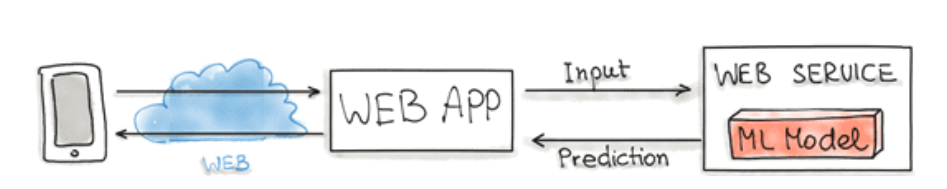
\includegraphics[scale=0.6]{figures/ml_as_service.png}
	\caption{ Машинное обучение как услуга -- самый простой шаблон MLPOps }\label{fig:ml_as_service}
\end{figure}

\subsubsection{Модель как зависимость (Model-as-Dependency)}

Это наиболее простой способ упаковать модель машинного обучения, которая рассматривается как зависимость внутри программного приложения. Например, приложение использует ML-модель как обычную зависимость от jar-файла, вызывая метод прогнозирования и передавая значения. Возвращаемые значения такого -метода -- некоторый прогноз, который выполняется предварительно обученной ML-моделью. Как правило, этот подход используется в задачах простого \emph{пакетного прогнозирования} (\pic{fig:ml_as_dependency}).

\begin{figure}[h]
	\centering
	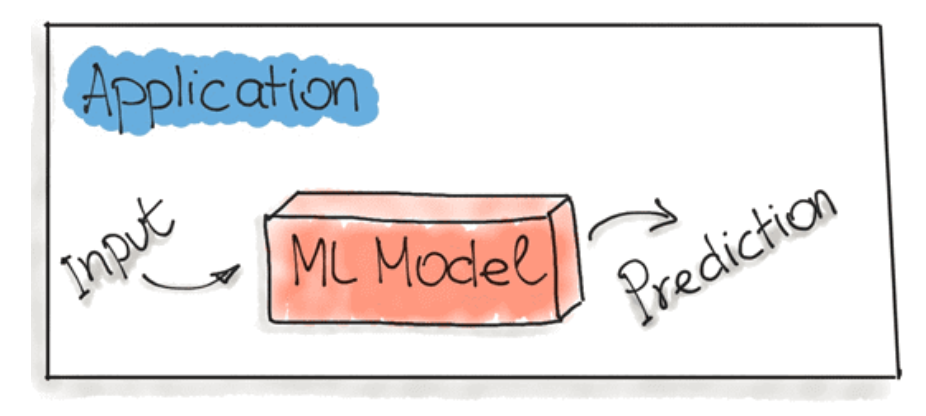
\includegraphics[scale=0.6]{figures/ml_as_dependency.png}
	\caption{ Модель как зависимость (Model-as-Dependency) }\label{fig:ml_as_dependency}
\end{figure}

\subsubsection{Предварительный расчет (Precompute)}

В этом случае прогнозы предварительно вычисляются с использованием уже обученной ML-модели для входящего пакета данных и сохраняются в базе. Далее к этой базе идет обращение при любом входном запросе, чтобы получить результат прогнозирования. С архитектурной точки зрения это похоже на Лямбда-шаблон, когда <<горячая>> обработка данных в потоковом режиме совмещается с <<холодной>>, где пакеты исторических данных подгружаются из хранилища, в качестве которого обычно выступает Data Lake на Apache Hadoop \pic{fig:precompute}.

 \begin{figure}[h]
 	\centering
 	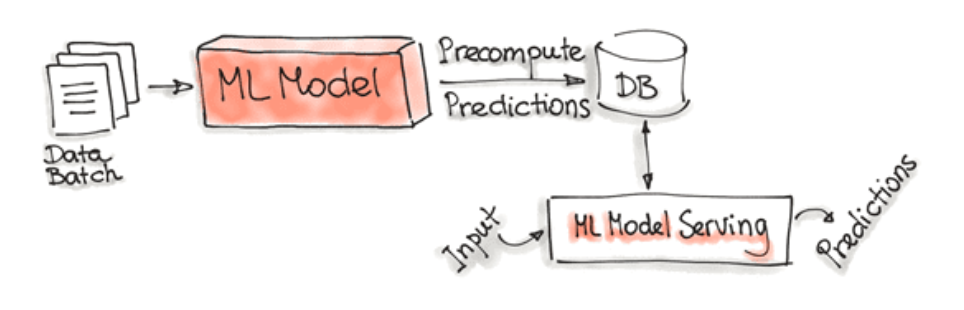
\includegraphics[scale=0.6]{figures/precompute.png}
 	\caption{ Лямбда-архитектура для ML-систем в MLOps (Precompute) }\label{fig:precompute}
 \end{figure}

\subsubsection{Модель по запросу (Model-on-Demand) с Apache Kafka}

Этот вариант рассматривает модель машинного обучения как зависимость, доступную во время выполнения. Однако, в отличие от паттерна <<Модель как зависимость>>, Model-on-Demand имеет собственный цикл выпуска и публикуется независимо. Для этой реализации обычно используется брокер сообщений, например, Apache Kafka или RabbitMQ. В этом случае применяется популярный в BigData \emph{подход потоковой обработки событий} (event-stream processing), когда \emph{данные} представляются в виде \emph{потока событий}, объединенные в канал.

Каналы событий представляют собой \emph{очереди сообщений}:
\begin{itemize}
	\item \emph{входную},
	
	\emph{выходную}
\end{itemize}

Брокер сообщений позволяет одному процессу записывать запросы на прогнозирование во входную очередь. Обработчик событий (event processor) содержит модель, обслуживающую среду выполнения, и ML-модель. Этот процесс подключается к брокеру, считывает из очереди запросы в пакетном режиме и отправляет их ML-модели для прогнозирования. Процесс обслуживания модели запускает генерацию прогнозов для входных данных и записывает полученные прогнозы в выходную очередь. Оттуда результаты прогнозирования отправляются в сервис, который инициировал запрос \pic{fig:model_on_demand}.

 \begin{figure}[h]
	\centering
	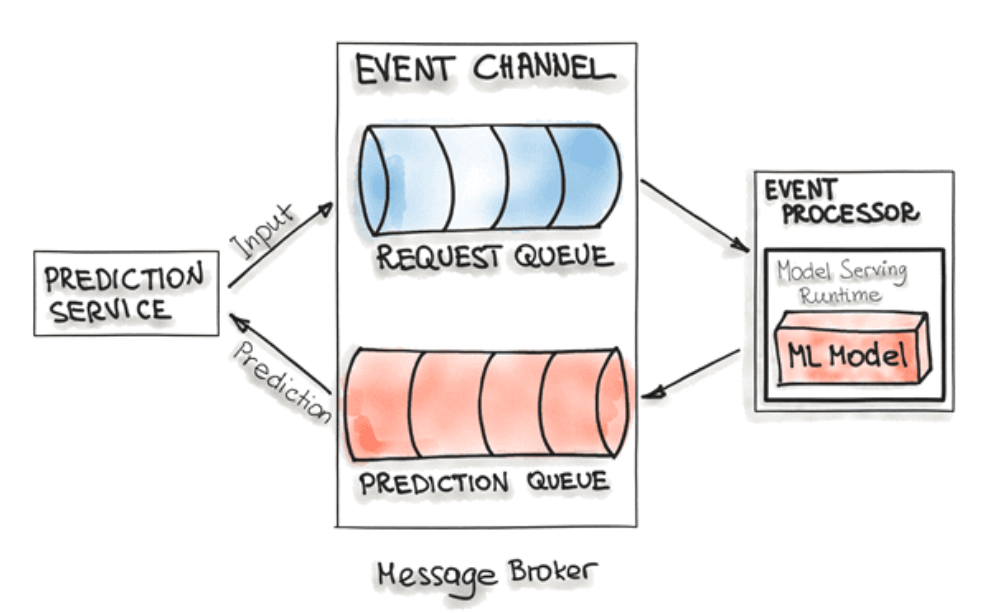
\includegraphics[scale=0.6]{figures/model_on_demand.png}
	\caption{ Модель по запросу (Model-on-Demand) }\label{fig:model_on_demand}
\end{figure}

\subsubsection{Гибридная модель обслуживания (Hybrid Model Serving)}

Уникальность федеративного обучения или гибридного обслуживания в том, что оно работает со множеством ML-моделей, индивидуальных для каждого пользователя в дополнение к той, которая храниться на сервере. Серверная модель обучается только один раз с реальными данными и выступает в качестве начального образца для каждого польозвателя. Далее она может видоизменяться в пользовательских вариациях, даже на мобильных устройствах, параметры которых сегодня позволяют обучать собственные ML-алгоритмы. Периодически пользовательские устройства отправляют на сервер уже обученные данные своей ML-модели, корректируя серверный вариант. Оттуда эти изменения могут быть распространены на остальных пользователей, с учетом предварительной проверки и тестирования на функциональность.

Главным плюсом такого гибридного подхода является то, что обучающие и тестовые данные, которые носят исключительно личный характер, никогда не покидают пользовательские устройства, сохраняя при этом все доступные данные. Это позволяет обучать высокоточные ML-модели без необходимости хранить гигабайты данных в облаке. Однако, стоит помнить, что обычные алгоритмы машинного обучения ориентированы на однородные большие данные, которые обрабатываются на мощном оборудовании и всегда доступны для обучения. Современные мобильные устройства поке еще менее мощные, чем специализированные Big Data кластера, а также обучающие данные распределены по миллионам устройств, которые не всгеда доступны. С учетом этого был создан отдельный фреймворк -- TensorFlow Federated, облегченная форма TensorFlow для федеративного обучения (\pic{fig:hybrid_model_serving}).

 \begin{figure}[h]
	\centering
	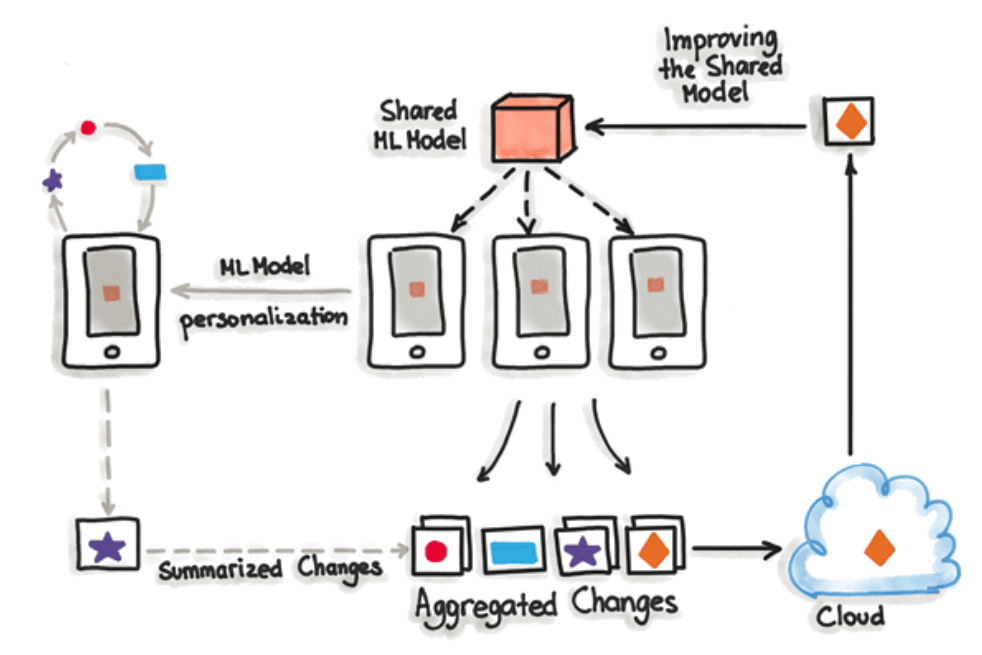
\includegraphics[scale=0.6]{figures/hybrid_model_serving.png}
	\caption{ Гибридная модель обслуживания или Федеративное обучение }\label{fig:hybrid_model_serving}
\end{figure}

\subsection{Стратегии внедрения ML-модели в прод}

\subsubsection{Развертывание с помщью Docker-контейнеров}

Этот вариант подходит для \emph{легковесных} ML-моделей \emph{без сохранения состояния}. В этом случае код модели машинного обучения заключен в Docker-контейнер, который считается наиболее распространенной технологией контейнеризации для локального, облачного или гибридного развертывания. Оркестрация таких контейнеров обычно выполняется с помощью Kubernetes или альтернатив, таких как AWS Fargate. Функциональные возможностит модели Machine Learning доступны через REST API, например, в виде приложения на Flask (\pic{fig:ml_model_docker_kube}).

 \begin{figure}[h]
	\centering
	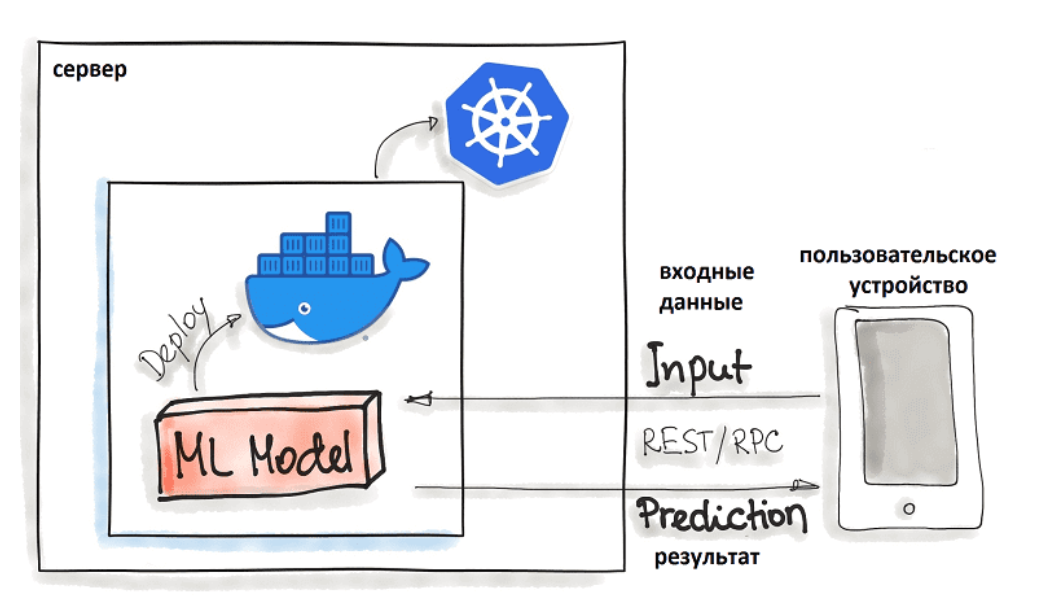
\includegraphics[scale=0.6]{figures/ml_model_docker_kube.png}
	\caption{ Развертывание ML-модели с помощью Docker и Kubernetes }\label{fig:ml_model_docker_kube}
\end{figure}

\subsubsection{Бессерверные вычисления (serverless)}

Код приложения и зависимости упаковываются в файлы \verb|.zip| с одной функцией точки входа. Затем этой функцией могут управлять основные облачные провайдеры, такие как Azure Functions, AWS Lambda или Google Cloud Functions. Однако следует обратить внимание на возможные ограничения развертываемых артефактов, в частности, их размеры. Напомним, servless-подход реализует PasS- или FaaS- (функция как услуга, Function-as-Service) стратегию, когда облако автоматически и динамически управляет выделением вычислительных ресурсов в зависимости от пользовательской нагрузки.

При этом для выполнения \emph{каждого запроса} (вызова функции) \emph{создается отдельный контейнер} или виртуальная машина, уничтожающиеся после выполнения. Преимуществом этого является избавление пользователей от работы по выделению и настройки серверов, в т.ч. виртуальных машин, контейнеров, баз данных, приложений, экземпляров сред выполнения. Все конфигурации и планирование вычислительных ресурсов для запуска кода по требованию или по событию скрыты от пользователей и управляются облаком. Бессерверный код может быть частью приложений, построенных на традиционной архитектуре, например, на микросервисах. Обратной стороной этих достоинств являются зависимость от облачного провайдера, сложность в поиске причин случившихся ошибок из-за многослойной инкапсуляции внутренненого устройства всей системы, а также время на запуск облачной функции, которое может быть критично для бизнеса \pic{fig:serverless}

 \begin{figure}[h]
	\centering
	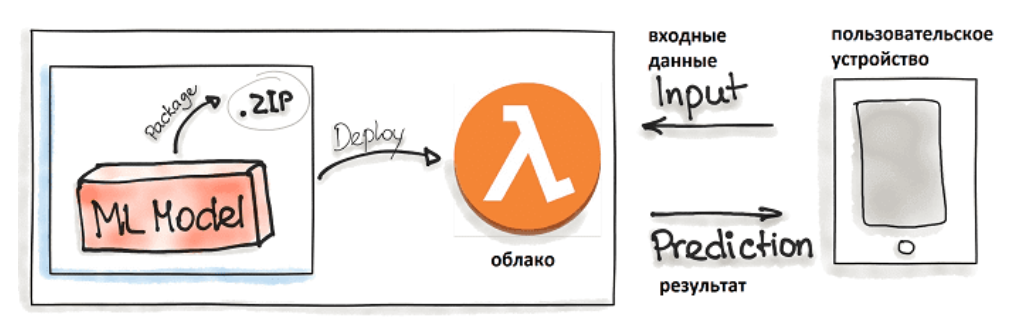
\includegraphics[scale=0.6]{figures/serverless.png}
	\caption{ Бессерверная стратегия внедрения ML-модели в прод }\label{fig:serverless}
\end{figure}






\section{ML System Design Doc}

Очень полезный шаблон для дорожной карты ML-продукта \url{https://github.com/IrinaGoloshchapova/ml_system_design_doc_ru}


\section{Квантильная регресия}

\url{https://scikit-learn.org/stable/modules/linear_model.html#quantile-regression}

Квантильная регрессия (модель линейной регрессии, которая предсказывает условные квантили) может быть полезна при построении интервальных, а не точечных оценок. Иногда интервальные прогнозы строятся в предположении о нормальном распределении ошибки с нулевым средним и постоянной дисперсией. Квантильная регрессия дает адекватные интервалы даже тогда, когда у ошибки непостоянная дисперсия или когда ошибка негауссовская. 

Как и линейная модель, квантильная регрессия дает линейные прогнозы $ \hat{x}(w, X) = X \, w $ для $ q $-ого квантиля, $ q \in (0, 1) $. Веса модели $ w $ находятся для следующей оптимизационной проблемы
\begin{align*}
	\min_w \dfrac{1}{ n_{samples} } \sum_i PB_q (y_i - X_i w) + \alpha \| w \|_1.
\end{align*}

То есть состоит из линейной потери (pinbal loss \url{https://scikit-learn.org/stable/modules/generated/sklearn.metrics.mean_pinball_loss.html#sklearn.metrics.mean_pinball_loss})
\begin{align*}
	PB_q(t) = q \, \max(t, 0) + (1 - q) \max(-t, 0) = 
	\begin{cases}
		qt, & t > 0,\\[-3mm]
		0, & t = 0, \\[-3mm]
		(q - 1)t, & t < 0
	\end{cases}
\end{align*}
и $ L_1 $-штрафа, как в модели Lasso.

Так как pinball loss линейна по остаткам, квантильная регрессия \emph{более устойчива к выбросам}, чем среднее на базе квадратической ошибки.

\section{MAE vs MSE. Устойчивость среднеабсолютной ошибки к выбросам}

Средняя абсолютная ошибка более устойчива к выбросам по сравнению с квадратической ошибкой. Потому что, оптимальным решением на классе константных алгоритмов для квадратической ошибки MSE является \emph{среднее арифметическое}, а для среднеабсолютной MAE -- \emph{медиана}.

Медиана, как известно, является более устойчивой к выбросам по сравнению со средним арифметическим. Несмотря на это, MSE обладает своими достоинствами -- в частности, для нее можно выписать аналитическое решение в случае линейной регрессии, а также ее можно оптимизировать напрямую при помощи градиентного спуска, в отличие от MAE, которая не является дифференциируемой по $ w $. 

\section{Оптимизационные задачи и теорема Куна-Таккера}

Рассмотрим задачу минимизации
\begin{align}\label{eq:opt_task}
\begin{cases}
	f_0 (x) \rightarrow \min\limits_{ x \in \mathbb{R}^d }\\
	f_i(x) \leqslant 0, \ i = 1, \ldots, m,\\
	h_i(x) = 0, \ i = 1, \ldots, p.
\end{cases}
\end{align}

Если ограничения в этой задаче отсутствуют, то имеет место \emph{необходимое условие экстремума}: если в точке $ x $ функция $ f_0 $  достигает своего минимума, то ее градиент в этой точке равен нулю. Значит, для решения задачи \emph{безусловной оптимизации} (нет ограничений)
\begin{align*}
	f_0(x) \rightarrow \min
\end{align*}
достаточно найти все решения уравнения
\begin{align*}
	\nabla f_0(x) = 0,
\end{align*}
и выбрать то, в котором достигается наименьшее значение. Для решения \emph{условных} задач оптимизации (в них есть ограничения) требуется более сложный подход.

Для задачи \eqref{eq:opt_task} можно записать \emph{лагранжиан} (функцию Лагранжа)
\begin{align*}
	L(x, \lambda, \nu) = f_0(x) + \sum_{i=1}^{m} \lambda_i f_i(x) + \sum_{i=1}^{p} \nu_i h_i(x), \ \lambda_i \geqslant 0,
\end{align*}
где $ \lambda_i, \nu_i $ -- \emph{множители Лагранжа} (двойственные переменные).

\emph{Двойственной функцией} для задачи \eqref{eq:opt_task} называется функция, получающаяся при взятии минимума лагранжиана по $ x $
\begin{align*}
	g(\lambda, \nu) = \inf_x L(x, \lambda, \nu).
\end{align*}

Двойственная функция дает \emph{нижнюю оценку} на \underline{минимум} в исходной оптимизационной задаче.

\emph{Условия Каруша-Куна-Таккера} (необходимые условия экстремума)
\begin{align*}
	\nabla f_0(x_*) + \sum_{i=1}^{m} \lambda_i^* \nabla f_i(x_*) + \sum_{i=1}^{p} \nu_i^* \nabla h_i (x_*) = 0\\
	f_i(x_*) \leqslant 0, \ i = 1, \ldots, m\\
	h_i(x_*) = 0, \ i = 1, \ldots, p\\
	\lambda_i^* \geqslant 0, \ i = 1, \ldots, m\\
	\lambda_i^* f_i(x_*) = 0, \ i = 1, \ldots, m
\end{align*}

Если задача \eqref{eq:opt_task} является выпуклой и удовлетворяет условию Слейтера, то условия Куна-Таккера становятся \emph{необходимыми} и \emph{достаточными}.


\section{Векторное дифференциирование}

Иногда при взятии производных по вектору или от вектор-функции удобно оперировать матричными операциями. Это упрощает запись и упрощает вывод формул.

Введем следующие определения:
\begin{itemize}
	\item При отображении вектора в число $ f(x): \mathbb{R}^n \rightarrow \mathbb{R} $ (то есть когда нужно взять производную от скалярной функции векторного аргумента $ f(x_1, \ldots, x_n) $ по каждому аргументу $ x_i $ в отдельности)
\begin{align*}
	\nabla_x f(x) = \Big[ \, \dfrac{ \partial f }{\partial x_1}, \ldots, \dfrac{ \partial f }{ \partial x_n } \, \Big]^T,
\end{align*}

    \item При отображении матрицы в число $ f(A): \mathbb{R}^{n \times m} \rightarrow \mathbb{R} $ (когда нужно взять производную функции от матрицы $ A $ по всем элементам матрицы $ A_{ij} $)
\begin{align*}
	\nabla_A f(A) = \Big( \dfrac{ \partial f }{ \partial A_{ij} } \Big)_{i, j = 1}^{n, m}.
\end{align*}
\end{itemize}

Мы хотим оценить, как функция изменяется по каждому из аргументов по отдельности. Поэтому производной от скалярной функции векторного аргумента по вектору будет \emph{вектор}, по матрице -- \emph{матрица}.

\remark{
Когда говорят, что нужно взять производную от скалярной функции векторного аргумента $ f(\underbrace{x_1, \ldots, x_n}_x) $ по вектору $ x $, это означает, что нужно взять производную от скалярной функции векторного аргумента $ f(x) $ по каждому элементу вектора $ x_i $. То есть запись $ \nabla_x f(x_1, \ldots, x_n) $ означает, частные производные $ \dfrac{\partial}{\partial x_i} $ от $ f(x) $. И аналогично, когда говорят, что нужно взять производную от функции матричного аргумента по матрице, это означает, что нужно взять производную функции матричного аргумента по каждому элементу матрицы. То есть запись $ \nabla_A f(A)$ означает частные производные по каждому элементу матрицы $ \dfrac{ \partial }{ \partial A_{ij} } $ от $ f(A) $
}

\emph{Задача 1}. Пусть $ a \in \mathbb{R}^n $ -- вектор параметров, а $ x \in \mathbb{R}^n $ -- вектор переменных. Необходимо найти производную их скалярного произведения по \emph{вектору переменных} $ \nabla_x a^T x $.

Так как $ a^T x $ это просто линейная комбинация переменных
\begin{align*}
	\dfrac{ \partial }{ \partial x_i } a^T x = \dfrac{ \partial }{ \partial x_i } \sum_j a_j x_j = a_i = \dfrac{ \partial f }{\partial x_i},
\end{align*}
то, собрав все $ n $ компонент $ \dfrac{ \partial f }{ \partial x_i } $ вместе, получим $ \nabla_x \underbrace{a^T x}_{f(x_1, \ldots, x_n)} = a $. То есть результатом будет вектор параметров $ a $.

Заметим, что $ a^T x $ -- это число, поэтому $ a^T x = (a^T x)^T = x^T a $, следовательно $\boxed{\nabla_x x^T a = \nabla_x a^T x = a} $.

\vspace*{3mm}\emph{Задача 2}. Пусть теперь $ A \in \mathbb{R}^{n \times n} $. Необходимо найти $ \nabla_x x^T A x $.
\begin{multline*}
	\dfrac{ \partial }{ \partial x_i } x^T A x = \dfrac{ \partial }{ \partial x_i } \sum_{j} x_j (A x)_j = \dfrac{ \partial }{ \partial x_i} \sum_{j} x_j \Big( \sum_k a_{jk} x_k \Big) = \dfrac{ \partial }{ \partial x_i } \sum_{j,k} a_{jk} x_j x_k = \\
	= \sum_{j \neq i} a_{ji} x_j + \sum_{k \neq i} a_{ik} x_k + 2 a_{ii} x_i = \sum_j a_{ji} x_j + \sum_k a_{ik} x_k = \sum_j (a_{ji} + a_{ij}) x_j.
\end{multline*}

Поэтому $ \boxed{\nabla_x x^T A x = (A + A^T) x} $.

\vspace*{3mm}\emph{Задача 3}. Пусть $ A \in \mathbb{R}^{n \times n} $. Необходимо найти $ \nabla_A \det A $. Воспользуемся теоремой Лапласа о разложении определителя по строке
\begin{align*}
	\dfrac{ \partial }{ \partial A_{\color{red}ij} } \det A = \dfrac{ \partial }{ \partial A_{ij} } \Big[ \sum_k (-1)^{i + k} A_{ik} M_{ik} \Big] = (-1)^{i + j} M_{\color{red}ij},
\end{align*}
где $ M_{ik} $ -- дополнительный минор\footnote{Дополнительным минором $ M_{ij} $ элемента $ a_{ij} $ называется определитель порядка $ n - 1 $, полученный из матрицы $ A $ порядка $ n $ вычеркиванием $ i $-ой строки и $ j $-ого столбца} матрицы $ A $. 

Элементы обратной матрицы
\begin{align*}
	(A^{-1})_{\color{red}ij} = \dfrac{1}{ \det A } (-1)^{i + j} M_{\color{red}ji}.
\end{align*}

Подставляя выражение для дополнительног минора, получаем ответ
\begin{align*}
	\boxed{\nabla_A \det A = (\det A) A^{-T}}
\end{align*}

Действительно, так как $ \det A (A^{-T})_{\color{red}ij}  = (-1)^{i + j} M_{\color{red}ij} $, то $ \dfrac{ \partial }{ \partial A_{ij} } \det A = \det A (A^{-T})_{ij} $.

\vspace*{3mm}\emph{Задача 4}. Пусть $ A \in \mathbb{R}^{n \times n}, B \in \mathbb{R}^{n \times n} $. Необходимо найти $ \nabla_A \text{tr} (AB) $.
\begin{align*}
	\dfrac{ \partial }{ \partial A_{ij} } \text{tr} (AB)  = \dfrac{ \partial }{ \partial A_{ij} } \sum_k (AB)_{kk} = \dfrac{ \partial }{ \partial A_{ij} } = \sum_{k,l} A_{kl}B_{lk} = B_{ji}.
\end{align*}

То есть $ \boxed{\nabla_A \text{tr} (AB) = B^T} $.

\vspace*{3mm}\emph{Задача 5}. Пусть $ x \in \mathbb{R}^n, A \in \mathbb{R}^{n \times m}, y \in \mathbb{R}^m $. Необходимо найти $ \nabla_A x^T A y $. Воспользоваться циклическим свойством следа матрицы (для матриц подходящего размера)
\begin{align*}
	\text{tr} (ABC) = \text{tr} (BCA) = \text{tr} (CAB)
\end{align*}
и результатом предыдущей задачи, получаем
\begin{align*}
	\nabla_A \underbrace{x^T A y}_{(1 \times 1)} = \nabla_A \text{tr} (x^T A y) = \nabla_A \text{tr} \big(  A \underbrace{(y x^T)}_B \big) = B^T = xy^T.
\end{align*}

\subsection{Решение задачи регрессии для многомерного случая}

В общем случае мы имеем выборку $ \{ (x_i, y_i)_{i=1}^l \},\ x_i \in \mathbb{R}^d, \ y \in \mathbb{R}, \ i = (1, \ldots, l) $ и мы хотим найти наилучшие парамемтры модели $ a(x) =  \langle w, x \rangle $ с точки зрения минимизации функции ошибки (то есть с точки зрения квадратической функции потерь)
\begin{align*}
	Q(w) = (y - X w)^T (y - X w).
\end{align*}

Здесь $ X \in \mathbb{R}^{l \times d} $ -- матрица <<объекты-признаки>> для обучающей выборки, $ y \in \mathbb{R}^l $ -- вектор значений целевой переменной на обучающей выборке, $ w \in \mathbb{R}^d $ -- вектор параметров.

Выпишем градиент функции ошибки по $ w $ (это просто скалярная функция векторного аргумента)
\begin{align*}
	\nabla_w Q(w) = \nabla_w [\, y^T y - y^T X w - w^T X^T y + w^T X^T X w \,] = 0 - X^T y - X^T y + (X^T X + X^T X) w = 0.
\end{align*}

Рассмотрим подробнее второй элемент в квадратных скобках $ \nabla_w \big(\underbrace{y^T}_{(1 \times l)} \underbrace{X}_{( l \times d )} \underbrace{w}_{( d \times 1)} \big) = \nabla_w \big( \underbrace{y^T X}_{(1 \times d)} \underbrace{w}_{( d \times 1)} \big) $. То есть в обозначениях $ \nabla_x a^T x = a $, $ y^T X = a^T $, а $ w = x $. Следовательно, здесь $ a = (y^T X)^T = X^T y $.

Аналогично для третьего элемента $ \nabla_w \big( w^T X^T y \big) $ в терминах $ \nabla_x x^T a = a $, элемент $ w^T = x^T $, а элемент $ X^T y = a $. То есть решением будет просто $ a = X^T y $.

Для четвертого элемента следует использовать формулу $ \nabla_x x^T A x = (A + A^T) x $.

Таким образом, искомый вектор параметров выражается так
\begin{align*}
	w = (X^T X)^{-1} X^T y.
\end{align*}

Покажем, что найденная точка -- точка минимума, если матрица $ X^T X $ обратима. Из курса матана мы знаем, что если матрица Гессе функции положительно определена в точке, градиент которой равен нулю, то эта точка является локальным минимумом (достаточное условие существования экстремума)

\begin{align*}
	\nabla_w^2 Q(w) = \nabla_w \big( 2X^T X\,w \big) = 2 X^T X \, \nabla_w w = \underbrace{2 X^T X}_{( d \times d )} \, \underbrace{E}_{(d \times d)} = 2 X^T X.
\end{align*}

Так как числовую матрицу соответствующих размеров можно выносить за знак производной.

Необходимо понять является ли матрица $ X^T X $ положительно определенной. Запишем определение положительной определенности матрицы $ X^T X $
\begin{align*}
	z^T X^T X z > 0, \forall z \in \mathbb{R}^d, \ z \neq 0.
\end{align*}

Видим, что тут записан квадрат нормы вектора $ X z $, то есть $ \| X z \|^2 \geqslant 0 $. В случае, если матрица $ X $ имеет книжную ориентацию (строк не меньше, чем столбцов) и имеет \emph{полный ранг}\footnote{Говорят, что у матрицы $ A \in \mathbb{R}^{n \times m} $ полный ранг, если $ \text{rg} A = \min(n, m) $} (нет линейно зависимых столбцов), то вектор $ X z $ не может быть нулевым, а значит выполняется
\begin{align*}
	z^T X^T X z = \| X z \|^2 > 0, \forall z \in \mathbb{R}^d, z \neq 0.
\end{align*}

Ранг матрицы равен наибольшему порядку отличного от нуля минора этой матрицы. 

То есть $ X^T X $ является положительно определенной матрицей. Если же строк оказывается меньше, чем столбцов, или $ X $ не является полноранговой (есть линейно зависимые столбцы), то $ X^T X $ \emph{необратима} ($ \det X^T X = 0 $) и решение $ w $ определено \emph{неоднозначно}.

\subsection{Градиентный спуск}

Ситуация, когда нам удается найти решение оптимизационной задачи в явном виде, -- большая удача. В общем случае оптимизационные задачи можно решать \emph{итерационно} с помощью \emph{градиентных методов} (или же методов, использующих как градиент, так и информацию о производных более высокого порядка).

\emph{Антиградиент} $ (- \nabla f(x_1, \ldots, x_n)) $ является направлением наискорейшего \underline{убывания} функции в заданной точке.

\section{Классические алгоритмы машинного обучения}

\subsection{Линейная регрессия}

Дано: коллекция размеченных данных $ \{ \mathbf{x}_i, y_i \}_{i=1}^N $, где $ N $ -- размер коллекции, $ \mathbf{x}_i $ -- D-мерный вектор признаков образца $ i = 1, \ldots, N $, $ y_i $ -- действительное целевое значение, и каждый признак $ x_i^{(j)}, j = 1, \ldots, D $ также является действительным числом.

Требуется: сконструировать модель $ f_\mathbf{w}, b (\mathbf{x}) $, являющуюся \emph{линейной комбинацией признаков экземпляра} $ \mathbf{x} $
\begin{align*}
	f_{ \mathbf{w}, b } (\mathbf{x})  = \mathbf{w} \mathbf{x} + b,
\end{align*}
где $ \mathbf{w} $ -- $ D $-мерный вектор параметров, $ b $ -- действительное число (смещение).

Запись $ f_{\mathbf{w}, b} $ означает, что модель параметризуется двумя значениями: $ \mathbf{w} $ и $ b $.

В линейной регрессии, в отличие от метода опорных векторов, \emph{гиперплоскость} проводится так, чтобы оказаться как можно ближе ко всем \emph{обучающим образцам}.

Чтобы удовлетворить это последнее требование (о прохождении гиперплоскости как можно ближе ко всем обучающим образцам), процедура оптимизации, используемая для поиска оптимальных значений $ \mathbf{x}^{*} $ и $ b^{*} $, должна \emph{минимизировать} следующее выражение \cite[\strbook{44}]{burkov:2020}
\begin{align*}
	\dfrac{1}{N} \sum_{i=1}^N \big( f_{\mathbf{w}, b} (\mathbf{x}_i) - y_i \big)^2.
\end{align*}

\remark{
Вместо квадартической функции потерь можно было использовать и функцию абсолютного отклонения, но последняя в отличие от квадратической функции потерь \emph{негладкая} (т.е. не имеет непрерывной производной) и потому создает лишние сложности, когда для поиска аналитических решений оптимизационных задач используются методы линейной алгебры.
}

Аналитические решения для нахождения оптимума функции -- это простые алгебраические выражения, и они часто предпочтительнее использования сложных \emph{численных методов оптимизации}, таких как \emph{градиентный спуск}.

Очевидно, что квадраты штрафов выгодны еще и потому, что преувеличивают разность между истинными и прогнозируемыми целевыми значениями, в соответствии с величиной этой разности.

\subsection{Логистическая регрессия}

Модель логистической регрессии
\begin{align*}
	f_{ \mathbf{w}, b } (\mathbf{x}) \mathrel{\stackrel{\rm def}=} \dfrac{1}{ 1 + e^{-( \mathbf{w} \mathbf{x} + b )} }
\end{align*}

То есть другими словами модель логистической регрессии представляет собой линейную комбинацию признаков, обернутую \emph{логистическим сигмоидом} $ \sigma(x) $, т.е.
$$
f_{ \mathbf{w}, b } (\mathbf{x}) = \sigma \Bigg( \sum_{i=1}^{N} w_i x_i + b \Bigg), \quad \sigma(x) = \dfrac{1}{ 1 + e^{-x} }.
$$

\remark{
В \emph{линейной регрессии} \underline{минимизируется} средне квадратическая ошибка (MSE), а в \emph{логистической регрессии} \underline{максимизируется} \emph{логарифм функции правдоподобия}
}

В статистике функция правдоподобия определяет, насколько правдоподобным выглядит наблюдение (образец) в соответствии с нашей моделью \cite[\strbook{48}]{burkov:2020}.

Критерий оптимизации в логистической регрессии называется максимальным правдоподобием. Вместо того чтобы минимизировать среднеквадратическую ошибку, как в линейной регрессии, мы теперь максимизируем правдоподобие обучающих данных в соотвествии с моделью
\begin{align*}
	L_{ \mathbf{w}, b } \mathrel{ \stackrel{\rm def} = } \prod_{i=1}^{N} f_{ \mathbf{w}, b } (\mathbf{x}_i)^{y_i} \, \big( 1 - f_{ \mathbf{w},b } (\mathbf{x}_i) \big)^{ (1 - y_i) }.
\end{align*}

Выражение $ f_{ \mathbf{w}, b } (\mathbf{x}_i)^{y_i} \, \big( 1 - f_{ \mathbf{w},b } (\mathbf{x}_i) \big)^{ (1 - y_i) } $ всего навсего означает, что <<$ f_{ \mathbf{w}, b } (\mathbf{x}_i) $, когда $ y_i = 1 $, и $ (1 - f_{ \mathbf{w},b } (\mathbf{x}_i)) $ иначе>>.

Таким образом, задача оптимизации в случае логистической регрессии имеет вид
\begin{align*}
	\argmin_{ \mathbf{w}, b } - \sum_{i=1}^N \Big[ y_i \ln f_{ \mathbf{w}, b } (\mathbf{x}) + (1 - y_i) \ln \big( 1 - f_{ \mathbf{w}, b } (\mathbf{x}_i) \big) \Big].
\end{align*}

В отличие от линейной регрессии, задача оптимизации выше не имеет аналитического решения. Поэтому в таких случаях обычно используется процедура численной оптимизации -- градиентный спуск.

\subsection{Деревья решений}

Дерево решений -- это ациклический граф, который можно использовать для принятия решений. В каждом ветвящемся узле графа исследуется $ j $-ый признак из вектор признаков. Если значение признака ниже определенного порога, то выбирается левая ветвь, а иначе -- правая. По достижении листового узла принимается решение о классе, к которому принадлежит образец.

В алгоритме \emph{ID3} качество расщипления оценивается с использованием энтропии. Энтропия достигает своего минимума, когда случайная величина может иметь только одно значение. И достигает своего максимума, когда все значения случайной величины равновероятны.

Алгоритм ID3 останавливается на листовом узле в любой из следующих ситуаций:
\begin{itemize}
	\item Все примеры в листовом узле правильно классифицируются моделью,
	
	\item Невозможно найти атрибут для расщипления,
	
	\item Расщипление уменьшает энтропию ниже некоторого значения $ \varepsilon $,
	
	\item Дерево достигает некоторой максимальной глубины $ d $.
\end{itemize}

Поскольку в ID3 решение о расщиплении набора данных в каждой итерации является локальным (не зависит от будущих расщиплений), алгоритм не гарантирует оптимального решения. Модель можно улучшить, использовав в процессе поиска оптимального дерева решений такие методы, как возврат, хотя и за счет увеличения времени построения модели.

Наиболее широко используемая версия алгоритма обучения дерева решений называется \emph{C4.5}. Версия алгоритма С4.5 имеет несколько дополнительных особенностей по сравнению с ID3 \cite[\strbook{54}]{burkov:2020}:
\begin{itemize}
	\item принимает непрерываные и дискретные признаки,
	
	\item поддерживает возможность обработки неполных данных,
	
	\item решает проблему переобучения с использованием восходящего метода, извсестного как <<подрезка>> (отсечение ветвей)ю
\end{itemize}

Подрезка заключается в том, чтобы выполнить обратный обход только что созданного дерева и удалить ветви, которые не вносят существенного вклада в уменьшение ошибки, заменив их листовыми узлами.

\subsection{Метод опорных векторов}

\subsubsection{Из документации scikit-learn}

\url{https://scikit-learn.org/stable/modules/svm.html#svm-classification}

\paragraph{Классификация с SVC. Общий случай}

Даны векторы $ x_i \in \mathbb{R}^p, i = 1, \ldots, n $ и целевой вектор $ y \in \{ +1, -1 \}^n $.

Наша цель заключается в том, чтобы найти такой вектор $ w \in \mathbb{R}^p $ и скаляр $ b \in \mathbb{R} $, что прогноз, вычисленный по формуле $ \text{sign}(w^T \varphi(x) + b) $, будет корректным для большинства экземпляров.

Прямая задача (primal problem)
\begin{align*}
	\min_{w, b, \zeta} \dfrac{1}{2} w^T w + C \sum_{i=1}^{n} \zeta_i \\
	y_i (w^T \varphi(x_i) + b) \geqslant 1 - \zeta_i \\
	\zeta_i \geqslant 0, i = 1, \ldots, n
\end{align*}

Интуитивно, мы пытаемся \emph{максимизировать зазор} (\emph{минимизируя квадрат эвклидовой нормы} $ \| w \|^2 = w^T w $). Параметр $ C $ управляет силой штрафа и действует как обратный параметр регуляризации.

\remark{
Гиперпараметр $ C $ связан с \emph{силой регуляризации} обратно пропорциональной зависимостью. То есть низким значениям параметра $ C $ отвечает сильная регуляризация (модель упрощается), а высоким значениям -- слабая регуляризация (модель усложняется)
}

Меньшее значение параметра $ C $ (что отвечает более сильной регуляризации $ \rightarrow $ модель упрощается) приводит к более широкой полосе, но б{\itshape о}льшему числу нарушений зазора \cite[\strbook{201}]{geron:hands_on_ml}

\paragraph{Классификация с LinearSVC. Случай линейного ядра}

Прямая задача
\begin{align*}
	\min_{w, b} \dfrac{1}{2} w^T w + C \sum_{i=1} \max[ \, 0, 1 - y_i (w^T \varphi(x_i) + b) \, ]
\end{align*}

Здесь используется \emph{кусочно-линейная функция потерь} (hing loss).

\paragraph{Регрессия с SVR. Общий случай}

Даны векторы $ x_i \in \mathbb{R}^p, i = 1, \ldots, n $ и целевой вектор $ y \in \mathbb{R}^n $. Прямая задача
\begin{align*}
	\min_{w, b, \zeta, \zeta^*} \dfrac{1}{2} w^T w + C \sum_{i=1}^n (\zeta_i + \zeta_i^*)\\
	y_i - (w^T \varphi(x_i) + b) \leqslant \varepsilon + \zeta_i, \\
	(w^T \varphi (x_i) + b) - y_i \leqslant \varepsilon + \zeta_i^*, \\
	\zeta_i, \zeta_i^* \geqslant 0, i = 1, \ldots, n
\end{align*}

\paragraph{Регрессия с LinearSVR. Случай линейного ядра}

Прямая задача
\begin{align*}
	\min_{w, b} \dfrac{1}{2} w^T w + C \sum_{i=1} \max [\, 0, |\, y_i - (w^T \varphi(x_i) + b) \,| - \varepsilon \,].
\end{align*}

Здесь используется \emph{функция потерь}, {\itshape не чувствительная к ошибкам в $ \varepsilon $-окрестности} (epsilon-insensitive loss).

\subsubsection{Из книги Жерона}

Методы SVM чувствительны к масштабам признаков: если масштаб, скажем по оси $ y $, будет значительно больше масштаба по оси $ x $ -- например, $ y = 0\ldots1000 $ против $ x = 1\ldots5 $, то б\emph{о}льший зазор получиться по оси $ y $. Дело в том, что методы SVM пытаются обеспечить самую широкую, какую только возможно, полосу между классами, так что если обучающий набор не масштабирован, то методы SVM, будут иметь тенденцию игнорировать небольшие признаки \cite[\strbook{602}]{geron:hands_on_ml} (\pic{fig:svm_scale}).

\begin{figure}[h]
	\centering
	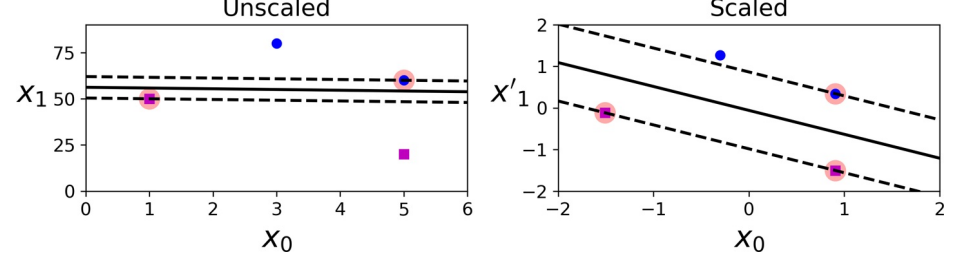
\includegraphics[scale=0.9]{figures/svm_scale.png}
	\caption{ Чувствительность к масштабам признаков. SVM посчитал горизонтальное положение полосы наиболее удачным, так как по оси $ x_1 $ масштаб больше и соответственно получается большее значении ширины зазаора }\label{fig:svm_scale}
\end{figure}

\emph{Классификация с жестким зазором} (hard margin classification) присущи две главные проблемы. Во-первых, она работает, только если данные \emph{линейно-сепарабельны}. Во-вторых, она довольно чувствительна к выбросам.

Чтобы избежать этих проблем, предпочтительнее применять более гибкую модель. Цель заключается в том, чтобы отыскать хороший баланс между удержанием полосы как можно более широкой и ограничением количества нарушений зазора. Это называется \emph{классификацией с мягким зазором} (soft margin classification)

В классах SVM библиотеки Scikit-Learn управлять упомянутым балансом можно с помощью параметра $ C $: меньшее значение $ C $ ведет к более широкой полосе, но большему числу нарушений зазора.

\verb|LinearSVC(C=1, loss="hinge")| похож на \verb|SVC(kernel="linear", C=1)| с точки зрения фунциональных возможностей, но основан на библиотеке liblinear\footnote{Библиотека liblinear реализует специальный алгоритм для \underline{\itshape линейных} методов SVM -- метод двойного покоординатного спуска (dual coordinate descent) \url{https://www.csie.ntu.edu.tw/~cjlin/papers/cddual.pdf}}, а не libsvm, работает гораздо быстрее и лучше масштабируется на большие выборки \cite[\strbook{202}]{geron:hands_on_ml}. Для улучшения производительности следует установить гиперпараметр \verb|dual| в \verb|False|. Флаг \verb|dual=True| означает, что будет решаться \emph{двойственная задача} (dual problem), а не \emph{прямая задача} (primal problem).

Рекомендуется (см.~\href{https://scikit-learn.org/stable/modules/generated/sklearn.svm.LinearSVC.html}{LinearSVC}) оптимизационную задачу решать в \emph{прямой} постановке (т.е. \verb|dual=False|), когда в матрице признакового описания объекта экезмпляров больше, чем признаков -- $ \text{n\_samples} > \text{n\_features} $ (книжная ориентация матрицы).

То есть оптимизационная задача для классификатора \verb|LinearSVC| может быть сформулирована как в \emph{прямой}, так и в \emph{двойственной} постановке.

\remark{
Ядерный трюк предотвращает комбинаторно бурный рост количества признаков, поскольку в действительности мы не добавляем никаких признаков
}

Класс \verb|LinearSVC| основан на библиотеке liblinear, не поддерживает ядерный трюк, но масштабируется почти линейно с ростом числа экземпляров $ m $ и числа признаков $ n $, а его временная сложность составляет $ \approx O(m \times n) $.

Класс \verb|SVC| основан на библиотеке libsvm и поддерживает ядерный трюк. Временная сложность обычно находится между $ O(m^2 \times n) $ и $ O(m^3 \times n) $. Это означает, что он становится невероятно медленным при большом количестве обучающих экземпляров (порядка нескольких сотен тысяч). Такой алгортим идеален для сложных, но небольших или средних обучающих наборов. Тем не менее, он хорошо масштабируется с ростом числа признаков, особенно разреженных.

Метод опорных векторов поддерживает не только \emph{линейную} и \emph{нелинейную} \underline{классификацию}, но и \emph{линейную} и \emph{нелинейную} \underline{регрессию}.

Регрессия SVM пытается уместить \emph{на полосе} как можно больше экземпляров наряду с ограничением нарушений зазора (т.е. экземпляров вне полосы) \cite[\strbook{210}]{geron:hands_on_ml}. Ширина полосы управляется гиперпараметром $ \varepsilon $ (\pic{fig:svm_linreg}).

\begin{figure}[h]
	\centering
	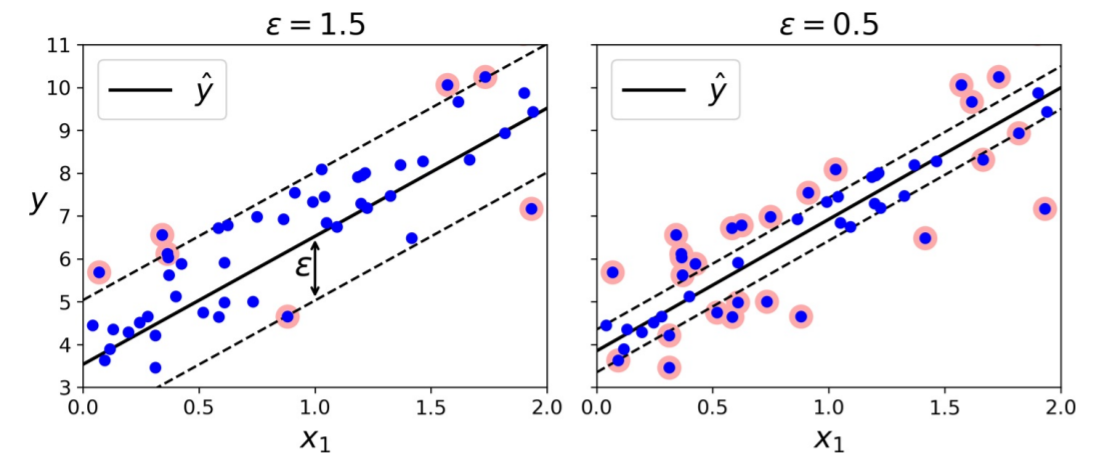
\includegraphics[scale=0.7]{figures/svm_linreg.png}
	\caption{ Линейная регрессия с помощью LinearSVR }\label{fig:svm_linreg}
\end{figure}

Добавление дополнительных обучающих экземпляров внутри зазора не влияет на прогнозы модели; потому говорят, что модель \emph{нечувствительна} к $ \varepsilon $.

Для решения задач \emph{линейной} регрессии можно использовать класс \verb|LinearSVR|, а для задач \emph{нелинейной} регрессии -- \verb|SVR|.

\begin{figure}[h]
	\centering
	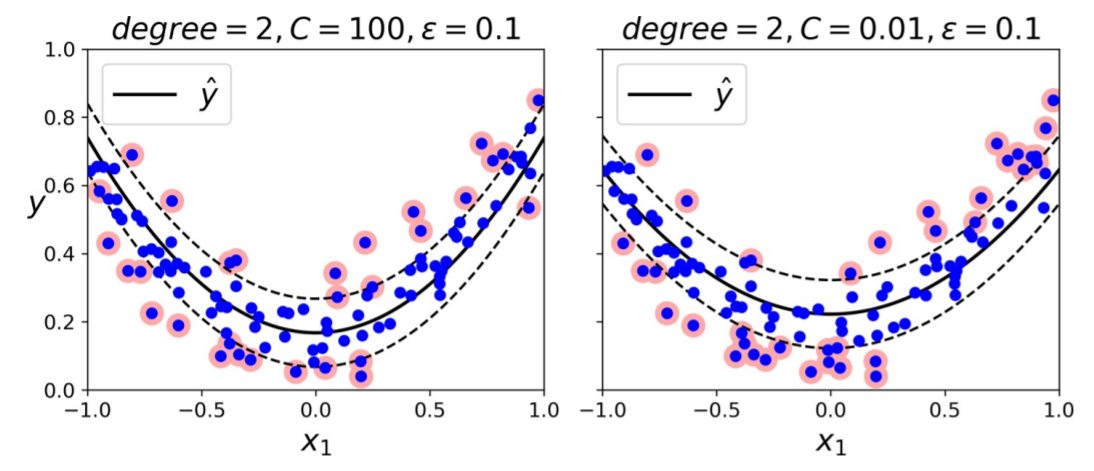
\includegraphics[scale=0.7]{figures/svm_nonlinreg.png}
	\caption{ Нелинейная регрессия с помощью SVR с полиномиальным ядром 2-ого порядка }\label{fig:svm_nonlinreg}
\end{figure}

\remark{
Класс SVR, как и SVC поддерживает ядерный трюк
}

Если в задаче $ n $ признаков, то \emph{функция решения}\footnote{decision function} -- это $ n $-мерная гиперплоскость (\pic{fig:svm_des_fun}), а \emph{граница решения}\footnote{decision boundary} (то есть множество точек, где функция решения равна нулю) -- это $ (n - 1) $-мерная гиперплоскость \cite[\strbook{212}]{geron:hands_on_ml}.

\begin{figure}[h]
	\centering
	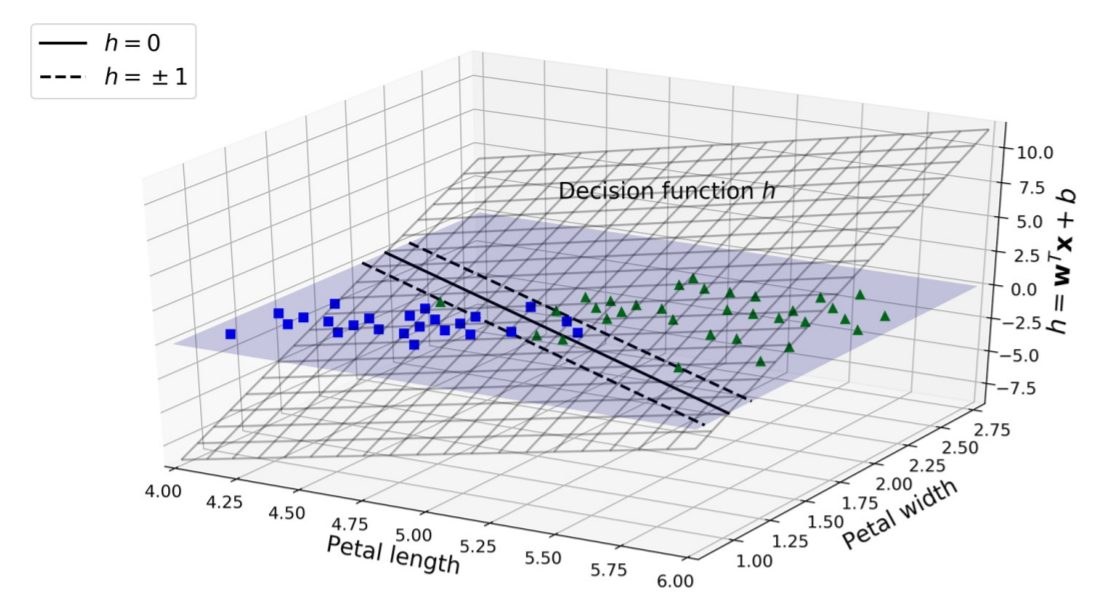
\includegraphics[scale=0.7]{figures/svm_des_fun.png}
	\caption{ Функция решения для набора данных об ирисах }\label{fig:svm_des_fun}
\end{figure}

Обучение линейного классификатора SVM означает нахождение таких значений $ \{w_1, \ldots, w_n\}, b $, которые делают \emph{зазор} как можно более \emph{широким}, одновременно \emph{избегая} нарушений зазора (жесткий зазор) или \emph{ограничивая} их (мягкий зазор) \cite[\strbook{213}]{geron:hands_on_ml}.

Задачи \emph{жесткого} и \emph{мягкого зазора} являются задачами выпуклой \emph{квадратичной} оптимизации с \emph{линейными} ограничениями \cite[\strbook{215}]{geron:hands_on_ml}. Такие задачи известны как задачи квадратичного программирования (Quadratic Programming -- QP).

То есть перейдя от оригинальной задачи (\emph{прямая задача}) с помощью метода множителей Лагранжа и записав условия Каруша-Куна-Таккера, приходим к \emph{двойственной задаче} и решаем ее (находим множители Лагранжа) методами квадратичного программирования.

Двойственная задача решается быстрее прямой, когда количество обучающих экземпляров меньше количества признаков. Но что более важно, в случае двойственной задачи становится возможен ядерный трюк, в то время как при решении прямой задачи он невозможен.

Ядро -- это функция, которая способна вычислять скалярное произведение $ \varphi(\mathbf{a})^T \cdot \varphi (\mathbf{b}) $, базируясь только на исходных векторах $ \mathbf{a} $ и $ \mathbf{b} $, без необходимости вычислять трансформацию $ \varphi $ (или даже знать о ней) \cite[\strbook{218}]{geron:hands_on_ml}.

\subsubsection{Из курса лекций Соколова}

Вспомним, что метод опорных векторов сводится к решению задачи оптимизации (для общего случая \emph{классификации} с мягким зазором с помощью SVC)
\begin{align*}
	\begin{cases}
		\dfrac{1}{2} \| w \|^2 + C \sum\limits_{i=1}^{l} \xi_i \to \min\limits_{ w, b, \xi }\\
		y_i ( \langle w, x_i \rangle + b) \geqslant 1 - \xi_i, \ i = 1, \ldots, l,\\
		\xi_i \geqslant 0, \ i = 1, \ldots, l.
	\end{cases}
\end{align*}

Построим \emph{двойственную} к ней. Запишем \emph{лагранжиан} (ограничения\footnote{Ограничения должны быть сведены к виду $ left\_part \geqslant 0 $} просто суммируются с учетом множителей Лагранжа $ \lambda_i, \mu_i $ и вычитаются из целевой функции)
\begin{align*}
	L(w, b, \xi, \lambda, \mu) = \dfrac{1}{2} \| w \|^2 + C \sum_{i=1}^{l} \xi_i - \sum_{i=1}^{l} \lambda_i [\, y_i (\langle w, x_i \rangle + b) - 1 + \xi_i \,] - \sum_{i=1}^{l} \mu_i \xi_i.
\end{align*}

Выпишем условия Каруша-Куна-Таккера
\begin{align}
	\nabla_w L = w - \sum_{i=1}^{l} \lambda_i y_i x_i = 0 \qquad &\Rightarrow w = \sum_{i=1}^{l} \lambda_i y_i x_i \label{eq:w}\\
	\nabla_b L = - \sum_{i=1}^l \lambda_i y_i = 0 \qquad &\Rightarrow \sum_{i=1}^l \lambda_i y_i = 0 \\
	\nabla_{\xi_i} L = C - \lambda_i - \mu_i \qquad &\Rightarrow \lambda_i + \mu_i = C \\
	\lambda_i [\, y_i ( \langle w, x_i \rangle + b) - 1 + \xi_i \,] = 0 \qquad &\Rightarrow (\lambda_i = 0) \ \text{или} \ (y_i ( \langle w, x_i \rangle + b ) = 1 - \xi_i) \label{eq:xi} \\
	\mu_i \xi_i = 0 \qquad &\Rightarrow (\mu_i = 0) \  \text{или} \ (\xi_i = 0) \\
	\xi_i \geqslant 0, \lambda_i \geqslant 0, \mu_i \geqslant 0.
\end{align}

При вычислении градиентов $ \nabla_w, \nabla_b, \nabla_{\xi_i} $ просто берем частные производные от лагранжиана $ L $ по каждому элементу $ w_1, w_2, \ldots $ вектора $ w $, по каждому элементу $ b_1, b_2, \ldots $ вектора $ b $ и т.д.

Проанализируем полученные условия. Из \eqref{eq:w} следует, что вектор весов $ w $, полученный в результате настройки SVM, можно записать как линейную комбинацию объектов $ x_i $ из объектов обучающей выборки, причем веса в этой линейной комбинации можно найти как решение двойственной задачи.

В зависимости от значений $ \xi_i $ и $ \lambda_i $ объекты $ x_i $ разбиваются на три категории:
\begin{enumerate}
	\item $ \xi_i = 0, \lambda_i = 0 $: такие объекты не влияют на решение $ w $ (входят в него с нулевым весом $ \lambda_i $), правильно классифицируются ($ \xi_i = 0 $) и лежат вне разделяющей полосы. Объекты этой категории называются \emph{периферийными}.
	
	\item $ \xi_i = 0, 0 < \lambda_i < C $: из условия \eqref{eq:xi} следует, что $ y_i ( \langle w, x_i \rangle + b ) = 1 $, то есть объект лежит \emph{строго на границе разделяющей полосы}. Поскольку $ \lambda_i > 0 $, объект влияет на решение $ w $. Объекты этой категории называются \emph{опорными граничными}.
	
	\item $ \xi_i > 0, \lambda_i = C $: такие объекты могут лежать внутри разделяющей полосы ($ 0 < \xi_i < 2 $) или выходить за ее пределы ($ \xi_i \geqslant 2 $). При этом если $ 0 < \xi_i < 1 $, то объект классифицируется правильно, в противном случае неправильно. Объекты этой категории называются \emph{опорными нарушителями}.
\end{enumerate}

Итак, итоговый классификатор зависит от объектов, лежащих на границе разделяющей полосы, и от объектов-нарушителей (c $ \xi_i > 0 $).

Приходим к следующей \emph{двойственной задаче}
\begin{align*}
	\begin{cases}
	    \sum\limits_{i=1}^{l} \lambda_i - \dfrac{1}{2} \sum\limits_{i,j=1}^{l} \lambda_i \lambda_j y_i y_j \langle x_i, x_j \rangle \to \max\limits_\lambda \\
	    0 \leqslant \lambda_i \leqslant C, \ i = 1, \ldots, l, \\
	    \sum\limits_{i=1}^{l} \lambda_i y_i = 0.
	\end{cases}
\end{align*}

\noindent Она также является вогнутой, квадратичной и имеет единственный максимум.

Двойственная задача SVM зависит только от скалярных произведений объектов -- отдельные признаковые описания никак в нее не входят. Значит, можно легко сделать ядровый переход
\begin{align*}
	\begin{cases}
		\sum\limits_{i=1}^l \lambda_i - \dfrac{1}{2} \sum\limits_{i,j=1}^l \lambda_i \lambda_j y_i y_j K(x_i, x_j) \to \max\limits_\lambda \\
		0 \leqslant \lambda_i \leqslant C, \ i = 1, \ldots, l, \\
		\sum\limits_{i=1}^l \lambda_i y_i = 0.
	\end{cases}
\end{align*}

Подставляя представление \eqref{eq:w} в классификатор, получаем
\begin{align*}
	a({\color{blue}x}) = \text{sign} \Big( \sum_{i=1}^l \lambda_i y_i \langle x_i, {\color{blue}x} \rangle + b \Big).
\end{align*}

Таким образом, {\color{blue}классификатор измеряет \emph{сходство} \underline{нового объекта} с \underline{объектами из обучающей выборки}, вычисляя \emph{скалярное произведение} между ними}. Это выражение также зависит только от скалярных произведений, поэтому в нем тоже можно сделать переход к ядру.

Если использовть гауссовское ядро (радиальную базисную функцию) в \emph{методе опорных векторов}, то получится следующее \emph{решающее правило}
\begin{align*}
	a({\color{blue}x}) = \text{sign} \sum_{i=1}^l y_i \lambda_i \underbrace{\exp \Bigg( - \dfrac{ \| {\color{blue}x} - x_i \|^2 }{ 2 \sigma^2 } \Bigg)}_{K(x, x_i)}
\end{align*}

То есть мы просто в решающем правиле заменили \emph{скалярное произведение} $ \langle x_i, x \rangle $ на \emph{ядро} $ K(x, x_i) $.

\subsubsection{Из книги Буркова}

После обучения алгоритм метода опорных векторов будет определяться так
\begin{align*}
	f(\mathbf{x}) = \text{sign} (\mathbf{w}^* \mathbf{x} - b^*)
\end{align*}

Чтобы с помощью модели метода опорных векторов предсказать, является ли электронное письмо спамом или нет, нужно взять текст письма, преобразовать его в вектор признаков, затем умножить этот вектор на $ \mathbf{w}^{*} $, вычесть $ b^{*} $ и взять знак результата. Это даст прогноз (+1 означает <<спам>>, а -1 означает <<не спам>>).

Но как машина находит $ \mathbf{w}^{*} $ и $ b^{*} $? Она решает задачу оптимизации. Машины хорошо справляются с оптимизацией функций в условиях ограничений.

Итак, какие ограничения должны удовлетворяться здесь? Прежде всего, модель должна правильно предсказывать метки имеющихся 10 000 данных. Каждый образец задается парой $ (\mathbf{x}_i, y_i) $, где $ \mathbf{x}_i $ -- вектор признаков $ i $-го образца, а $ y_i $ -- его метка, которая принимает значение -1 или +1. Ограничения выглядят следующим образом \cite{burkov:2020} 
\begin{align*}
	\mathbf{w} \mathbf{x}_i + b\geqslant +1, \text{если} \ y_i = +1,\\
	\mathbf{w} \mathbf{x}_i + b\leqslant -1, \text{если} \ y_i = -1.
\end{align*}

Желательно также, чтобы гиперплоскость отделяла положительные данные от отрицательных с максимальным зазором. Зазор -- это расстояние между ближайшими образцами двух классов ,отделяемых границей принятия решения.

Большой зазор способствует  лучшему обобщению, то есть тому, насколько хорошо модель будет классифицировать новые данные.

Для \emph{максимизации зазора} нужно \emph{минимизировать эвклидову норму} $ \| \mathbf{w} \| = \sqrt{ \sum\limits_{j=1}^D (w^{(j)})^2 }$ \cite[\strbook{23}]{burkov:2020}, так как расстояние между границами определяется как $ \dfrac{2}{ \| \mathbf{w} \| } $.

{В методе опорных векторов решается следующая задача \emph{оптимизации}: минимизировать эвклидову норму  $ \| \mathbf{w} \| $ с учетом $ y_i (\mathbf{w} \mathbf{x}_i - b) \geqslant 1, \ i = 1, \ldots, N $}

Рассмотренная версия алгоритма строит \emph{линейную модель} (граница принятия решения -- это прямая линия, плоскость или гиперплоскость). Однако метод опорных векторов также может включать \emph{ядра}, способные сделать границу решения \emph{произвольно нелинейной}.

\remark{
\emph{Градиент} -- обобщение понятия производной на случай скалярной функции векторного аргумента. Другими словами градиент -- вектор частных производных
}

В некотрых случаях невозможно полностью разделить две группы точек из-за шума в данных, ошибок разметки или аномалий (данных, сильно отличающихся от <<типичного>> образца в наборе данных). Для таких случаев есть версия алгоритма SVM, способная включить гиперпараметр штрафа за неправильную классификацию обучающих данных конкретных классов.

\remark{
Для того чтобы понять связь между ошибкой модели, размером обучающего набора, формой математического уравнения, определяющего модель, и временем построения модели, следует прочитать о \emph{вероятностно-приблизительное корректном обучении} (Probably Approximately Correct, PAC). Теория вероятностно-приблизительного корректного обучения поможет проанализировать и понять, сможет ли и при каких условиях алгоритм обучения получить приблизительно корректный классификатор 
}

Минимизация $ \| w \| $ эквивалентна минимизации $ \dfrac{1}{2} \| w \|^2 $. Тогда оптимизационную задачу для метода опорных векторов можно переписать так (алгоритм метода опорных векторов с \underline{жестким зазором}\footnote{hard-margin SVM})
\begin{align}\label{eq:svm_hard_margin}
	\min \dfrac{1}{2} \| w \|^2,\ \text{такое, что}\ y_i (\mathbf{x}_i \mathbf{w} - b) - 1\geqslant 0, \ i = 1,\ldots, N.
\end{align}

Чтобы распространить SVM на случаи, когда данные невозможно разделить линейно, введем \emph{кусочно-линейную функцию потерь} (hinge loss function): $ \max (0; 1 - y_i (\mathbf{w} \mathbf{x}_i - b)) $.

Кусочно-линейная функция потерь равна нулю, если прогноз $ \mathbf{w} \mathbf{x}_i $ лежит с правильной стороны от границы решения, так как в этом случае правая часть кусочно-линейной функции потерь будет отрицательна. Для данных, лежащих с неправильной стороны, значение функции пропорционально расстоянию от границ решения.

Алгоритм метода опорных векторов, оптимизирующий кусочно-линейную функцию потерь, называют методом опорных векторов с \underline{мягким зазором} (soft-margin SVM)
\begin{align*}
	\| \mathbf{w} \|^2 + C \dfrac{1}{N} \sum_{i=1}^N \max \big(0; 1 - y_i (\mathbf{w} \mathbf{x}_i - b)\big),
\end{align*}
где $ C $ -- гиперпараметр, определяющий компромисс между увеличением размера границы решения и гарантией местонахождения каждого $ \mathbf{x}_i $ с правильной стороны от границы решения.

SVM можно адаптировать для работы с наборами данных, которые нельзя разделять гиперплоскостью в исходном пространстве. Действительно, если удастся преобразовать исходное пространство в пространство более высокой размерности, можно надеяться, что данные станут линейно сепарабельны в этом преобразованом пространстве.

Использование функции для \underline{неявного} преобразования исходного пространства в пространство более высокой размерности в ходе оптимизации функции стоимости в SVM называется \emph{ядерным трюком} (kernel trick).

Чтобы понять, как работают ядра, прежде нужно посмотреть, как алгоритм оптимизации для SVM находит оптимальные значения для $ \mathbf{w} $ и $ b $.

Для решения задачи оптимизации \eqref{eq:svm_hard_margin} традиционно используется \emph{метод множителей Лагранжа}. Вместо оригинальной задачи проще решить эквивалентную задачу, сформулированную так
\begin{align*}
	\max_{ \alpha_1, \ldots, \alpha_N } \sum_{i=1}^N \alpha_i - \dfrac{1}{2} \sum_{i=1}^{N} \sum_{i=1}^N y_i \alpha_i (\mathbf{x}_i \mathbf{x}_k) y_k \alpha_k\ \text{при условии, что} \ \sum_{i=1}^N \alpha_i y_i = 0\ \text{и} \ \alpha_i \geqslant 0, i = 1, \ldots, N,
\end{align*}
где $ \alpha_i $ называются множителями Лагранжа.

В такой формулировке задача оптимизации превращается в выпуклую задачу квадратичной оптимизации, которая эффективно решается применением алгоритмов квадратичного программирования.

Чтобы преобразовать \emph{исходное векторное пространство} в \emph{пространство с большим числом измерений}, нужно преобразовать $ \mathbf{x}_i $ в $ \varphi( \mathbf{x}_i ) $ и $ \mathbf{x}_k $ в $ \varphi( \mathbf{x}_k ) $, а затем перемножить $ \varphi( \mathbf{x}_i ) $ и $ \varphi( \mathbf{x}_k ) $. Эти вычисления могут оказаться очень дорогостоящими.

С другой стороны, нас интересует только результат скалярного произведения $ \mathbf{x}_i \mathbf{x}_k $, который, как мы знаем, является действительным числом. Нам все равно, как будет получено это число, лишь бы оно было верным. Используя функцию ядра, можно избавиться от дорогостоящего преобразования исходных векторов признаков в векторы с более высокой размерностью и избежать необходимости вычислять их скалярное произведение. Мы заменим эти вычисления простой операцией с исходными векторами признаков, которая даст тот же результат.

Например, вместо преобразования $ (q_1, p_1) \to (q_1^2, \sqrt{2} q_1 p_1, ;p_1^2) $ и $ (q_1, p_2) \to (q_2^2, \sqrt{2} q_2 p_2, p_2^2) $ и последующего вычисления скалярного произведения $ (q_1^2, \sqrt{2} q_1 p_1, p_1^2) $ и $ (q_2^2, \sqrt{2} q_2 p_2, p_2^2) $, чтобы получить $ (q_1^2 q_2^2 + 2 q_1 q_2 p_1 p_2 + p_1^2 p_2^2) $, можно найти скалярное прозведение $ (q_1, p_1) $ и $ (q_2, p_2) $, чтобы получить $ (q_1 q_2 + p_1 p_2) $, а затем возвести в квадрат, чтобы получить тот же результат $ (q_1^2 q_2^2 + 2 q_1 q_2 p_1 p_2 + p_1^2 p_2^2) $.

Это был пример функции ядра, и мы использовали квадратичное ядро $ k( \mathbf{x}_i \mathbf{x}_k )  \mathrel{ \stackrel{\rm def}{=} ( \mathbf{x}_i \mathbf{x}_k )^2 } $.

Существует несколько функций ядра, из которых наиболее широко используется \emph{радиальная базисная функция} (гауссово ядро, RBF)
\begin{align*}
	k( \mathbf{x}, \mathbf{x}^{'} ) = \exp \Big( - \dfrac{ \| \mathbf{x} - \mathbf{x}^{'} \|^2 }{ 2 \sigma^2 } \Big),
\end{align*}
где $ \| \mathbf{x} - \mathbf{x}^{'} \|^2 $ -- квадрат евклидова расстояния между двумя векторами признаков.

Евклидово расстояние определяется следующим уравнением
\begin{align*}
	d( \mathbf{x}_i, \mathbf{x}_k ) \mathrel{ \stackrel{\rm def}{=} } \sqrt{ \sum_{j=1}^D \big( x_i^{(j)} - x_k^{(j)} \big)^2 }.
\end{align*}

\subsection{Метод k ближайших соседей}

Метод k ближайших соседей -- это непараметрический алгоритм обучения. В отличие от други алгоритмов обучения, позволяющих отбрасывать обучающие данные после построения модели, метод kNN сохраняет все обучающие экземпляры в памяти. Когда появится новый, ранее не встречавшийся образец, алгоритм kNN находит $ k $ обучающих данных, наиболее близких к $ \mathbf{x} $, и возвращает наиболее часто встречающуюся метку в случае классификации или среднее значение метки в случае регрессии.

Близость двух экземпляров данных определяется функцией расстояния. Нередко используется \emph{косинусное сходство}
\begin{align*}
	s( \mathbf{x}_i, \mathbf{x}_k ) \mathrel{ \stackrel{\rm def}{=} } \dfrac{ \sum\limits_{j=1}^D x_i^{(j)} x_k^{(j)} }{ \sqrt{ \sum\limits_{j=1}^D \big( x_i^{(j)} \big)^2 } \sqrt{ \sum\limits_{j=1}^D \big( x_k^{(j)} \big)^2 } },
\end{align*}
которая является мерой сходства двух векторов.

\subsection{Многослойный персептрон}

Нейронная сеть, так же как модель регрессии или SVM, -- это всего лишь математическая функция $ y = f_{NN}(\mathbf{x}) $. Функция $ f_{NN} $ имеет особую форму: это вложенная функция (вроде матрешки). Например, для трехслойной нейронной сети, возвращающей скаляр, $ f_{NN} $ выглядит так \cite[\strbook{91}]{burkov:2020}
\begin{align*}
	y = f_{NN}(\mathbf{x}) = f_3(\mathbf{f}_2(\mathbf{f}_1(\mathbf{x}))),
\end{align*}
где $ \mathbf{f}_1 $ и $ \mathbf{f}_2 $ в уравнении выше -- это векторные функции, которые определяются как
\begin{align*}
	\mathbf{f}_l (\mathbf{z}) \mathrel{\stackrel{\rm def }=} \mathbf{g}_l (\mathbf{W}_l \mathbf{z} + \mathbf{b}_l),
\end{align*}
где $ l $ -- это индекс слоя и может охватывать от 1 до любого количества слоев; $ \mathbf{g}_l $ -- функция активации.

Параметры $ \mathbf{W}_l $ (матрица) и $ \mathbf{b}_l $ (вектор) определяются для каждого слоя в ходе обучения, с использованием градиентного спуска для оптимизации.

Важный момент: здесь вместо вектора $ \mathbf{w}_l $ используется матрица $ \mathbf{W}_l $. Причина в том, что $ \mathbf{g}_l $ -- векторная функция. Каждая строка $ \mathbf{w}_{l, u} $ ($ u $ означает <<узел>>) в матрице $ \mathbf{W}_l $ является вектором той же размерности, что и $ \mathbf{z} $.

Пусть $ a_{l, u} = \mathbf{w}_{l, u} \mathbf{z} + b_{l, u} $. На выходе $ \mathbf{f}_l(\mathbf(z)) $ возвращает вектор $ \{ g_l(a_{l,1}), g(a_{l,2}), \ldots, g_l(a_{l, size_l}) \} $, где $ g_l $ -- некоторая скалярная функция (возвращает скаляр, а не вектор), $ size_l $ -- количество узлов в $ l $-ом слое.

\begin{figure}[h]
	\centering
	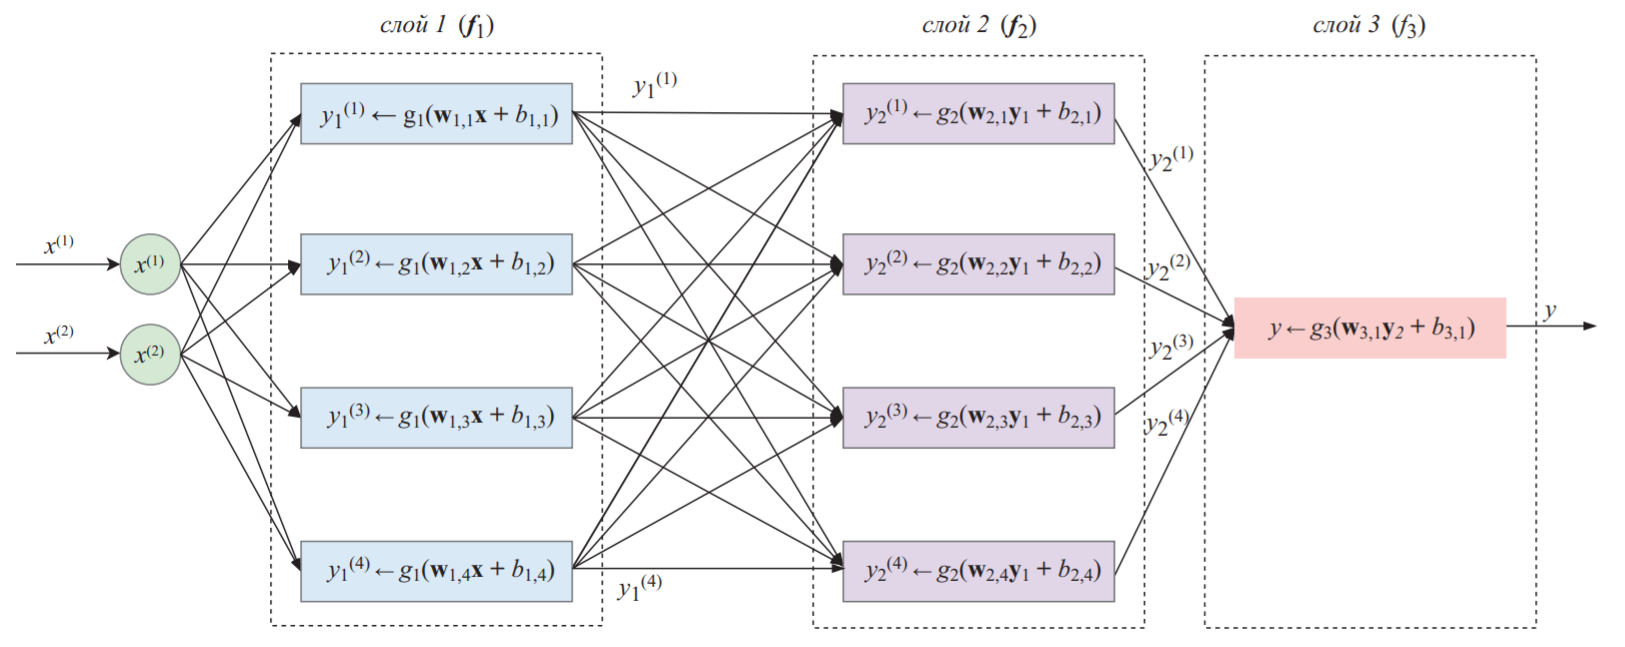
\includegraphics[scale=0.6]{figures/MLP.png}
	\caption{ Многослойный персептрон с двумерным входом, двумя слоями по четыре узла в каждом и выходным слоем с единственным узлом }\label{fig:MLP}
\end{figure}

Основная цель \emph{нелинейных} компонентов в функции $ f_{NN} $ состоит в том, чтобы позволить нейронной сети аппроксимировать \emph{нелинейные функции}. В отсутствие нелинейных компонентов $ f_{NN} $ была бы линейной, независимо от количества слоев. Причина в том, что $ \mathbf{W}_l z + \mathbf{b} $ является \underline{линейной} функцией, а линейная функция от линейной функции также является \underline{линейной}.

\section{Глубокое обучение}

Под глубоким обучением подразумевается обучение нейронных сетей, имеющих больше двух невыходных слоев. В прошлом обучение таких сетей усложнялось все больше с ростом количества слоев. В числе самых больших проблем назывались \emph{взрывной рост градиента} и \emph{затухание градиента}, поскольку для определения параметров сети использовался градиентный спуск.

Если проблема взрывного роста градиента решалась относительно просто, с применением таких простых методов, как \emph{ограничение градиента} и \emph{L1- или L2-регуляризация}, то проблема затухания градиента оставалась неразрешимой в течение десятилетий.

Для обновления значений параметров в нейронных сетях обычно используется алгоритм \emph{обратного распространения}. Обратное распространение -- это эффективный алгоритм вычисления \underline{градиентов} в нейронных сетях с использованием правила дифференцирования сложных функций.

\remark{
В каждой итерации обучения, в процессе градиентного спуска, параметры нейронной сети обновляются \underline{пропорционально} частной производной функции потерь для текущего параметра
}

Проблема в том, что иногда \emph{градиент} оказывается \emph{исчезающе малым}, что фактически мешает изменению значений некоторых параметров. В худшем случае это может \emph{полностью остановить обучение} нейронной сети.

Традиционные функции активации, такие функция гиперболического тангенса имеют градиенты в диапазоне $ (0, 1) $, при этом градиенты вычисляются на этапе обратного распространения по правилу дифференцирования сложных функций. В результате для вычисления градиентов предыдущих слоев (расположенных \emph{левее}) в $ n $-слойной сети производится перемножение $ n $ этих небольших чисел, из-за чего градиент экспоненциально уменьшается с увеличением $ n $. Это приводит к тому, что \emph{более ранние слои} обучаются намного \emph{медленее}, если вообще обучаются \cite[\strbook{96}]{burkov:2020}.

Однако современные реализации алгоритмов обучения нейронных сетей позволяют эффективно обучать очень глубокие нейронные сети (до нескольких сотен слоев). Это объясняется внедрением целого комплекса усовершенствований, включая ReLU, LSTM (и другие вентильные узлы), а также таких методов, как соединение с пропуском слоя, используемые в остаточных нейронных сетях, а также усовершенствованные версии алгоритма градиентного спуска.

\remark{
Когда в роли обучающих данных используются изображения, входные данные получаются слишком многомерными. Так как каждый пиксель в изображении -- это отдельный признак
}

\subsection{Сверточная нейронная сеть}

\emph{Сверточная нейронная сеть} (CNN) -- это особый вид сетей прямого распространения, который значительно сокращает количество параметров в глубокой нейронной сети с большим количеством узлов практически без потери качества модели.

Учитывая, что наиболее важная информация занимает на изображении ограниченную площадь, мы можем разделить изображение на квадратные фрагменты, используя метод скользящего окна. Затем обучить несколько \emph{небольших регрессионных моделей} одновременно, передавая каждой квадратный фрагмент.

Цель каждой небольшой регрессионной модели -- научиться обнаруживать определенный шаблон во фрагменте на вход. Например, одна небольшая модель может научиться определять небо, другая -- траву, третья -- края зданий и т.д.

Небольшие регрессионные модели в CNN напоминают модель многослойного персептрона, но имеют \emph{только по одному слою} \cite[\strbook{98}]{burkov:2020}. Чтобы обнаружить какой-либо шаблон, модель регрессии должна \emph{определить параметры матрицы} $ \mathbf{F}_{p \times p} $. Некотрый фрагмент может выглядеть как следующая матрица $ \mathbf{P} $
\begin{align*}
	\mathbf{P} =
	\begin{pmatrix}
		0 & 1 & 0 \\
		1 & 1 & 1 \\
		0 & 1 & 1
	\end{pmatrix}
\end{align*}

Этот фрагмент представляет шаблон с изображением креста. Небольшая регрессионная модель, которая будет обнаруживать такие шаблоны (и только их), должна обучить матрицу $ \mathbf{F} $ размером $ 3 \times 3 $, в которой параметры в позициях, соответствующих единицам во входном фрагменте, будут положительными цислами, а параметры в позициях, соотвествующих нулям, будут иметь значения, близкие к нулю. Если вычислить свертку матриц $ \mathbf{P} $ и $ \mathbf{F} $, полученное значение будет тем больше, чем больше $ \mathbf{F} $ похожа на $ \mathbf{P} $.

Оператор свертки определен только для матриц, имеющих одинаковое количество строк и столбцов (\pic{fig:conv}).

\begin{figure}[h]
	\centering
	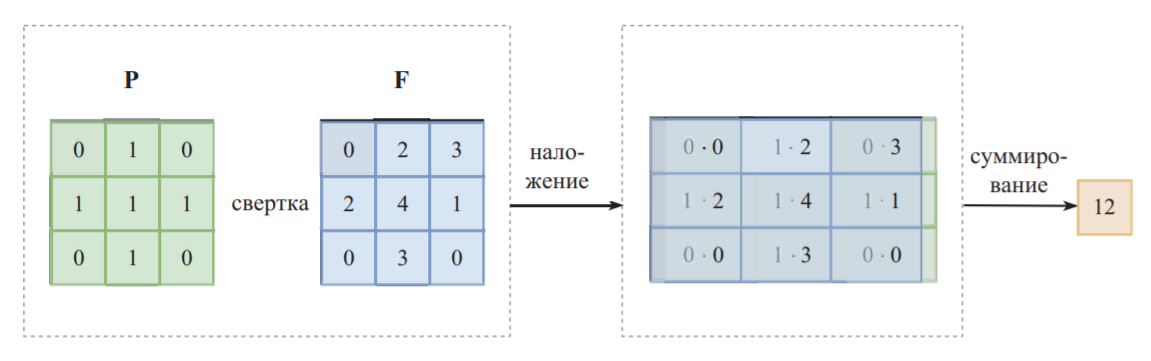
\includegraphics[scale=0.6]{figures/conv.png}
	\caption{ Свертка двух матриц }\label{fig:conv}
\end{figure}

Например, если подать на вход фрагмент $ \mathbf{P} $, имеющий L-шаблон
\begin{align*}
	\mathbf{P} = 
	\begin{pmatrix}
		1 & 0 & 0 \\
		1 & 0 & 0 \\
		1 & 1 & 1
	\end{pmatrix},
\end{align*}
тогда свертка с $ \mathbf{F} $ даст в результате меньшее значение: 5.

\remark{
То есть чем больше фрагмент похож на фильтр, тем выше значение операции свертки
}

Каждый фильтр в первом (самом левом) слое скользит -- свертывает -- по входному изображению слева направо, сверху вниз, и в каждой итерации вычисляет значение свертки.

\underline{Матрица фильтра} (по одной для каждого фильтра в каждом слое) и \underline{значения смещения} являются \emph{обучаемыми параметрами}, которые оптимизируются с испльзованием градиентного спуска с обратным распространением.

Нелинейность применяется к сумме свертки и смещения, т.е. $ \sigma (\mathbf{P} \circ \mathbf{F} + b) $. Как правило, во всех скрытых слоях используется функция активации ReLU. Функция активации в выходном слое зависит от решаемой задачи. Функция активации в выходном слое зависит от решаемой задачи.

Если CNN имеет один сверточный слой, следующий за другим сверточным слоем, то последующий слой $ l + 1 $ будет обрабатывать выходные данные предыдущего слоя $ l $, как коллекцию $ size_l $ матриц изображения. Такая коллекция называется \emph{томом}. Размер колллекции называется \emph{глубиной тома}. Каждый фильтр в слое $ l + 1 $ выполняет свертку \underline{всего тома}. Свертка фрагмента тома -- это просто сумма сверток соответствующих фрагментов отдельных матриц, из которых состоит том.

\begin{figure}[h]
	\centering
	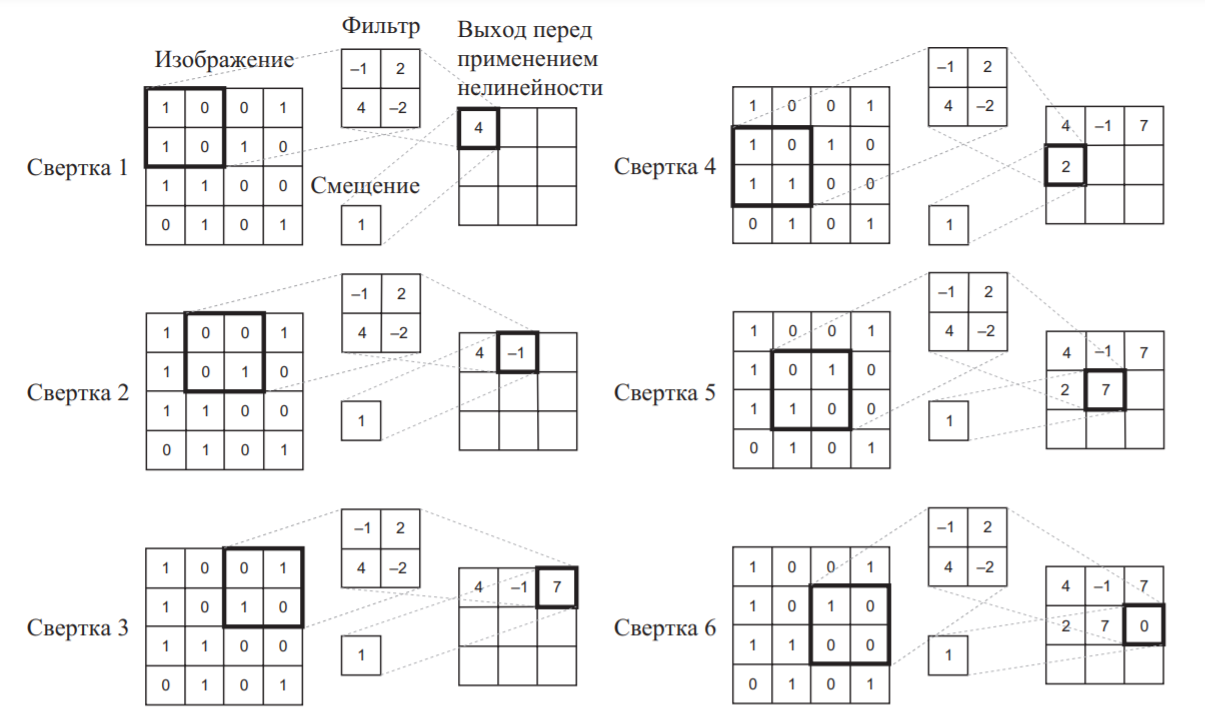
\includegraphics[scale=0.7]{figures/conv-3.png}
	\caption{ Фильтр, свертывающий изображение }\label{fig:conv-3}
\end{figure}

Свертки имеют два важных свойства -- шаг и дополнение. Шаг -- это величина одного шага смещения окна. Дополнение позволяет получить увеличенную выходную матрицу. Это ширина рамки с дополнительными ячейками, которые добавляются вокруг изображения (или тома) перед сверткой с помощью фильтра. Обычно дополнительные ячейки, формирующие дополнение, содержат нули.

Дополнение может пригодиться при использовании более крупных фильтров, позволяя им лучше <<сканировать>> границы изображения.

Подобно свертке операция подвыборки (пулинга, субдискретизации) имеет гиперпараметры -- размер фильтра и шаг. Как правило, слой подвыборки следует за сверточным слоем и получает на входе выходные данные свертки. Когда подвыборка применяется к тому, каждая матрица в этом томе обрабатывается независимо от других. То есть в результате применения подвыборки к тому получается том с той же глубиной.

\remark{
	Подвыборка (пулинг, субдискретизация) имеет только гиперпараметры и не имеет обучаемых параметров
}

На практике обычно используются фильтры с размером 2 или 3 и с шагом 2. Подвыборка с определением максимального значения более популярна, чем с определением среднего, и часто дает лучшие результаты.

\subsection{Рекуррентная нейронная сеть}

Рекурентные нейронные сети (RNN) используется для маркировки, классификации или генерации последовательностей. Последовательность -- это матрица, каждая строка которой является вектором признаков и в которой порядок строк имеет значение. 

Реккурентная нейронная сеть не является сетью прямого распространения: \underline{она содержит циклы}. Идея состоит в том, что каждый узел $ u $ реккурентного слоя $ l $ имеет \emph{вещественное состояние} $ h_{l,u} $. Состояние можно рассматривать как \emph{память узла}. В RNN каджый узел $ u $ в каждом слое $ l $ имеет два входа: вектор состояний из предыдущего слоя $ l - 1 $ и вектор состояний из этого же слоя $ l $, но из \emph{предыдущего временного шага}.

Для иллюстрации рассмотрим первый и второй рекуррентные слои в сети RNN. Первый (самый левый) слой получает на входе вектор признаков. Второй слой получает на входе выходные данные из первого слоя (\pic{fig:rnn}).

Каждый обучающий образец представлен матрицей, в которой каждая строка является вектором признаков. 

\begin{figure}[h]
	\centering
	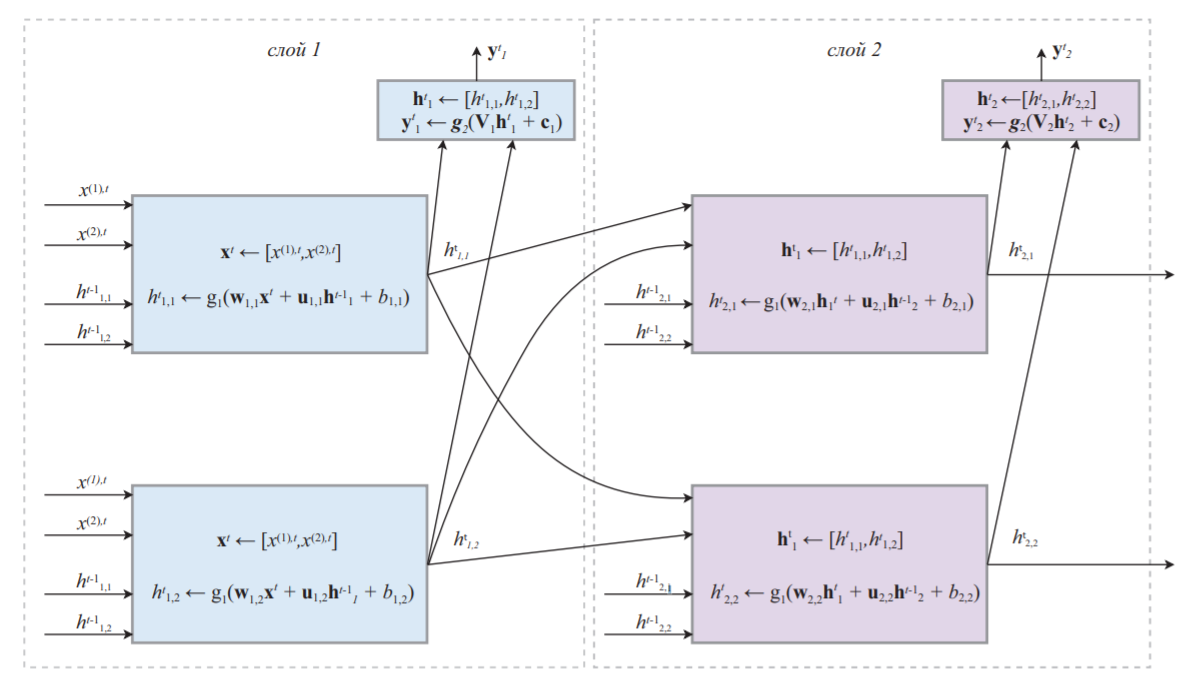
\includegraphics[scale=0.75]{figures/rnn.png}
	\caption{ Первые два слоя в рекуррентной нейронной сети. На вход подается двумерный вектор признаков. Каждый слой имеет два узла }\label{fig:rnn}
\end{figure}

Для обучения моделей RNN используется специальная версия обратного распространения, называемая \emph{обратным распространением во времени}.

Обе функции -- $ \tanh $ и softmax -- страдают проблемой затухания градиентов. Даже если сеть RNN имеет только один или два рекуррентных слоя, из-за последовательного характера входных данных обратное распространение <<развертывает>> сеть с течением времени. С точки зрения вычисления градиента это означает, что чем длиннее входная последовательность, тем глубже полчается развернутая сеть.

Другая проблема, характерая для RNN, заключается в обработке долгосрочных зависимостей. По мере увеличения длины входной последовательности векторы признаков, находящиеся в начале последовательности, постепенно <<забываются>>, потому что состояние всех узлов, которые играют роль памяти сети, в значительной степени зависит от векторов признаков, прочитанных последними.

Наиболее эффективными рекуррентными моделями нейронных сетей, используемые на практике, являются вентильные RNN. К ним относятся сети с \emph{долгой краткосрочной памятью} (LSTM) и сети с вентильными рекуррентными узлами (GRU).

В рекуррентных нейронных сетях операции чтения, записи и стирания информации, хранящейся в каждом узле, контролируются функциями активации, которые принимают значения в диапазоне $ (0, 1) $. Обученная нейронная сеть может <<прочитать>> входную последовательность векторов признаков и на некотором раннем временном шаге $ t $ решить сохранить конкретную информацию о векторах признаков. Эта информация о более ранних векторах признаков может позже использоваться моделью для обработки векторов признаков в конце входной последовательности.

Решение о том, какую информацию хранить и когда разрешать чтение, запись и удаление, принимают узлы. Эти решения принимаются на основе данных и реализуются через идею вентилей. Есть несколько архитектур управляемых узлов. Простая, но эффективная называется \emph{минимальным вентильным узлом} и состоит из \emph{ячейки памяти} и \emph{вентиля забывания}
\begin{align*}
	\tilde{h}^t_{l,u} \leftarrow \tanh (\mathbf{w}_{l,u} \mathbf{x}^t + \mathbf{u}_{l,u} \mathbf{h}_l^{t-1} + b_{l,u}),\\
	\Gamma_{l,u}^t \leftarrow \sigma (\mathbf{m}_{l,u} \mathbf{x}^t + \mathbf{o}_{l,u} \mathbf{h}^{t - 1} + a_{l, u}),\\
	h^t_{l,u} \leftarrow \Gamma^t_{l,u} \tilde{h}_l^t + \big( 1 - \Gamma^t_{l,u}  \big) h_l^{t - 1},\\
	\mathbf{h}_l^t \leftarrow \big[ h_{l,1}^t, \ldots, h_{l, size_l}^t \big],\\
	\mathbf{y}_l^t \leftarrow \mathbf{g}(\mathbf{V}_l \mathbf{h}_l^t + \mathbf{c}_{l,u}),
\end{align*}
где $ \mathbf{g} $ -- функция softmax.

Если вентиль $ \Gamma_{l,u}^t $ близок к 0, тогда ячейка памяти сохраняет значение, полученное на предыдущем временном шаге $ h_l^{t-1} $. Если вентиль $ \Gamma_{l,u}^t $ близок к 1, значение ячейки памяти затирается новым значением $ \tilde{h}^t_{l,u} $.


\section{Приемы работы с библиотекой plotly}

Шаблонный код для JupyterLab
\begin{lstlisting}[
style = ironpython,
numbers = none
]
# ячейка
import numpy as np
import plotly.graph_objs as go
from plotly.offline import (
	download_plotlyjs,
	init_notebook_mode,
	plot,
	iplot,
)
# ячейка
init_notebook_mode(connected=True)
# ячейка
fig = go.Figure()
# ячейка
fig.add_traces([
	go.Scatter(y=np.random.randn(100).cumsum(), name="curve-1"),
	go.Scatter(y=np.random.randn(100).cumsum(), name="curve-2"),
]);
# ячейка
fig.update_layout(
	title=dict(
		text=(
			"<i>Реализации значений переменных</i>"),       
		font=dict(
			family="Arial",
			size=18,
			color="#07689F",
		),
	),
	xaxis_title="<i>Имена переменных</i>",
	yaxis_title="<i>Значение переменной</i>",
	xaxis=dict(
		showline=True,
		showgrid=False,
		showticklabels=True,
		linecolor="rgb(204, 204, 204)",
		linewidth=1.5,
		ticks="outside",
		tickfont=dict(
			family="Arial",
			size=15,
			color="rgb(82, 82, 82)",
		),
	),
	yaxis=dict(
		showgrid=False,
		zeroline=False,
		showline=True,
		showticklabels=True,
		linecolor="rgb(204, 204, 204)",
		linewidth=1.5,
		ticks="outside",
		tickfont=dict(
			family="Arial",
			size=15,
			color="rgb(82, 82, 82)",
		),
	),
	autosize=False,
	margin=dict(
		autoexpand=False,
		l=70,
		r=10,
		t=50,
	),
	showlegend=True,
	plot_bgcolor="white",
	legend_title_text="<i>Имя блока легенды</i>",
	legend=dict(
		orientation="v",
		yanchor="bottom",
		y=0.01,
		xanchor="right",
		x=0.99,
		font=dict(family="Arial", size=12, color="black"),
	),
	font=dict(
		family="Arial",
		size=13,
	),
)
\end{lstlisting}

Если теперь воспользоваться функцией \texttt{plot}, то в текущей директории проекта будет создан \texttt{html}-файл интерактивного графика, который автоматически откроется в браузере
\begin{lstlisting}[
style = ironpython,
numbers = none
]
plot(fig, filename="test-sample.html")
\end{lstlisting}


\section{Приемы работы с библиотекой анализа временных рядов ETNA}

\subsection{Перекрестная проверка на временных рядах}

Перекрестную проверку с расширяющимся окном (или на скользящем окне) в бибилотеке ETNA можно выполнить с помощью метода \verb|.backtest()|. Этот метод возвращает три кадра данных: кадр данных с метриками по каждой тестовой выборке перекрестной проверки, кадр данных с прогнозами и кадр данных с временными метками обучающего и тестового поднаборов данных.

В перекрестной проверке расширяющися окном количество наблюдений, использованных для обучения в каждой итерации, растет с числом итераций, предоставляет все больший объем данных для обучения.

\begin{figure}[h]
	\centering
	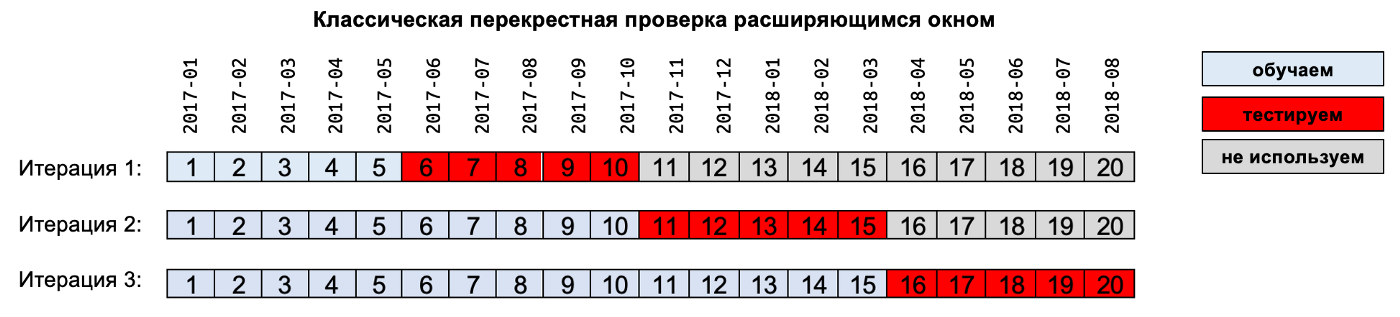
\includegraphics[scale=0.3]{figures/cross_val_ts.png}
	\caption{ Перекрестная проверка на временном ряду \emph{расширяющимся} окном }\label{fig:cross_val_ts}
\end{figure}

Для тестирования мы каждый раз берем совершенно новые более поздние наблюдения. Обучающая выборка прирастает на количество наблюдений, равное горизонту прогнозирования.

При необходимости обучение модели в каждом разбиении можно сделать последовательным, используя в каждой итерации для обучения фиксированное количество наиболее свежих (поздних) наблюдений, предшествующих точке разбиения. Таким образом, в каждой новой итерации мы будем обучаться на более свежих данных, обучающая выборка каждый раз сдвигается вперед по временной оси (обычно на горизонт прогнозирования) и такой способ проверки называют перекрестной проверкой скользящим окном (sliding/rolling window).

\begin{figure}[h]
	\centering
	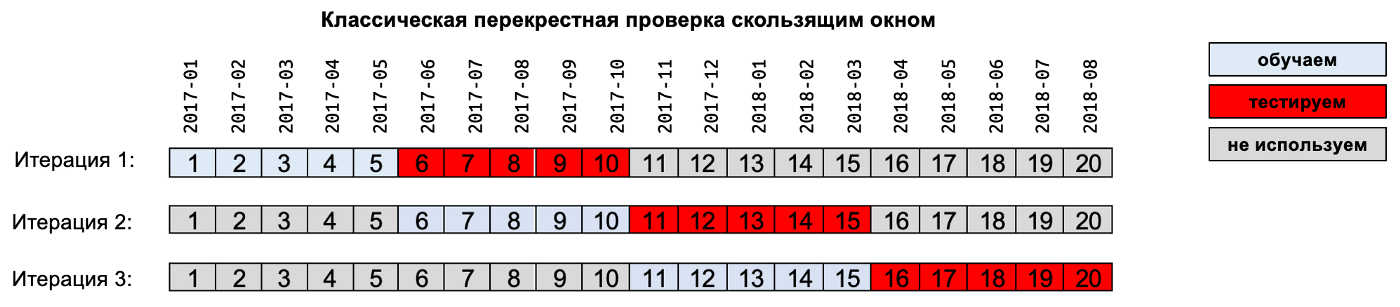
\includegraphics[scale=0.3]{figures/cross_val_rol_ts.png}
	\caption{ Перекрестная проверка \emph{на скользящем} окне }\label{fig:cross_val_rol_ts}
\end{figure}

С каждой итерацией обучающая выборка использует все более свежие наблюдения, при этом для тестирования мы каждый раз берем совершенно новые более поздние наблюдения. Размер обучающей выборки остается неизменным, поэтому в ETNA этот вид проверки назван \verb|constant|.

NB При выполнении перекрестной проверки для временных рядов полезно помнить ряд правил:
\begin{itemize}
	\item Размер тестовой выборки, как правило, определяется горизонтом прогнозирования, а тот в свою очередь определяется бизнес-требования. Если вы предсказываете на 14 дней вперед, то и тестовая выборка должна включать 14 более поздних наблюдений.
	
	\item Размер тестовой выборки остается постоянным. Это значит, что метрики качества, полученные в результате вычислений прогнозов каждой обученной модели по тестовому набору, будут последовательны и их можно объединять и сравнивать.
	
	\item Размер обучающей выборки не может быть меньше тестовой выборки.
	
	\item Если данные содержат сезонность, обучающая выборка должна содержать не менее двух полных сезонных циклов (правило $ 2L $, где $ L $ -- количество периодов в полном сезонном цикле, необходимое для инициализации параметров некоторых моделей, например, для вычисления исходного значения тренда в модели тройного экспонециального сглаживания), учитывая уменьшение длины ряда при выполнении процедур обычного и сезонного дифференциирования.
	
	\item Если применяются переменные -- лаги, разности на лагах, скользящие статистики, то каждый раз для получения значений в тестовой выборке используются только данных обучающей выборки.
\end{itemize}

Перекрестную проверку расширяющимся окном можно модифицировать так, чтобы обучающая выборка прирастала на количество наблюдений меньше горизонта прогнозирования и тогда в тестовую выборку попадут наблюдения, уже попадавшие в тестовую выборку на предыдущей итерации. Это позволяет управлять скоростью обновления модели, лучше выявлять аномальные, нетипичные наблюдения, которые плохо предсказываются, точнее определить момент ухудшения качества модели.

\begin{figure}[h]
	\centering
	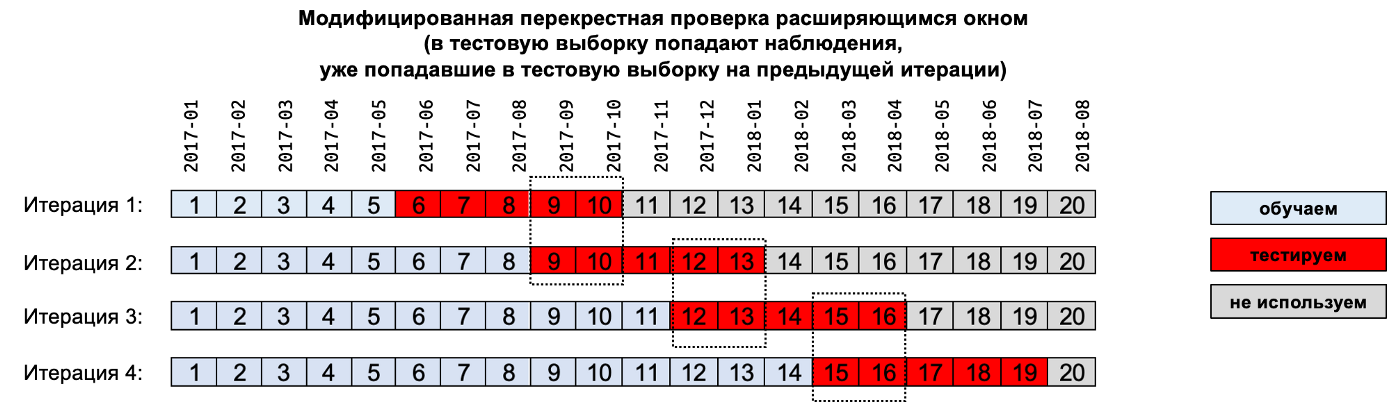
\includegraphics[scale=0.3]{figures/cross_val_expand_ts.png}
	\caption{ Модфицированная перекрестная проверка расширяющимся окном }\label{fig:cross_val_expand_ts}
\end{figure}

Перекрестную проверку скользящим окном тоже можно модифицировать так, чтобы обучающая выборка сдвигалась вперед не на весь горизонт прогнозирония, а на половину или на треть, и тогда в тестовую выборку попадут наблюдения, уже попадавшие в тестовую выборку на предыдущей итерации. Это позволяет управлять скоростью обновления модели, лучше выявлять аномальные, нетипичные наблюдения, которые плохо предсказываются, точнее определять момент ухудшения качества модели.

\begin{figure}[h]
	\centering
	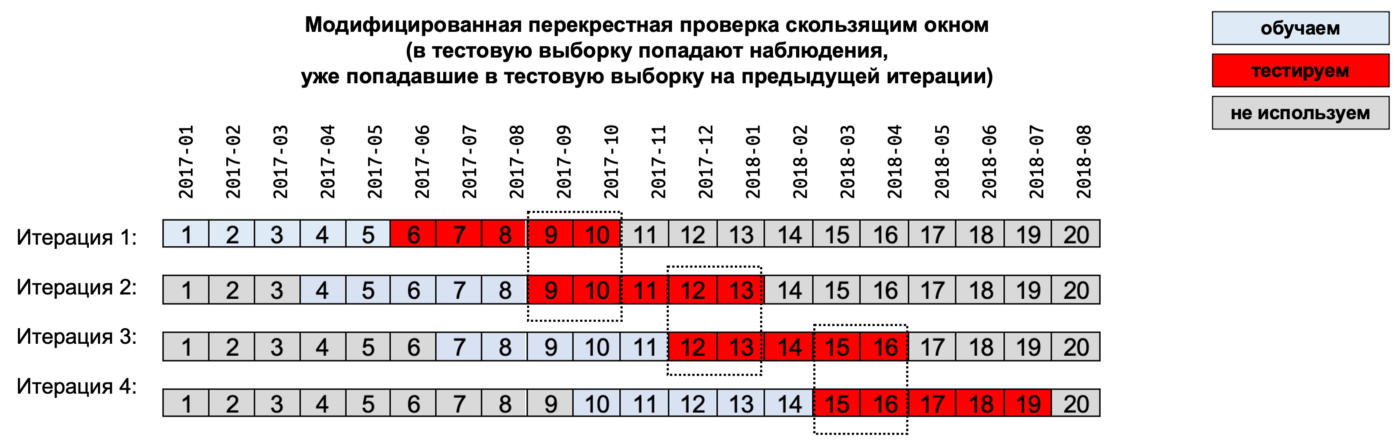
\includegraphics[scale=0.3]{figures/cross_val_rol_modif_ts.png}
	\caption{ Модфицированная перекрестная проверка скользящим окном }\label{fig:cross_val_rol_modif_ts}
\end{figure}

Однако, в библиотеке ETNA и библиотеке scikit-learn с помощью класса TimeSeriesSplit нельзя корректно реализовать вышеописанные модификации.

При использовании перекрестной проверки расширяющимся окном модель в большей степени нацелена на обнаружение глобальных паттернов и менее склонна к изменениям, т.е. более консервативна. При использовании перекрестной проверки скользящим окном используется меньше данных, модель быстрее меняет поведение, т.е. менее консервативна. В ситуации, когда вы уверены, что процесс, генерирующий данные, изменился или неоднократно менялся в течение периода, охватывающего исторические данные, используйте перекрестную проверку скользящим окном.

Для рынков товаров с низкой вовлеченностью (товаров повседневного спроса), в ситуации, когда вы уверены или у вас есть доказательства, что процесс, генерирующий данные, остается неизменным или претерпевает несущественные изменения, перекрестная проверка расширяющимся окном может быть более полезна.

\remark{
Важно помнить, что во временных рядах \emph{перекрестная проверка}, которую вы применяете, является \emph{прообразом} вашей \emph{производственной системы}. Если вы применяли для валидации перекрестную проверку расширяющимся окном, то и в производстве вы должны обучать модель на обучающей выборке возрастающего объема и обновлять в том же темпе, что обновляли в ходе перекрестной проверки (на весь горизонт прогнозирования, на половину горизонта и т.д.)
}

Наконец, поскольку в рамках перекрестной проверки расширяющимся окном мы на каждой итерации обучаем модель на выборке все большего объема, при использовании моделей на основе градиентного бустинга это может потребовать коррекции темпа обучения, количества деревьев и максимальной глубины. 

\subsection{CatBoost. Базовая модель с конструированием признаков}

В ETNA есть два класса-обертки над классом \texttt{CatboostRegressor}: \texttt{CatBoostModePerSegment} и \texttt{CatBoostModelMultiSegment}. Разница заключается в том, что класс \texttt{CatBoostModelPerSegment} обучает отдельную модель для каждого сегмента, а класс \texttt{CatBoostModelMultiSegment} -- одну модель для всех сегментов.

Для создания признаков можно использовать классы-трансформеры:
\begin{itemize}
	\item \texttt{LagTransform} для генерации лагов,
	
	\item \texttt{MeanTransform} для вычисления скользящего среднего по заданному окну.
\end{itemize}

\remark{
Ширину окна $ w $ для скользящих статистик \emph{рекомендуется} задавать равной или превышающей горизонт прогнозирования $ h $, т.е. $ w \geqslant h $. То же относится и к лагам. Порядок лага $ lag $ должен быть равен или превышать горизонт прогнозирования, т.е. $ lag \geqslant h $. В противном случае признаки тествого поднабора данных (построенные на лагах с  порядком меньшим горизонта прогнозирования), будут использовать значения целевой переменной из тестового поднабора данных (утечка)
}

С помощью параметра \verb|in_column| класса-трансформера задаем переменную, которую нужно преобразовать или на основе которой нужно создать признаки (по умолчанию этой переменной будет переменная \texttt{target}). С помощью параметра \verb|out_column| (этот параметр есть у всех классов-трансформеров, создающих признаки) можно задать имена генерируемых переменных.

Для более надежной оценки качества модели следует восопользоваться \emph{перекрестной проверкой расширяющимся окном} с помощью класса \texttt{Pipeline}.

Создадим список преобразований. В данном случае он включать формирование лагов и скользящего среднего на каждой итерации перекрестной проверки.

\begin{lstlisting}[
style = ironpython,
numbers = none
]
lags = LagTransform(in_column="target", lags=list(range(8, 24, 1)), out_column="lag")
mean8 = MeanTransform(in_column="target", window=8, out_column="mean8")
transforms = [lags, mean8]
\end{lstlisting}

Теперь создаем конвейер для выполнения перекрестной проверки расширяющимся окном, передав в него модель, список процедур формирования признаков (лагов и скользящего среднего) и горизонт прогнозирования
\begin{lstlisting}[
style = ironpython,
numbers = none
]
model = CatBoostModelMultiSegment()
model.fit(train_ts)

pipeline = Pipeline(
    model=model,
    transforms=transforms,
    horizon=HORIZON,
)
# перекрестная проверка расширяющимся окном
metrics_df, _, _ = pipeline.backtest(
    ts=ts,
    mode="expand",
    metrics=[smape],
)
\end{lstlisting}

Класс \texttt{Pipeline} можно использовать для перекрестной проверки сразу нескольких моделей
\begin{lstlisting}[
style = ironpython,
numbers = none
]
# задаем конвейер преобразований для модели наивного прогноза
naive_pipeline = Pipeline(
    model=NaiveModel(lag=12), transforms=[], horizon=HORIZON)
# задаем конвейер преобразований для Prophet
prophet_pipeline = Pipeline(
    model=ProphetModel(), transforms=[], horizon=HORIZON
)
# задаем конвейер преобразований для CatBoost
catboost_pipeline = Pipeline(
    model=CatBoostModelMultiSegment(),
    transforms=[LagTransform(lags=[8, 9, 10, 11, 12], 
    in_column='target')],
    horizon=HORIZON
)
# задаем список имен конвейеров
pipeline_names = ['naive', 'prophet', 'catboost']
# задаем список конвейеров
pipelines = [naive_pipeline, prophet_pipeline, catboost_pipeline]
# задаем пустой список метрик
metrics = []
# записываем метрики в список
for pipeline in pipelines:
    metrics.append(
        pipeline.backtest(
        ts=ts, metrics=[MAE(), MSE(), SMAPE(), MAPE()], 
        n_folds=3, aggregate_metrics=True
    )[0].iloc[:, 1:]
)

# конкатенируем метрики
metrics = pd.concat(metrics)
# в качестве индекса используем список имен конвейеров
metrics.index = pipeline_names
\end{lstlisting}

С помощью класса \texttt{VotingEnsemble} можно выполнить обучение и перекрестную проверку \emph{ансамбля моделей}. Веса моделей можно задавать с помощью параметра \texttt{weights}
\begin{lstlisting}[
style = ironpython,
numbers = none
]
# создаем экземпляр класса VotingEnsemble
voting_ensemble = VotingEnsemble(pipelines=pipelines, 
weights=[1, 2, 4], 
n_jobs=4)
# получаем метрики
voting_ensamble_metrics = voting_ensemble.backtest(
    ts=ts,
    metrics=[MAE(), MSE(), SMAPE(), MAPE()], 
    n_folds=3,
    aggregate_metrics=True,
    n_jobs=2
)[0].iloc[:, 1:]
voting_ensamble_metrics.index = ['voting ensemble']
\end{lstlisting}

С помощью класса \texttt{StackingEnsemble} можно выполнить \emph{стекинг}. Мы прогнозируем будущее, используя метамодель (линейную регрессию по умолчанию) для объединения прогнозов моделей в списке конвейеров. С помощью параметров \verb|final_model| можно задать метамодель. С помощью \verb|features_to_use| можно задавать признаки для метамодели
\begin{itemize}
	\item \texttt{None}: метамодель в качестве признаков может использовать прогнозы моделей конвейеров,
	
	\item \texttt{List}: прогнозы моделей конвейеров плюс признаки из списка (в виде строковых значений),
	
	\item \texttt{"all"}: все доступные признаки.
\end{itemize}

С помощью параметра \texttt{cv} задаем количество тестовых выборок перекрестной выборки (используем не для оценки моделей, а для получения прогнозов, которые станут у нас потом признаками).

Под капотом происходит примерно следующее. Допустим, запустили перекрестную проверку расширяющимся окном, получили 5 тестовых выборок, прогнозы каждой из модели конвейера в 5 тестовых выбоках стали признаками. Затем снова запускаем проверку расширяющимся окном, по этим признакам строим метамодель -- линейную регрессию, берем прогнозы в 3 тестовых выборках и усредняем
\begin{lstlisting}[
style = ironpython,
numbers = none
]
# создаем экземпляр класса StackingEnsemble,
# признаки - прогнозы конвейеров
stacking_ensemble_unfeatured = StackingEnsemble(
    features_to_use='None', pipelines=pipelines, 
    n_folds=10, n_jobs=4)
# выполняем стекинг
stacking_ensamble_metrics = stacking_ensemble_unfeatured.backtest(
    ts=ts, metrics=[MAE(), MSE(), SMAPE(), MAPE()], n_folds=3, 
    aggregate_metrics=True, n_jobs=2)[0].iloc[:, 1:]
stacking_ensamble_metrics.index = ['stacking ensemble']
stacking_ensamble_metrics
\end{lstlisting}

\subsection{Пользовательские классы для вычисления скользящих статистик}

Можно писать свои собственные классы для вычисления скользящих статистик и обучения моделей. Допустим, мы хотим использовать не только скользящие средние, но и скользящие средние абсолютные отклонения
\begin{lstlisting}[
style = ironpython,
numbers = none
]
# пишем класс MadTransform, вычисляющий скользящие
# средние абсолютные отклонения
class MadTransform(WindowStatisticsTransform):
    """
    MadTransform вычисляет среднее абсолютное отклонение
    (mean absolute deviation - mad) для заданного окна.
    """
		def __init__(
			self,
			in_column: str,
			window: int,
			seasonality: int = 1,
			min_periods: int = 1,
			fillna: float = 0,
			out_column: Optional[str] = None
		):
		"""
		Параметры
		----------
		in_column: str
		имя обрабатываемого столбца
		window: int
		ширина окна для агрегирования
		out_column: str, optional
		имя результирующего столбца. Если не задано, 
		используем __repr__()
		seasonality: int
		коэффициент сезонности
		min_periods: int
		Минимальное количество наблюдений в окне 
		для агрегирования
		fillna: float
		значение для заполнения значений NaN
		"""
		self.in_column = in_column
		self.window = window
		self.seasonality = seasonality
		self.min_periods = min_periods
		self.fillna = fillna
		self.out_column = out_column
		super().__init__(
		window=window,
		in_column=in_column,
		seasonality=seasonality,
		min_periods=min_periods,
		out_column=self.out_column 
		if self.out_column is not None 
		else self.__repr__(),
		fillna=fillna,
	)
	def _aggregate_window(
		self, series: pd.Series
	) -> float:
		"""Вычисляет mad для серии."""
		tmp_series = self._get_required_lags(series)
		return tmp_series.mad(**self.kwargs)
\end{lstlisting}

Теперь предположим, мы хотим использовать LightGBM вместо CatBoost. Нам понадобиться класс LGBRegressor и базовые классы библиотеки ETNA \texttt{Model} и \texttt{PerSegmentModel}.

Сначала надо написать ядро -- внутренний класс \verb|_LBGMModel|, в котором используется \texttt{LGBMRegressor}. Символ нижнего подчеркивания указывает, что данный класс будет использоваться внутри других классов. У класса \verb|_LGBModel| будут два метода \texttt{fit()} и \texttt{predict()}.

\begin{lstlisting}[
style = ironpython,
numbers = none
]
# пишем ядро - внутренний класс _LGBMModel,
# внутри - класс LGBMRegressor
class _LGBMModel:
	def __init__(
		self,
		boosting_type='gbdt',
		num_leaves=31,
		max_depth=-1,
		learning_rate=0.1,
		n_estimators=100,
		**kwargs
	):
		self.model=LGBMRegressor(
			boosting_type=boosting_type,
			num_leaves=num_leaves,
			max_depth=max_depth,
			learning_rate=learning_rate,
			n_estimators=n_estimators,
			**kwargs
		)
	def fit(self, df: pd.DataFrame):
		features = df.drop(columns=['timestamp', 'target'])
		target = df['target']
		self.model.fit(X=features, y=target)
		return self
		
	def predict(self, df: pd.DataFrame):
		features = df.drop(columns=['timestamp', 'target'])
		pred = self.model.predict(features)
		return pred
\end{lstlisting}

Вспомним, что мы можем строить отдельную модель для каждого сегмента и одну модель для всего набора (т.е. всех сегментов). Значит мы можем написать два класса. Начнем с класса, который будет строить отдельную модель для каждого сегмента. Назовем его \texttt{LGBModelPerSegment}. Для этого воспользуемся наследованием, нам понадобится базовый класс \texttt{PerSegmentModel}

\begin{lstlisting}[
style = ironpython,
numbers = none
]
# пишем класс LGBMModelPerSegment, который строит 
# отдельную модель LGBM для каждого сегмента
class LGBMModelPerSegment(PerSegmentModel):
	def __init__(
		self,
		boosting_type='gbdt',
		num_leaves=31,
		max_depth=-1,
		learning_rate=0.1,
		n_estimators=100,
		**kwargs
	):
		self.kwargs = kwargs
		model = _LGBMModel(
			boosting_type=boosting_type,
			num_leaves=num_leaves,
			max_depth=max_depth,
			learning_rate=learning_rate,
			n_estimators=n_estimators,
			**kwargs
		)
		super(LGBMModelPerSegment, self).__init__(
			base_model=model)
\end{lstlisting}

Теперь напишем класс, который будет строить одну модель для всех сегментов. Назовем его \texttt{LGBModelMultiSegment}. Для этого вновь воспользуемся наследованием, нам понадобится базовый класс \texttt{Model}

\begin{lstlisting}[
style = ironpython,
numbers = none
]
# пишем класс LGBMModelMultiSegment, который строит 
# одну модель LGBM для всех сегментов
class LGBMModelMultiSegment(Model):
	def __init__(
		self,
		boosting_type='gbdt',
		num_leaves=31,
		max_depth=-1,
		learning_rate=0.1,
		n_estimators=100,
		**kwargs
	):
		self.kwargs = kwargs
		super(LGBMModelMultiSegment, self).__init__()
		self._base_model=_LGBMModel(
			boosting_type=boosting_type,
			num_leaves=num_leaves,
			max_depth=max_depth,
			learning_rate=learning_rate,
			n_estimators=n_estimators,
			**kwargs
		)
		
	def fit(self, ts: TSDataset):
		# превращаем TSDataset в датафрейм pandas
		# с плоским индексом
		df = ts.to_pandas(flatten=True)
		df = df.dropna()
		df = df.drop(columns='segment')
		self._base_model.fit(df=df)
		return self
		
	def forecast(self, ts: TSDataset):
		result_list = list()
		# собираем новый датафрейм с помощью self._forecast_segment
		# из базового класса
		for segment in ts.segments:
			segment_predict = self._forecast_segment(
				self._base_model, segment, ts)
			result_list.append(segment_predict)
			
		result_df = pd.concat(result_list, ignore_index=True)
		result_df = result_df.set_index(['timestamp', 'segment'])
		
		df = ts.to_pandas(flatten=True)
		df = df.set_index(['timestamp', 'segment'])
		# заменяем пропуски прогнозами
		df = df.combine_first(result_df).reset_index()
		df = TSDataset.to_dataset(df)
		ts.df = df
		# выполняем обратные преобразования
		ts.inverse_transform()
		
		return ts
\end{lstlisting}

Аналогично можно реализовать XGBoost в ETNA. Пишем класс \verb|_XGBModel|
\begin{lstlisting}[
style = ironpython,
numbers = none
]
class _XGBModel:
    def __init__(
        self,
        booster="gbtree",
        max_depth=3,
        learning_rate=0.1,
        n_estimators=100,
        **kwargs,
    ):
        self.model=XGBRegressor(
            booster=booster,
            max_depth=max_depth,
            learning_rate=learning_rate,
            n_estimators=n_estimators,
            **kwargs,
        )
        
    def fit(
        self,
        df: pd.DataFrame,
    ):
        features = df.drop(columns=["timestamp", "target"])
        for col in features.columns.tolist():
            features[col] = features[col].astype("category").cat.codes
        target = df["target"]
        self.model.fit(X=features, y=target)
        return self
        
    def predict(
        self,
        df: pd.DataFrame,
    ):
        features = df.drop(columns=["timestamp", "target"])
        for col in features.columns.tolist():
            features[col] = features[col].astype("category").cat.codes
        pred = self.model.predict(features)
        return pred
\end{lstlisting}

Пишем классы \texttt{XGBModePerSegment} и \texttt{XGBModelMultiSegment}
\begin{lstlisting}[
style = ironpython,
numbers = none
]
# пишем класс XGBModelPerSegment, который строит 
# отдельную модель XGB для каждого сегмента
class XGBModelPerSegment(PerSegmentModel):
	def __init__(
		self,
		booster='gbtree',
		max_depth=3,
		learning_rate=0.1,
		n_estimators=200,
		**kwargs
	):
	self.kwargs = kwargs
	model = _XGBModel(
		booster=booster,
		max_depth=max_depth,
		learning_rate=learning_rate,
		n_estimators=n_estimators,
		**kwargs
	)
	super(XGBModelPerSegment, self).__init__(
		base_model=model)
		
# пишем класс XGBModelMultiSegment, который строит 
# одну модель XGB для всех сегментов
class XGBModelMultiSegment(Model):
	def __init__(
		self,        
		booster='gbtree',
		max_depth=3,
		learning_rate=0.1,
		n_estimators=100,
		**kwargs
	):
		self.kwargs = kwargs
		super(XGBModelMultiSegment, self).__init__()
		self._base_model=_XGBModel(
			booster=booster,
			max_depth=max_depth,
			learning_rate=learning_rate,
			n_estimators=n_estimators,
			**kwargs
	)
	
	def fit(self, ts: TSDataset):
		# превращаем TSDataset в датафрейм pandas
		# с плоским индексом
		df = ts.to_pandas(flatten=True)
		df = df.dropna()
		df = df.drop(columns='segment')
		self._base_model.fit(df=df)
		return self
		
	def forecast(self, ts: TSDataset):
		result_list = list()
		# собираем новый датафрейм с помощью 
		# self._forecast_segment 
		# из базового класса
		for segment in ts.segments:
			segment_predict = self._forecast_segment(
				self._base_model, segment, ts)
			result_list.append(segment_predict)
			
		result_df = pd.concat(result_list, ignore_index=True)
		result_df = result_df.set_index(['timestamp', 'segment'])
		
		df = ts.to_pandas(flatten=True)
		df = df.set_index(['timestamp', 'segment'])
		# заменяем пропуски прогнозами
		df = df.combine_first(result_df).reset_index()
		df = TSDataset.to_dataset(df)
		ts.df = df
		# выполняем обратные преобразования
		ts.inverse_transform()

		return ts
\end{lstlisting}

\remark{
Порядок лагов не должен быть меньше длины горизонта! Потому как в противном случае, признаки тествого поднабора данных, построенные на лагах, будут использовать информацию из целевой переменной тестового поднабора данных (утечка!)
}

Таким образом, необходимо создаватвь лаговые переменные так, чтобы они не проникали в тестовый набор. Лаги вида $ L_{t-k} $ лучше создавать так, чтобы $ k $ был равен или превышал горизонт прогнозирования (\pic{fig:lags}). Впрочем, допускается создание лагов, у которых порядок будет меньше длины горизонта прогнозирования, но тогда значения зависимой переменной в тестовой выборке нужно заменить на значение NaN. Если лаг и залезет в тест, ему ничего не останется, как использовать значение NaN, таким образом, в тесте появится значение NaN. В таком случае, чем больше горизонт прогнозирования будет превышать порядок лага, тем больше пропусков будет в тесте.

На практике для избежания утечки данных при вычислении лагов (а также скользящих и расширяющихся статистик) поступают двумя способами:
\begin{itemize}
	\item значения зависимой переменной в наблюдениях исходного набора, которые будут соответствовать будущей тестовой выборке (набору новых данных), заменяют значениями NaN,
	
	\item берем обучающую выборку и удлиняем ее на длину горизонта прогнозирования, зависимая переменная в наблюдениях, соответсвтующих новым временным меткам (т.е. в тестовой выборке/наборе новых данных) получает значения NaN.
\end{itemize}

В обоих случаях мы формирум защиту от утечки при вычислении лагов в тестовой выборке / наборе новых данных.

\begin{figure}[h]
	\centering
	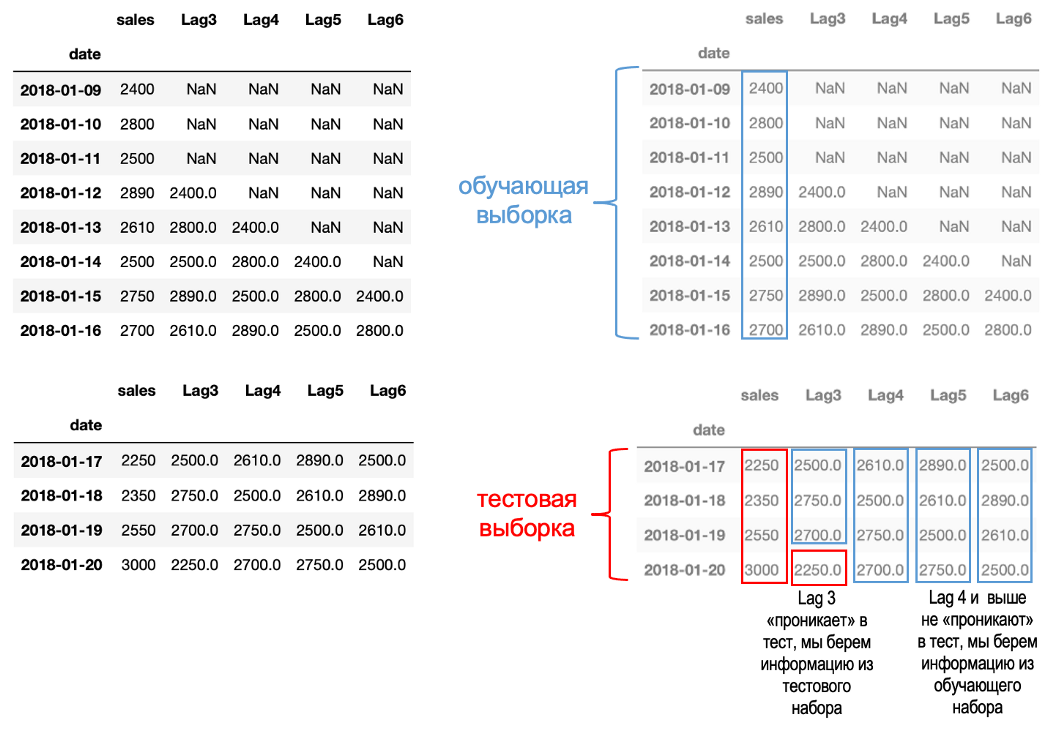
\includegraphics[scale=0.4]{figures/lags.png}
	\caption{ Лаги, у которых порядок равен горизонту прогнозирования или превышает его, не используют тестовую выборку }\label{fig:lags}
\end{figure}



Теперь создадим лаги, скользящее среднее, скользящее среднее абсолютное отклонение, обучим модель \texttt{LGBMModelMultiSegment}, получим прогнозы и визуализируем их
\begin{lstlisting}[
style = ironpython,
numbers = none,
]
# создаем экземпляр класса LagTransform для генерации лагов,
# с помощью in_column задаем переменную, на основе которой
# генерируем лаги, мы будем генерировать лаги порядка от 8 до 23, 
# порядок лагов не должен быть меньше длины горизонта
lags = LagTransform(in_column='target', 
				lags=list(range(8, 24, 1)), 
				out_column='lag')
# создаем экземпляр класса MeanTransform для вычисления 
# скользящего среднего по заданному окну
mean8 = MeanTransform(in_column='target', 
				window=8, 
				out_column='mean8')
# создаем экземпляр класса MadTransform для вычисления 
# среднего абсолютного отклонения по заданному окну
mad8 = MadTransform(in_column='target',
				window=8, 
				out_column='mad8')
# добавляем лаги, mean8, mad8 в обучающую выборку
train_ts.fit_transform([lags, mean8, mad8])
# создаем экземпляр класса LGBMModelPerSegment
model = LGBMModelPerSegment()
# обучаем модель
model.fit(train_ts)
# формируем тестовый набор
future_ts = train_ts.make_future(HORIZON)
# получаем прогнозы
forecast_ts = model.forecast(future_ts)
# оцениваем качество прогнозов
smape(y_true=test_ts, y_pred=forecast_ts)
\end{lstlisting}

\subsection{Работа с несколькими временными рядами}

Прогнозирование нескольких временных рядов. Загрузим набор, в котором каждому сегменту соответствует свой временной ряд
\begin{lstlisting}[
style = ironpython,
numbers = none	
]
original_df = pd.read_csv("data.csv")
original_df.head()

df = TSDataset.to_dataset(original_df)
\end{lstlisting}

Вновь воспользуемся моделью CatBoost с помощью класса CatBoostModelMultiSegment. Перед построением модели выполним некоторые преобразования и создадим новые признаки для наших рядов.

Нам понадобятся следующие классы-трансформеры:
\begin{itemize}
	\item класс \texttt{LogTransform} для логарифмирования и экспонецирования перерменной (логарифмирование позволяет сгладить негативное влияние выборосов объективной природы, помогает выделить тренд),
	
	\item \texttt{LinearTrendTransform} для прогнозирования тренда, удаления тренда из данных и добавления тренда к прогнозам (это необходимо для деревьев решений и для ансамблей деревьев решений, \underline{\emph{не умещющих экстраполировать}}),
	
	\item \texttt{LagTransform} для генерации лагов,
	
	\item \texttt{DateFlagsTransform} для генерации признаков на основе дат -- порядковый номер дня недели, порядковый номер дня месяца, порядковый номер недели в месяце и пр.,
	
	\item \texttt{MeanTransform} для вычисления скользящего среднего по заданному окну.
\end{itemize}

Сначала выполним логарифмирование зависимой переменной, а затем вычтем из нее тренд. Потом на основе пролагрифмированной зависимой переменной с удаленным трендом мы создадим лаги и скользящие средние, добавим календарные признаки.

\begin{lstlisting}[
style = ironpython,
numbers = none
]
# создаем экземпляр класса LogTransform для логарифмирования 
# и экспоненцирования зависимой переменной
log = LogTransform(in_column='target')

# создаем экземпляр класса LinearTrendTransform 
# для прогнозирования тренда, удаления тренда из 
# данных и добавления тренда к прогнозам
trend = LinearTrendTransform(in_column='target')

# создаем экземпляр класса SegmentEncoderTransform 
# для кодирования меток сегментов целочисленными 
# значениями в лексикографическом порядке (LabelEncoding): 
# сегменты a, b, c, d получат значения 0, 1, 2, 3
seg = SegmentEncoderTransform()

# создаем экземпляр класса LagTransform 
# для генерации лагов (c лага 31 по лаг 95)
lags = LagTransform(in_column='target', 
	lags=list(range(31, 96, 1)), 
	out_column='lag')
	
# создаем экземпляр класса DateFlagsTransform для 
# генерации признаков на основе дат - порядковый 
# номер дня недели, порядковый номер дня месяца,
# порядковый номер недели в месяце, порядковый 
# номер недели в году, порядковый номер месяца 
# в году, индикатор выходных дней
d_flags = DateFlagsTransform(day_number_in_week=True,
	day_number_in_month=True,
	week_number_in_month=True,
	week_number_in_year=True,
	month_number_in_year=True,
	special_days_in_week=[5, 6], 
	out_column='datetime')
	
# создаем экземпляр класса MeanTransform для вычисления 
# скользящего среднего по заданному окну
mean30 = MeanTransform(in_column='target', 
	window=30, 
	out_column='mean30')
\end{lstlisting}

Разбиваем набор (наш объект TSDataset) на обучающую и тестовую выборки с учетом временной структуры. Здесь горизонт прогнозирования сосавит 31 день
\begin{lstlisting}[
style = ironpython,
numbers = none
]
# разбиваем набор на обучающую и тестовую выборки 
# с учетом временной структуры
train_ts, test_ts = ts.train_test_split(
    train_start="2019-01-01",
    train_end="2019-11-30",
    test_start="2019-12-01",
    test_end="2019-12-31",
)

# выполняем преобразования набора
train_ts.fit_transform([
	log,  # логарифмируем
	trend,  # удаляем тренд
	lags,  # вычисляем лаги
	d_flags,  # вычисляем признаки на основе дат
	seg,  # кодируем метки сегментов
	mean30  # вычисляем скользящее среднее
])
\end{lstlisting}

Задаем явно горизонт в 31 день, обучаем модель CatBoost, оцениваем качество прогнозов и визуализируем прогнозы. Кроме того, не забываем выполнить обратные преобразования (добавление тренда, экспонецирование зависимой переменной) с помощью метода \texttt{.inverse\_transform()} для обучающего набора для правильной визуализации значений зависимой переменной в обучающей выборке.

\begin{lstlisting}[
style = ironpython,
numbers = none
]
# задаем горизонт прогнозирования
HORIZON = 31
# создаем экземпляр класса CatBoostModelMultiSegment
model = CatBoostModelMultiSegment()
# обучаем модель CatBoost
model.fit(train_ts)
# формируем набор, для которого нужно получить прогнозы,
# длина набора определяется горизонтом прогнозирования
future_ts = train_ts.make_future(HORIZON)

# получаем прогнозы
forecast_ts = model.forecast(future_ts)

# оцениваем качество прогнозов
smape(y_true=test_ts, y_pred=forecast_ts)
\end{lstlisting}

Выполняем обратное преобразование для обратной выборки (добавляем тренд, делаем экспоненцирование переменной \texttt{target})
\begin{lstlisting}[
style = ironpython,
numbers = none
]
train_ts.inverse_transform()
plot_forecast(forecast_ts, test_ts, train_ts, n_train_sample=20)
\end{lstlisting}

Для более надежной оценки качества модели \texttt{CatBoost} воспользуемся \emph{перекрестной проверкой расширяющимся окном}
\begin{lstlisting}[
style = ironpython,
numbers = none
]
pipe = Pipeline(
    model=model,
    transform=[
        log,
        trend,
        seg,
        lags,
        d_flags,
        mean30,
    ],
    horizon=HORIZON,
)
metrics, forecast, info = pipe.backtest(ts, [smape], aggregate_metrics=True)
\end{lstlisting}

Ансамбль бустингов
\begin{lstlisting}[
style = ironpython,
numbers = none,
]
transforms = [log, trend, seg, lags, d_flags, mean30]
catboost_pipeline = Pipeline(
    model=CatBoostModelMultiSegment(),
    transforms=transforms,
    horizon=HORIZON
)

lightgbm_pipeline = Pipeline(
    model=LGBMModelMultiSegment(),
    transforms=transforms,
    horizon=HORIZON
)

xgboost_pipeline = Pipeline(
    model=XGBModelMultiSegment(learning_rate=0.2, n_estimators=500, max_depth=1),
    transforms=transforms,
    horizon=HORIZON
)

pipeline_names = ["catboost", "lightgbm", "xgboost"]
pipelines = [catboost_pipeline, lightgbm_pipeline, xgboost_pipeline]

voting_ensemble = VotingEnsemble(
    pipelines=pipelines,
    weight=[1, 1, 2],
    n_jobs=1
)

metrics, forecast, _ = voting_ensemble.backtest(
    ts=ts, metrics=[SMAPE()], n_folds=3, aggregate_metrics=True, n_jobs=1
)
\end{lstlisting}

Заметим, что скользящее среднее используется не только для конструирования признаков, но и в качестве прогнозной модели (когда прогноз -- скользящее среднее $ n $ последних наблюдений), а также для сглаживания выборосов, краткосрочных колебаний и более четкого выделения долгосрочных тенденций в ряде данных.

\section{Генерация признаков и кодирование категориальных признаков}

Процесс создания признакового пространства зависит от модели, которую будем использовать:
\begin{itemize}
	\item OHE-кодирование предпочтительнее для линейных моделей,
	
	\item умное кодирование категорий -- для деревьев,
	
	\item выбросы можно не удалять для робастной модели.
\end{itemize}

Если в тестовом наборе данных присутствуют категории, которых не было в обучающем наборе данных, то нужно принять решение о том, как их кодировать. Например, категорию из нового набора данных можно отнести к самомой опасной категории из тех, категорий, которые присутствуют в обучающем наборе данных.

Еще категории можно кодировать по разным признакам.

Можно кодировать признаки по мощности (Count Encoding): сколько раз каждая уникальная категория встречалась в категориальном признаке. Проблема в том, что некоторые категории могут встречаться одинаковое количество раз (коллизия). Чтобы различать такие категории можно добавить шум, т.е. $ count + \varepsilon $. Мелкие и новые категории объединяют в одну.

Кодирование по мощности можно использовать, если требуется быстро решить задачу.

\subsection{Кодирование одного категориального признака по другому категориальному признаку с помощью сингулярного разложения}

Если матрица признакового описания объекта состоит только из категориальных признаков, то можно кодировать один признак на основе другого
\begin{lstlisting}[
style = ironpython,
numbers = none
]
from numpy.linalg import svd

def code_factor(data, cat_feature, cat_feature2):
    """
    Кодирование признака на основе другого признака
    """
    ct = pd.crosstab(data[cat_feature], data[cat_feature2])
    u, _, _ = svd(ct.values)
    coder = dict(zip(ct.index, u[:, 0]))  # берем только первый сингулярный вектор
    
    return data[cat_feature].map(coder)
\end{lstlisting}

Сингулярное разложение (Singular Value Decomposition, SVD) -- декомпозиция вещественной матрицы с целью ее приведения к каноническому виду. Сингулярное разложение является удобным методом при работе с матрицами. Оно показывает геометрическую структуру матрицы и позволяет наглядно представить имеющиеся данные. В числе прочего SVD позволяет вычислять обратные и псевдообратные матрицы большого размера, что делает его полезным инструментом при решении задач регрессионного анализа.

\remark{
В числе прочего с помощью сингулярного разложения можно решать задачи обращения или пвседообращения матриц большого размера
}

Для любой вещественной $ (n \times n) $-матрицы $ A $ существуют две вещественные ортогональные $ (n \times n) $-матрицы $ U $ и $ V $ такие, что
\begin{align*}
	\Lambda = U^{T} A V,
\end{align*}
где $ \Lambda $ -- диагональная матрица.

Матрицы $ U $ и $ V $ выбираются так, чтобы диагональные элементы матрицы $ A $ имели вид
\begin{align*}
	\lambda_1 \geqslant \lambda_2 \geqslant \ldots \geqslant \lambda_r > \lambda_{r + 1} = \lambda_n = 0,
\end{align*}
где $ r $ -- ранг матрицы $ A $.

В частности, если $ A $ невырождена (то есть существует обратная матрица $ A^{-1}, \det A \neq 0 $), то
\begin{align*}
	\lambda_1 \geqslant \lambda_2 \geqslant \ldots \geqslant \lambda_n > 0.
\end{align*}

\underline{Столбцы} матриц $ U $ и $ V $ называются соответсвенно \emph{левыми} и \emph{правыми сингулярными векторами}, а значения диагонали матрицы $ \Lambda $ -- \emph{сингулярными числами}.

Эквивалентная запись сингулярного разложения
\begin{align*}
	A = U \Lambda V^{T}
\end{align*}

Например, матрица
\begin{align*}
	A = \begin{pmatrix}
		0.96 & 1.72 \\
		2.28 & 0.96
	\end{pmatrix}
\end{align*}
имеет сингулярное разложение
\begin{align*}
	A = U \Lambda V^{T} =
	\begin{pmatrix}
		0.6 & 0.8\\
		0.8 & -0.6
	\end{pmatrix}
    \begin{pmatrix}
    	3 & 0\\
    	0 & 1
    \end{pmatrix}
    \begin{pmatrix}
    	0.8 & -0.6 \\
    	0.6 & 0.8
    \end{pmatrix}^T
\end{align*}

Легко увидеть, что матрицы $ U $ и $ V $ ортогональны,
\begin{align*}
	U^T U = UU^T = I, \quad V^T V = V V^T = I,
\end{align*}
и сумма квадратов значений их столбцов равна единице.

Для \emph{прямоугольных} матриц существует так называемое экономное представление сигнулярного разложения
\begin{align*}
	A_{(m \times n)} = U_{(m \times r)} \Lambda_{(r \times r)} V_{(r \times n)}^T,
\end{align*}
где $ r = \min(m, n) $.

\noindent\emph{Сингулярное разложение и собственные числа матрицы}

Сингулярное разложение обладает свойством, которое связывает задачу отыскания сингулярного разложения и задачу отыскания собственных векторов. Собственный вектор $ x $ матрицы $ A $ -- такой вектор, при котором выполняется условие $ A x = \lambda x $, где $ \lambda $ -- собственное число.

Так как матрицы $ U $ и $ V $ ортогональные, то
\begin{align*}
	A A^T = U \Lambda \underbrace{V^T V}_{= I} \Lambda U^T = U \Lambda^2 U^T,\\
	A^T A = V \Lambda \underbrace{U^T U}_{= I} \Lambda V^T = V \Lambda^2 V^T.
\end{align*}

Умножая оба выражения справа соответсвенно на $ U $ и $ V $, получаем
\begin{align*}
	A A^T U = U \Lambda^2,\\
	A^T A V = V\Lambda^2.
\end{align*}

Из этого следует, что \underline{столбцы} матрицы $ U $ являются собственными векторами матрицы $ AA^T $, а квадраты сингулярных чисел $ \Lambda = \text{diag}(\lambda_1, \ldots, \lambda_r) $ -- ее собственным числам. Также \underline{столбцы} матрицы $ V $ являются собственными векторами матрицы $ A A^T $, а квадраты сингулярных чисел являются ее собвственными числами.

\noindent\emph{SVD и норма матриц}

Евклидова норма
\begin{align*}
	|A|_E = \max\limits_{|x| = 1} \dfrac{ |A x| }{ |x| }.
\end{align*}

Норма Фробениуса
\begin{align*}
	|A|_F = \sqrt{\sum_{i=1}^{m}\sum_{j=1}^{n} a_{ij}^2}.
\end{align*}

Если известно сингулярное разложение, то обе эти нормы легко вычислить. Пусть $ \lambda_1, \ldots, \lambda_r $ -- сингулярные числа матрцы $ A $, отличные от нуля.

Тогда $ |A|_E = \lambda_1 $ и $ |A|_F = \sqrt{\sum\limits_{k=1}^{r} \lambda_k^2} $.

\noindent\emph{Нахождение псевдообратной матрицы с помощью SVD}

Если $ (m \times n) $-матрица $ A $ является \emph{вырожденной} или \emph{прямоугольной}, то обратной матрицы $ A^{-1} $ для нее \underline{не существует}. 

Однако, для $ A $ может быть найдена псевдообратная матрица $ A^{+} $ -- такая матрица, для которой выполняются условия
\begin{align*}
	A^{+}A &= I_n,\\
	A A^{+} &= I_m,\\
	A^{+} A A^{+} &= A^{+},\\
	A A^{+} A &= A.
\end{align*}

Пусть найдено разложение матрицы $ A $ вида
\begin{align*}
	A = U \Lambda V^T,
\end{align*}
где $ \Lambda = \text{diag}(\lambda_1, \ldots, \lambda_r), r=\min(m, n) $ и $ U^T U = I_m, VV^T = I_n $.

Тогда матрица
\begin{align*}
	A^+ = V^T \Lambda^{-1}U
\end{align*}
является для матрицы $ A $ \emph{псевдообратной}.

\noindent\emph{Усеченное SVD при обращении матриц}

Для получения обращения, устойчивого к малым изменениям значений матрицы $ A $, используется усеченное SVD. Пусть матрица $ A $ представлена в виде $ A = U\Lambda V^T $.

Тогда \emph{усеченная псевдообратная матрица} $ A_s^+ $
\begin{align*}
	A_s^+ = V \Lambda_s^{-1} U^T,
\end{align*}
где $ \Lambda_s^{-1} = \text{diag}(\lambda_1^{-1}, \ldots, \lambda_s^{-1}, 0, \ldots, 0) $ -- $ (n \times n) $-диагональная матрица, $ s $ -- первые $ s $ сингулярных чисел, $ s \leqslant \text{rang} A $.

Есть еще хэш-кодирование (\texttt{sklearn.feature\_extractoin.FeatureHasher}). Для быстрого анализа пойдет, но применяется редко.

Можно кодировать категории по целевой переменной (Target Encoding). Есть варианты целевого кодирования по среднему (Mean Target Encoding), по стандартному отклонению (Std Target Enconing) и т.д. Подход для \emph{любого} алгоритма. Кодирование по значению целевой переменной <<логично>>.

Главная проблема: неадекватная кодировка мелких категорий + слияние этих категорий. Нельзя допустить утечки значений целевой переменой!

Теоретически можно кодировать категориальные признаки на обучающем поднаборе, а обучать алгоритм на отложенной выборке, но это не очень здорово, так как теряем значительную часть данных на этапе кодирования.

Кодирование по \emph{предыдущим} объектам (CatBoost). Одна категория в обучении кодируется по-разному, а на контроле фиксировано
\begin{lstlisting}[
style = ironpython,
numbers = none	
]
gb = data.groupby(name)
data[name + "_cb"] = (gb["target"].cumsum() - data["target"]) / gb.cumcount()
\end{lstlisting}

Получаются более менее адекватные значения, но без подглядывания. В самом начале кодирования (в первых строках) пока статистика не наберется значения будут неадекватные. Можно тасовать матрицу признакового описания объекта, а затем усреднять результаты кодировки.

На практике хорошо работает смесь подходов!


\section{Перестановочная важность признаков и важность признаков по Шепли}

Полезный ресурс \url{https://scikit-learn.org/stable/modules/permutation_importance.html}

Статья Дьяконова \href{https://dyakonov.org/2018/08/28/%d0%b8%d0%bd%d1%82%d0%b5%d1%80%d0%bf%d1%80%d0%b5%d1%82%d0%b0%d1%86%d0%b8%d0%b8-%d1%87%d1%91%d1%80%d0%bd%d1%8b%d1%85-%d1%8f%d1%89%d0%b8%d0%ba%d0%be%d0%b2/}{про интерпретацию черных ящиков}

Важность признаков -- числовые оценки, насколько каждый признак \emph{важен} для решения поставленной задачи.

{\color{red} Плохой метод -- чем чаще выбирался признак, тем лучше.} Дело в том, что признак может действительно часто выбираться, но на более низких уровнях дерева (дальше от корня). Другими словами, признак выбирается часто, но используется для построения небольших <<уточняющих>> разбиений (\pic{fig:feature_imp}). Как правило, все наоборот. Если признак выбирается часто, значит модель не может по каким-то причинам сразу получить от него нужную информацию.

\begin{figure}[h]
	\centering
	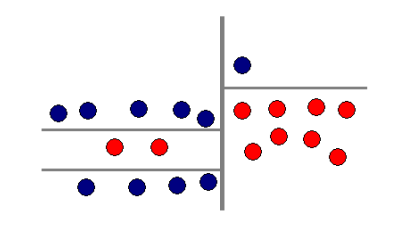
\includegraphics[scale=1.]{figures/feature_imp.png}
	\caption{ К вопросу о важности признака по частоте его выбора. Признак по оси $ x $ выбирается только один раз, а признак по оси $ y $ выбирается три раза, но очевидно, что первый признак лучше справляется с задачей }\label{fig:feature_imp}
\end{figure}

{\color{red}Нельзя отбрасывать признаки по порогу.}

Перестановочная важность признаков и важность признаков по Шепли обладают свойством \emph{согласованности} (если модель изменить так, что она более существенно начинает зависеть от какого-то признака, то его важность не убывает).

Подход вычисления \textbf{\itshape перестановочной важности признаков} (Permutation Feature Importance):
\begin{itemize}
	\item (+) не меняет распределение по конкретному признаку (так как рассматриваемый признак просто перемешивается),
	
	\item (+) не требует обучать модель заново -- обученную модель тестируют на \emph{\color{red}отложенной} выборке с \emph{\color{red}испорченным} признаком; то есть исходный набор данных разбивается на обучение и тест, модель обучается на обучающем поднаборе данных, на тестовом поднаборе мы вычисляем качество модели без модификации признаков, затем перетасовываем какой-то признак тестового поднабора и вычисляем качество на тестовом поднаборе с испорченным признаком, а затем делаем вывод о том на сколько качество изменилось (на сколько признак важен); Модель для вычисления важности признаков обучается на обучающем поднаборе данных, а \emph{важность признаков} вычисляется на \emph{\color{red}отложенной выборке}, включая различные схемы валидации; то есть можно было бы разбить исходный набор данных на $ k $ фолдов: обучаемся на $ k - 1 $ фолдах, вычисляем качество на \emph{валидационном} поднаборе данных без модификации признаков, затем применяем ту же самую модель (обученную на обучающем поднаборе данных первого разбиения) к валиадционному поднабору, но с уже перетасованным $ i $-ым признаком; и так поступаем для всех признаков $ f $ каждого фолда; теперь можно усреднить результаты по фолдам; в итоге мы получим $ f $ усредненных по фолдам важностей признаков,
	
	\item (+) можно применять на любых алгоритмах,
	
	\item (+) самый надежный метод,
	
	\item (+) в бутсрепе можно использовать OOB-контроль (строить дерево и на зкземплярах, не попавших в дерево, вычислять перестрановочную важность),
	
	\item (-) очень медленный.
\end{itemize}

\remark{
Вместо метрик качества для вычисления перестановочной важности можно использовать что-то другое. Например, долю верно классифицирующих деревьев
}

Идея перестановочной важности признаков: признак важный, если его перетасовка снижает качество. Можно вычислять перестановочную важность признаков на \emph{обучающем поднаборе данных} (вроде как бы можно, но лучше использовать отложенную выборку PFI-holdout), на \emph{отложенном контроле} (тестовый поднабор данных PFI-holdout, \pic{fig:PFI-holdout}) и на любой схеме \emph{валидации} (надежнее использовать валидацию). 

\begin{figure}[h]
	\centering
	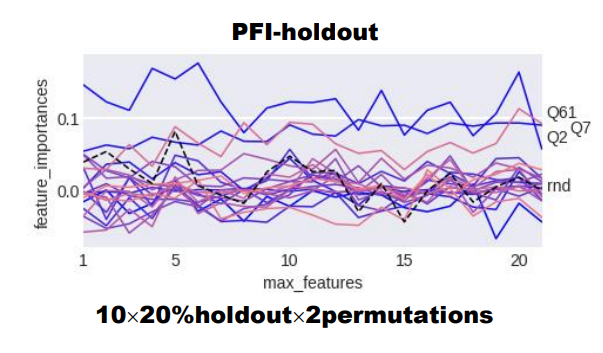
\includegraphics[scale=1.]{figures/PFI-holdout.png}
	\caption{ Перестановочная важность признаков, вычисленная на отложенной выборке }\label{fig:PFI-holdout}
\end{figure}

Перестановочная важность скоррелиррованных признаков может размазываться между ними.

Можно удалять признаки (Drop-column importance), но тогда каждый раз нужно будет заново обучать модель. Однако при этом результат более однозначный. Используется редко!

Если два признак коррелируют друг с другом, то перестановка одного из них не будет значимо сказываться на эффективности модели, потому что она может извлечь требуемую информацию из второго коррелирующего признака. Одним из способов работы с мультиколлинеарными признаками является иерархическая кластеризация на базе ранговых корреляций Спирмена, выбор порога отсечения и сохранение одного признака из каждого кластера.

\remark{
Важности признаков, полученные с помощью \texttt{feature\_importances\_} (важность по неоднородности), встроенного в алгоритмы построения ансамблей деревьев -- это НЕ важности признаков для решения задачи, а лишь для настройки конкретной модели. Этот подход не обладает свойством согласованности!!!}

В разделе 4.2.2 Relation to impurity-based importance in trees документации sklearn говорится, что impurity-based importance (\emph{важность признаков по неоднородности}; еще называют Gini importance) сильно смещена и отдает предпочтение \underline{высококардинальным} признакам (обычно вещественным) по сравнению с низкокардинальными признаками, такими как бинарные или категориальные признаки с небольшим числом категорий. Кроме того, важность по неоднородности годится только для деревьев и их ансамблей.

\textbf{\emph{Важность по Шепли}} $ i $-ого признака вычисляется следующим образом
\begin{align*}
	\varphi_i = \sum_{S \subseteq \{1, 2, \ldots, n\} \setminus \{i\}} \dfrac{ | S |! (n - |S| - 1)! }{ n! } \big( f(S \cup \{i\}) - f(S) \big),
\end{align*}
где $ f(S) $ -- ответ модели, обученной на подмножестве $ S $ множества $ n $ признаков (на конкретном объекте -- вся формула записывается для конкретного объекта).

Вычисление требует переобучения модели на всевозможных подмножествах признаков, поэтому на практике применяются приближения формулы, например, с помощью метода Монте-Карло.

Замечания по методам оценки важности признаков:
\begin{itemize}
	\item \underline{\itshape нет идеального алгоритма оценки важности признаков} (для любого можно подобрать пример, когда он плохо работает),
	
	\item если много похожих признаков (например, сильно коррелированных), то важность может <<делиться между ними>>, поэтому не рекомендуется отбрасывать признаки по порогу важности,
	
	\item есть старая рекомендация (впрочем, без теоретического обоснования): модель для решения задачи и оценки важности должны основываться на разных парадигмах (например, оценивать важность с помощью случайного леса и потом настраивать его же на важных признаках не рекомендуется). {\color{blue}То есть не рекомендуется оценивать важность и решать ML-задачу одним и тем же алгоритмом!!!}
\end{itemize}

Советы Дьяконова:
\begin{itemize}
	\item можно выбрать некоторое подмножество признаков и потом то добавить $ k $ признаков, то отнять $ l $,
	
	\item оценивать важность не обязательно с помощью лучшей модели (то есть не нужно строить супермодель для того, чтобы оценить важность признаков!)
	
	\item перестановочная важность самая естественная (но есть нюансы: коррелированность признаков, стабильность оценки и т.п.),
	
	\item есть и другие подходы и удобные библиотеки (SHAP, например).
\end{itemize}

\section{Приемы работы с библиотекой Polars}

\subsection{Уствновка}

Установить библиотеку Polars \url{https://www.pola.rs/} можно с помощью мендежера пакетов \texttt{pip}
\begin{lstlisting}[
style = ironpython,
numbers = none
]
pip install polars
\end{lstlisting}

С библиотекой Polars удобнее работать, использую оболочку \texttt{ptpython}.

\subsection{Вводные замечания}

Polars поддерживает режимы \emph{жадных} (eager)\footnote{В этом режиме работа с данными выглядит как в pandas} и \emph{отложенных} (lazy) вычислений.

Пример
\begin{lstlisting}[
style = ironpython,
numbers = none	
]
import polars as pl

df = pl.read_csv("https://j.mp/iriscsv")
print(
	df.filter(pl.col("sepal_length") > 5)
	.groupby("species")
	.agg(pl.all().sum())
)
\end{lstlisting}

Или в <<отложенном>> режиме
\begin{lstlisting}[
style = ironpython,
numbers = none
]
import polars as pl

print(
	pl.read_csv("https://j.mp/iriscsv")
	.lazy()  # набор данных сразу не загружается!
	.filter(pl.col("sepal_length") > 5)
	.groupby("species")
	.agg(pl.all().sum())
	.collect()
)
\end{lstlisting}

На Pandas этот запрос выглядел бы так
\begin{lstlisting}[
style = ironpython,
numbers = none
]
import numpy as np
import pandas as pd

df = pd.read_csv("https://j.mp/iriscsv")
df.loc[df.loc[:, "sepal_length"] > 5].groupby("species").agg(np.sum)
\end{lstlisting}

Если набор данных храниться \underline{\itshape локально}, то можно воспользоваться семейством функций \texttt{scan\_**}
\begin{lstlisting}[
style = ironpython,
numbers = none
]
pl.scan_csv("./iris.csv").\
    select(["sepal_width", "petal_width"]).\
    filter(pl.col("sepal_width") > 3.5).\
    collect()
\end{lstlisting}

Lazy API создает план выполнения запроса. Никакой шаг пайплайна не выполняется пока мы явно попросим Polars выполнить запрос (с помощью \verb*|LazyFrame.collect()| или \verb*|LazyFrame.fetch()|). Этот прием дает возможность Polars проанализировать весь запрос и выбрать наиболее подходящий по контексту алгоритм вычислений.


Чтобы перейти от жадного режима к ленивому достаточно просто начать запрос с \verb*|.lazy()|, а закончить \verb*|.collect()|.

\subsection{Polars-выражения}

Метод \texttt{filter} отбирает строки, а метод \texttt{select} -- столбцы.

Polars поддерживает очень мощную концепцию выражений. Рассмотрим несколько примеров
\begin{lstlisting}[
style = ironpython,
numbers = none,
]
out = df.select([
    pl.col("name").n_unique().alias("unique_names_1"),
    pl.col("name").unique().count().alias("unique_names_2")
])
\end{lstlisting}

Можно вызывать различные агрегаторы на объекте солбца
\begin{lstlisting}[
style = ironpython,
numbers = none
]
df.select(pl.col("name").std())
df.select(pl.col("name").max())
\end{lstlisting}

Можно выбирать столбцы по регулярному выражению
\begin{lstlisting}[
style = ironpython,
numbers = none
]
df.select(r"^Type\s{1}\d{1}$")  # выбирет столбцы 'Type 1', 'Type 2' etc.
\end{lstlisting}

Можно использовать фильтры и условия. В фильтр передается булева маска
\begin{lstlisting}[
style = ironpython,
numbers = none
]
df.select([
    pl.col("species").filter(
        pl.col("species").str.contains(r".*osa$")
    ).count() # count() -- это метод объекта столбца
])  # 50
\end{lstlisting}

На Pandas этот запрос выглядел бы так
\begin{lstlisting}[
style = ironpython,
numbers = none
]
df.loc[
    df.loc[:, "species"].str.contains(r".*osa$")  # вернет булеву маску
]["species"].count()  # 50

# или так
df.loc[
    df.loc[:, "species"].str.contains(r".*osa$")  # вернет булеву маску
].shape[0]  # 50
\end{lstlisting}

Можно использовать конструкцию \emph{when} $ \rightarrow $ \emph{then} $ \rightarrow $ \emph{otherwise}
\begin{lstlisting}[
style = ironpython,
numbers = none	
]
df.select([
    pl.when(pl.col("petal_length") > 3)
    .then(100)
    .otherwise(pl.col("sepal_width") * 10) * pl.col("sepal_length").sum()
])
\end{lstlisting}

На Pandas запрос выглядел бы так
\begin{lstlisting}[
style = ironpython,
numbers = none
]
np.where(
    df.loc[:, "petal_length"] > 3,
    100,
    df.loc[:, "sepal_width"] * 10
) * df.loc[:, "sepal_length"].sum()
\end{lstlisting}

Еще пример
\begin{lstlisting}[
style = ironpython,
numbers = none
]
# Polars
(
    df
    .lazy()
    .groupby("species")
    .agg(pl.all().sum())
    .select(["species", "petal_length"])
    .collect()
)

# Pandas
(
    df
    .groupby("species")
    .agg(np.sum)[["species", "petal_lenth"]]
)
\end{lstlisting}

Пример группировки с последующим построением агрегата
\begin{lstlisting}[
style = ironpython,
numbers = none
]
df.groupby("species").agg([
    pl.col("sepal_width").mean(),
    pl.col("petal_length").max(),
]).sort("species")
\end{lstlisting}

На Pandas
\begin{lstlisting}[
style = ironpython,
numbers = none
]
df.groupby("species").agg({
    "sepal_width": np.mean,
    "petal_length": np.max,
}).sort_index()
\end{lstlisting}

Если нужны склеить поэлементно строковые столбцы, то лучше воспользоваться функцией \verb*|pl.concat_str([...])|, а не fold-выражением, так как из-за материализации промежуточных столбцов у fold-выражений будет квадратичная временная сложность
\begin{lstlisting}[
style = ironpython,
numbers = none
]
df.select([
    pl.concat_str(["a", "b"])  # "a" и "b" это имена столбцов
])
\end{lstlisting}

Polars-выражения нельзя использовать везде. Вот допустимые \emph{контексты}:
\begin{itemize}
	\item \verb*|df.select([...])|
	
	\item \verb*|df.groupby(...).agg([...])|
	
	\item \verb*|df.with_columns([...])|
\end{itemize}

Даже в тех случаях, когда мы явно работаем в <<жадном>> режиме, на самом деле используется режим отложенных вычислений
\begin{lstlisting}[
style = ironpython,
numbers = none
]
df.groupby("foo").agg([pl.col("bar").sum()])
# на самом деле
(df.lazy().groupby("foo").agg([pl.col("bar").sum()])).collect()
\end{lstlisting}

Добавить столбец (или несколько столбцов) можно так
\begin{lstlisting}[
style = ironpython,
numbers = none
]
df.with_columns([
    (pl.col("sepal_length").sum() + pl.col("petal_width")).alias("new_col_1"),
    pl.col("sepal_length").mean().alias("new_col_2")
])
\end{lstlisting}

Создать производный столбец с кастомной функцией можно так
\begin{lstlisting}[
style = ironpython,
numbers = none
]
df.with_columns([
    pl.col("Speed").map(f=lambda elem: elem ** 2).alias("SquaredSpeed")
])
\end{lstlisting}

Если псевдоним не задать, то метод \verb*|with_columns| перезапишет существующий столбец \texttt{"Speed"}. Но \verb*|with_columns| возвращает новый объект.

\remark{
\color{red}
Пользовательские Python-функции убивают распараллеливание!
}

Можно также фильтровать группы. Пусть требуется вычислить среднее по группе, но не для всех элементов группы. Для ясности можно использовать Python-функции. Они ничего не стоят, потому как применяются только в Polars-выражении, а на шаге выполнения запроса
\begin{lstlisting}[
style = ironpython,
numbers = none	
]
from datetime import date

import polars as pl

from .dataset import dataset


def compute_age() -> pl.Expr:
	return date(2021, 1, 1).year - pl.col("birthday").dt.year()


# здесь мы вычисляем временную дельту для столбца 'birthday',
# а фильтруем по ассоциированным строкам столбца 'gender'
def avg_birthday(gender: str) -> pl.Expr:
	return compute_age().filter(pl.col("gender") == gender).mean().alias(f"avg {gender} birthday")


q = (
	dataset.lazy()
	.groupby(["state"])
	.agg(
		[
			avg_birthday("M"),
			avg_birthday("F"),
			(pl.col("gender") == "M").sum().alias("# male"),
			(pl.col("gender") == "F").sum().alias("# female"),
		]
	)
	.limit(5)
)

df = q.collect()
\end{lstlisting}

С помощью метода \texttt{filter} мы отбираем строки в столбце \texttt{'gender'}, а затем по оставшимся строкам столбца \texttt{'gender'} вычисляем среднее и связываем результат с псевдонимом.

Еще вместо группировки можно использовать фильтр по одному столбцу и агрегацию по другому столбцу
\begin{lstlisting}[
style = ironpython,
numbers = none	
]
df.select([
    pl.col("sepal_width").filter(pl.col("species") == "setosa").mean()
])  # 3.418
\end{lstlisting}

На Pandas было бы так
\begin{lstlisting}[
style = ironpython,
numbers = none	
]
df.loc[df.loc[:, "species"] == "setosa", "sepal_width"].mean()
\end{lstlisting}

\subsection{Оконные функции}

Оконную функцию из обычной можно сделать, вызвав метод $ \verb*|.over()| $.

Пример
\begin{lstlisting}[
style = ironpython,
numbers = none	
]
df.select(["Type 1", "Type 2", "Attack", "Defense"]).select([
	"Type 1",
	"Type 2",
	pl.col("Attack").mean().over("Type 1").alias("avg_attack_by_type"),
	pl.col("Defense").mean().over(["Type 1", "Type 2"]).alias("avg_defense_by_type_comb"),
])
\end{lstlisting}

Добавить столбец \texttt{"WinCumsum"} с кумулятивной суммой по группе
\begin{lstlisting}[
style = ironpython,
numbers = none	
]
df.select([
    "Type 1",
    "Speed",
    pl.col("Speed").cumsum().over("Type 1").alias("WinCumsum"),
]).sort("Type 1")
\end{lstlisting}

Еще пример оконной функции. NB: столбцы, которые используются в \verb*|.over([...])| должны быть отсортированы
\begin{lstlisting}[
style = ironpython,
numbers = none	
]
df.sort("Type 1").select([
    pl.col("Type 1").head(3).list().over("Type 1").flatten(),
    pl.col("Name").sort_by("Attack").head(3).list().over("Type 1").flatten().alias("fastest/group"),
    pl.col("Name").sort_by(pl.col("Speed")).head(3).list().over("Type 1").flatten().alias("strongest/group"),
])
\end{lstlisting}

\subsection{Универсальные NumPy-функции}

Polars поддерживает универсальные numpy-функции \verb*|ufuncs| \url{https://numpy.org/doc/stable/reference/ufuncs.html#available-ufuncs}.

Пример
\begin{lstlisting}[
style = ironpython,
numbers = none
]
df.select([
    np.log(pl.all()).suffix("_log")  # pl.all() -- применяется ко всем столбцам
])
\end{lstlisting}

\subsection{Примеры}

Столбцы можно выбирать по регулярному выражению
\begin{lstlisting}[
style = ironpython,
numbers = none
]
df.select([
    pl.col(r"^Type\s{1}\d{1}$")  # Polars-выражение
])

# или так
df.select(r"^Type\s{1}\d{1}$")

df.select([
    pl.col(r"^Sp.*$").sum()
])
\end{lstlisting}

С помощью конструкции \texttt{pl.all()} можно выбирать все столбцы в таблице (работает также как \verb*|*| в SQL-запросах)
\begin{lstlisting}[
style = ironpython,
numbers = none
]
df.select([
    pl.all().reverse().suffix("_rev")  # выбрать все столбцы в обратном порядке
])

df.select([
    pl.all().sum().suffix("_sum")  # найти сумму по всем столбцам
])
\end{lstlisting}

Polars-выражения можно связывать с переменными
\begin{lstlisting}[
style = ironpython,
numbers = none
]
mask = pl.col("Type 1").str.contains(r"^Gr.*$")

df.select([
    mask.sum(),  # найти количество элементов, удовлетворяющих шаблону
])

df.select([
    pl.col("Speed").filter(mask).sum(),
])
\end{lstlisting}

Пример с when-then-otherwise
\begin{lstlisting}[
style = ironpython,
numbers = none	
]
df.select([
    "Type 1",
    pl.when(pl.col("Type 1") == "Grass")
    .then(pl.col("Type 2").str.to_uppercase())
    .otherwise(pl.col("Name").str.to_lowercase())
])
\end{lstlisting}

Пример с оконными функциями
\begin{lstlisting}[
style = ironpython,
numbers = none
]
df.select([
    "fruits",
    "cars",
    "B",
    pl.col("B").sum().over("fruits").alias("B_sum_by_fruits"),
    pl.col("B").sum().over("cars").alias("B_sum_by_cars"),
])
\end{lstlisting}

Сумма вычисляется по группе и транслируется на все элементы группы.

Приклеить столбец справа можно с помощью метода \texttt{hstack}
\begin{lstlisting}[
style = ironpython,
numbers = none
]
df: pl.DataFrame
df.hstack([
    pl.Series("new_col", np.random.randint(10, 100, size=df.height))
])
\end{lstlisting}

Вставить столбец в произвольную позицию можно так
\begin{lstlisting}[
style = ironpython,
numbers = none
]
# insert_at_idx изменяет объект на месте
df.insert_at_idx(0, pl.Series("new_col", np.random.randn(df.heigth)))
\end{lstlisting}

\subsection{Работа с временными рядами}

Pandas-конструкцию \verb*|ts.resample(...).agg(...)| силами Polars можно реализовать так
\begin{lstlisting}[
style = ironpython,
numbers = none
]
ts.groupby_dynamic(
    "time_stamp",
    every="4h",
    closed="left",
).agg([
    pl.col("value").count().alias("value_cnt"),
    pl.col("value").mean().suffix("_mean"),
])
\end{lstlisting}


\section{Приемы работы с библиотекой Catboost}

Онлайн документация пакета \url{https://catboost.ai/en/docs/concepts/python-reference_catboostregressor}.

\subsection{Установка CatBoost}

Установить пакет можно с помощью менеджера \texttt{conda} (или с помощью \texttt{pip})
\begin{lstlisting}[
style = bash,
numbers = none
]
$ conda config --show channels
# если канала conda-forge нет в списке, то следует его добавить 
$ conda config --add channels conda-forge
$ conda install catboost
$ pip install catboost
\end{lstlisting}

\subsection{Ключевые особенности пакета}

\subsection{Параметры}

\remark{
Помимо \texttt{iterations} и \texttt{learning\_rate} у CatBoost 5 важнейших гиперпараметров: \texttt{max\_depth}, \texttt{l2\_leaf\_reg}, \texttt{border\_count}, \texttt{random\_strength} и \texttt{bagging\_temperature}
}

Применительно к \texttt{random\_strength} замечено, что часто значение, близкое к 0 (примерно, 0.15), дает лучшее качество. Если переменных много, можно попробовать настраивать \texttt{rsm}.

В случае дисбаланса классов будет полезным настраивать
\begin{itemize}
	\item либо гиперпараметр \texttt{auto\_class\_weights},
	
	\item либо гиперпараметры \texttt{class\_weights} и \texttt{scale\_pos\_weight}
\end{itemize}
при этом не нужно настраивать эти параметры одновременно.

Можно сначала при \emph{небольшом} числе итераций найти оптимальные значения гиперпараметров, \emph{меньше} всего зависящие от количества итераций (речь прежде всего идет об \texttt{auto\_class\_weights}, \texttt{max\_depth}; при этом \texttt{learning\_rate} и \texttt{rsm} зависят от количества итераций, поэтому нам для небольшого количества итераций придется увеличить темп обучения, а варьирование \texttt{rsm} сделать минимальным). Затем можно построить модель с найденными оптимальными значениями гиперпараметров  \texttt{auto\_class\_weights}, \texttt{max\_depth} и \texttt{rsm}, но уже с большим количеством деревьев, при этом, разумеется помня о двух вещах:
\begin{itemize}
	\item при большом количестве итераций нужно уменьшить темп обучения,
	
	\item выбирая меньшее значение \texttt{rsm}, нужно задавать больше итераций.
\end{itemize}

Ознакомится с описанием параметров можно здесь \url{https://catboost.ai/en/docs/references/training-parameters/}

Общие параметры:
\begin{itemize}
	\item \verb|loss_function| (objective) -- функция потерь, которая используется на шаге обучения модели.
	
	\item \texttt{iterations} -- максимальное число деревьев в ансамбле,
	
	\item \verb*|learning_rate| -- темп обучения,
	
	\item \verb*|l2_leaf_reg| -- коэффициент при члене $ L_2 $-регуляризации,
	
	\item \verb*|bagging_temperature| -- задает настройки Байесовского бутстрапа
\end{itemize}



\subsection{Классификатор CatBoostClassfier}

Класс \texttt{CatBoostClassifier}

\begin{lstlisting}[
style = ironpython,
numbers = none	
]
class CatBoostClassifier(
		iterations=None,
		learning_rate=None,
		depth=None,
		l2_leaf_reg=None,
		model_size_reg=None,
		rsm=None,
		loss_function=None,
		border_count=None,
		feature_border_type=None,
		per_float_feature_quantization=None,                         
		input_borders=None,
		output_borders=None,
		fold_permutation_block=None,
		od_pval=None,
		od_wait=None,
		od_type=None,
		nan_mode=None,
		counter_calc_method=None,
		leaf_estimation_iterations=None,
		leaf_estimation_method=None,
		thread_count=None,
		random_seed=None,
		use_best_model=None,
		verbose=None,
		logging_level=None,
		metric_period=None,
		ctr_leaf_count_limit=None,
		store_all_simple_ctr=None,
		max_ctr_complexity=None,
		has_time=None,
		allow_const_label=None,
		classes_count=None,
		class_weights=None,
		one_hot_max_size=None,
		random_strength=None,
		name=None,
		ignored_features=None,
		train_dir=None,
		custom_loss=None,
		custom_metric=None,
		eval_metric=None,
		bagging_temperature=None,
		save_snapshot=None,
		snapshot_file=None,
		snapshot_interval=None,
		fold_len_multiplier=None,
		used_ram_limit=None,
		gpu_ram_part=None,
		allow_writing_files=None,
		final_ctr_computation_mode=None,
		approx_on_full_history=None,
		boosting_type=None,
		simple_ctr=None,
		combinations_ctr=None,
		per_feature_ctr=None,
		task_type=None,
		device_config=None,
		devices=None,
		bootstrap_type=None,
		subsample=None,
		sampling_unit=None,
		dev_score_calc_obj_block_size=None,
		max_depth=None,
		n_estimators=None,
		num_boost_round=None,
		num_trees=None,
		colsample_bylevel=None,
		random_state=None,
		reg_lambda=None,
		objective=None,
		eta=None,
		max_bin=None,
		scale_pos_weight=None,
		gpu_cat_features_storage=None,
		data_partition=None
		metadata=None,
		early_stopping_rounds=None,
		cat_features=None,
		grow_policy=None,
		min_data_in_leaf=None,
		min_child_samples=None,
		max_leaves=None,
		num_leaves=None,
		score_function=None,
		leaf_estimation_backtracking=None,
		ctr_history_unit=None,
		monotone_constraints=None,
		feature_weights=None,
		penalties_coefficient=None,
		first_feature_use_penalties=None,
		model_shrink_rate=None,
		model_shrink_mode=None,
		langevin=None,
		diffusion_temperature=None,
		posterior_sampling=None,
		boost_from_average=None,
		text_features=None,
		tokenizers=None,
		dictionaries=None,
		feature_calcers=None,
		text_processing=None
)
\end{lstlisting}

LogLoss применяется для задач бинарной классификации (когда целевей вектор содиржит только два уникальных значения или когда параметр \verb|target_border is not None|).

MultiClass используется в задачах мультиклассовой классификации (когда целевой вектор содержит более 2 уникальных значений или параметр \verb|border_count is None|)

\subsection{Регрессор CatBoostRegressor}

Помимо \texttt{iterations} и \texttt{learning\_rate} у CatBoost 5 важнейших гиперпараметров:
\begin{itemize}
	\item \texttt{max\_depth}: мак,
	
	\item \texttt{l2\_leaf\_reg},
	
	\item \texttt{border\_count},
	
	\item \texttt{random\_strength},
	
	\item \texttt{bagging\_temperature}.
\end{itemize}

\subsection{Функции потерь и метрики качества}

\subsubsection{Для классификации}

Для мультиклассификации \url{https://catboost.ai/en/docs/concepts/loss-functions-multiclassification}

\emph{Функции потерь}
\begin{itemize}
	\item LogLoss
\begin{align*}
	- \dfrac{ \sum\limits_{i=1}^N w_i \big( c_i \log p_i + (1 - c_i) \log (1 - p_i) \big) }{ \sum\limits_{i=1}^{N} w_i },
\end{align*}

    \item CrossEntropy
\begin{align*}
	- \dfrac{ \sum\limits_{i=1}^N w_i \big( t_i \log p_i + (1 - t_i) \log (1 - p_i) \big) }{ \sum\limits_{i=1}^{N} w_i },
\end{align*}
\end{itemize}

\emph{Метрики качества}
\begin{itemize}
	\item Precision (точность),
	
	\item Recall (полнота),
	
	\item F1 (гармоническое среднее),
	
	\item BalancedAccuracy
\begin{align*}
	\dfrac{1}{2} \Big( \dfrac{TP}{T} + \dfrac{TN}{N} \Big),
\end{align*}

    \item BalancedErrorRate
\begin{align*}
	\dfrac{1}{2} \Big( \dfrac{FP}{TN + FP} + \dfrac{FN}{FN + TP} \Big),
\end{align*}

    \item AUC,
    
    \item BrierScore,
    
    \item HingeLoss,
    
    \item HammingLoss
\begin{align*}
	\dfrac{ \sum\limits_{i=1}^{N} w_i [[p_i > 0.5] == t_i] }{ \sum\limits_{i=1}^{N} w_i},
\end{align*}

    \item Kappa
\begin{align*}
	1 - \dfrac{1 - Accuracy}{1 - RAccuracy},\\
	RAccuracy = \dfrac{ (TN + FP) (TN + FN) + (FN + TP)(FP + TP) }{ \Big( \sum\limits_{i=1}^{N} w_i \Big)^2 }
\end{align*}

    \item LogLikelihoodOfPrediction.
\end{itemize}

\subsubsection{Для регрессии}

\emph{Метрики качества, которые могут играть роль функции потерь}

\begin{itemize}
	\item MultiRMSE (в случае мультирегрессии)
\begin{align*}
	\Biggl( \dfrac{ \sum\limits_{i=1}^N \sum\limits_{d=1}^{dim} (a_{i,d} - t_{i,d})^2 w_i }{ \sum\limits_{i=1}^N w_i } \Biggr)^{1/2}
\end{align*}
	
	\item MAE
\begin{align*}
	\dfrac{ \sum\limits_{i=1}^{N} w_i | a_i - t_i |}{ \sum\limits_{i=1}^{N} w_i },
\end{align*}

    \item MAPE
\begin{align*}
	\dfrac{ \sum\limits_{i=1}^{N} w_i \dfrac{ | a_i - t_i | }{ \max (1, | t_i |) } }{ \sum\limits_{i=1}^N w_i }
\end{align*}

    \item Poisson
\begin{align*}
	\dfrac{ \sum\limits_{i=1}^N w_i (e^{ a_i } - a_i t_i) }{ \sum\limits_{i=1}^N w_i },
\end{align*}

   \item Quantile (большие значения $ \alpha $ сильнее штрафуют за заниженные прогнозы)
\begin{align*}
	\dfrac{ \sum\limits_{i=1}^N \Big( \alpha - 1[t_i \leqslant a_i] \Big) (t_i - a_i) w_i}{ \sum\limits_{i=1}^N w_i },
\end{align*}

    \item RMSE
\begin{align*}
	\Bigg( \dfrac{ \sum\limits_{i=1}^N (a_i - t_i)^2 w_i }{ \sum\limits_{i=1}^N w_i } \Bigg)^{1/2}
\end{align*}

    \item LogLinQuantile,
    
    \item Lq
\begin{align*}
	\dfrac{\sum\limits_{i=1}^N | a_i - t_i |^q w_i}{ \sum\limits_{i=1}^N w_i }
\end{align*}

    \item Huber
\begin{align*}
	L(t, a) = \sum_{i=0}^N l(t_i, a_i) \cdot w_i,\quad l(t, a) = 
	\begin{cases}
		\dfrac{1}{2} (t - a)^2, &| t - a | \leqslant \delta,\\
		\delta | t - a | - \dfrac{1}{2} \delta^2, &| t - a | > \delta.
	\end{cases}
\end{align*}

\item Excpectile
\begin{align*}
	\dfrac{ \sum\limits_{i=1}^N | \alpha - 1[t_i \leqslant a_i] | (t_i - a_i)^2 w_i }{ \sum\limits_{i=1}^N w_i }
\end{align*}

\item Tweedie
\begin{align*}
	\dfrac{ \sum\limits_{i=1}^N \Big( \dfrac{e^{a_i (2 - \lambda)}}{2 - \lambda} - t_i \dfrac{ e^{a_i ( 1 - \lambda)} }{ 1 - \lambda } \Big) w_i }{ \sum\limits_{i=1}^N w_i },
\end{align*}
где $ \lambda $ -- значение параметра дисперсии мощности,
\end{itemize}

\emph{Метрики качества}

\begin{itemize}
	\item SMAPE
\begin{align*}
	\dfrac{ 100 \sum\limits_{i=1}^N \dfrac{ w_i | a_i - t_i | }{ (|t_i| + |a_i|)/2 } }{ \sum\limits_{i=1}^N w_i }
\end{align*}

    \item R2 (коэффициент детерминации)
\begin{align*}
	1 - \dfrac{ \sum\limits_{i=1}^N w_i (a_i - t_i)^2 }{ \sum\limits_{i=1}^N w_i (\bar{t} - t_i)^2 }.
\end{align*}

    \item MSLE (среднеквадратическая логарифмическая ошибка)
\begin{align*}
	\dfrac{ \sum\limits_{i=1}^N w_i \big( \ln (1 + t_i) - \ln (1 + a_i) \big)^2 }{ \sum\limits_{i=1}^N w_i }
\end{align*}

    \item MedianAbsoluteError
\begin{align*}
	median(|t_1 - a_1|, \ldots, |t_N - a_N|)
\end{align*}
\end{itemize}


\section{Приемы работы с решателем SCIP}

Полезный ресурс \url{https://www.gams.com/37/docs/S_SCIP.html#INDEX_SCIP_2d__21_solver}

Пример конфигурационного файла настроек решателя (если файл \texttt{scip.set} лежит в директории, из-под которой запускается сеанс SCIP, то этот файл будет использован для настройки сеанса)
\begin{lstlisting}[
title = {\sffamily scip.set},
style = bash,
numbers = none
]
propagating/probing/maxprerounds = 0
separating/maxrounds = 0
separating/maxroundsroot = 0
\end{lstlisting}

\subsection{Общие сведения}

Задачи линейного программирования в частично-целочисленной линейной постановке относятся к классу NP-трудных. Это означает, что мы знаем ни одного алгоритма, способного решать задачи такого типа за время, которое масштабируется как полином от длины входа (от размера задачи).

Выбор правила выбора переменной играет фундаментальную роль в разработке алгоритмов и оказывает значительное влияние на время решения.

\subsection{Emphasis Settings}

SCIP поддреживает следующие настройки выразительности (emphasis):
\begin{itemize}
	\item \texttt{set emphasis easycip}: для простых проблем,
	
	\item \texttt{set emphasis feasibility}: для поиска осуществимого решения,
	
	\item \texttt{set emphasis hardlp}: для решения LP-трудных задач,
	
	\item \texttt{set emphasis optimality}: для доказательства оптимальности,
	
	\item \texttt{set emphasis numerics}: для повышения численной устойчивости,
	
	\item \texttt{set heuristics emphasis aggressive}: для агрессивного применения первичных эверистк,
	
	\item \texttt{set heuristics emphasis fast}: будут использованы только быстрые эвристики,
	
	\item \texttt{set heuristics emphasis off}: отключает все первичные эвристики,
	
	\item \texttt{set presolving emphasis aggressive}: для агрессивной предобработки,
	
	\item \texttt{set presolving emphasis fast}: для будут использованы только быстрые шаги предобработки,
	
	\item \texttt{set presolving emphasis off}: отключает предобработку,
	
	\item \texttt{set separaing emphasis aggressive}: для агрессивного использования разделителей,
	
	\item \texttt{set separating emphasis fast}: будут использованы только быстрые разделители,
	
	\item \texttt{set separating emphasis off}: отключает все разделители.
\end{itemize}

\subsection{Проблемы <<using pseudo solution instead>>}

\url{https://www.scipopt.org/doc/html/CONS.php}

Обратный вызов \texttt{CONSENFOPS} аналогичен обратному вызову \texttt{CONSENFOLP}, но имеет дело с пседорешениями вместо LP-решений. Если LP-задача не была решена в текущей подзадаче (либо потому, что пользователь не захотел ее решать, либо потому, что возникли трудности в процессе решения LP-задачи), LP-решение не доступно. В этом случае используется пседо-решение. В этом решении переменные устанавливаются на локальную границу, которая является наилучшей по отношению к целевой функции. О пседо-решении можно думать как о релаксированном решении со всеми ограничениями за исключением удаляемых границ.


\section{Приемы работы с библиотеками Gym и Ecole}

\subsection{Gym}

Функция окружения (environment) \texttt{step} возвращает четыре значения:
\begin{itemize}
	\item \verb|observation| (object):  это объект, специфичный для окружающей среды и представляющий результат наблюдения за этой средой (например, состояние доски в настольной игре),
	
	\item \verb|reward| (float): вознаграждение, полученное за предыдущее действие. Масштаб варьируется в зависимости от среды, но цель всегда в том, чтобы сделать суммарное вознаграждение как можно больше,
	
	\item \verb|done| (boolean): флаг завершения эпизода. Многие (но не все) задачи разделены на четко определенные эпизоды, и \texttt{done = True} указывает на то, что эпизод завершился (например, мы потеряли последнюю жизнь в игре),
	
	\item \verb|info| (dict): диагонстическая информация, полезная для отладки.
\end{itemize}

Это просто реализация классического цикла <<агент -- среда>>. На каждом шаге агент совершает то или иное действие и среда возвращает наблюдения (observation) и вознаграждение (reward).

Процесс запускается вызовом функции \verb|reset()|, которая возвращает первое приближение \texttt{observation}.  
\begin{lstlisting}[
style=ironpython,
numbers=none
]
import gym
env = gym.make('CartPole-v0')
for i_episode in range(20):
    observation = env.reset()
    for t in range(100):
        env.render()
        print(observation)
        action = env.action_space.sample()
        observation, reward, done, info = env.step(action)
        if done:
            print("Episode finished after {} timesteps".format(t+1))
            break
env.close()
\end{lstlisting}

В этом примере мы отбирали случайные действия из пространства действий среды. Каждая среда поставляется с атрибутами \verb|action_space| и \verb|observation_space|. Эти атрибуты имеют тип \verb|Space| и описывают формат допустимых действий и наблюдений
\begin{lstlisting}[
style=ironpython,
numbers=none
]
import gym

env = gym.make("CartPole-v0")
print(env.action_space)  # Discrete(2)

print(env.observation_space)  # Box([-4.8000002e+00 -3.4028235e+38 -4.1887903e-01 -3.4028235e+38], [4.8000002e+00 3.4028235e+38 4.1887903e-01 3.4028235e+38], (4,), float32)
\end{lstlisting}

Пространство \texttt{Descrete} описывает фиксированный диапазон неотрицательных чисел, так что в данном случае допустимыми действиями будет 0 или 1. Пространство \texttt{Box} представляет $ n $-мерный ящик, так что в данном случае допустимыми наблюдениями будут 4-мерные массивы.

\subsection{Ecole}

Полезный ресурс о специальных приемах работы с задачами линейного программирования в частично-целочисленного постановке \url{https://www.gams.com/37/docs/UG_LanguageFeatures.html?search=sos1}

Полезный ресурс по математической оптимизации \url{https://scipbook.readthedocs.io/en/latest/}

\subsubsection{Общие сведения}

Обучение с подкреплением это уникальная парадигма машинного обучения в силу особенностей формулировки цели на базе системы вознаграждения.

Гипотеза о вознаграждении: цель агента -- максимизировать накполенную сумму вознаграждений.

На каждом шаге агент выбирает действие, базируясь на политике $ \pi(s) $. Эта политика может быть детерминированной и в этом случае она становится просто отображением состояний на действия.

Однако, как правило политика стохастическая, что означает, что каждому состоянию назначается функция распределения вероятностей по пространству действий
\begin{align*}
	\pi (a | s) := \mathbb{P} (A_t = a | S_t = s).
\end{align*}

Цель агента состоит в том, чтобы максимизировать накопленное вознаграждение
\begin{align*}
	G_t := \sum_{k=t+1}^T \gamma^{k-t-1} R_k,
\end{align*}
где $ \gamma \in [0, 1] $ -- коэффициент дисконтирования.

Таким образом, $ \gamma $ определяет компромисс между немедленным и будущим вознаграждением. Это формализует идею о том, что действия влияют на последующие состояния и, следовательно, имеют последствия, выходящие за рамки мгновенного вознаграждения. 

Линейное программирование в частично-целочисленной постановке (Mixed Integer Linear Program, MILP) это проблема линейного программирования, когда и ограничения и целевая функция линейные, а некоторые переменные могут принимать целочисленные значения.

Задачи MILP относятсу к классу NP-трудных. На практике это означает, что на текущий момент не известно алгоритмов, способных решить задачу за полиномиальное время.

\emph{Секущие плоскости} были одним из первых предложенных решений для борьбы с MILP. Ключевая идея состоит в том, чтобы начать с естественной  линейной релаксации допустимых множеств и постепенно ужесточать эту релаксацию, отбрасывая области , которые не являются частью выпуклой оболочки. Этот подход сводит MILP к последовательному решению задач линейного программирования.



\subsubsection{Observations}

Класс \texttt{ecole.observation.NodeBipartiteObs}: двудольный граф наблюдений для узлов branch-and-bound дерева. Оптимизационная задача представляется в виде гетерогенного двудольного графа. Между переменной и ограничением будет существовать ребро, если переменная присутствует в ограничении с ненулевым коэффициентом.

Метод \texttt{reset()} в Ecole принимает в качестве аргумента экземпляр проблемы. 

\subsubsection{Анализ примера работы связки Ecole+GNN}

В рассматриваемом примере проводится анализ упрощенной реализации решения Gasse et al. (2019). Мы будем использовать генератор экземпляров, предоставленный Ecole
\begin{lstlisting}[
style = ironpython,
numbers = none
]
instances = ecole.instance.SetCoverGenerator(n_rows=500, n_cols=1000, density=0.05)
\end{lstlisting}

В схеме <<исследование, а затем сильное ветвление>>, чтобы разнообразить состояния, в которых мы собираем примеры сильного ветвления, мы в основном следуем за слабым, но дешевым экспертом (pseudocost branching) и лишь изредка вызываем сильного эксперта (strong branching). Это также гарантирует, что выборки будут ближе к тому, чтобы быть независимыми и одинаково распределенными.

Это можеть быть реализовано в Ecole путем создания пользовательской функции наблюдения (observation function), которая будет случайным образом вычислять и возвращать оценки псевдооценки (дешево) или оценки сильного ветвления (дорого)
\begin{lstlisting}[
style = ironpython,
numbers = none	
]
class ExploreThenStrongBranch:
	"""
	This custom observation function class will randomly return either strong branching scores (expensive expert)
	or pseudocost scores (weak expert for exploration) when called at every node.
	"""

	def __init__(self, expert_probability):
		self.expert_probability = expert_probability
		self.pseudocosts_function = ecole.observation.Pseudocosts()
		self.strong_branching_function = ecole.observation.StrongBranchingScores()

	def before_reset(self, model):
		"""
		This function will be called at initialization of the environment (before dynamics are reset).
		"""
		self.pseudocosts_function.before_reset(model)
		self.strong_branching_function.before_reset(model)

	def extract(self, model, done):
		"""
		Should we return strong branching or pseudocost scores at time node?
		"""
		probabilities = [1 - self.expert_probability, self.expert_probability]
		expert_chosen = bool(np.random.choice(np.arange(2), p=probabilities))
		if expert_chosen:
			return (self.strong_branching_function.extract(model, done), True)
		else:
			return (self.pseudocosts_function.extract(model, done), False)
\end{lstlisting}

\begin{lstlisting}[
style = ironpython,
numbers = none
]
# We can pass custom SCIP parameters easily
scip_parameters = {
	"separating/maxrounds": 0,
	"presolving/maxrestarts": 0,
	"limits/time": 3600,
}

# Note how we can tuple observation functions to return complex state information
env = ecole.environment.Branching(
	observation_function=(
		ExploreThenStrongBranch(expert_probability=0.05),
		ecole.observation.NodeBipartite(),
	),
	scip_params=scip_parameters,
)

# This will seed the environment for reproducibility
env.seed(0)
\end{lstlisting}

\begin{lstlisting}[
style = ironpython,
numbers = none
]
episode_counter, sample_counter = 0, 0
Path("samples/").mkdir(exist_ok=True)

# We will solve problems (run episodes) until we have saved enough samples
while sample_counter < DATA_MAX_SAMPLES:
	episode_counter += 1

	observation, action_set, _, done, _ = env.reset(next(instances))
	while not done:
		(scores, scores_are_expert), node_observation = observation
		action = action_set[scores[action_set].argmax()]

		# Only save samples if they are coming from the expert (strong branching)
		if scores_are_expert and (sample_counter < DATA_MAX_SAMPLES):
			sample_counter += 1
			data = [node_observation, action, action_set, scores]
			filename = f"samples/sample_{sample_counter}.pkl"

			with gzip.open(filename, "wb") as f:
				pickle.dump(data, f)

		observation, action_set, _, done, _ = env.step(action)

	print(f"Episode {episode_counter}, {sample_counter} samples collected so far")
\end{lstlisting}

Обучение графовой нейронной сети
\begin{lstlisting}[
style = ironpython,
numbers = none
]
DEVICE = torch.device("cuda" if torch.cuda.is_available() else "cpu")
\end{lstlisting}

\begin{lstlisting}[
style = ironpython,
numbers = none
]
class BipartiteNodeData(torch_geometric.data.Data):
	"""
	This class encode a node bipartite graph observation as returned by the `ecole.observation.NodeBipartite`
	observation function in a format understood by the pytorch geometric data handlers.
	"""

	def __init__(
		self,
		constraint_features,
		edge_indices,
		edge_features,
		variable_features,
		candidates,
		nb_candidates,
		candidate_choice,
		candidate_scores,
	):
		super().__init__()
		self.constraint_features = constraint_features
		self.edge_index = edge_indices
		self.edge_attr = edge_features
		self.variable_features = variable_features
		self.candidates = candidates
		self.nb_candidates = nb_candidates
		self.candidate_choices = candidate_choice
		self.candidate_scores = candidate_scores

	def __inc__(self, key, value, store, *args, **kwargs):
		"""
		We overload the pytorch geometric method that tells how to increment indices when concatenating graphs
		for those entries (edge index, candidates) for which this is not obvious.
		"""
		if key == "edge_index":
			return torch.tensor(
				[[self.constraint_features.size(0)], [self.variable_features.size(0)]]
			)
		elif key == "candidates":
			return self.variable_features.size(0)
		else:
			return super().__inc__(key, value, *args, **kwargs)


class GraphDataset(torch_geometric.data.Dataset):
	"""
	This class encodes a collection of graphs, as well as a method to load such graphs from the disk.
	It can be used in turn by the data loaders provided by pytorch geometric.
	"""

	def __init__(self, sample_files):
		super().__init__(root=None, transform=None, pre_transform=None)
		self.sample_files = sample_files

	def len(self):
		return len(self.sample_files)

	def get(self, index):
		"""
		This method loads a node bipartite graph observation as saved on the disk during data collection.
		"""
		with gzip.open(self.sample_files[index], "rb") as f:
			sample = pickle.load(f)

		sample_observation, sample_action, sample_action_set, sample_scores = sample

		constraint_features = sample_observation.row_features
		edge_indices = sample_observation.edge_features.indices.astype(np.int32)
		edge_features = np.expand_dims(sample_observation.edge_features.values, axis=-1)
		variable_features = sample_observation.column_features

		# We note on which variables we were allowed to branch, the scores as well as the choice
		# taken by strong branching (relative to the candidates)
		candidates = np.array(sample_action_set, dtype=np.int32)
		candidate_scores = np.array([sample_scores[j] for j in candidates])
		candidate_choice = np.where(candidates == sample_action)[0][0]

		graph = BipartiteNodeData(
			torch.FloatTensor(constraint_features),
			torch.LongTensor(edge_indices),
			torch.FloatTensor(edge_features),
			torch.FloatTensor(variable_features),
			torch.LongTensor(candidates),
			len(candidates),
			torch.LongTensor([candidate_choice]),
			torch.FloatTensor(candidate_scores)
		)

		# We must tell pytorch geometric how many nodes there are, for indexing purposes
		graph.num_nodes = constraint_features.shape[0] + variable_features.shape[0]

		return graph
\end{lstlisting}

Архитектура нейронной сети
\begin{lstlisting}[
style = ironpython,
numbers = none
]
class GNNPolicy(torch.nn.Module):
	def __init__(self):
		super().__init__()
		emb_size = 64
		cons_nfeats = 5
		edge_nfeats = 1
		var_nfeats = 19

	# CONSTRAINT EMBEDDING
	self.cons_embedding = torch.nn.Sequential(
		torch.nn.LayerNorm(cons_nfeats),
		torch.nn.Linear(cons_nfeats, emb_size),
		torch.nn.ReLU(),
		torch.nn.Linear(emb_size, emb_size),
		torch.nn.ReLU(),
	)

	# EDGE EMBEDDING
	self.edge_embedding = torch.nn.Sequential(
		torch.nn.LayerNorm(edge_nfeats),
	)

	# VARIABLE EMBEDDING
	self.var_embedding = torch.nn.Sequential(
		torch.nn.LayerNorm(var_nfeats),
		torch.nn.Linear(var_nfeats, emb_size),
		torch.nn.ReLU(),
		torch.nn.Linear(emb_size, emb_size),
		torch.nn.ReLU(),
	)

	self.conv_v_to_c = BipartiteGraphConvolution()
	self.conv_c_to_v = BipartiteGraphConvolution()

	self.output_module = torch.nn.Sequential(
		torch.nn.Linear(emb_size, emb_size),
		torch.nn.ReLU(),
		torch.nn.Linear(emb_size, 1, bias=False),
	)

	def forward(
		self, constraint_features, edge_indices, edge_features, variable_features
	):
		reversed_edge_indices = torch.stack([edge_indices[1], edge_indices[0]], dim=0)

		# First step: linear embedding layers to a common dimension (64)
		constraint_features = self.cons_embedding(constraint_features)
		edge_features = self.edge_embedding(edge_features)
		variable_features = self.var_embedding(variable_features)

	# Two half convolutions
	constraint_features = self.conv_v_to_c(
		variable_features, reversed_edge_indices, edge_features, constraint_features
	)
	variable_features = self.conv_c_to_v(
		constraint_features, edge_indices, edge_features, variable_features
	)

	# A final MLP on the variable features
	output = self.output_module(variable_features).squeeze(-1)
	return output


class BipartiteGraphConvolution(torch_geometric.nn.MessagePassing):
	"""
	The bipartite graph convolution is already provided by pytorch geometric and we merely need
	to provide the exact form of the messages being passed.
	"""

	def __init__(self):
		super().__init__("add")
		emb_size = 64

		self.feature_module_left = torch.nn.Sequential(
			torch.nn.Linear(emb_size, emb_size)
		)
		self.feature_module_edge = torch.nn.Sequential(
			torch.nn.Linear(1, emb_size, bias=False)
		)
		self.feature_module_right = torch.nn.Sequential(
			torch.nn.Linear(emb_size, emb_size, bias=False)
		)
		self.feature_module_final = torch.nn.Sequential(
			torch.nn.LayerNorm(emb_size),
			torch.nn.ReLU(),
			torch.nn.Linear(emb_size, emb_size),
		)
		
		self.post_conv_module = torch.nn.Sequential(torch.nn.LayerNorm(emb_size))
		
		# output_layers
		self.output_module = torch.nn.Sequential(
			torch.nn.Linear(2 * emb_size, emb_size),
			torch.nn.ReLU(),
			torch.nn.Linear(emb_size, emb_size),
		)

	def forward(self, left_features, edge_indices, edge_features, right_features):
		"""
		This method sends the messages, computed in the message method.
		"""
		output = self.propagate(
			edge_indices,
			size=(left_features.shape[0], right_features.shape[0]),
			node_features=(left_features, right_features),
			edge_features=edge_features,
		)
		return self.output_module(
			torch.cat([self.post_conv_module(output), right_features], dim=-1)
		)

	def message(self, node_features_i, node_features_j, edge_features):
		output = self.feature_module_final(
			self.feature_module_left(node_features_i)
			+ self.feature_module_edge(edge_features)
			+ self.feature_module_right(node_features_j)
		)
		return output


policy = GNNPolicy().to(DEVICE)
\end{lstlisting}




\section{Нейронные сети}

Теорема об универсальной аппроксимации (Hornik, 1991)

\emph{Любую} непрерывную функцию можно с любой точностью приблизить нейросетью глубины 2 с \emph{сигмоидной функцией активации} на скрытом слое и \emph{линейной функцией} на выходном слое.

Нейросеть глубины два с фиксированной функцией активации в первом слое и линейной функцией активации во втором слое может равномерно аппроксимировать (может быть при увеличении числа нейронов на первом слое) любую непрерывную функцию на компактном множестве тогда и только тогда, когда функция активации \emph{неполиномиальная}.

Что плохого в сигмоиде:
\begin{itemize}
	\item <<убивает>> градиенты,
	
	\item выходы не отцентрированы (легко устранить с помощьд $ \tanh $),
	
	\item вычисление экспоненты все-таки накладно
\end{itemize}

\remark{
Обратное распространение = SGD + дифференцирование сложных функций (\pic{fig:backprop})
}

\begin{figure}[h]
	\centering
	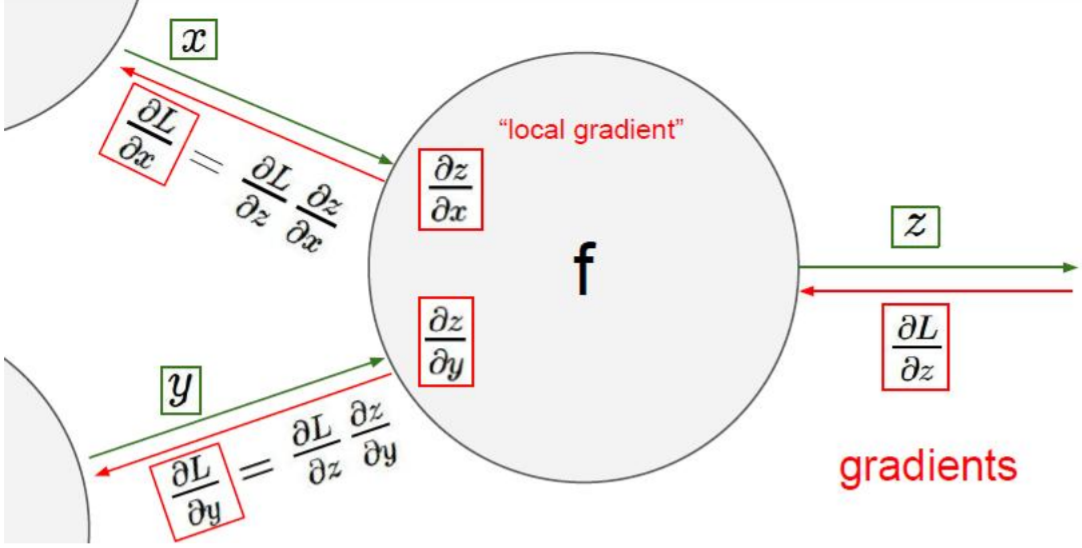
\includegraphics[scale=0.5]{figures/backprop.png}
	\caption{ Прямое распространение сигнала и обратное распространение градиента }\label{fig:backprop}
\end{figure}

\section{Приемы работы с библиотекой \texttt{marshmallow}}

\emph{Сериализация} ({dumping}) -- это процедура преобразования объекта или дерева объектов в какой-либо формат, по которому потом эти объекты можно восстановить. Используется, например, для сохранения состояния программы (то есть некоторых ее объектов) между запусками. Или для передачи данных по сети. 

Основная идея заключается в том, что сериализованный формат -- это \emph{последовательность байт} или \emph{строка}.

Обратная процедура называется \emph{десериализацией} (loading).

Например, для сериализации с помощью модуля \texttt{json} можно поступить так
\begin{lstlisting}[
style = ironpython,
numbers = none
]
import json

d = {"key1": 10, "key2": 20}

# для преобрзвания дерева объектов в последовательность байтов
with open("./make_json.json", mode="w") as f:
    json.dump(d, fp=f) # словарь -> файл

# для преобразования дерева объектов в строку
json.dumps(d)  # вернет строку '{"key1": 10, "key2": 20}'
\end{lstlisting}

Объявим класс данных
\begin{lstlisting}[
style = ironpython,
numbers = none
]
from marshmallow import Schema, fields, validate, ValidationError

# объявляем структуру данных
class PersonSchema(Schema):
    name = fields.String(
        required=True,
        validate=validate.Regexp("^Le.*$")
    )
    age = fields.Integer(
        required=True,
        validate=validate.Range(min=18, max=45)
    )
    job = fields.String(
        required=False,
        validate=validate.Length(min=3)
    )
    email = fields.Email(required=False)
    sex = fields.String(load_default="male")  # это значение по умолчанию будет использоваться на шаге десериализации

# проверка на согласованность 
person_leor = PersonSchema().load({
    "name": "Leor",
    "age": 35,
    "job": "Data Scientist",
    "email": "leor.finkelberg@yandex.ru",
})

type(person_leor)  # dict
\end{lstlisting}

Если переданный словарь отвечает стуктуре данных, то метод \verb*|load()| класса \verb*|PersonSchema| этот же словарь и вернет. Но если хотя бы одно значение нарушает требования поля, то будет возбуждено исключение \verb*|ValidationError|. Поэтому строки вызова метода \verb*|load| следует оборачивать с помощью \verb*|try-except|
\begin{lstlisting}[
style = ironpython,
numbers = none	
]
schema = PersonSchema()
leor = {"name": "Leor", ...}
try:
    # метод load прогоняет словарь через структуру данных
    # и если все хорошо, то этот же словарь и возвращает
    person_leor: dict = PersonSchema().load(leor)
except ValidationError as err:
    print(err.messages, err.valid_data)
\end{lstlisting}


\section{Борьба с переобучением в нейронных сетях}

\subsection{Нормировка}

Пусть даны признаки $ X = \{X_1, \ldots, X_m\} $.

Тогда

\emph{среднее признака}
\begin{align*}
	\mu = \dfrac{1}{m} \sum_{i=1}^m X_i,
\end{align*}

\emph{дисперсия признака}
\begin{align*}
	\sigma^2 = \dfrac{1}{m} \sum_{i=1}^m (X_i - \mu)^2
\end{align*}

\emph{нормировка}
\begin{align*}
	X = \dfrac{X - \mu}{\sqrt{\sigma^2}}
\end{align*}

\subsection{Инициализация весов}

Инициализация весов:
\begin{itemize}
	\item нарушить симметричность (чтобы нейроны были разные),
	
	\item недопустить насыщение нейрона (почти всегда близок к 0 или 1),
	
	\item ключевая идея -- входы на все слои должны иметь одинаковую дисперсию (для избегания <<насыщения>> нейронов).
\end{itemize}

Инициализация по Ксавье [Glorot \& Bengio, 2010]
\begin{align*}
	w_{ij}^{(k)} \sim U \Bigg[ - \sqrt{ \dfrac{ 6 }{ n_{in}^{(k)} + n_{out}^{(k)}} }, + \sqrt{ \dfrac{ 6 }{ n_{in}^{(k)} + n_{out}^{(k)}} } \, \Bigg].
\end{align*}

Дисперсия весов
\begin{align*}
	D[ w_{ij}^{(k)} ] = \dfrac{ 2 }{ n_{in}^{(k)} + n_{out}^{(k)} }.
\end{align*}

Формула выведена в предположении, что нет нелинейностей, т.е. $ z^{(k+1)} = f(W^{(k)} z^{(k)}) \equiv W^{(k)} z^{(k)} $.

Смотрим ошибку на отложенной выборке! Выбираем итерацию, на которой ошибка наименьшая (\pic{fig:lear_rate}).

\begin{figure}[h]
	\centering
	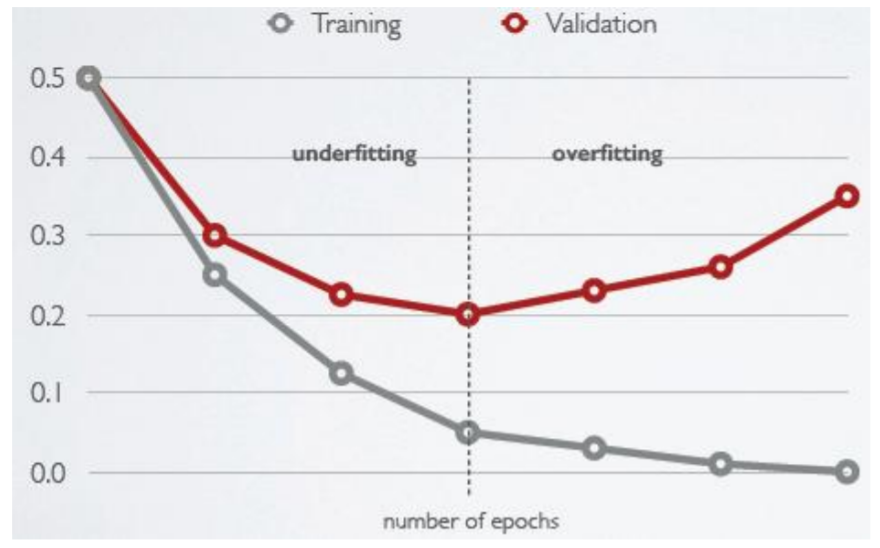
\includegraphics[scale=0.5]{figures/lear_rate.png}
	\caption{ Настройка темпа обучения }\label{fig:lear_rate}
\end{figure}

Увеличение размера пакета -- тот же эффект, что и уменьшение темпа обучения.

\subsection{Продвинутая оптимизация}

Стохастический градиент (надо случайно перемешивать данные перед каждой эпохой)
\begin{align*}
	w^{(t+1)} = w^{(t)} - \eta \, \nabla L^{(t)}(w^{(t)}).
\end{align*}

Стохастический градиент с моментом (Momentum)
\begin{align*}
	m^{(t+1)} = \rho \, m^{(t)} + \nabla L^{(t)}(w^{(t)}),\\
	w^{(t+1)} = w^{(t)} - \eta \, m^{(t+1)} = \underbrace{ w^{(t)} - \eta \, \nabla L^{(t)}(w^{(t)}) }_{\text{\itshape стохастический градиент}}+ \underbrace{- \eta \, \rho \, m^{(t)}}_{\text{\itshape добавление инерции}}.
\end{align*}

Метод Нестерова
\begin{align*}
	m^{(t+1)} = \rho \, m^{(t)} + \nabla L^{(t)} (w^{(t)} - \eta \, m^{(t)}),\\
	w^{(t+1)} = w^{(t)} - \eta \, m^{(t+1)} = w^{(t)} - \eta \, \nabla L^{(t)}(w^{(t)} + \underbrace{\color{blue} - \eta \, m^{(t)}}_{\text{\itshape\color{blue} смещение}}) + \underbrace{\color{blue} - \eta \, \rho \, m^{(t)} }_{\text{\itshape\color{blue} добавление инерции}}.
\end{align*}

\section{Графовые нейронные сети}

Полезные ресурсы Distill
\begin{itemize}
	\item \url{https://distill.pub/2021/understanding-gnns/},
	
	\item \url{https://distill.pub/2021/gnn-intro/}.
\end{itemize}


Графовые нейронные сети (GNN) вычисляют предаставления вершин в итеративном процессе, разные виды GNN по-разному, каждая итерация соответствует слою сети. Самая простая концепция такого вычисления -- неронное распространение (Neural Message Passing). Вообще, распространение сообщений довольно известный прием в анализе графов, заключается в том, что каждая вершина имеет некоторое состояние, которое за одну итерацию уточняется по следующей формуле
\begin{align*}
	h_v^{(k)} = \text{UPDATE}^{(k)} \Big( h_v^{(k-1)},  \text{AGG}^{(k)} (\{ h_u^{(k-1)} \}_{u \in N(v)}) \Big),
\end{align*}
где $ N(v) $ -- окрестной вершины $ v $, $ \text{AGG} $ -- функция аггрегации (по смыслу она собирает информацию о соседях, например, суммируя состояния), $ \text{UPDATE} $ -- функция обновления состояния вершины (с учетом собранной информации о сосдениях).

Единственное требование, которое накладывается на последние две функции -- дифференциируемость, чтобы использовать их в вычислительном графе и вычислять параметры сети методом обратного распространения.

\noindent\emph{Для графовых сверточных нейронных сетей}

\begin{align*}
	h_v^{(0)} = x_v, \ \forall v \in V,
\end{align*}
где $ h_v^{(0)} $ -- начальное представление узла $ v $, $ x_v $ -- оригинальные признаки узла $ v $.

И теперь для каждого шага $ k = 1, 2, \ldots, K $ [Distill]
\begin{align*}
	h_v^{(k)} = f^{(k)} \Big( W^{(k)} \cdot \dfrac{ \sum\limits_{ u \in N(v) } h_u^{(k-1)} }{ |N(v)| } + B^{(k)} \cdot h_v^{(k-1)}\Big), \ \forall v \in V,
\end{align*}
где $ h_v^{(k)} $ -- представление узла $ v $ на шаге $ k $, $ h_v^{(k-1)} $ -- представление узла $ v $ на шаге $ k - 1 $.

\remark{
Веса $ W^{(k)} $ и $ B^{(k)} $ разделяются между всеми узлами графа
}

Выражение справа от коэффициента $ W^{(k)} $ -- среднее представлений соседей вершины $ v $ на шаге $ k - 1 $.

Построить прогноз на каждом узле можно с помощью последнего вычисленного представления
\begin{align*}
	\hat{y}_v = \text{PREDICT}(h_v^{(K)}),
\end{align*}
где $ \text{PREDICT} $ -- как правило, другая нейронная сеть, обученная вместе с моделью GCN.

\remark{
GCN хорошо масштабируется, поскольку количество параметров в модели не привязано к размеру графа
}

Пример (\pic{fig:GCN}). Для вершины $ A $ на шаге 1 представление можно вычислить следующим образом, опросив соседей вершины
\begin{align*}
	h_A^{(1)} &= f\Big( W^{(1)} \times \dfrac{ h_E^{(0)} + h_F^{(0)} + h_G^{(0)} }{ 3 } + B^{(1)} \times h_A^{(0)} \Big) \\
	&= f(1 \times \dfrac{ 2 + (-2) + 0 }{ 3 } + 1 \times -4) \\
	&= f(0 + (-4)) \\
	&= f(-4) \\
	&= ReLU(-4) = 0.
\end{align*}

\begin{figure}[h]
	\centering
	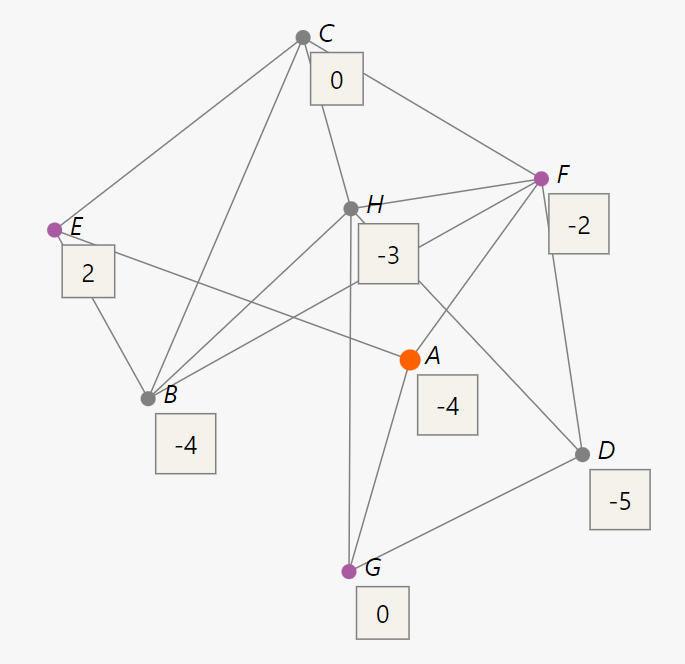
\includegraphics[scale=0.5]{figures/GCN.png}
	\caption{ Пример вычисления обновленного представления узла $ A $ на шаге 1 \\в графовой сверточной нейронной сети }\label{fig:GCN}
\end{figure}

На практике каждая описанная выше итерация обычно рассматривается как один <<слой нейронной сети>>. Этой идеологии придерживаются многие популярные библиотеки графовых нейронных сетей (PyTorch Geometic, StellarGraph), позволяющие создавать различные типы сверток графа в одной и той же модели.

Методы, которые мы рассматривали до сих пор, выполняют <<локальные>> свертки: признак каждого узла обновляется с использованием информации о признаках его локальных соседей. Однако можно построить и <<глобальную>> свертку.

После выбора произвольного порядка узлов мы можем собрать все признаки в вектор $ x \in \mathbb{R} $.

После нормализации $ x $ как $ \sum\limits_{i=1}^n x_i^2 = 1 $
\begin{align*}
	R_L(x) = \dfrac{ x^T Lx }{ x^T x} = \dfrac{ \sum_{(i,j) \in E} (x_i - x_j)^2 }{ \sum_i x_i^2 } = \sum_{ (i, j) \in E } (x_i - x_j)^2.
\end{align*} 

Множество собственных чисел лапласиана $ L $ называют \emph{спектром}. Спектральное разложение
\begin{align*}
	L = U \Lambda U^T, \ \Lambda = \text{diag}(\lambda_1, \ldots, \lambda_n), \ U = \{u_1 \ldots u_n\}, \ U^T U = I,
\end{align*}
где $ \Lambda $ -- диагональная матрица отсортированных собственных чисел, $ U $ -- обозначает матрицу собственных векторов, отсортированных по возрастанию собственных чисел.

Каждый вектор признаков $ x $ может быть представлен в виде линейной комбинации собственных векторов
\begin{align*}
	x = \sum_{i=1}^n \hat{x}_i u_i = U \hat{x},
\end{align*}
где $ \hat{x} $ -- это вектор коэффициентов $ [x_0, \ldots, x_n] $. Будем называть $ \hat{x} $ \emph{спектральным представлением} вектора признаков $ x $.

\remark{
Свертку в спектральной области графа можно рассматривать как обобщение свертки в частотной области изображений
}

Теория спектральных сверток математически обоснована, но есть несколько нюаносов:
\begin{itemize}
	\item Нам требуется вычислить матрицу собственных векторов $ U_m $. Для больших графов это неосуществимо,
	
	\item Даже если мы сможем вычислить $ U_m $, сами глобальные свертки неэффективны из-за повторяющегося умножения,
	
	\item Изученные фильтры специфичны для графов, поскольку они представлены в терминах спектрального разложения входного графа Лапласиана. Это означает, что они плохо переносятся на новые графы, которые имеют существенно иную структуру (и, следовательно, существенно разные собственные значения).
\end{itemize}

Хотя спекртальные свертки в значительной степени были вытеснены <<локальными>> свертками по рассмотренным выше причинам, все еще имеет смысл изучать идеи, лежащие в их основе.

Функции потерь для различных задач на графах:
\begin{itemize}
	\item Классификация узлов:
\begin{align*}
	\mathcal{L}(y_v, \hat{y}_v) = - \sum_c y_{vc} \log \hat{y}_{vc},
\end{align*}
где $ \hat{y}_{vc} $ -- предсказанная вероятность того что узел $ v $ принадлежит классу $ c $. GNNs адаптированы и для обучения на частично-размеченных данных, когда только некоторые узлы имеют разметку. В этом случае функцию потерь можно так
\begin{align*}
	\mathcal{L}_G = \dfrac{ \sum\limits_{ v \in \text{ Lab }(G) } \mathcal{L}(y_v, \hat{y}_v)}{ | \text{Lab}(G) | },
\end{align*}
где потери можно вычислить только на размеченных узлах $ \text{Lab}(G) $.

    \item Классификация графа: собрав информацию о представлении узлов графа, можно составить векторное представление графа. 
    
    \item Предсказание вероятности появления связи: опираясь на пары смежных и несмежных узлов, можно использовать их векторные представления в качестве входных данных для прогнозирования наличия / отсутствия связи
\begin{align*}
	\mathcal{L}(y_v, y_u, e_{vu}) = - e_{vu} \log (p_{vu}) - (1 - e_{vu}) \log(1 - p_{vu}),\\
	p_{vu} = \sigma (y_v^T y_u),
\end{align*}
где $ \sigma $ -- логистический сигмоид, и $ e_{vu} = 1 $, если между узлами $ v $ и $ u $ есть связь, и $ e_{vu} = 0 $ в противном случае.

    \item Кластеризация узлов: простая кластеризация представлений узлов.
\end{itemize}

Основная проблема при использовании описываемого нейронного распространения, т.н. \emph{чрезмерное сглаживание} (over-smoothing): после нескольких итераций пересчета состояний вершин представления соседних вершин становятся похожими, поскольку у них похожие окрестности. Для борьбы с этим делают
\begin{itemize}
	\item меньше слоев агрегации и больше для <<обработки признаков>>,
	
	\item прокидывание слоев или конкатенацию состояний с предыдущих слоев,
	
	\item используют архитектуры, в которых есть эффект памяти,
	
	\item приемы с номировками,
	
	\item используют аугментацию, например, DropEdge,
	
	\item используют noise regularization.
\end{itemize}

Сводка по графовым нейронным сетям
\begin{itemize}
	\item На вход сети подается граф, каждая вершина которого имеет признаковое описание. Это описание можно считать начальным состоянием вершины,
	
	\item Могут быть слои, которые независимо модифицируют представления (для каждой вершины его представление пропускается через небольшую нейронку),
	
	\item Могут быть слои, которые модифицируют представления всех вершин, учитывая представления вершин-соседей,
	
	\item Могут быть слои, упрощающие граф (например, уменьшающие число вершин),
	
	\item Могут быть слои, получающие представление графа (вектор фиксированной длины) по текущему графу с представлениями вершин.
\end{itemize}



\section{Отбор признаков с библиотекой BoostARoota}

BoostARoota \url{https://github.com/chasedehan/BoostARoota} -- алгоритм отобора признаков на базе экстримального градиентного бустинга в реализации XGBoost. Алгоритм требует гораздо меньших затрат времени на выполнение. Перед применением необходимо выполнить дамми-кодирование, поскольку базовая модель работает только с количественными признаками.

Отбор признаков выполняется на обучающем поднаборе данных, поэтому предполагается, что массив меток и массив признаков \emph{обучающие}, а для проверки качества модели отбора признаков есть независимая, \emph{тестовая} выборка. Кроме того, если необходимо выбрать оптимальные значения гиперпараметров модели отбора признаков (например, значения гиперпараметров \texttt{cutoff}, \texttt{iters} и \texttt{delta}), то понадобиться еще \emph{проверочная} {выборка}.

\section{Классический и байесовский бутстреп}

Бутстреп является универсальным инструментом для оценки статистической точности. 

Байесовский бутстреп это байевоский аналог классического бутстрапа. Вместо моделирования распределения выборки для статистики, оценивающей параметр, байесовский бутстреп моделирует \emph{апостериорное распределение параметра}. 

Основная идея состоит в том, чтобы случайным образом извлекать наборы данных с \underline{возвращением} из обучающих данных так, чтобы каждая выборка имела тот же размер, что и исходное обучающее множество.Это делается $ B $ раз (скажем, $ B = 100 $), создавая $ B $ множеств бутстрепа. Затем мы заново аппроксимируем модель для каждого из множест бутстрепа и исследуем поведение аппроксимаций на $ B $ выборках.

По выборке бутстрепа мы можем оценить любой аспект распределения $ S(\mathbf{Z}) $ (это любая величина, вычисленная по данным $ \mathbf{Z} $), например, его дисперсию
\begin{align*}
	\widehat{ Var }[ S(\mathbf{Z}) ] = \dfrac{1}{B - 1} \sum_{b=1}^{B} \Big( S(\mathbf{Z}^{*b})  - \bar{S}^* \Big)^2, \quad \bar{S}^{*} = \sum_b S( \mathbf{Z}^{*b} ) / B.
\end{align*}

\section{HDI}

Highest Density Interval (HDI) -- интервал высокой плотности -- показывает какие точки распределения наиболее достоверны/правдоподобны и охватывают большую часть распределения. Каждая точка внутри интервала имеет более высокую \emph{достоверность}, чем любая точка вне интервала.

\section{Площадь по ROC-кривой}

Построение ROC-кривой происходит следующим образом (\pic{fig:roc_auc0}):
\begin{enumerate}
	\item  Сначала сортируем все наблюдения по убыванию спрогнозированной вероятности положительного класса,
	
	\item Берем единичный квадрат на координатной плоскости. Значения оси абсцисс будут значениями 1 - специфичности (цена деления оси задается значением 1/neg), а значения оси ординат будут значениями чувствительности (цена деления оси задается значением 1/pos). При этом pos — это количество наблюдений положительного класса, а neg — количество наблюдений отрицательного класса,
	
	\item Задаем точку c координатами (0, 0) и для каждого отсортированного наблюдения x:
	\begin{itemize}
		\item если x принадлежит положительному классу, двигаемся на 1/pos вверх,
		
		\item если x принадлежит отрицательному классу, двигаемся на 1/neg вправо.
	\end{itemize}
\end{enumerate}

Значение вероятности положительного класса, при котором ROC-кривая находится на минимальном расстоянии от верхнего левого угла -- точки с координатами (0, 1), дает наибольшую правильность классификации. В данному случае (\pic{fig:roc_auc0-1}) будет 0.72.

\begin{figure}[h]
	\centering
	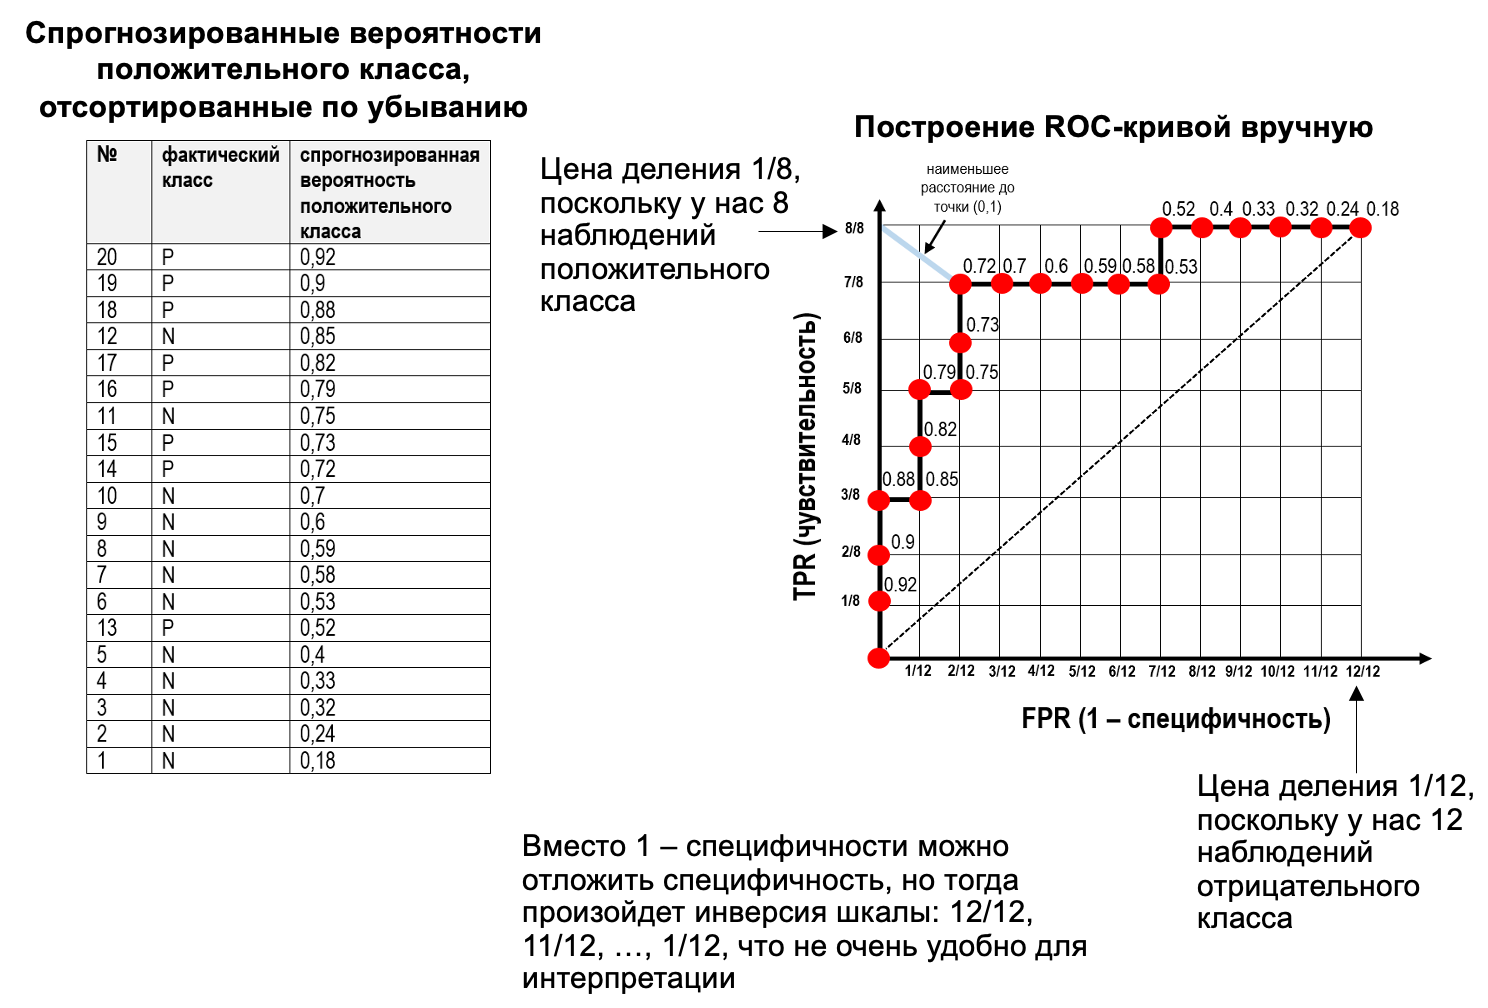
\includegraphics[scale=0.3]{figures/roc_auc0.png}
	\caption{ Построение ROC-кривой }\label{fig:roc_auc0}
\end{figure}

\begin{figure}[h]
	\centering
	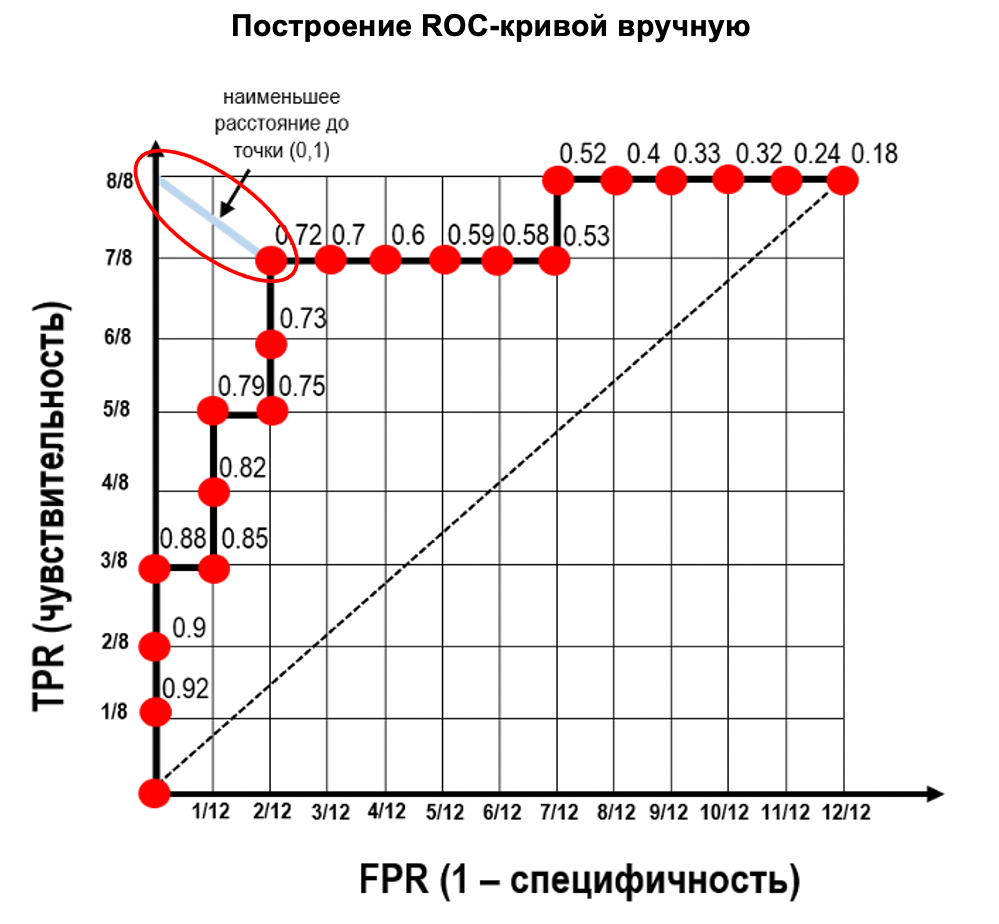
\includegraphics[scale=0.3]{figures/roc_auc0-1.png}
	\caption{ ROC-кривая. Порог отсечения 0.72 }\label{fig:roc_auc0-1}
\end{figure}

Площадь под ROC-кривой (ROC-AUC) можно интерпретировать как вероятность события, состоящего в том, что классификатор присвоит более высокий ранг (например, вероятность) случайно выбранному экземпляру положительного класса, чем случайно выбранному экземпляру отрицательного класса (если не рассматривать вариант равенства значений рангов).

\remark{
На ROC-кривые не влияет баланс классов (при достаточном объеме выборки) и они могут чрезмерно оптимистично оценивать качество работы алгоритма в случае дисбалансов. Лучше пользоваться гармоническим средним или PR-кривыми
}

Однако недостаток такой интепретации заключается в том, что мы пренебрегаем часто встречающейся ситуацией равенства вероятностей. Поэтому правильнее будет сказать, что ROC-AUC равен доле пар вида (экземпляр положительного класса, экземпляр отрицательного класса), которые алгоритм верно упорядочил в соответствии с формулой
\begin{align}\label{eq:rocauc}
	\dfrac{ \sum\limits_{i, j=1}^{n_i, n_j} s(x_i, x_j)}{ n_i \, n_j }, \quad s(x_i, x_j) =
	\begin{cases}
		1, x_i > x_j,\\
		1/2, x_i = x_j,\\
		0, x_i < x_j,
	\end{cases}
\end{align}
где $ x_i $ -- ответ алгоритма для положительного экземпляра, $ x_j $ -- ответ алгоритма для отрицательного экземпляра.

По сути числитель дроби представляет собой сумму количеств $ j $-ых наблюдений отрицательного класса, лежащих ниже каждого $ i $-ого наблюдения положительного класса. Каждое такое количество мы берем по каждому $ i $-ому наблюдению положительного класса в последовательности, отсортированной по мере убывания вероятности положительного класса. Знаменатель дроби -- это произведение количества наблюдений положительного класса и наблюдений отрицательного класса.

Если говорить более точно, мы берем наблюдение положительного класса под номером 20 и каждый раз образовываем пару с наблюдением отрицательного класса (\pic{fig:roc_auc1}), у нас 12 пар, 12 раз наблюдение полжительного класса под номером 20 было проранжировано выше наблюдений отрицательного класса 12, 11, 10 и т.д. Записываем число 12 напротив наблюдения 20. 

Разные модели нельзя сравнивать только по ROC-AUC. ROC-AUC оценивает разные классификатор, используя метрику, которая сама зависит от классификатора. То есть ROC-AUC оценивает разные классификаторы, используя разные метрики.

\remark{
Если часть ROC-кривой лежит ниже диагональной линии, а часть -- выше, то это означает, что классы не являются линейно-сепарабельными, а при этом используется линейная модель
}

При одинаковой ROC-AUC у разных моделей (соответственно с разными ROC-кривыми) будет разное распределение стоимостей ошибочной классификации. Проще говоря, мы можем вычислить ROC-AUC для классификатора A и получить 0.7, а затем вычислить ROC-AUC для второго классификатора и снова получить 0.7, но это не обязательно означает, что у них одна и та же эффективность.

\emph{Задача} Чему равно значение метрики ROC AUC у классификатора, который для любого объекта возвращает значение 0.97, если доля положительного класса в выборке составляет 4\%?

Первый способ. Вероятностная интерпретация. Метрика ROC AUC показывает долю верно упорядоченных пар. Константный классификатор не задает никакого порядка объектов. Это значит, что они упорядочиваются \emph{случайным образом}. А ROC AUC случайного классификатора равен 0.5.

Второй способ. При отрисовке ROC-кривой, в случае одинаковых ответов классификатора, необходимо двигаться и вверх, и вправо одновременно. Значение всего одно, значит прямая тоже одна -- это просто диагональная линия. Площадь получившегося треугольника 0.5.



\section{Приемы работы с Gurobi}

Полезный ресурс \url{https://www.gams.com/latest/docs/S_GUROBI.html#GUROBI_GAMS_GUROBI_LOG_FILE}

Чтобы запустить Gurobi в интерактвином режиме, следует в командной оболочке набрать \texttt{gurobi}
\begin{lstlisting}[
title = {\sffamily Сессия GUROBI},
style = bash,
numbers = none
]
gurobi> m = read("./ikp_milp_problem.lp")
gurobi> m.optimize()
gurobi> vars = m.getVars()
gurobi> help(m)
# вывести 2-картежи целочисленных переменных с отличным от нуля значением
gurobi> [(var.varName, var.x) for var in vars if (var.x > 0) and (var.vType == "I")]
gurobi> m.write("res.sol")  # записать решение
gurobi> help(GRM.param)  # параметры GUROBI
gurobi> m.getParamInfo("TimeLimit")  # ('TimeLimit', <class 'float'>, inf, 0.0, inf, inf)
gurobi> m.getParamInfo("MIPGap")  # ('MIPGap', <class 'float'>, 0.0001, 0.0, inf, 0.0001)
gurobi> m.setParam("MIPGap", 65)
gurobi> m.setParam("TimeLimit", 100)
\end{lstlisting}


\begin{figure}[h]
	\centering
	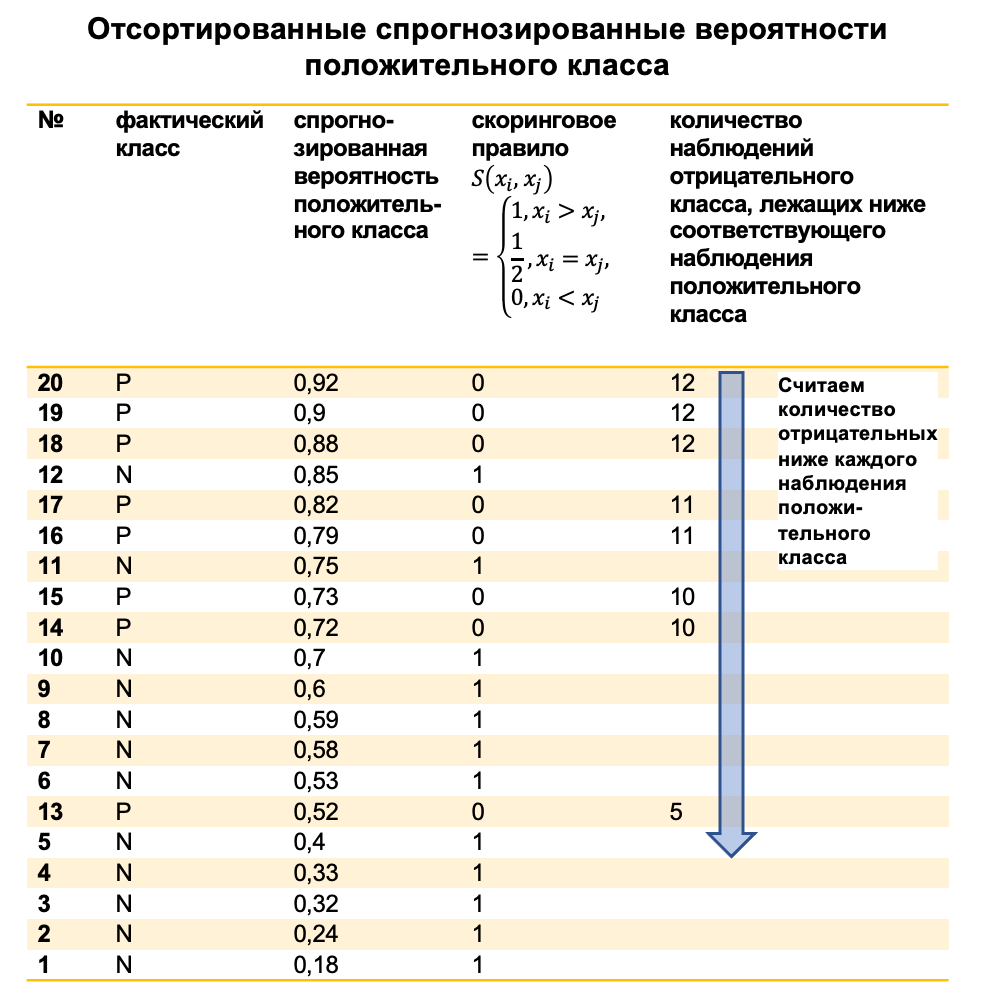
\includegraphics[scale=0.35]{figures/roc_auc1.png}
	\caption{ Расчет ROC-AUC по формуле \eqref{eq:rocauc}}\label{fig:roc_auc1}
\end{figure}

\begin{figure}[h]
	\centering
	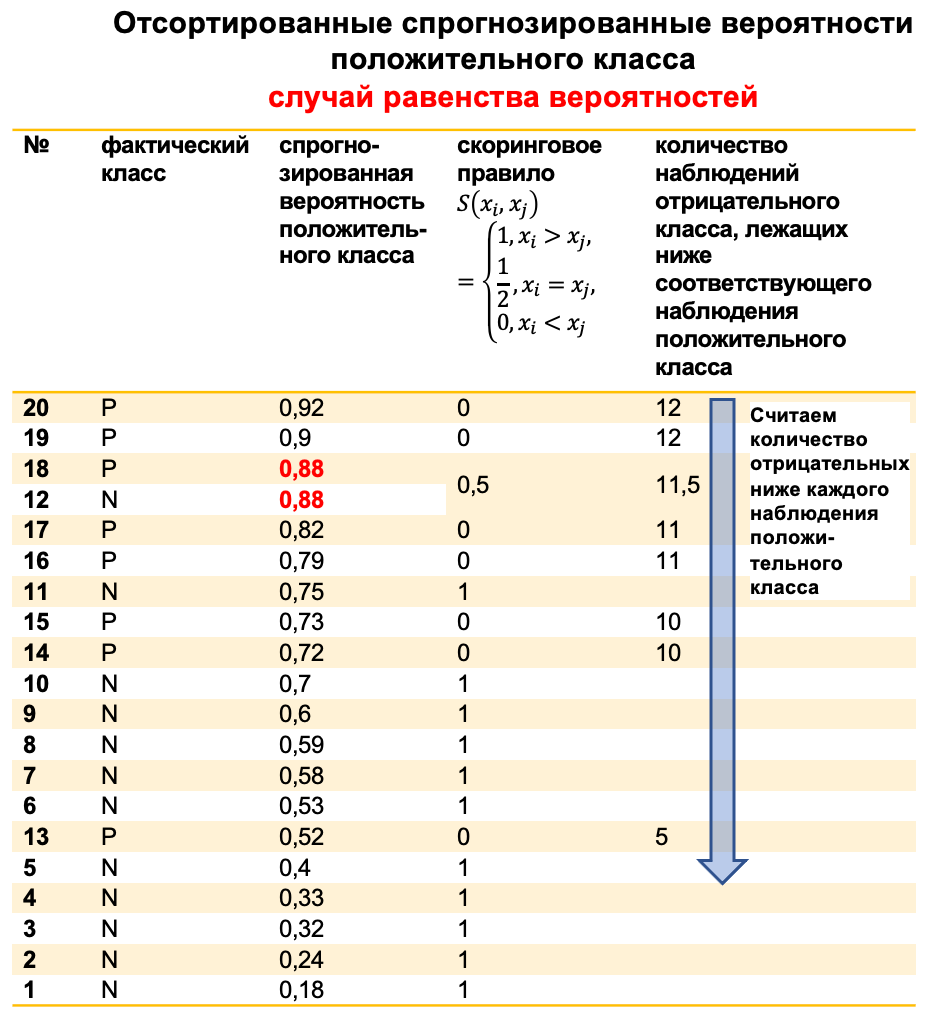
\includegraphics[scale=0.35]{figures/roc_auc2.png}
	\caption{ Расчет ROC-AUC по формуле \eqref{eq:rocauc} для случая равных вероятностей принадлежности экземпляра положительному классу}\label{fig:roc_auc2}
\end{figure}

\section{Кластеризация. K-means, MeanShift, Affinity Prop, HDBSCAN и детектор выборосов GLOSH}

\subsection{Краткая сводка по основным кластеризаторам}

\url{https://hdbscan.readthedocs.io/en/latest/comparing_clustering_algorithms.html#k-means}

\subsubsection{KMeans}

K-means быстрый, простой, легко интерпретируется. Однако, у него есть несколько проблем. Во-первых, строго говоря, это не алгоритм кластеризации, а алгоритм партицианирования. То есть K-Means <<не ищет>> кластеры, а просто разбивает набор данных на заданное число <<сферических>> партиций (фрагментов). Отсюда вторая проблема. Нужно указать ожидаемое число кластеров.

K-Means зависит от инициализации. Различные случайные запуски будут приводить к различным результатам кластеризации. K-Means предполагает, что кластеры гиперсферические, и не умеет детектировать шумовые точки.

K-Means вычислительно эффективен и на по-настоящему больших данных может остатся единственным вариантом.

\subsubsection{Affinity Propagation}

Как и K-Means предполагает, что кластеры гиперсферические и не умеет детектировать шумовые точки. Не нужно задавать число кластеров, но <<правильные>> значения его параметров \texttt{preference} и \texttt{damping} на практике найти не просто.

Очень медленный алгоритм.

\subsubsection{MeanShift}

Умеет выявлять шумовые точки, но так же как и K-Means предполагает кластеры гиперсферическими. Имеет параметры с более прозрачным смыслом. Зависит от инициализации (производительность может гулять).

Все-таки медленный алгоритм.

\subsubsection{Spectral Clustering}

Не предполагает, что кластеры гиперсферические, но не умеет выявлять шумовые точки (то есть кластеры загрязняются шумом). Нужно задавать число кластеров.

Медленный алгоритм.

\subsubsection{Agglomerative Clustering}

Не выдвигает гипотезы о гиперсферичности кластеров, но не умеет выявлять шумовые точки. Нужно задавать число кластеров.

sklearn-реализация очень медленная.

\subsubsection{DBSCAN}

Кластеры не обязательно должны быть сферическими. Умеет детектировать шумовые точки. Скопления переменной плотности могут стать проблемой. Параметр $ \varepsilon $ на практике настроить нелегко. Обычно у алгоритма высокая производительность, но на наборах порядка 1'000'000 экзмепляров все-таки работает не очень быстро.

Классический DBSCAN в отличие от DBSCAN* кроме \emph{ядровых} (core objects) и \emph{шумовых} (noise objects) экземпляров используется еще и \emph{граничные} экземпляры (border objects).

\subsubsection{HDBSCAN}

Может эффективно работать на класетрах переменной плотности. Не делает предположения о гиперсферичности кластеров. Умеет выявлять шумовые точки. Не требует задавать параметр $ \varepsilon $. Вместо него используется параметр \texttt{min\_cluster\_size}. Очень эффективная реализация.

\subsection{Одноклассовая классификация}

В отличие от классической задачи классификация, в одно-классовой классификации нам предоставляются только наблюдения одного класса, а модель должна сообщить принадлижат ли новые наблюдения этому классу или нет.

Если в задаче бинарной классификации требуется, чтобы модель разбила пространство признаков на две области, представляющие свой класс, то в одно-классовой классификации модель должна определить подобласть в пространстве признаков, точки которой будут считаться <<нормальными>>, а точке вне этой подобласти -- выбросами (\pic{fig:binary_and_oneclass}).

\begin{figure}[!h]
	\centering
	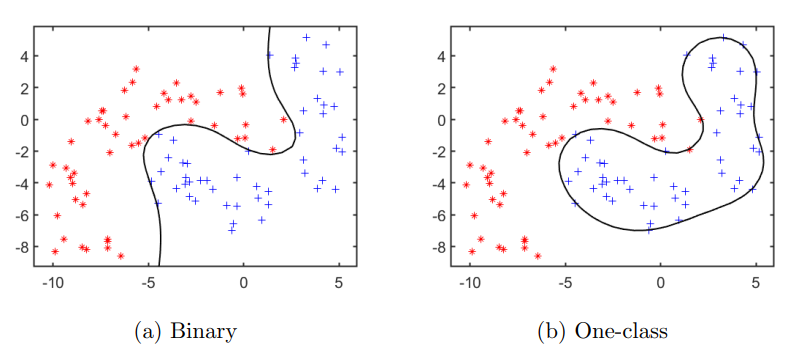
\includegraphics[scale=1.]{figures/binary_and_oneclass_classifiers.png}
	\caption{ Бинарная и одно-классовая классификация }\label{fig:binary_and_oneclass}
\end{figure}

\subsection{Обнаружение выборосов с помощью GLOSH}

GLOSH (Global-Local Outlier Score from Hierarchies) -- это алгоритм обнаружения выборосов без использования информации о разметке, основанный на иерархический оценках плотности, предоставляемых HDBSCAN*.

Оценка по GLOSH (грубо можно интерпретировать как уверенность в том, что рассматриваемый экземпляр является выбросом) определяется следущим образом
\begin{align*}
	\text{GLOSH}(x_i) = \dfrac{ \lambda_{\max} (C_{x_i}) - \lambda(x_i) }{ \lambda_{\max}(C_{x_i}) },
\end{align*} 
где $ \lambda(x_i) $ -- плотность экземпляра $ x_i $; $ \lambda_{\max}(C_{x_i}) $ -- плотность экземпляра $ x_l \in C_{x_i} $ с набольшей плотностью, где плотности определяются по порогу плотности $ \varepsilon $ -- уровню плотности, отвечающему экземпляру помеченному как <<шумовой>> в иерархии HDBSCAN*.

Оценки по GLOSH принимают значения из диапазона $ [0, 1) $, где оценка 0 означает, что экземпляр считается <<штатным>>, а оценки близкие к 1 указывают на то, что есть основания считать экземпляр выбросом\footnote{The higher the score, the more likely the point is to be an outlier \url{https://hdbscan.readthedocs.io/en/latest/outlier_detection.html}}.




\listoffigures\addcontentsline{toc}{section}{Список иллюстраций}

% Источники в "Газовой промышленности" нумеруются по мере упоминания 
\begin{thebibliography}{99}\addcontentsline{toc}{section}{Список литературы}
	\bibitem{lutz:learningpython-2011}{\emph{Лутц М.} Изучаем Python, 4-е издание. -- Пер. с англ. -- СПб.: Символ-Плюс, 2011. -- 1280~с. }
	
	\bibitem{geron:hands_on_ml}{\emph{Жерон О.} Прикладное машинное обучение с помощью Scikit-Learn и TensorFlow: концепции, инструменты и техники ля создания интеллектуальных систем. -- СПб.: ООО <<Альфа-книга>>, 2018. -- 688 с.}
	
	\bibitem{burkov:2020}{\emph{Бурков А.} Машинное обучение без лишних слов. -- СПб.: Питер, 2020. -- 192 с.}
	
	\bibitem{burkov-engineer:2022}{\emph{Бурков А.} Инженерия машинного обучения. -- М.:ДМК Пресс, 2022. -- 306 с.}
	
	\bibitem{lakshmanan-mldp:2022}{\emph{Лакшманан В.} Машинное обучение. Паттерны проектирования. -- СПб.: БХВ-Перетбург, 2022. -- 448 с.}
		
	\bibitem{beazley:python-2010}{\emph{Бизли Д.} Python. Подробный справочник. -- Пер. с англ. -- СПб.: Символ-Плюс, 2010. -- 864~с. }
	
	\bibitem{dart:2015}{\emph{Rashmi K.V.}, \emph{Gilad-Bachrach R.} DART: Dropouts meet Multiple Additive Regression Trees, 2015}
	
	\bibitem{ke-lightgbm:2017}{\emph{Ke G. etc.} LightGBM: A Highly Efficient Gradient Boosting Decision Tree, 2017}
\end{thebibliography}

\end{document}
